\documentclass[a4paper]{book}
\usepackage[czech]{babel}
\usepackage[utf8]{inputenc}
\usepackage{pstricks}
\usepackage{amsmath}
\usepackage{graphicx}
\usepackage{multirow}

\setlength{\unitlength}{1.0mm}

\begin{document}

\title{Finanční instrumenty s fixním cash-flow}
\author{L.Martellini, P.Priaulet, S.Priaulet}
\date{2003}
\maketitle

\tableofcontents

\part{Investiční prostředí}

\chapter{Dluhopisy a instrumenty peněžního trhu}

Tato kapitola je přehledem základních instrumentů s fixním cash-flow, konkrétně pak dluhopisů a instrumentů peněžního trhu.

\section{Dluhopisy}

\subsection{Obecná charakteristika dluhopisů}

\subsubsection{Definice standardního dluhopisu}

Dluhopis je cenný papír, který zavazuje svého emitenta k úhradě nominální hodnoty dluhopisu jeho majiteli v době splatnosti a popř. také k periodické výplatě úroků. Dluhopis tak z pohledu emitenta představuje alternativu k úvěru má tedy charakter tzv. dluhového cenného papíru.

Naproti tomu akcie je tzv. majetkovým cenným papírem. Její majitel má právo podílet se na zisku společnosti, nemá však právo na splacení nominální hodnoty akcie. Dluhopis je tak v porovnání s akcií méně rizikovou investicí. Dále je s vlastnictvím akcie, narozdíl od dluhopisu, zpravidla spojeno právo podílet se řízení společnosti.

\subsubsection{Terminologie a konvence}

Každý dluhopis je charakterizován tzv. emisními podmínkami, které obsahují veškeré s ním související údaje. Jedná se zejména o
\begin{itemize}
\item jméno emitenta
\item typ emitenta - v případě korporátních dluhopisů se zpravidla jedná o specifikaci odvětví
\item trh, na kterém je dluhopis emitován
\item domicil emitenta
\item měnu, ve které je dluhopis emitován
\item metodu, podle které jsou vypočteny cena a výnos dluhopisu
\item typ případných záruk - např. vládní záruky, splátky podkladových hypotečních úvěrů
\item datum splatnosti
\item typ kupóny - fixní, floatový kupón
\item výše kupónu
\item frekvence vyplácení kupónu
\item konvence pro stanovení počtu dní - Actual/Actual, Actual/365, Actual/360 a 30/360
\item den, ke kterému je emise oznámena a nabídnuta potenciálním investorům
\item den, od kterého začíná nabíhat úrok
\item vypořádací den - den, ke kterému proběhne fyzická platba výměnou za dluhopis; obecně se jedná o den uzavření obchodu navýšený stanovený počet pracovních dní (např. ve Spojených státech se pro státní dluhopisy používá konvence den uzavření obchodu plus jeden pracovní den, v Euro zóně se pak tato konvence liší podle konkrétního státu)
\item datum první výplaty kupónu
\item emisní cena
\item spread v době emise - jedná se o spread imlikovaný emisní cenou, kde srovnávací základnou je zvolený státní dluhopis
\item identifikační kód dluhopisu - zpravidla ISIN (International Securities Identification Number) nebo CUIPS (Committee on Uniform Securities Indentification Procedures)
\item rating dluhopisu přiřazený některou z ratingových agentur
\item celkový objem emise
\item část celkové emise, která dosud nebyla upsána investory
\item minimální část objemu emise, kterou lze koupit
\item nominální hodnota dluhopisu
\item cena zpětného odkupu v době splatnosti - zpravidla 100\% nominální hodnoty dluhopisu
\end{itemize}

\begin{figure}
  \includegraphics[bb=0 0 350 250]{czgb.bmp}
  \caption{Charekteristika českého státního dluhopisu (zdroj: Bloomberg)}
  \label{czgb}
\end{figure}

\subsubsection{Tržní kotace}

Hodnota dluhopisu je zpravidla kotována ve formě ceny, výnosové míry do splatnosti nebo spreadu oproti vybranému dluhopisu.\\

Cena dluhopisu kotovaná trhem je zpravidla tzv. netto cena (clean price), která je definovaná jako tzv. brutto cena (gross price) snížená o naběhlý úrok (accrued interest). Brutto cena je definována jako současná hodnota všech budoucích kupónů. Cena, ať už netto nebo brutto, je vyjádřena jako procento z nominální hodnoty dluhopisu. Naběhlý úrok, tj. rozdíl mezi brutto a netto cenou, je roven aktuálně naběhlé části kupónové platby a koresponduje tak s dobou, po kterou kterou dluhopis držel jeho původní majitel\footnote{Brutto a netto cena jsou tedy shodné v den výplaty kupónu.}.

Výnosová míra do splatnosti (yield to maturity, zkráceně též YTM) představuje diskontní sazbu, pro kterou se rovná diskontované cash-flow generované dluhopisem jeho brutto ceně. Výnosová míra do splatnosti je v praxi nejběžnějším způsobem kotace ceny dluhopisu.

Korporátní dluhopisy jsou zpravidla kotovány formou rozdílu jejich výnosové míry do splatnosti a výnosové míry do splatnosti vybraného státního dluhopisu, který slouží jako srovnávací základna. Rozdíl ve výnosových mírách nazýváme spreadem.\\

U každého obchodovaného dluhopisu jsou zpravidla uváděny tzv. bid a ask kotace. V případě, že je hodnota dluhopisu vyjádřena pomocí ceny, představuje bid kotace cenu, za kterou je kotátor ochoten dluhopis koupit a ask kotace cenu, za kterou je ochoten dluhopis prodat. Je zřejmé, že cena bid je nižší než cena ask. V případě výnosové míry do splatnosti popř. spreadu je bid kotace vyšší než ask kotace\footnote{Vyšší výnosová míra resp. spread implikuje nižší cenu dluhopisu a naopak.}. Rozdíl mezi kotací bid a ask je označován jako bid-ask spread a jedná se o jednu z forem transakčních nákladů. Bid-ask spread je také ukazatelem likviditidy daného dluhopisu. V případě korporátních dluhopisů s nižším ratingem denominovaných v méně obvyklé měně může představovat až deset procentních bodů v ceně. Naproti tomu v případě státních cenných papírů emitovaných vládou Spojených států se zpravidla jedná o rozdíl do jedné desetiny procentního bodu v ceně. Vedle pojmu bid a ask kotace se lze setkat také s pojmem kotace mid - jedná se o prostý průměr bid a ask kotace. 

\subsection{Typologie dluhopisů}

\subsubsection{Rozdělení dluhopisů s ohledem na stanovení kupónových plateb}

Fixní dluhopisy (fixed bond) jsou kupónové dluhopisy, které mají po celou dobu své splatnosti konstatní kupónovou sazbu. Cash-flow generované fixním dluhopisem je tak dáno sérií kupónů a nominální hodnotou na konci životnosti.

Floatové dluhopisy (floating rate bond) mají na rozdíl od fixních dluhopisů proměnlivou kupónovou sazbou. Ta je odvozena v předem dohodnutý den podle referenční veličiny\footnote{Jako referenční veličina je zpravidla zvolena úroková sazba - např. šestiměsíční sazba PRIBOR.}. Cash-flow se tak skládá z kupónu odpovídajícího aktuálně zafixované kupónové sazbě, následných kupónů odhadovaných pomocí tzv. forwardových sazeb a nominální hodnoty v době splatnosti dluhopisu.

Diskotní dluhopisy (zero-cupoun bond) negenerují kupónové platby. Výnos je představován rozdílem mezi nákupní cenou dluhopisu a jeho nominální hodnotou.

Stripové dluhopisy (strip bond - Separate Trading of Registered Interest and Principal) jsou diskontní dluhopisy, které vznikly rozdělením státních dluhopisů na jednotlivé kupónové platby a nominál. Podkladovým dluhopisem je téměř výhradně státní dluhopis. Tento typ instrumentu je poměrně oblíbený u subjektů jako jsou např. penzijní fondu, protože umožňuje zafixování výnosové míry v dlouhodobém investičním horizontu. V případě kupónových dluhopisů musí investor řešit problém s investováním vyplácených kupónů. Tím podstupuje tzv. reinvestiční riziko, které se realizuje, pokud je výnosová míra z reinvestovaných kupónů nižší než výnosová míra dluhopisu. Ačkoliv jsou stripové dluhopisy relativně likvidní, jsou méně likvidní než odpovídající státní dluhopisy. To má za následek také větší bid-ask spread.

Inflačně indexované dluhopisy (inflation-index bond) představují speciální typ floatových dluhopisů, jejichž kopónové platby jsou vázány na vývoj inflace. Hlavní motivací pro držení těchto dluhopisů je zajištění se před růstem cenové hladiny. Inflačně indexované dluhopisy jsou emitovány zejména vládami s cílem deklarovat zájem na udržení nízké míry inflace. Nejrozšířenější je tento druh dluhopisu ve Spojeném království a Spojených státech.

\subsubsection{Rozdělení dluhopisů podle emitenta}

Státní dluhopisy (government bond) jsou dluhopisy emitované vládou. Tyto dluhopisy jsou zpravidla denominované v měně příslušné země, ale není to vždy pravidlem (např. dluhopisy emitované polskou vládou denominované v USD). Dluhopisy, které jsou obchodovány častěji než ostatní a mají specifickou zbytkovou splatnost\footnote{Zpravidla se jedná o zbytkovou splatnost dva, pět a deset let.}, slouží jako indikátory trhu a označujeme je jako referenční dluhopisy.

Dluhopisy mohou být emitovány také některou ze státem zřízených institucí, které plní veřejný zájem (např. podpora exportu, poskytovaní hypotečních úvěrů). Tyto dluhopisy zpravidla obsahují určitou formu státní garance a je možné na ně pohlížet jako na quasi státní dluhopisy.

Municipální dluhopisy (municipal bond) jsou dluhopisy emitovány městy, kraji, federálními státy popř. dalšími územně správními celky. Tyto dluhopisy slouží k financování jejich investičních záměrů a mohou s nimi být spojeny daňové úlevy a popř. vládní záruky.

Korporátní dluhopisy (corporate bond) jsou emitovány subjekty soukromého sektoru. Tyto dluhopisy jsou v porovnání se státním dluhopisy charakteristické nižší likviditou a vyšším bid-ask spreadem.\\

S rozdělením dluhopisů dle emitenta je také úzce spojeno tzv. kreditní riziko. Toto riziko představuje pravděpodobnost, s jakou emitent nedodrží své závazky. V případě realizace kreditního rizika\footnote{Závazky emitenta jsou definovány v emisních podmínkách dluhopisu. Realizací kreditního rizika se zpravidla rozumí nesplácení kupónových plateb popř. nominální hodnoty dluhopisu a vyhlášení úpadku emitenta, avšak může mít také např. podobu snížení ratingu emitenta.} hovoříme o defaultní události. Nejnižší kreditní riziko mají obecně státní a nejvyšší korporátní dluhopisy. Kreditní riziko dluhopisu je možné vyjádřit pomocí ratingu nebo pomocí spreadu vztaženého k vhodně zvolené srovnávací základně (standardně ke státnímu dluhopisu s podobnou splatností popř. ke swapové křivce).

\section{Instrumenty peněžního trhu}

Dluhopisy mají v době emise splatnost vyšší než jeden rok. Naproti tomu instrumenty peněžního trhu mají v době emise splatnost zpravidla do jednoho roku a představují tak krátkodobý finanční instrument.

\subsection{Typologie instrumentů peněžního trhu}

\subsubsection{Podkladniční poukázky}

Pokladniční poukázka (T-bill, treasury bill) je státním cenným papírem, který má v době své emise splatnost do jednoho roku. Pokladniční poukázka má podobu diskontního dluhového instrumentu - negeneruje tedy žádné kupónové platby. Ceny jsou zpravidla kotovány je formě výnosu na diskotní bázi popř. na bázi peněžního trhu a to v závislosti na zemi emitenta.

Výnos na diskotní bázi lze vypočíst jako
\begin{equation*}
y_d = \frac{F - P}{F}\frac{B}{n}
\end{equation*}
kde $F$ představuje nominální hodnotu, $P$ cenu podkladniční poukázky, $B$ počet dní v roce (360 popř. 365) a $n$ je počet kalendářních dní do splatnosti. Jestliže známe výnosovou míru, lze cenu podkladniční poukázky vypočíst podle
\begin{equation*}
P = F\Bigg(1 - y_d\frac{n}{B}\Bigg)
\end{equation*}
Výnos na bázi peněžního trhu je roven
\begin{equation*}
y_m = \Bigg( \frac{F}{B} - 1 \Bigg) \frac{B}{n}
\end{equation*}
Vztah mezi výnosem na diskotní bázi a výnosem na bázi peněžního trhu je dán rovnicí
\begin{equation*}
y_m = \frac{B \cdot y_d}{B-n \cdot y_n}
\end{equation*}
Známe-li výnos na bázi peněžního trhu, lze cenu pokladniční poukázky vypočíst jako
\begin{equation*}
P = \frac{F}{\Bigg( 1 + y_n\frac{n}{B}\Bigg)}
\end{equation*}

\subsubsection{Depositní certifikáty}

Depozitní certifikát je dluhový instrument emitovaný bankami s cílem financovat své úvěrové aktivity. Splatnost depozitního certifikátu může být od několika málo týdnů až po několik let. Existují jak diskontní tak kupónové formy depozitního certifikátu. Tento typ instrumentu je obchodován na bázi peněžního trhu a jeho cena je
\begin{equation*}
P = F \frac{1 + c \frac{n_c}{B}}{1 + y_m \frac{n_m}{B}}
\end{equation*}
kde $c$ představuje úrokovou sazbu v době emise, $n_c$ počet dní mezi datem emise a splatností a $n_m$ počet dní mezi vypořádáním transakce a splatností.

\subsubsection{Bankovní směnka}

Bankovní směnka má typicky charakter bankovní záruky v mezinárodním obchodě. Importér požádá banku o vystavení směnky popř. zaručení se na směnce ve prospěch exportéra. Tato směnka tak představuje závazek banky uhradit stanovenou částku k určitému datu pokud tak neučiní importér. Bankovní směnky mají povahu diskotního dluhového instrumentu a obchodují se podobně jako pokladniční poukázky jak na diskontní bázi tak na bázi peněžního trhu.

\subsubsection{Komerční papír}

Komerční papír je nezajištěný krátkodobý cenný papír emitovaný průmyslovými podniky a finančními institucemi. Tento cenný papír má charakter diskontního cenného papíru se splatností zpravidla 2 až 270 dní. Ve Spojených státech je obchodován na diskontní bázi, v Evropě pak zpravidla na bázi peněžního trhu.

\subsubsection{Mezibankovní depozitum}

Mezibankovní depozitum má charakter krátkodobého úvěru mezi finančními institucemi. Sazba, za kterou jsou tato depozita poptávána popř. nabízena, slouží jako srovnávací základna pro krátdobé úrokové sazby. Na základě kotací vybraných finančních institucí konstruují centrální banky referenční sazby typu LIBOR.

\subsubsection{Repo obchody a reverzní repo obchody}

Repo obchody a reverzní repo obchody jsou používány jako nástroj řízení krátkodobé likvidity. Repo obchod resp. reverzní repo obchod představuje formu přijetí resp. poskytnutí krátkodobého úvěru zajištěného likvidními cennými papíry\footnote{Nejčastěji se jedná o státní dluhové cenné papíry nebo akcie obchodované na burze. Podmínkou vyplývající z logiky věci je, že se nesmí jednat o cenné papíry emitované osobou, která je příjemcem úvěru.}. Jedna a tatáž transakce je tak z pohledu dlužníka repo obchodem a z pohledu věřitele reverzním repo obchodem. V okamžiku sjednání obchodu odkoupí věřitel od dlužníka cenné papíry, přičemž je dlužník zavázán tyto cenné papíry nakoupit v době splatnosti zpět za vyšší cenu. Úrok z půjčky má tak charakter rozdílu mezi nákupní a prodejní ceně zastavených cenných papírů. V případě, že dlužník neprovede zpětný odkup, má věřitel právo zpeněžit zastavené cenné papíry a z takto získaných finančních prostředků uhradit svou pohledávku.

\chapter{Cena dluhopisu a výnosová míra}

\section{Úvod}

Postup ocenění dluhopisu lze rozložit do tří základních kroků
\begin{itemize}
\item určení cash-flow, na které má nárok vlastník dluhopisu
\item výpočet diskontních faktorů časově odpovídajících cash-flow dluhopisu
\item stanovení ceny dluhopisu jako sumy současné hodnoty dílčích cash-flow
\end{itemize}

Uvažujme fixní dluhopis, jehož cash-flow je dopředu známo. Současná hodnota cash-flow $CF_t$ vypláceného v čase $t$ je dána obecným vztahem
\begin{equation*}
PV(CF_t) = B(0,t)CF_t
\end{equation*}
kde $B(0,t)$ představuje diskontní faktor pro časový horizont začínající dneškem a končící v čase $t$. Standardně se diskontní faktor vypočte jako
\begin{equation}
B(0,t) = \frac{1}{[1 + R(0,t)]^t}
\end{equation}
kde $R(0,t)$ je roční diskontní sazbou platnou dnes pro čas $t$. Protože na dluhopis je možné pohlížet jako na souhrn dílčích cash-flow, platí pro jeho současnou hodnotu
\begin{equation}
PV = \sum_{t = 1}^T B(0,t)CF_t \sum_{t = 1}^T \frac{CF_t}{[1 + R(0,t)]^t}
\end{equation}

\section{Současná hodnota}

Logiku současné hodnoty je třeba hledat v odpovědi na otázku, zda-li má větší hodnotu 1 CZK obdržená dnes nebo 1 CZK obdržená za rok. Každý racionální jedinec preferuje první možnost. V rovnici (2.1) byla tato skutečnost zohledněna diskontním faktorem - čím je cash-flow vzdálenější v čase, tím nižší je diskontní faktor a tím nižší také současná hodnota tohoto cash-flow. Tento koncept nazýváme časovou hodnotou peněz.

\subsection{Časová hodnota peněz}

Uvažujme situaci, kdy dnes disponujeme 1 CZK. Jestliže tuto částku uložíme za 5\% p.a, budeme za jeden rok disponovat částkou 1.05 CZK. Z tohoto pohledu má pro nás stejnou hodnotu 1 CZK dnes jako 1.05 CZK za rok. Tato úvaha má také úzkou vazbu na koncept diskontní faktoru, který je v tomto případě roven
\begin{equation*}
B(0,1) = \frac{1}{1.05} = 0.95238952
\end{equation*}
To znamená, že pokud bychom při úrokové sazbě 5\% p.a. uložili na jeden rok částku 0.95238952 CZK, získali bychom po jednom roce 1 CZK. Částka 0.95238952 CZK tak představuje současnou hodnotu 1 CZK obdržené za rok.

\subsection{Součet geometrické posloupnosti}

Uvažujme fixní dluhopis s roční frekvencí výplaty kupónů a konstatní diskontní sazbou. Vzhledem k tomu, že součet geometrické posloupnosti
\begin{equation*}
s_n = a + aq + aq^2 + ... + aq^{n-1} 
\end{equation*}
je roven
\begin{equation*}
s_n = a \frac{1 - q^n}{1 - q}
\end{equation*}
lze rovnici (2.1) vyjádřit jako
\begin{equation}
PV = \sum_{t = 1}^T \frac{C}{(1 + y)^t} + \frac{N}{(1 + y)^T} = \frac{C}{y} \Bigg( 1 - \frac{1}{(1 + y)^T}\Bigg) + \frac{N}{(1 + y)^T}
\end{equation}
kde $y$ je diskontní sazba, $C$ je výše kupónu a $N$ nominální hodnota dluhopisu. Při roční frekvenci výplaty kupónů platí $C = cN$, kde $c$ představuje kupónovou sazbu. V případě rovnice (2.3) platí, že shodují-li se kupónová a diskotní sazba, je současná hodnota dluhopisu rovna jeho nominální hodnotě, o čemž se lze snadno předsvědčit dosazením.

Vedle standardního kupónového dluhopisu existuje také dluhopis, ze kterého jsou vypláceny kupóny po nekonečně dlouhou dobu a u kterého tak nedochází ke splacení nominální hodnoty. Tento dluhopis má nekonečnou dobu splatnosti a nazýváme ho perpetuitou. Jeho současnou hodnota je za předpokladu kladné diskontní sazby rovna
\begin{equation*}
PV = \underset{T \rightarrow \infty}\lim \sum_{t=1}^T \frac{C}{(1 + y)^t} = \underset{T \rightarrow \infty}\lim C \frac{1}{y}\Bigg( 1 - \frac{1}{(1 + y)^T} \Bigg) = \frac{C}{y}
\end{equation*}

Rovnice (2.3) předpokládá roční výplatu kupónů. Obecná rovnice pro frekvenci výplaty $n$ kupónů za rok je
\begin{equation}
PV = \sum_{t = 1}^{nT} \frac{N \frac{c}{n}}{(1 + \frac{y}{n})^t} + \frac{N}{(1 + \frac{y}{n})^{nT}} = \frac{Nc}{y} \Bigg( 1 - \frac{1}{(1 + \frac{y}{n})^{nT}}\Bigg) + \frac{N}{(1 + \frac{y}{n})^{nT}}
\end{equation}

\subsection{Nominální a reálná úroková míra}

Až dosud jsme uvažovali nulovou inflaci. Pokud by však cena statků a služeb v průběhu jednoho roku vzrostla o 6\% a roční depozitní sazba by byla 5\% p.a., upřednostňoval by racionální jedinec spotřebu před spořením. Z tohoto důvodu je třeba rozlišovat nominální a reálnou depozitní sazbu. Jestliže roční inflaci označíme jako $i$, pak mezi reálnou a nominální depozitní sazbou platí vztah
\begin{equation*}
1 + R_{real} = \frac{1 + R_{nominal}}{1 + i}
\end{equation*}
Je-li míra inflace nízká, lze tento vztah aproximovat pomocí
\begin{equation*}
R_{real} \simeq R_{nominal} - i
\end{equation*}

\subsection{Frekvence úročení}

Standardně je úroková sazba uváděná v ročním vyjádřením. Nezbytným údajem, který se váže k úrokové sazbě, je frekvence úročení. Uvažujme dvě modelové situace
\begin{itemize}
\item uložení částky $x$ na dobu $T$ při depozitní sazbě $R_n$ a frekvenci úročení $n$ za jeden rok
\item uložení částky $x$ na dobu $T$ při depozitní sazbě $R$ a roční frekvenci úročení
\end{itemize}
kde $R_n$ i $R$ jsou depozitní sazby v ročním vyjádření. Vyloučíme-li možnost arbitráže, platí mezi $R$ a $R_n$ vztah
\begin{equation*}
x \Bigg( 1 + \frac{R_n}{n} \Bigg)^{nT} = x(1 + R)^T
\end{equation*}
neboli
\begin{equation*}
R = \Bigg(1 + \frac{R_n}{n} \Bigg)^n - 1
\end{equation*}

\subsection{Složené úročení}

Jestliže $n \rightarrow \infty$, hovoříme o tzv. složeném úročení. Odpovídající depozitní sazbu $R^c$ lze odvodit ze vztahu
\begin{equation*}
\underset{n \rightarrow \infty} x \Bigg( 1 + \frac{R_n}{n} \Bigg)^{nT} = xe^{R^cT}
\end{equation*}
\\
\noindent \textbf{Důkaz}
\begin{equation*}
\ln \Bigg(1 + \frac{R_n}{n} \Bigg)^{nT} = nT \ln \Bigg(1 + \frac{R_n}{n} \Bigg) = R_n T \frac{\ln \Big( 1 + \frac{R_n}{n}\Big) - \ln(1)}{\frac{R_n}{n}}
\end{equation*}
S tím, jak se $n$ blíží nekonečnu, blíží se člen $\frac{R_n}{n}$ nule, čímž získáváme
\begin{equation*}
\ln \Bigg(1 + \frac{R_n}{n} \Bigg)^{nT} = R_n T \frac{\ln \Big( 1 + \frac{R_n}{n}\Big) - \ln(1)}{\frac{R_n}{n}} \underset{n \rightarrow \infty} \rightarrow R^cTf'(1)
\end{equation*}
kde $f$ je definováno jako $f(x) = \ln(x)$. Výše uvedená aproximace v limitě vychází z definice derivace funkce
\begin{equation*}
f'(x) = \underset{h \rightarrow 0} \lim \frac{f(x + h) - f(x)}{h}
\end{equation*}
Vzhledem k tomu, že $f'(x) = \frac{1}{x}$, platí
\begin{equation*}
\ln \Bigg( 1 + \frac{R_n}{n} \Bigg)^{nT} \underset{n \rightarrow \infty} \rightarrow R^cT
\end{equation*}
neboli
\begin{equation*}
\Bigg( 1 + \frac{R_n}{n} \Bigg)^{nT} \underset{n \rightarrow \infty} \rightarrow e^{R^cT}
\end{equation*}
\noindent $\spadesuit$\\

Pomocí složeného úročení lze snadno odvodit budoucí i současnou hodnotu cash-flow jako
\begin{equation*}
FV_t(CF_0) = CF_0 e^{R^ct}
\end{equation*}
\begin{equation*}
PV_t(CF_t) = CF_t e^{-R^ct}
\end{equation*}

Ekvivalentní depozitní sazbu s roční frekvencí úročení lze vypočíst jako
\begin{equation*}
xe^{R^cT} = x(1 + R)^T
\end{equation*}
neboli
\begin{equation*}
R = e^{R^c} - 1
\end{equation*}
V případě, že je $R$ malé, je rozdíl mezi $R$ a $R^c$ zanedbatelný. To je důsledek rozvoje funkce $e^x$.
\begin{equation*}
e^x = 1 + x + \frac{x^2}{2!} + \frac{x^3}{3!} + ... + \frac{x^j}{j!} + ...
\end{equation*}
Vztah $R \simeq R^c$ je tak možné chápat jako aproximaci prvního řádu. Z rozvoje funkce $e^x$ také vyplývá, že $R - R^c > 0$. Tento závěr má ekonomické opodstatnění. K dosažení shodné částky na konci spoření stačí v případě vyšší frekvence úročení nižší depozitní sazba a to z titulu vyšších úroků z úroků.

\section{Klasifikace sazeb}

\subsection{Kupónová sazba a aktuální výnosová míra}

Kupónová sazba $c$ dluhopisu je uváděna v ročním vyjádření a společně s frekvencí výplaty kupónu určuje jeho výši. Označme nominální hodnotu dluhopisu jako $N$ a frekvenci výplaty kupónu jako $n$. Výše kupónu $C$ je dána rovnicí
\begin{equation*}
C = \frac{cN}{n}
\end{equation*}

Aktuální výnosová míra (current yield) je výše kupónu vztažená k okamžité ceně dluhopisu $P$.
\begin{equation*}
y_c = \frac{cN}{P}
\end{equation*}

\subsection{Výnosová míra do splatnosti}

Výnosová míra do splatnosti (yield to maturity) je diskontní sazba, pro kterou je současná hodnota dluhopisu rovna jeho aktuální ceně. Výnosovou míru do splatnosti lze vypočíst iteračně z rovnice (2.4). Protože je pro všechna cash-flow bez ohledu na datum jejich realize použita shodná diskontní sazba, předpokládá rovnice (2.4) plochou úrokovou křivku. Výnosová míra do splatnosti tak představuje vážený průměr diskontních sazeb pro jednotlivá cash-flow. Dalším implicitním předpokladem rovnice (2.4) je reinvestování kupónů za depozitní sazbu rovnou výnosové míře do splatnosti.

Vzhledem k tomu, že pro každý standardní dluhopis existuje jednoznačné přiřazení mezi cenou a výnosovou mírou do splatnosti, lze na výnosovou míru do splatnosti pohlížet jako na jeden ze způsobů kotace ceny dluhopisů. V praxi je tento způsob kotace ceny velmi běžný.

\subsection{Diskontní sazba}

Spotová diskontní sazba $R(0,t)$\footnote{Vedle pojmu diskontní sazba se také lze setkat s pojmem zero sazba. Oba tyto pojmy jsou zaměnitelné.} slouží k výpočtu diskontních faktorů, které jsou základním stavebním kamenem finanční matematiky. Výpočet diskotního faktoru je dán rovnicí (2.1).
Známe-li diskontní křivku $\theta \longmapsto R(0, \theta)$, je možné ocenit všechny finanční instrumenty, u nichž známe jejich budoucí cash-flow. Diskontní křivka je také nezbytná pro výpočet forwardových sazeb a výnosové par sazby.

\subsection{Forwardová sazba}

Je-li $R(0,t)$ depozitní sazba, za kterou je možné uložit finanční prostředky na období začínající dneškem a končící v čase $t$, lze forwardovou sazbu pro období $x$ až $y$ vyjádřit jako
\begin{equation*}
F(0,x, y-x) = \Bigg[ \frac{(1 + R(0,y))^y}{(1 + R(0,x))^x}\Bigg]^{\frac{1}{y-x}} - 1
\end{equation*}
Forwardovová sazba $F(0,x, y-x)$ tak představuje sazbu, za kterou je možné, s ohledem na aktuálně platné depozitní sazby, uložit finanční prostředky na období $x$ až $y$, kde $0 < x < y$. V praxi je běžná konstrukce forwardové křivky $\theta \longmapsto F(0,x, \theta)$ z aktuálních úrokových sazeb. Tato křivka se zpravidla používá jako předikce budoucích úrokových sazeb.

K forwardové sazbě $F(0,x, y-x)$ je možné dopočíst ekvivalentní spojitou forwardovou sazbu $F^c(0,x, y-x)$. Dále existuje tzv. okamžitá forwardová sazba $f(t,s)$, která je platná v čase $t$ pro časový interval $s$ až $s + \delta s$, kde $\delta s \rightarrow 0$. Technicky se tedy jedná o spojitou úrokovou sazbu.
\begin{equation*}
f(t,s) = \underset{\delta s \rightarrow 0} \lim F^c(t,s,\delta s)
\end{equation*}

\subsection{Výnosová par sazba dluhopisu}

V praxi je cena dluhopisu často kotována ve formě výnosové míry do splatnosti. Výnosová míra je však zkreslená výší kupónů. Dva dluhopisy, které mají shodnou zbytkovou splatnost a rozdílné kupónové sazby, nemají shodnou výnosovou míru do splatnosti. V případě rostoucí úrokové křivky bude mít dluhopis s vyšší kupónovou sazbou nižší výnosovou míru do splatnosti. Tento problém je možné obejít pomocí výnosové par sazby. Výnosová par sazba $c^p(T)$ je definována jako kupónová sazba v ročním vyjádření, pro kterou se současná hodnota kupónového dluhopisu se zbytkovou splatností $T$ roků a frekvencí výplaty kupónů $n$ rovná jeho nominální hodnotě. V případě roční frekvence výplaty kupónů je výnosová par sazba dána rovnicí 
\begin{equation*}
\sum_{t = 1}^{T} \frac{c^p(T) \cdot N}{[1 + R(0,t)]^t} + \frac{N}{[1 + R(0,T)]^T} = N
\end{equation*}  
\begin{equation}
c^p(T) = \frac{1 - \frac{1}{[1 + R(0,T)]^T}}{\sum_{t = 1}^T \frac{1}{[1 + R(0,t)]^t}}
\end{equation}
Známe-li diskontní sazby $R(0,t)$, je možné na základě (2.5) zkonstruovat křivku výnosových par sazeb $\theta \longmapsto c^P(\theta)$. Tato křivka se používá pro stanovení kupónu dluhopisu emitovaného za cenu odpovídající 100\% své nominální hodnoty.

\part{Časová struktura úrokových sazeb}

\chapter{Teorie časové struktury úrokových sazeb}

Časovou strukturou úrokových sazeb se rozumí funkce popisují vývoj úrokových sazeb v závislosti na zbytkové době splatnosti. Graf, který tuto závislost zobrazuje, nazýváme výnosovou křivkou. V následujícím textu se budeme zabývat tvarem a vývojem výnosové křivky v čase a to jak v kontextu empirických pozorování tak v kontextu klasických teorií časové struktury úrokových sazeb.

\section{Definice a vlastnosti časové struktury úrokových sazeb} 

Časovou strukturu úrokových sazeb je možné chápat jako posloupnost úrokových sazeb seřazených podle jejich splatnosti. V následujícím textu se budeme zabývat níže uvedenými typy úrokových sazeb a od nich odvozených výnosových křivek.
\begin{center}
\begin{tabular}{l l}
$\theta \longmapsto y(\theta)$ & křivka výnosové míry do splatnosti v čase $t$ se splatností $\theta$\\
$\theta \longmapsto SR(\theta)$ & křivka swapové sazby v čase $t$ se splatností $\theta$\\
$\theta \longmapsto R(\theta)$ & křivka diskontní sazby v čase $t$ se splatností $\theta$\\
$\theta \longmapsto c^P(\theta)$ & křivka výnosové par sazby v čase $t$ se splatností $\theta$\\
$\theta \longmapsto F(t,s,\theta)$ & křivka forwardové sazby v čase $t$, kdy forwardová sazba začíná\\
 & v čase $s$ a má zbytkovou splatnost $\theta$\\
$s \longmapsto f(t,s)$ & křivka okamžité forwardové sazby v čase $t$, kdy okamžitá\\
 & forwardová sazby začíná v čase $s$ a trvá nekonečně krátkou dobu\\
\end{tabular}
\end{center}
V případě poslední křivky se na rozdíl od ostatních křivek mění počáteční datum $s$ a nikoliv zbytková doba splatnosti - ta je vždy infinityzimální. Výnosová míra do splatnosti a swapová sazba jsou přímo kotovány na trhu, zatímco diskontní, forwardová a výnosová par sazba jsou vypočteny na základě tržních kotací. Dle tohoto rozdělení je tedy možné rozlišovat třžní a implikované výnosové křivky. Dalším možným kritériem dělení výnosových je tvar, kdy rozlišujeme čtyři základní tvary křivek
\begin{itemize}
\item plochou křivku (flat curve)
\item rostoucí křivku (increasing curve)
\item klesající křivku (decreasing curve)
\item zlomová křivka (humped curve)
\end{itemize}
\begin{figure}
  \includegraphics[bb=0 0 350 250]{curve_flat.bmp}
  \caption{Příklad ploché křivky - křivka státních cenných papíru Spojených států z 03.11.1999 (zdroj: Bloomberg)}
  \label{curve_flat}
\end{figure}
\begin{figure}
  \includegraphics[bb=0 0 350 250]{curve_increasing.bmp}
  \caption{Příklad rostoucí křivky - křivka státních cenných papírů Japonska z 27.04.2001 (zdroj: Bloomberg)}
  \label{curve_increasing}
\end{figure}
\begin{figure}
  \includegraphics[bb=0 0 350 250]{curve_decreasing.bmp}
  \caption{Příklad klesající křivky - křivka státních cenných papírů Spojeného království z 19.10.2000 (zdroj: Bloomberg)}
  \label{curve_decreasing}
\end{figure}
\begin{figure}
  \includegraphics[bb=0 0 350 250]{curve_humped_min.bmp}
  \caption{Příklad zlomové křivky s lokálním minimem - křivka státních cenných papírů Německa z 04.04.2001 (zdroj: Bloomberg)}
  \label{curve_humped_min}
\end{figure}
\begin{figure}
  \includegraphics[bb=0 0 350 250]{curve_humped_max.bmp}
  \caption{Příklad zlomové křivky s lokálním maximem - křivka státních cenných papírů Spojených států z 29.02.2000 (zdroj: Bloomberg)}
  \label{curve_humped_max}
\end{figure}
V průběhu času se může tvar křivky měnit - rostoucí křivka se může stát klesající a naopak. Na základě empirických zkušeností může zformulovat čtyři základní poznatky týkající se časové struktury úrokových sazeb
\begin{itemize}
\item úrokové sazby jsou nezáporné - Ačkoliv reálné sazby mohou být záporné, nominální sazby by měly být kladné.
\item úrokové sazby mají tendenci oscilovat kolem dlouhodobého průměru (mean-reversion effect) - Historická zkušenost ukazuje, že jsou-li úrokové sazby příliš vysoké, mají tendenci klesnout a naopak.
\item změny úrokových sazeb nejsou dokonale korelované - Korelace v rámci krátkodobých úrokových sazeb a v rámci dlouhodobých úrokových sazeb je zpravidla poměrně vysoká. Naproti tomu korelace mezi krátkodobými a dlouhodobými sazbami relativně nízká.
\item volatilita krátkodobých úrokových sazeb je vyšší než volatility dlouhodobých sazeb
\end{itemize}

\subsection{Faktory vysvětlující změny časové struktury úrokových sazeb}

Pro nalezení hlavních faktorů vysvětlujících změny časové struktury úrokových sazeb se používá tzv. vektorová dekompozice (PCA - Principal Components Analysis). Technický popis vektorové dekompozice je k dispozici v příloze A. Hlavní myšlenky této statistické metody jsou poměrně jednoduché.
\begin{itemize}
\item Jednotlivé úrokové sazby jsou vzájemně korelované v důsledku ovlivňování společnými ekonomickými, monetárními a finančními faktory. Proto mají úrokové sazby tendenci pohybovat se stejným směrem.
\item Korelované veličiny poskytují redundantní informaci, což je důsledek jejich vzájemné vazby. Proto je žádoucí nalézt množinu vzájemně nezávislých faktorů, které by obsahovaly většinu informace obsažené v navzájem korelovaných úrokových sazbách. Nalezení těchto faktorů je předmětem vektorové dekompozice.
\end{itemize}
Z matematického hlediska je vektorová dekompozice transformací množiny $m$ vzájemně korelovaných veličin na množinu ortogonálních veličin, které reprodukují původní informaci. Metoda faktorové analýzy umožňuje vyjádřit mezidenní změnu úrokové sazby $\Delta R(t,\theta_k) = R(t,\theta_k) - R(t - 1,\theta_k)$ pomocí vzájemně nezávislých náhodných veličin $y_t^l$ jako
\begin{equation*}
\Delta R(t, \theta_k) = \sum_{l = 1}^n p_{lk}y_t^l
\end{equation*}
kde $y_t^l$ představuje prvky matice $Y$, která vznikne lineární transformací $Y = PX$. Matice $X$ v rovnici lineární transformace je maticí znormovaných vstupních dat představovaných změnami úrokových sazeb. Matice $P$ zde vystupuje jako matice eigenvektorů korelační matice pro $X$. Konečně $p_{lk}$ představuje $k$-tý prvek $l$-tého eigenvektoru matice $P$. 

Empirické výzkumy prokázaly, že úrokové sazby lze vysvětlit pomocí prvních tří nejvýznamnějších veličin.
\begin{equation*}
\Delta R(t, \theta_k) = \sum_{l = 1}^3 p_{lk}y_t^l + \varepsilon \simeq p_{1k}y_t^1 + p_{2k}y_t^2 + p_{3k}y_t^3
\end{equation*}
Člen $p_{lk}$ lze chápat jako citlivost $\Delta R(t, \theta_k)$ na změnu patrametru $y_t^l$. Jednotlivé faktory $y^l$ mají následující ekonomickou interpretaci
\begin{itemize}
\item První faktor $y^1$ představuje paralelní pohyb křivky a je komponentou s nejvyšší eigenhodnotou. Tento faktor standardně představuje přibližně 60\% původní informace. Faktor $y^1$ je zvolen tak, aby funkce $\theta_k \longmapsto p_{1k}$ byla přibližně konstantní a tedy aby platilo $p_{11} \simeq p_{12} \simeq ... \simeq p_{1m}$. Při dodržení této podmínky representuje faktor $y^1$ paralelní pohyb křivky.
\item Druhý faktor $y^2$ představuje komponentu s druhou největší eigenhodnotou a vyjadřuje 5\% až 30\% původní informace. Pro tento faktor přibližně platí, že funkce $\theta \longmapsto p_{2k}$ je rostoucí popř. klesající, tj. $p_{21} \ge p_{22} \ge ... \ge p_{2m}$ popř. $p_{21} \le p_{22} \le ... \le p_{2m}$. Faktor $y^2$ tak představuje změnu směrnice úrokové křivky. V souvislosti s nárůstem směrnice hovoříme o tzv. ``curve steepening'' a v souvislosti s poklesem směrnice pak o tzv. ``curve flatening''.
\item Poslední třetí faktor $y^3$, který representuje 0\% až 10\% původni informace, představuje komponentu s třetí největší eigenhodnotou a řídí změnu zakřivení. Pro prostřední hodnoty $k$, tj. pro splatnosti v rozmezí od jednoho roku do sedmi let, je $p_{3k}$ výrazně vyšší popř. nižší než pro zbývající hodnoty $k$.
\end{itemize}
\begin{figure}
  \centering
  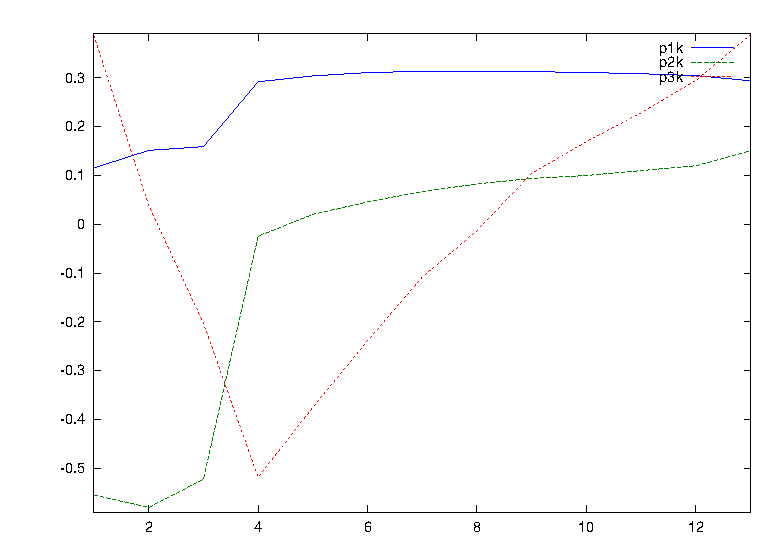
\includegraphics[scale=0.75]{components.eps}
  \caption{Aplikace vektorové analýzy na swapovou křivku Spojených států pro období 03.08.2007 - 03.08.2009. Z grafu je patrné, že $p_{1k}$ je přibližně konstantní, $p_{2k}$, klesající a $p_{3k}$ nejprve rostoucí a následně klesající.}
  \label{components}
\end{figure}
\begin{figure}
  \centering
  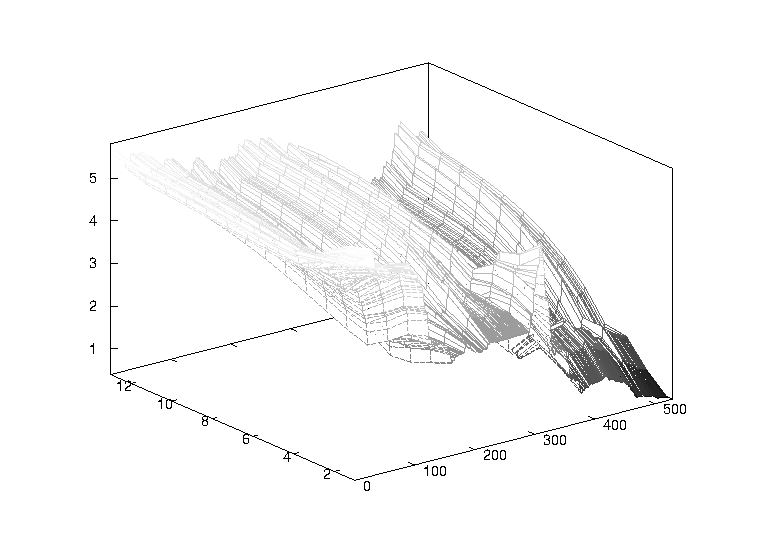
\includegraphics{irs_orig.eps}
  \caption{Původní swapová křivka Spojených států pro období 03.08.2007 - 03.08.2009}
  \label{irs_orig}
\end{figure}
\begin{figure}
  \centering
  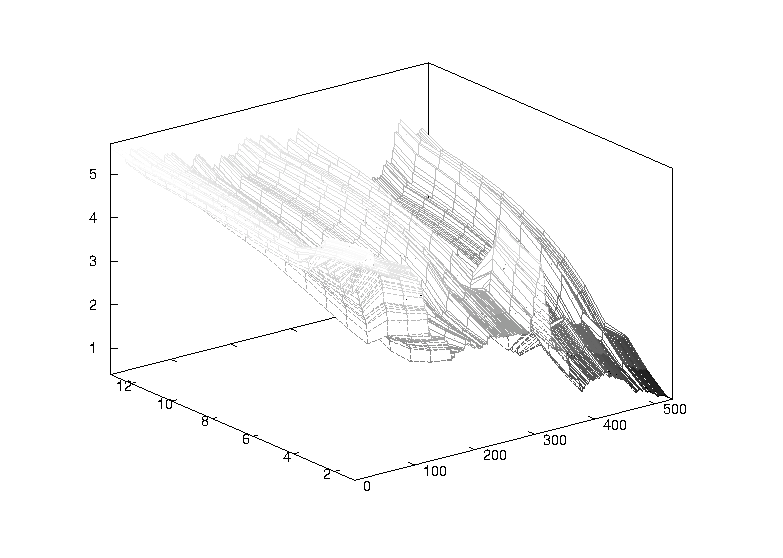
\includegraphics{irs_output.eps}
  \caption{Swapová křivka Spojených států pro období 03.08.2007 - 03.08.2009 po aplikaci vektorové analýzy při využití eigenvektorů $p_{1k}$, $p_{2k}$ a $p_{3k}$}
  \label{irs_output}
\end{figure}
Metoda vektorové dekompozice byla demonstrována na par sazbách swapové křivky Spojených států pro období od 03.08.2007 do 03.08.2009 - viz. obrázky (\ref{components}), (\ref{irs_orig}) a (\ref{irs_output}). Na obrázku (\ref{components}) jsou jednotlivé křivky tvořeny prvky nejvýznamnějších tří eigenvektorů. Všimněme si čtvrtého tenoru. Swapová křivka se skládá z mezibankovních depozitních sazeb, které představují tenory do jednoho roku včetně a swapových sazeb, které představují tenory od dvou let výše. Zmiňovaných čtvrtý tenor představuje jeden rok a je tak předělem mezi depozitním a swapovými sazbami. Změna profilu křivek v tomto tenoru tak indikuje rozdílný tvar swapové křivky do jednoho roku a nad jeden rok, což odpovídá skutečnosti.
\begin{figure}
  \centering
  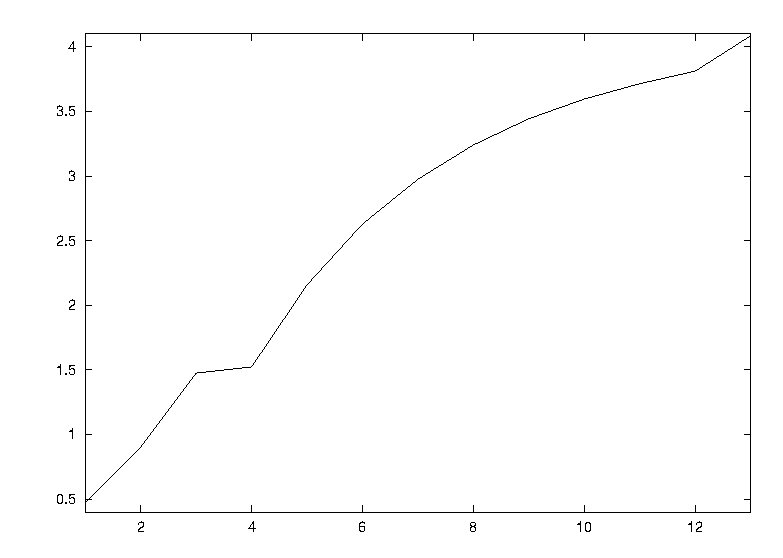
\includegraphics[scale=0.75]{irs_profile.eps}
  \caption{Swapová křivka Spojených států k 03.08.2009 - tenor číslo čtyři odpovídá jednomu roku a představuje tak předěl mezi depozitními a swapovými par sazbami}
  \label{irs_profile}
\end{figure}

Tím, že jsme pro popis změny úrokové sazby použili pouze tři faktory, jsme ztratili část původní informace. První faktor reprezentuje 76.3\% , druhý faktor 17.2\% a třetí faktor 3.4\% celkového rozptylu původní informace. Dohromady tyto faktory představují téměř 97\% rozptylu původní informace.

\section{Klasické teorie časové struktury úrokových sazeb}

Úvahy nad profilem časové struktury úrokových sazeb začínají úvahami o preferencích účastníků trhu. Jestliže by účastníci trhu byli indiferentní mezi krátkodobými a dlouhodobými úrokovými sazbami, byla by úroková křivka plochá. Časová struktura úrokové křivky by tak ztrácela smysl. Ve skutečnosti však účastníci trhu indiferentní ve vztahu k úrokovým sazbám nejsou a jejich preference odráží očekávání, požadovanou rizikovou prémii a v neposlední řadě také povahu jejich aktiv a závazků. Na základě povahy těchto preferencí pak rozlišujeme tři základní teorie, které se snaží vysvětlit časovou strukturu úrokových sazeb.
\begin{itemize}
\item teorii čistého očekávání (pure expectations theory)
\item teorii rizikové prémie
\item teorii oddělených trhů
\end{itemize}
Dále existuje tzv. teorie zkresleného očekávání (biased expectations theory), která kombinuje teorii čístého očekávání a teorii rizikové prémie.

\subsection{Teorie čistého očekáváni}

Podle této teorie odráží časová struktura úrokových sazeb očekávání krátkodobých budoucích úrokových sazeb na trhu. Rostoucí, klesající resp. plochá křivka úrokových sazeb tak indikuje očekávání růstu, poklesu popř. neměnnosti krátkodobých budoucích úrokových sazeb. V rámci této teorie formálně platí
\begin{equation*}
1 + R(t, n) = [(1 + R(t,1))(1 + F^{\alpha}(t, t+1,t))  ... (1 + F^{\alpha}(t, t+n,t))]^{\frac{1}{n}}
\end{equation*}
kde $R(t,n)$ představuje úrokovou sazbu se splatností $n$ roků platnou v čase $t$ a $F^{\alpha}(t, t + k, 1)$ je jednoroční forwardová úrokovou sazba očekávaná trhem v čase $t$ platná od $t + k$ do $t + k +1$.\\

\noindent \textbf{Příklad:} Uvažujme investora s dvouletým investičním horizotem. Předpokládejme, že tento investor má dvě možnosti: (a) uložit finanční prostředky nyní na jeden rok a po roce tuto operaci zopakovat nbo (b) investovat rovnou na dva roky. Protože v rámci teorie čistého očekávání neuvažujeme prémii za riziko ani za likviditu, musí v případě neexistence arbitráže platit
\begin{equation*}
[1 + R(t, 2)]^2 = (1 + R(t,1))(1 + F^{\alpha}(t, t+1,t))
\end{equation*}
Forwardové úrokové sazby tedy reprezentují očekávání trhu. Vzhledem k tomu, že tato očekávání jsou v průměru správná, implikuje teorie čistého očekávání rovnost krátkodobé budoucí úrokové sazby a jí odpovídající krátkodobé forwardové úrokové sazby. Dalším předpokladem této teorie je, že účastnící trhu maximalizují výnos pro svůj investiční horizont a jsou indiferentní mezi dlouhým a krátkým investičním horizontem. $\clubsuit$

\subsection{Teorie rizikové prémie}

V předešlé teorii jsme předpokládáli, že investoři jsou rizikově neutrální a že forwardové sazby jsou dokonalou predikcí budoucích úrokových sazeb. Investoři tak ve snaze maximalizovat výnos v rámci investičního horizontu nemuseli brát v potaz riziko, že skutečné úrokové sazby v budoucnu nebudou rovny současným forwardovým sazbám. Tento předpoklad však v praxi zjevně neplatí, v důsledku čehož jsou s dlouhodobým investičním horizontem spjata určitá rizika. Podle teorie rizikové a likviditní přirážky jsou si investoři tohoto rizika vědomi a požadují kompenzaci za jeho podstoupení. Podle této teorie lze úrokovou sazbu se splatní $n$ roků vyjádřit jako
\begin{equation*}
1 + R(t, n) = [(1 + R(t,1))(1 + L_2)  ... (1 + L_n)]^{\frac{1}{n}}
\end{equation*}
kde $L_i$ představuje rizikovou prémii v $i$-tém roce. Pro rizikovou prémii platí
\begin{equation*}
0 < L_1 < L_2 < ... < L_n
\end{equation*}
a
\begin{equation*}
L_2 > L_3 - L_2 > L_4 - L_3 > ... > L_n - L_{n-1}
\end{equation*}
Vzhledem k tomu, že riziková prémie nemůže být záporná, implikuje teorie rizikové prémie rostoucí křivku úrokových sazeb.\\

\noindent \textbf{Příklad:} Uvažujme investora s dvouletým investičním horizontem. Předpokládejme, že tento investor má dvě možnost: (a) koupit dvouletý státní dluhopis a ten držet do splatnosti nebo (b) koupit desetiletý státní dluhopis a ten po dvou letech prodat. Je zřejmé, že zatímco v prvním případě je investorův výnos předem známý, v druhém případě zavisí na prodejní ceně dluhopisu. Tato cena však není předem známa, protože se bude odvíjet od úrokových sazeb platných za dva roky. Jako kompenzaci za podstupované riziko tak investor požaduje v porovnání s první variantou vyšší očekávaný výnos. $\clubsuit$

\subsection{Teorie oddělených trhů}

Podle teorie oddělených trhů existují skupiny investorů, kteří liší svým investičním horizontem a ovlivňují tak různé segmenty křivky úrokových sazeb. Typickým příkladem jsou banky, které mají krátkodobý až střednědobý investiční horizont a penzijní fondy, které mají naopak dluhodobý investiční horizont. Tvar křivky úrokových sazeb je pak ovlivňován poptávkou a nabídkou pro příslušný segment křivky. Mezi jednotlivými segmenty křivky neexistuje přímá vazba a tak může mít libovolný tvar. 

\subsection{Teorie zkresleného očekávání}

Tato teorie je kombinací teorie čistého očekávání a teorie rizikové prémie. Tvar křivky úrokových sazeb je tak determinován nejen očekávanými budoucími úrokovými sazbami ale také rizikovou prémií, která se může lišit pro jednotlivé splatnosti.
\begin{equation*}
1 + R(t, n) = [(1 + R(t,1))(1 + F^{\alpha}(t, t+1,t) + L_2)  ... (1 + F^{\alpha}(t, t+n,t) + L_3)]^{\frac{1}{n}}
\end{equation*}
Pro likviditní prémii opět platí
\begin{equation*}
0 < L_1 < L_2 < ... < L_n
\end{equation*}
a
\begin{equation*}
L_2 > L_3 - L_2 > L_4 - L_3 > ... > L_n - L_{n-1}
\end{equation*}

\section{Příloha A: Vektorová dekompozice}

\subsection{Eigenvalue a eigenvektory}

Nezbytným předstupněm pro pochopení vektorové analýzy jsou lineární transformace, eigenhodnoty a eigenvektory. Proto se v této kapitole zaměříme na vysvětlení těchto pojmů.

Lineární transformace vektorového prostoru může být vizualizována prostřednictvím efektu, který má na vektory. Lineární transformaci lze tedy chápat jako vektorovou funkci, která mění délku a směr vektorů.

Dle formální definice je vektorová funkce $P$ definována pro vektorový prostor $L$, pokud pro každý nenulový vektor $x$ tohoto vektorového prostoru existuje jedinečné přiřazení $y = Px$. Vektorová funkce $P$ je lineární, pokud splňuje (a) podmínku aditivity $P(x + y) = Px + Py$ a (b) podmínku homogenity $P(\alpha x) = \alpha (Px)$, kde $x$ a $y$ představují libovolné vektory z vektorového prostoru $L$ a $\alpha $ je skalární veličina. O funkci $P$ pak hovoříme jako o lineární transformaci.

Jestliže máme lineární transformaci $P$, je nenulový vektor $x$ definován jako tzv. eigenvektor (eigenvector) transformace, pokud splňuje rovnici
\begin{equation}
Px = \lambda I x
\end{equation}
pro skalární veličinu $\lambda$. Skalární veličinu $\lambda$ nazýváme eigenhodnotou (eigenvalue) odpovídající eigenvektoru $x$ funkce $P$. Hlavní myšlenkou výše uvedené rovnice je, že směr vektoru $x$ není lineární transformací změněn\footnote{V rámci transformace však může dojít ke změně znaménka směru vektoru. V tomto případě hovoříme o tzv. reflexi.}, ale je změněna jeho velikost podle $\lambda$. Většina vektorů tuto podmínku nesplňuje a funkce $P$ změní nejen jejich velikost ale také směr. Pouze některé vektory tak mohou být eigenvektory a pouze některé skalární veličiny mohou být eigenhodnotou.

Rovnici (3.1) lze upravit do tvaru
\begin{equation*}
(P - \lambda I)x = 0
\end{equation*}
V případě, že by existovala inverze $(P - \lambda I)^{-1}$, bylo by možné obě strany rovnice vynásobit touto inverzí a získat tak triviální řešení $x = 0$. Eigenvektorem však může být pouze nenulový vektor. Tato podmínka je splněna, pokud uvažovaná inverze neexistuje, tj. pro $det(P - \lambda I) = 0$. Rovnice $det(P - \lambda I) = 0$ je nazývána charakteristickou rovnicí. Rozvojem charakteristické rovnice získáme polynom $n$-tého řádu. Jeho řešením získáme hodnoty pro jednotlivá $\lambda$. Eigenvektory $x$ nejsou v charakteristické rovnici obsaženy a je třeba je zpětně dopočítat z rovnice (3.1) pro jednotlivé eigenhodnoty.\\

\noindent \textbf{Příklad:} Uvažujme transformační matici
\begin{equation*}
     P =
     \begin{bmatrix}
          1 & 0.92593 \\
          0.92593 & 1
     \end{bmatrix}
\end{equation*}
V prvním kroce vypočteme eigenhodnoty, které jsou řešením rovnice
\begin{equation*}
det(P - \lambda I) = 0
\end{equation*}
\begin{equation*}
     \begin{vmatrix}
          1 - \lambda & 0.92593 \\
          0.92593 & 1 - \lambda
     \end{vmatrix}
     = 0
\end{equation*}
\begin{equation*}
(1 - \lambda)^2 - 0.92593^2 = 0
\end{equation*}
Kořeny kvadratické rovnice jsou $\lambda_1 = 1.92593$ a $\lambda_2 = 0.07407$. Nyní je třeba zpětným dosazením jednotlivých eigenhodnot do eigenrovnice $Px = \lambda x$ dopočíst jednotlivé eigenvektory. V případě eigenhodnoty 1.92593 a transformační matice $P$ má eigenrovnice tvar
\begin{equation*}
     \begin{bmatrix}
          1 & 1.92593 \\
          1.92593 & 1
     \end{bmatrix}
	\begin{bmatrix}
		x_{11} \\
		x_{21}
     \end{bmatrix}
     =
     \lambda
	\begin{bmatrix}
		x_{11} \\
		x_{21}
     \end{bmatrix}     
\end{equation*}
Tato rovnice je splněna pro všechny eigenvektory, pro které platí $x_{21} = x_{11}$. Jako zástupce zvolme eigenvektor jednotkové délky $\begin{bmatrix} 0.7071\\ 0.7071 \end{bmatrix}$. V případě eigenvalue 0.07407 lze analogicky odvodit vztah $x_{21} = -x_{11}$ a eigenvektor $\begin{bmatrix} -0.7071\\ 0.7071 \end{bmatrix}$. Na první pohled je zřejmé, že se jedná o vzájemně kolmé eigenvektory. $\clubsuit$

\subsection{Vektorová dekompozice}

Hlavní myšlenkou vektorové dekompozice (PCA - Principal Component Analysis) je redukce dimenze vstupních dat na základě jejich vzájemné podobnosti. Tato statistická metoda je nejčastěji používána při analýze fyzikálních měření, zpracování obrazu ale také v ekonomii. Pomocí vektorové dekompozice je možné odhalit mezi daty vzájemné souvislosti, které nejsou na první pohled patrné.

Uvažujme lineární transformaci
\begin{equation}
Y = PX
\end{equation}
kde matice $X$ a $Y$ jsou typu $n \times m$ a $P$ je čtvercová matice typu $n \times n$.

Matici vstupních dat $X$ lze chápat jako matici, jejíž řádky představují náhodné veličiny a každý ze sloupců je realizací příslušné náhodné veličiny. Typicky jsou vstupní data představována výsledky měření. Předpokládejme, že se v rámci fyzikálního měření soustředíme na $n$ veličin, které monitorujeme v $m$ časových okamžicích. Výsledkem měření je $n \cdot m$ hodnot, které lze uspořádat do matice typu $n \times m$. Jako příklad uvažujme měření, kdy v jeden časový okamžik měříme teplotu a tlak plynu v uzavřené nádobě. Toto měření opakujme stokrát. Výsledky měření jsme schopni vyjádřit jako matici $n \times m$ popř. vizualizovat ve dvourozměrném prostoru pomocí $m$ bodů. Matice $Y$ představuje analogicky výstupní data lineární transformace.

Vstupní data mohou být vzájemně korelovaná. To znamená, že jejich kovarianční matice $C_X$ je symetrickou maticí s nenulovými prvky mimo diagonálu. Vhodnou volbou transformační matice $P$ lze tuto korelaci ve výstupní matici $Y$ odstranit. Kovarianční matice výstupních dat $C_Y$ je tak diagonální maticí.

Představme si jednotlivé sloupce matice $X$ jako body v $n$ rozměrném prostoru. Celou matici je tak možné interpretovat jako množinu $m$ bodů. Pozice každého bodu je vyjadřována relativně ke zvolenému počátku a osám, které tvoří bázi uvažovaného $n$ rozměrného prostoru. Lineární transformaci (3.2) a s ní spojené odstranění korelací lze chápat jako změnu bázu popř. natočení os ve směru největší informace. Situaci ilustrují obrázky (\ref{data_adj}) a (\ref{data_adj_axis}).
\begin{figure}
  \centering
  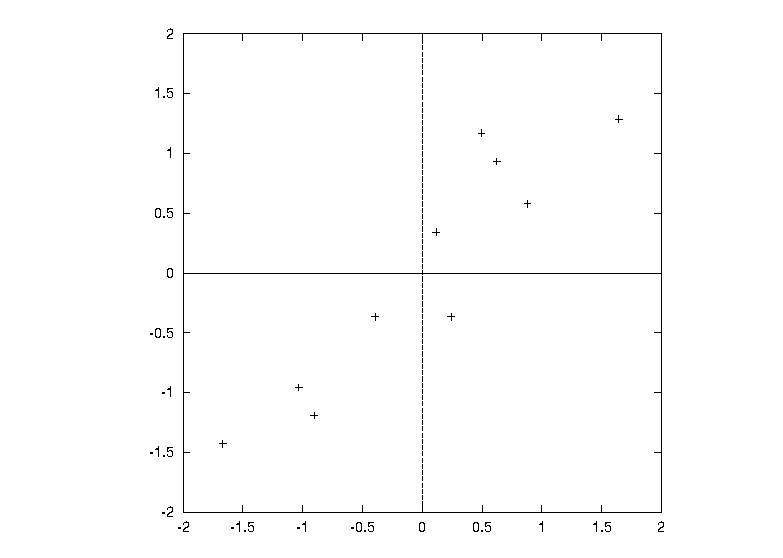
\includegraphics{data_adj.eps}
  \caption{Vizualizace matice $X$ typu $2 \times 10$ ve dvourozměrném prostoru při standardním natočení os}
  \label{data_adj}
\end{figure}
\begin{figure}
  \centering
  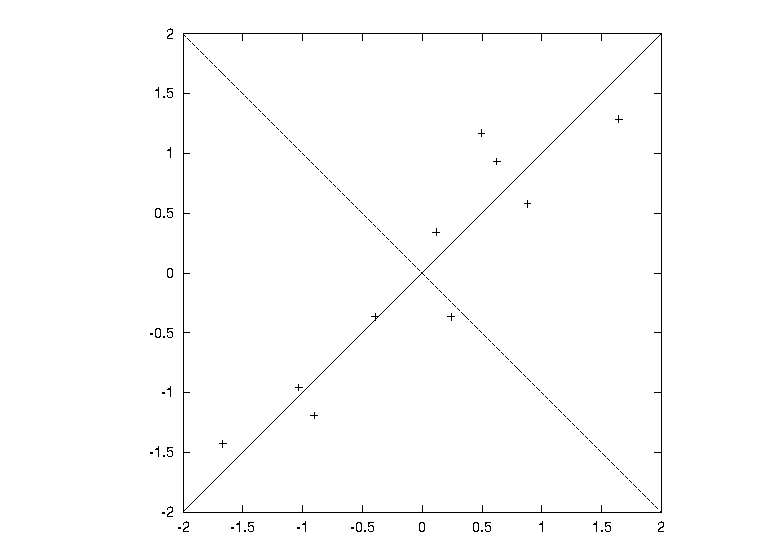
\includegraphics{data_adj_axis.eps}
  \caption{Vizualizace matice $X$ typu $2 \times 10$ ve dvourozměrném prostoru při natočení os ve směru největší informace}
  \label{data_adj_axis}
\end{figure}
Indikátorem míry informace je rozptyl. V obrázku (\ref{data_adj_axis}) došlo k natočení os tak, aby byl rozpyl maximalizován kolem osy procházející levým dolním rohem grafu. Tato osa tak představuje přímku, která nejlépe vystihuje rozložení bodů v rovině. Druhá osa procházející levým horním rohem na sebe váže zbytek rozptylu. 


Lze dokázat, že odstranění korelací ve výstupních datech představovaných maticí $Y$ dosáhneme, pokud řádky transformační matice $P$ budou tvořit eigenvektory korelační matice $C_X$.

\begin{equation*}
C_Y = \frac{1}{n}YY^T
\end{equation*}
\begin{equation*}
C_Y = \frac{1}{n}(PX)(PX)^T
\end{equation*}
\begin{equation*}
\frac{1}{n}PXX^TP^T
\end{equation*}
\begin{equation*}
P\Big(\frac{1}{n}XX^T \Big)P^T
\end{equation*}
\begin{equation*}
C_Y = P C_X P^T
\end{equation*}
V prvním mezikroku jsme prokázali, že kovarianční matici $C_Y$ je možné vyjádřit pomocí kovarianční matice $C_X$ a transformační matice $P$. V dalším kroce použijeme poznatek, že symetrická matice $A$ může být vyjádřena pomocí diagonální matice $D$ a maticí $E$ svých eigenvektorů uspořádaných do sloupců jako $A = EDE^T$.
\begin{equation*}
C_Y = PC_XP^T
\end{equation*}
\begin{equation*}
C_Y = P(EDE^T)P^T
\end{equation*}
Pro matici $P$ platí $P = E^T$ a $P^{-1} = P^T$. Výše odvozený vztah lze tedy dále upravit do podoby
\begin{equation*}
C_Y = P(EDE^T)P^T
\end{equation*}
\begin{equation*}
C_Y = (PP^T)D(PP^T)
\end{equation*}
\begin{equation*}
C_Y = IDI
\end{equation*}
\begin{equation*}
C_Y = D
\end{equation*}
Tímto jsme dokázali, že použijeme-li jako transformační matici $P$ , jejíž řádky budou tvořeny eigenvektory kovarianční matice $C_X$, odstraníme korelaci mezi výstupními daty lineární transformace (3.2). To je cílem vektorové dekompozice.

Uvažujme vektorový prostor $L$ dimenze $n$, jehož bázi tvoří $n$ ortogonálních vektorů společně s nulovým vektorem. Nechť mají všechny nenulové vektory báze jednotkovou délku. Libovolný vektor $v$ z vektorového prostoru $L$ lze vyjádřit ve tvaru
\begin{equation}
v = \sum_{i=1}^n \alpha_i p_i 
\end{equation}
kde $\alpha_i$ představuje skalární veličinu a $p_i$ nenulový vektor báze vektorového prostoru $L$. Předpokládejme, že transformační matice $P$ je tvořena eigenvektory kovarianční matice $C_X$ uspořádaných do řádků a seřazených sestupně podle odpovídajících eigenhodnot\footnote{To znamená, že první řadek matice $P$ tvoří eigenvektor s nejvyšší eigenhodnotou.}. Dále uvažujme vektor $Y_1$, který je tvořen prvním sloupcem matice $Y$ výstupních dat lineární transformace (3.2). Platí
\begin{equation*}
P^TY_1 =
\begin{bmatrix}
p^1_1 & \dots & p^n_1 \\
\vdots & \ddots & \vdots \\
p^1_n & \dots & p^n_n \\
\end{bmatrix}
\begin{bmatrix}
y_{11} \\
\vdots \\
y_{n1} \\
\end{bmatrix}
=
\begin{bmatrix}
p^1_1 y_{11} + \dots + p^n_1 y_{n1} \\
\vdots \\
p^1_n y_{11} + \dots + p^n_n y_{n1} \\
\end{bmatrix}
=
\end{equation*}
\begin{equation}
=
y_{11} \begin{bmatrix} p^1_1 \\ \vdots \\ p^1_n \end{bmatrix}
+
\dots
+
y_{n1} \begin{bmatrix} p^n_1 \\ \vdots \\ p^n_n \end{bmatrix}
=
\sum_{i = 1}^n y_{i1} \begin{bmatrix} p^i_1 \\ \vdots \\ p^i_n \end{bmatrix} = \sum_{i = 1}^n y_{i1} p^i
\end{equation}
Pokud bychom namísto matice $Y_1$ uvažovali matici $Y$, aplikovali bychom analogický postup.

Vztah (3.4) je totožný s (3.3), tj. provedli jsme dekompozici $Y_1$ na vážený součet bazických vektorů. Každý sčítanec představuje kontribuci příslušného bazického vektoru do $Y_1$. Protože jsme v matici $P$ uspořádali eigenvektory sestupně podle eigenhodnoty, jsou sčítanci v (3.4) taktéž seřazeni sestupně. Navíc je rozložení informace mezi jednotlivé sčítance optimální. To znamená, že pokud bychom namísto $P$ použili alternativní bázi $P^*$, platí pro každého sčítance
\begin{equation*}
y_{i1}p^i \ge y_{i1}p^{*i}
\end{equation*} 
Jestliže byla vstupní data představovaná maticí $X$ vzájemně korelována, je kontribuce posledních sčítanců v (3.4) zanedbatelná. To znamená, že jsem schopni snížit dimezi problému za cenu přijatelné ztráty informace. Sumu (3.4) je tak možné vyjádřit jako
\begin{equation*}
\sum_{i = 1}^n y_{i1} p^i = \sum_{i = 1}^{n^*} y_{i1} p^i + \varepsilon \approx \sum_{i = 1}^{n^*} y_{i1} p^i
\end{equation*}
kde $n^* < n$ a $\varepsilon$ je zanedbatelné. Zanedbání posledních $n-n^*$ sčítanců v (3.4) odpovídá redukci matice $P$ a $Y$, kdy použijeme matici $P^*$ typu $n^* \times n$ a matici $Y^*$ typu $n^* \times m$. Pokud si uvědomíme, že
\begin{equation*}
X = P^T Y
\end{equation*}
pak rovnice
\begin{equation}
X^* = P^{*T} Y^*
\end{equation}
vyjadřuje klíčovou myšlenku vektorové dekompozice. V rovnici (3.5) jsme popsali vstupní data reprezentovaná maticí $X$ typu $n \times m$ pomocí matice $Y^*$ typu $n^* \times m$.

Protože $n^* < n$, došlo k snížení dimenze problému. Cenou za snížení dimenze je však ztráta části původní informace, kterou vyjadřujeme ve formě snížení rozptylu jako
\begin{equation*}
I_{loss} = 1 - \frac{\sum_{i = 1}^{n^*}\lambda_i}{n}
\end{equation*}
kde $\lambda_i$ představuje eigenhodnotu $i$-tého nejvýznamnějšího eigenvektoru. Kontribuci $i$-tého eigenvektru v procentech k celkovému rozptylu lze tedy vyjádřit
\begin{equation*}
C_i = \frac{\lambda_i}{n}
\end{equation*}
\begin{figure}
  \centering
  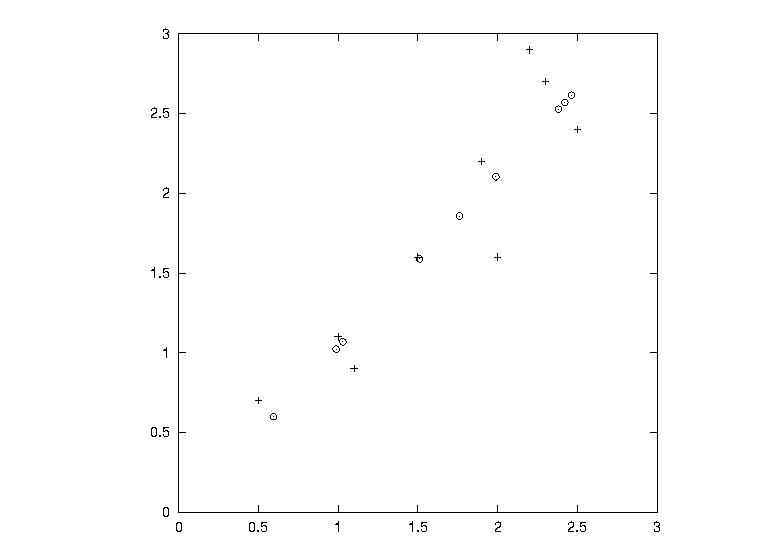
\includegraphics{data.eps}
  \caption{Snížení dimenze problému pomocí vektorové dekompozice - původní data jsou představována křížky, data po snížení dimenze problému o jeden řád jsou představována kolečky}
  \label{data}
\end{figure}

\noindent \textbf{Příklad:} Uvažujme dvě náhodné veličiny $x$ a $y$. Realizace těchto náhodných veličin zachycuje následující tabulka.
\begin{center}
     \begin{tabular}{c | c}
     $x$ & $y$ \\
     \hline
     2.5 & 2.4 \\
     0.5 & 2.9 \\
     1.9 & 2.2 \\
     3.1 & 3.0 \\
     2.3 & 2.7 \\
     2.0 & 1.6 \\
     1.0 & 1.1 \\
     1.5 & 1.6 \\
     1.1 & 0.9 \\
     \end{tabular}
\end{center}
Pro správné fungování vektorové dekompozice je důležité provést normolizaci vstupních dat. V případě náhodné veličiny $x$ se normalizace provede podle rovnice
\begin{equation*}
\dot{x}_i = \frac{x_i - \bar{x}}{\sigma_x}
\end{equation*}
kde $\bar{x}$ představuje aritmetický průměr a $\sigma_x$ směrodatnou odchylku náhodné veličiny $x$. Pro náhodnou veličinu $y$ je postup analogický. Normalizováním vstupních dat získáme matici $X$
\begin{equation*}
     X =
     \begin{bmatrix}
     0.879 & -1.668 & 0.497 & 0.115 & 1.643 & 0.624 & 0.242 & -1.032 & -0.398 & -0.904 \\
     0.579 & -1.429 & 1.170 & 0.343 & 1.288 & 0.933 & 0.366 & -0.957 & -0.366 & -1.193 \\
     \end{bmatrix}
\end{equation*}
kde první řádek představuje hodnoty $\dot{x}$ a druhý řádek hodnoty $\dot{y}$. Dalším krokem je výpočet kovarianční matice $C_X$ pro $\dot{x}$ a $\dot{y}$
\begin{equation*}
C_X = \frac{1}{n-1}XX^T
\end{equation*}
kde $n$ představuje počet řádek matice $X$\footnote{V teoretické části této kapitoly jsme vypočetli kovarianční matici jako $\frac{1}{n}XX^T$. Důvod, proč je nyní namísto $n$ aplikujeme $n-1$, je ten, že počítáme tzv. výběrovou kovarianci. Vysvětlení lze nalézt v teorii výběru.}. V našem konkrétním případě je kovarianční matice rovna
\begin{equation*}
C_X =
     \begin{bmatrix}
          1.00000 & 0.92593 \\
          0.92593 & 1.00000
     \end{bmatrix}
\end{equation*}
Eigenhodnoty a eigenvektory kovarianční matice $C_X$ jsme vypočetli v předchozí kapitole. Nechť $P$ je maticí eigenvektorů, kde jednotlivé eigenvektory tvoří řádky matice a nechť jsou tyto eigenvektory seřazeny sestupně podle své eigenhodnoty. V prvním řádku je tak eigenvektor s nejvyšší eigenhodnotou, v druhém sloupci eigenvektor s druhou nejvyšší eigenhodnotou atd.
\begin{equation*}
P =
     \begin{bmatrix}
          0.7071 & 0.7071 \\
          0.7071 & -0.7071
     \end{bmatrix}
\end{equation*}

Uvažujme matici $Y$
\begin{equation*}
Y = PX
\end{equation*}
která představuje výstupní data lineární transformace. Pokud bychom aplikovali rovnici $X = P^TY$, dopočetli bychom zpětně matici vstupních dat $X$. Pokud však snížíme dimenzi problému o jeden řád a použijeme rovnici (3.5), získáme matici $X^*$.
Po vynásobení matice $X^*$ směrodatnou odchylkou a přičtení aritmetickéh průměru náhodné veličiny $x$ resp. $y$, získáme vstupní data ve zredukované podobě.
\begin{center}
     \begin{tabular}{c | c}
     $x^*$ & $y^*$ \\
     \hline
	2.38226 & 2.52693 \\
	0.59380 & 0.59888 \\
	2.46416 & 2.61522 \\
	1.98950 & 2.10351 \\
	2.96054 & 3.15034 \\
	2.42140 & 2.56912 \\
	1.76122 & 1.85741 \\
	1.02932 & 1.06839 \\
	1.51122 & 1.58790 \\
	0.98656 & 1.02229 \\
    \end{tabular}
\end{center}
Vztah mezi původními vstupními daty a daty po zredukování dimenze zobrazuje obrázek (\ref{data}).

Protože eigenhodnota použitého eigenvektoru je rovna 1.92593, ztratili jsem v rámci vektorové dekompozice informaci, která odpovídá necelým čtyřem procentům celkového rozptylu.
\begin{equation*}
1 - \frac{1.92593}{2} = 3.7\%
\end{equation*}
\noindent $\clubsuit$

\chapter{Odvození zero křivky}

Připomeňme, že zero křivka je křivka, která se skládá z tzv. zero sazeb. Aktuální zero sazbu platnou pro čas $t$ lze chápat jako cenu diskontního dluhopisu se splatností v čase $t$. Pomocí zero křivky můžeme
\begin{itemize}
\item dopočíst dikontní faktory a následně cenu libovolného finančního instrumentu s fixním cash-flow
\item odvodit implikované křivky jakou je např. forwardová úroková křivka
\end{itemize}

\section{Odvození zero křivky pro státní dluhopisy}

\subsection{Výběr dluhopisů}

Pro odvození zero křivky státních dluhopisů vybíráme dluhopisy s deterministickým cash-flow emitované centrální vládou v její domácí měně. Dalším významným faktorem pro výběr dluhopisů je jejich likvidita - vybrané dluhopisy musí být likvidní avšak nesmí být přespříliš exponované\footnote{Pojmem exponovaný dluhopis označujeme dluhopis, jehož cena může být zkreslena nadměrnou poptávkou. Typickým příkladem jsou tzv. benchmarkové dluhopisy popř. dluhopisy, které tvoří podklad pro dluhopisové futures a v době jejich splatnosti jsou cheapest-to-deliver. Cena tohoto dluhopisu tak může být zkreslena z titulu nadměrné poptávky.}. Dále je důležité vybrat dluhopisy tak, aby byly uspokojivě pokryty všechny segmenty konstruované křivky.

\subsection{Přímá metoda konstrukce křivky}

\subsubsection{Teoretický přístup}

Předpokládejme, že potřebujeme zkonstruovat zero křivku, která se skládá z $n$ zero sazeb se splatnostmi jeden, dva až $n$ roků. Nejprve je třeba vybrat $n$ fixních popř. diskontních dluhopisů s odpovídající zbytkovou splatností. Vektorem
\begin{equation*}
P_t = [P_t^1, P_t^2, ..., P_t^n]^T
\end{equation*}
rozumnějme vektor cen těchto dluhopisů v čase $t$. Nechť všechny dluhopisy generují cash-flow vždy ke stejným datům $t_i$, kde $i = 1, ..., n$. Cash-flow uvažovaných dluhopisů je tak možné uspořádat do matice typu $n \times n$.
\begin{equation*}
F = \begin{bmatrix} F^1_1 & F^1_2 & ... & F^1_n \\ F^2_1 & F^2_2 & ... & F^2_n \\ \dots \\ F^n_1 & F^n_2 & ... & F^n_n \end{bmatrix}
\end{equation*}
Dále uvažujme matici vektor $B_t$ diskontních faktorů
\begin{equation*}
B_t = [B(t, t_1), ..., B(t, t_n)]^T
\end{equation*}
Je zřejmé, že v případě neexistence arbitráže musí pro $j$-tý dluhopis platit
\begin{equation*}
P_t^j = \sum_{i=1}^n F^j_{t_i} B(t, t_i)
\end{equation*}
Ekvivalentně v maticovém vyjádření pro všechny dluhopisy platí
\begin{equation*}
P_t = F \cdot B_t
\end{equation*}
Vektor diskontních faktorů $B_t$ je tak možné, za předpokladu existence inverzní matice k matici $F$, vyjádřit jako
\begin{equation*}
B_t = F^{-1} P_t
\end{equation*}
Tímto jsme tedy vypočetli matici implikovaných cen diskotnotních dluhopisů, které jsou konzistentní s původními tržními cenami. Z těchto cen lze vyjádřit zero sazby s ročním úročením
\begin{equation*}
R(t, t_i - t) = e^{-\frac{1}{t_i - t} \ln[B(t, t_i)]}-1
\end{equation*}
popř. zero sazby se spojitým úročením
\begin{equation*}
R^c(t, t_i - t) = - \frac{1}{t_i - t} \ln[B(t, t_i)]
\end{equation*}
Tato metoda je velmi jednoduchá. Předpoklad, že cash-flow všech dluhopisů se realizuje ve shodné časové okamžiky $t_i$ je však v praxi značně svazující. Proto je v praxi spíše uplatnitelná metoda bootstrapingu.

\subsubsection{Metoda bootstrapingu}

Metoda bootstrapingu je založená na postupné konstrukci zero křivky na základě tržních cen dluhopisu. Metoda výpočtu probíhá v následujících krocích.
\begin{itemize}
\item Vypočteme zero sazby přímo z cen diskontních dluhopisů se zbytkovou splatností menší než jeden rok.
\item Na zero sazby aplikujeme lineární nebo kubickou interpolaci pro sestrojení kontinuální zero křivky.
\item Zvolíme dluhopis se zbytkovou splatností jeden až dva roky. Při roční výplatě kupónů má tento dluhopis dvě cash-flow - jedno se realizuje do jednoho roku a druhé v rozmezí jednoho až dvou let. Diskontní faktor pro první cash-flow známe a druhý diskotní faktor jsme schopni dopočítat z tržní ceny dluhopisu. Z diskontního faktoru vypočteme zero sazbu.
\item Na zero sazby aplikujeme lineární nebo kubickou interpolaci pro sestrojení kontinuální zero křivky na časovém intervalu jeden až dva roky.
\item Výše uvedené dva kroky aplikujeme opakovaně, dokud nesestrojíme celou zero křivku.
\end{itemize}

\subsubsection{Lineární a kubická interpolace}

Předpokládejme, že známe zero sazby $R(0,x)$ a $R(0,z)$ a potřebujeme dopočíst zero sazbu $R(0,y)$, kde $x \le y \le z$. S pomocí lineární interpolace lze $R(0,y)$ vyjádřit jako
\begin{equation*}
R(0,y) = \frac{(z-y)R(0,x) + (y - x)R(0,z)}{z - x}
\end{equation*}

Pro alikaci kubické interpolace potřebujeme čtyři zero sazby $R(0,v)$, $R(0,x)$, $R(0,y)$ a $R(0,z)$ za podmínky $v < x < y < z$. Interpolovaná zero sazba $R(0,w)$, kde $w \in [v; z]$ je dána polynomem třetího řádu
\begin{equation*}
R(0,w) = aw^3 + bw^2 + cw + d
\end{equation*}
kde $a$, $b$, $c$ a $d$ jsou řešením soustavy rovnic
\begin{equation*}
R(0,v) = av^3 + bv^2 + cv + d
\end{equation*}
\begin{equation*}
R(0,x) = ax^3 + bx^2 + cx + d
\end{equation*}
\begin{equation*}
R(0,y) = ay^3 + by^2 + cy + d
\end{equation*}
\begin{equation*}
R(0,z) = az^3 + bz^2 + cz + d
\end{equation*}
Maticově lze tyto parametry vyjádřit jako
\begin{equation*}
\begin{bmatrix}
a \\ b \\ c \\ d
\end{bmatrix}
=
\begin{bmatrix}
v^3 & v^2 & v & 1 \\
x^3 & x^2 & x & 1 \\
y^3 & y^2 & y & 1 \\
z^3 & z^2 & z & 1
\end{bmatrix}^{-1}
\begin{bmatrix}
R(0, v) \\
R(0, x) \\
R(0, y) \\
R(0, z)
\end{bmatrix}
\end{equation*}
Při konstrukci křivky je kubická interpolace nejprve aplikována na první čtyři zero sazeby odvozené z cen dluhopisů. Tímto způsobem se definují zero sazby mezi těmito body. Poté jsou použity následující čtyři zero sazby pro dopočtení další části zero křivky. Postup se opakuje, dokud není zkonstruována celá křivka.

Výše popsaný postup konstrukce zero křivky pomocí kubické interpolace může mít za následek, že křivka nemusí být hladká. Dále je možné, že takto zkonstruovaná křivka bude konvexní na určitém segmentu a konkávní na jiném.

\subsection{Nepřímá metoda konstrukce křivky}

Nepřímé metody konstrukce výnosové křivky jsou založené na kalibraci vybraného modelu podle třžních dat. Aby aplikace nepřímé metody byla úspěšná, je třeba vybrat vhodný model. Obecný postup aplikace nepřímých metod je následující. Nejprve vyberme $n$ dluhopisů. Cenu $j$-tého dluhopisu v čase $t$ označme jako $P_t^j$ a jeho cash-flow generované v čase $s$ jako $F_s^j$, kde $s \ge t$. Dále definujme funkci diskontního faktoru $B(t,s) \equiv f(s - t, \beta_1)$ popř. funkci zero sazby $R(t,s - t) \equiv g(s - t, \beta_2)$, kde $\beta_1$ a $\beta_2$ jsou vektory zatím blíže nespecifikovaných parametrů.

Funkce $f$ je zpravidla definovaná po částech jako polynomická, exponenciální nebo B-segmentová funkce. Cílem je umožnit aplikaci rozdílných parametrů pro rozdílné segmenty křivky. Funkce $g$ je obvykle definovaná tak, aby její parametry měly jednoduchou ekonomickou interpretaci.

V rámci nepřímé metody jsou odhadnuty parametry $\hat{\beta}$ tak, aby modelové ceny dluhopisů co nejpřesněji kopírovali ceny tržní. Parametry $\hat{\beta}$ jsou tak řešením optimazační rovnice
\begin{equation}
\hat{\beta} = \arg \underset{\beta}{min} \sum_{j = 1}^n (P_t^j - \hat{P_t^j})
\end{equation}
kde $\hat{P_t^j}$ představuje modelovou cenu vypočtenou podle
\begin{equation*}
\hat{P_t^j} = \sum_s F_s^j f(s - t; \beta)
\end{equation*}
popř.
\begin{equation*}
\hat{P_t^j} = \sum_s F_s^j e^{-(s - t)g(s - t; \beta)}
\end{equation*}

V následujícím textu budeme používat níže uvedené značení.
\begin{center}
\begin{tabular}{l l}
$n$ & počet dluhopisů použitých pro odhad výnosové křivky \\
$P_t^j$ & tržní cena $j$-tého dluhopisu v čase $t$ \\
$\hat{P_t^j}$ & teoretická cena $j$-tého dluhopisu v čase $t$ vypočtená dle modelu \\
$P_t$ & vektor tržních cen referenčních dluhopisů v čase $t$ \\
$\hat{P_t}$ & vektor teorických cen referenčních dluhopisů v čase $t$ \\
$T_j$ & zbytková splatnost $j$-tého dluhopisu \\
$F_s^j$ & cash-flow generované $j$-tým dluhopisem v čase $s \ge t$ \\
$B(t,s)$ & diskontní faktor (cena diskontního dluhopisu v čase $t$ se splatností v čase $s$) \\ 
\end{tabular}
\end{center}
Za předpokladu neexistence arbitráže musí platit
\begin{equation*}
\hat{P_t^j} = \sum_{\substack{s = T_i - \alpha_j + 1 \\ s > 0}} F_s^j B(t,s)
\end{equation*}
Model je vyjádřen jako
\begin{equation*}
P_t = \hat{P_t} + \varepsilon
\end{equation*}
kde rezidua $\varepsilon$ pro $\forall(j, j') \in \{1, ..., n\}^2$ splňují podmínky
\begin{equation*}
E[\varepsilon_j] = 0
\end{equation*}
\begin{equation*}
D[\varepsilon_j] = \sigma^2 w_j^2
\end{equation*}
\begin{equation*}
cov[\varepsilon_j, \varepsilon_{j'}] = 0, j \neq j'
\end{equation*}
Kovarianční matice reziduí je tak $\sigma^2 \Omega$ pro $\sigma \in R^+$, kde
\begin{equation*}
\Omega =
\begin{bmatrix}
w_1^2 & 0 & \dots & 0 \\
0 & w_2^2 & & \vdots \\
\vdots & & \ddots & 0 \\
0 & \dots & 0 & w_n^2 \\
\end{bmatrix}
\end{equation*}
Specifikace $w_j^2$ je kritickým bodem celé procedury. Tento člen totiž představuje váhu jednotlivých dluhopisů v optimalizační rovnici (4.1). Řada autorů jednoduše uvažuje homoskedastický případ, kdy
\begin{equation*}
w_j^2 \equiv 1 ~~~ \forall j \in \{1, ..., n\} 
\end{equation*}
a všechny dluhopisy tak mají shodnou váhu. V tomto případě však krátký konec křivky odpovídá skutečným tržním datům pouze přibližně. Ve snaze napravit tento nedostatek, navrhli v roce 1982 Vašíček a Fong zvýšit váhu krátkých dluhopisů a definovali $w_j^2$ jako
\begin{equation*}
w_j^2 = \Bigg( \frac{d P_t^j}{dy_j(t)} \Bigg) = \frac{D_j^2(t)P_t^j}{(1 + y_j(t))^2}
\end{equation*}
kde $y_j(t)$ přestavuje výnos do splatnosti $j$-tého dluhopisu v čase $t$ a $D_j(t)$ je durace $j$-tého dluhopisu v čase $t$. Logika tohoto přístupu vychází z předpokladu, že ocenění dlouhodobých dluhopisů je obtížnější než ocenění dluhopisů se zbytkovou splatností kratší než jeden rok, k jejich ocenění je třeba pouze jedna zero sazba.

Vedle výše uvedeného značení definujme
\begin{center}
\begin{tabular}{l l}
$\beta$ & vektor parametrů pro odhadovanou diskontní funkci\\
$\hat{\beta}$ & odhad vektoru $\beta$\\
$Z$ & matice koeficientů pro každý referenční dluhopis\\
\end{tabular}
\end{center}

\subsubsection{Konstrunkce diskontní křivky}

V této části textu se zaměříme na odhad vektoru $\beta$, který je tvořen parametry modelu diskontní křivky. Model budeme kalibrovat podle tržních hodnot vybraných státních dluhopisů. Pro modelování diskontní křivky použijeme segmentové funkce. Z diskotní křivky lze následně snadno odvodit zero sazby.\\

\noindent \textbf{Polynomická segmentová funkce~} Uvažujme diskontní funkci, která se skládá ze tří segmentových funkcí představovaných polynomy třetího řádu\footnote{Modelová křivka diskontních faktorů se může teoreticky skládat z libovolného množství segmentových funkcí představovaných polynomy libovolného řádu. V praxi se však nejvíce osvědčil námi uvažovaný příklad.}.
\begin{equation}
B(0,s) =
\begin{cases}
B_{0}(s) = d_0 + c_0s + b_0s^2 + a_0s^3, ~ s \in \{0,t_0\}\\
B_{t_0}(s) = d_1 + c_1s + b_1s^2 + a_1s^3, ~ s \in \{t_0,t_1\}\\
B_{t_1}(s) = d_2 + c_2s + b_2s^2 + a_2s^3, ~ s \in \{t_1,t_2\}
\end{cases}
\end{equation}
Parametry $t_0$, $t_1$ a $t_2$ jsou zvoleny s ohledem na tvar křivky a platí pro ně $t_0 \le t_1 \le t_2$. Interval $\{0, t_0\}$ pokrývá krátký konec, interval $\{t_0, t_1\}$ střed a interval $\{t_1, t_2\}$ dlouhý konec diskontní křivky. Diskontní funkce musí dále splňovat podmínky
\begin{gather}
B_{0}(0) = 1 \\
B_{0}^{(i)}(t_0) = B_{t_0}^{(i)}(t_0) \\
B_{t_0}^{(i)}(t_1) = B_{t_1}^{(i)}(t_1)
\end{gather}
kde $B^{i}$ představuje $i$-tou derivaci funkce $B(\cdot)$ pro $i = 0, 1, 2$ podle $s$. Logika podmínky (4.3) vycházející z časové hodnoty peněz je zřejmá - hodnota cash-flow vypláceného v současnosti je rovna jeho nominální hodnotě. Zbývající dvě podmínky vychází z požadavku na spojitost křivky. Po zohlednění těchto podmínek přejde funkce diskontní křivky do tvaru
\begin{equation*}
B(0,s) =
\begin{cases}
B_{0}(s) = 1 + c_0s + b_0s^2 + a_0s^3, ~ s \in \{0,t_0\}\\
B_{t_0}(s) = 1 + c_0s + b_0s^2 + a_0[s^3 - (s - t_0)^3] + a_1(s - t_0)^3, ~ s \in \{t_0,t_1\}\\
\begin{split} B_{t_1}(s) = 1 + c_0s + b_0s^2 + a_0[s^3 - (s - t_0)^3]  + a_1[(s - t_0)^3 - (s - t_1)^3]\\ + a_2(s - t_1)^3, ~ s \in \{t_1,t_2\} \end{split}
\end{cases}
\end{equation*}
S využitím funkce $(s - t_i)_{+} = \max(s - t_i, 0)$ lze tyto rovnice upravit na
\begin{equation}
\begin{split}
B(0,s) = 1 + c_0s + b_0s^2 + a_0s^3 + (a_1 - a_0)(s - t_0)_{+}^3 \\
+ (a_2 - a_1)(s - t_1)_{+}^3, ~ s \in \{0, t_2\}
\end{split}
\end{equation}
Původní počet dvanácti parametrů v rovnici (4.2) tak byl zredukován na pět.\\

\noindent \textbf{Exponenciální segmentová funkce~} Exponenciální segmentové funkce byly prvně při konstrukci diskontní křivky použity Vašíčkem a Fongem v roce 1982.

Uvažujme diskontní křivku, která se skládá z exponenciálních segmentových funkcí a má tvar
\begin{equation}
B(0,s) =
\begin{cases}
B_{0}(s) = d_0 + c_0e^{-us} + b_0e^{-2us} + a_0e^{-3us}, ~ s \in \{0,t_0\}\\
B_{t_0}(s) = d_1 + c_1e^{-us} + b_1e^{-2us} + a_1e^{-3us}, ~ s \in \{t_0,t_1\}\\
B_{t_1}(s) = d_2 + c_2e^{-us} + b_2e^{-2us} + a_2e^{-3us}, ~ s \in \{t_1,t_2\}
\end{cases}
\end{equation}
kde $u < 0$, $t_0 \le t_1 \le t_2$ a která stejně jako v případě polynomické segmentové funkce splňuje podmínky (4.3) až (4.5).

Počet parametrů v segmentové funkci (4.7) lze pomocí těchto podmínek zredukovat z dvanácti na pět\footnote{Parametr $u$, ke kterému se vrátíme později, ponechme prozatím stranou.}. Nejprve zredukujeme počet proměnných ve funkci $B_{t_0}(s)$.
\begin{equation*}
B_0(t_0) = B_{t_0}(t_0) \Leftrightarrow d_1 - d_0 = (c_0 - c_1)e^{-t_0u} + (b_0 - b_1)e^{-2t_0u} + (a_0 - a_1)e^{-3t_0u}
\end{equation*}
\begin{equation*}
B_0^{(1)}(t_0) = B_{t_0}^{(1)}(t_0) \Leftrightarrow c_1 - c_0 = 2(b_0 - b_1)e^{-t_0u} + 3(a_0 - a_1)e^{-2t_0u}
\end{equation*}
\begin{equation*}
B_0^{(2)}(t_0) = B_{t_0}^{(2)}(t_0) \Leftrightarrow c_1 - c_0 = 4(b_0 - b_1)e^{-t_0u} + 9(a_0 - a_1)e^{-2t_0u}
\end{equation*}
Návaznými elementárními operacemi získáme z výše uvedených vztahů
\begin{equation*}
b_1 - b_0 = 3(a_0 - a_1)e^{-t_0u}
\end{equation*}
\begin{equation*}
c_1 - c_0 = -3(a_0 - a_1)e^{-2t_0u}
\end{equation*}
\begin{equation*}
d_1 - d_0 = (a_0 - a_1)e^{-3t_0u}
\end{equation*}
Výsledný tvar segmentové funkce $B_{t_0}(s)$ je tak
\begin{equation*}
B_{t_0}(s) = d_0 + c_0 e^{-us} + b_0e^{-2us} + a_0\Big[e^{-3us} - \Big(e^{-us} - e^{-ut_0} \Big)^3 \Big] + a_1\Big( e^{-us} - e^{-ut_0} \Big)^3
\end{equation*}
Podobně lze zjednodušit také segmentovou funkci $B_{t_1}(s)$.
\begin{equation*}
\begin{split}
B_{t_0}(t_1) = B_{t_1}(t_1) \Leftrightarrow d_2 - d_0 = (c_0 - c_2)e^{-t_1u} + (b_0 - b_2)e^{-2t_1u}\\ + (a_0 - a_2)e^{-3t_1u} + (a_1 - a_2)\Big( e^{-t_1u} - e^{-t_0 u} \Big)^3\\
B_{t_0}^{(1)}(t_1) = B_{t_1}^{(1)}(t_1) \Leftrightarrow c_2 - c_0 = 2(b_0 - b_2)e^{-t_1u} + 3(a_0 - a_2)e^{-2t_1u}\\
+ 3(a_1 - a_0)\Big( e^{-t_1u} - e^{-t_0u} \Big)^2
\end{split}
\end{equation*}
\begin{equation*}
\begin{split}
B_{t_0}^{(2)}(t_1) = B_{t_1}^{(2)}(t_1) \Leftrightarrow c_2 - c_0 = 4(b_0 - b_2)e^{-t_1u} + 9(a_0 - a_2)e^{-2t_1u}\\
+ 3(a_1 - a_0)\Big( e^{-t_1u} - e^{-t_0u} \Big) \Big( 3e^{-t_1u} - e^{-t_0u} \Big)
\end{split}
\end{equation*}
Na základě těchto vztahů lze odvodit
\begin{equation*}
b_2 - b_0 = 3(a_0 - a_2)e^{-t_1u} + 3(a_1 - a_0)\Big( e^{-t_1u} - e^{-t_0u} \Big)
\end{equation*}
\begin{equation*}
c_2 - c_0 = -3(a_0 - a_2)e^{-2t_1u} + 3(a_1 - a_0)\Big( e^{-2t_1u} - e^{-2t_0u} \Big)
\end{equation*}
\begin{equation*}
d_2 - d_0 = (a_0 - a_2)e^{-3t_1u} + (a_1 - a_0)\Big( e^{-3t_0u} - e^{-3t_1u} \Big)
\end{equation*}
Segmentová funkce $B_{t_1}(s)$ má tak podobu
\begin{equation*}
\begin{split}
B_{t_1}(s) = d_0 + c_0e^{-us} + b_0e^{-2us} + a_0 \Big[ e^{-3us} - \Big( e^{-us} - e^{-ut_0} \Big)^3 \Big] \\
+ a_1 \Big[ (e^{-us} - e^{-ut_0})^3 - (e^{-us} - e^{-ut_1})^3 \Big] + a_2 \Big( e^{-us} - e^{-ut_1} \Big)^3
\end{split}
\end{equation*}
Vzhledem k podmínce (4.3) platí $d_0 = 1 - c_0 - b_0 - a_0$. Výsledná podoba diskontní křivky (4.7) je tak
\begin{equation*}
B(0,s) = 
\begin{cases}
B_0(s) = 1 + c_0\Big(e^{-us} - 1 \Big) + b_0 \Big(e^{-2us} - 1 \Big) + a_0 \Big(e^{-3us} - 1 \Big), ~ s \in \{0,t_0\}\\
\begin{split}
B_{t_0}^{(2)}(t_1) = 1 + c_0 \Big( e^{-us} - 1 \Big) + b_0 \Big(e^{-2us} - 1 \Big) + a_0\Big[e^{-3us} - 1 - \Big(e^{-us} - e^{-t_0u} \Big)^3 \Big]\\ + a_1\Big( e^{-us} - e^{-ut_0} \Big)^3, ~ s \in \{t_0,t_1\}
\end{split}
\\
\begin{split}
B_{t_1}(s) = 1 + c_0 \Big(e^{-us} - 1 \Big) + b_0 \Big( e^{-2us} - 1 \Big) + a_0 \Big[ e^{-3us} - 1 - \Big( e^{-us} - e^{-ut_0} \Big)^3  \Big]\\
+ a_1 \Big[ (e^{-us} - e^{-ut_0})^3 - (e^{-us} - e^{-ut_1})^3 \Big] + a_2 \Big( e^{-us} - e^{-ut_1} \Big)^3, ~ s \in \{t_1,t_2\}
\end{split}
\end{cases}
\end{equation*}
Definujme funkci $(e^{-us} - e^{-ut_i})_{-}$ jako $\min(e^{-us} - e^{-ut_i}, 0)$. S její pomocí lze  $B(0,s)$ zredukovat do podoby
\begin{equation}
\begin{split}
B(0,s) = 1 + c_0 \Big( e^{-us} - 1 \Big) + b_0 \Big( e^{-2us} - 1 \Big) + a_0 \Big[ e^{-3us} - 1 - \Big( e^{-us} - e^{-ut_0} \Big)_{-}^3 \Big]\\
+ a_1 \Big[ \Big(e^{-us} - e^{-ut_0} \Big)_{-}^3 - \Big(e^{-us} - e^{-ut_1} \Big)_{-}^3\Big] + a_2 \Big(e^{-us} - e^{-ut_1} \Big)_{-}^3, ~ s \in \{0, t_2 \}
\end{split}
\end{equation}
V rovnici (4.8) figurují parametry $c_0, b_0, a_0, a_1, a_2$, které tvoří vektor $\beta$, a parametr $u$. Tento parametr má zajímavou ekonomickou interpretaci. Vašíček a Fong (1982) dokázali, že
\begin{equation*}
u = \underset{s \rightarrow \infty}{\lim} f(0,s)
\end{equation*}
Na $u$ možné tedy možné pohlížet jako na okamžitou forwardovou sazbu pro nekonečně dlouhý časový horizont.\\

\noindent \textbf{B-segmentová funkce~} B-segmentová funkce je lineární kombinací ohraničených polynomických funkcí. Předpokládejme, že pro účely konstrukce diskontní křivky budeme uvažovat segmenty $(0, t_0)$, $(t_0, t_1)$ a $(t_1, t_2)$. Diskontní křivku lze v tomto případě vyjádřit pomocí B-segmentové funkce jako
\begin{equation}
B(s) = \sum_{i = -3}^2 c_l B_l^3(s) = \sum_{l = -3}^2 c_l \Bigg( \sum_{j=l}^{l + 4} \Bigg[ \prod_{\substack{i=l \\ i \neq j}}^{l+4} \frac{1}{\lambda_i - \lambda_j}\Bigg](s - \lambda_j)_{+}^3\Bigg)
\end{equation}
kde $\lambda_i$ je definováno jako
\begin{equation*}
\lambda_{-3} < \lambda_{-2} < \lambda_{-1} < \lambda_0 = 0 < \lambda_1 = t_0 < \lambda_2 = t_1 < \lambda_3 = t_2 < \lambda_4 < \lambda_5 < \lambda_6
\end{equation*}
Parametry $\lambda_0$, $\lambda_1$, $\lambda_2$ a $\lambda_3$ jsou tzv. uzlové body ohraničující zvolené segmenty zatímco parametry $\lambda_{-3}$, $\lambda_{-2}$, $\lambda_{-1}$, $\lambda_4$, $\lambda_5$ a $\lambda_6$ musí pouze splňovat
\begin{equation*}
\lambda_{-3} < \lambda_{-2} < \lambda_{-1} < 0 < \dots < t_2 < \lambda_4 < \lambda_5 < \lambda_6
\end{equation*}
což je nezbytná matematická podmínka pro existenci B-segmentové funkce $B_l^3(\theta)$. Bázi B-segmentové funkce tvoří vektor
\begin{equation*}
\begin{bmatrix}
B_{-3}^3(s) & B_{-2}^3(s) & B_{-1}^3(s) & B_{0}^3(s) & B_{1}^3(s) & B_{2}^3(s)
\end{bmatrix}
\end{equation*}
přičemž hodnota $B_l^3(s)$ je dána.
\begin{equation*}
B_l^3(s) = \sum_{j=l}^{l + 4} \Bigg[ \prod_{\substack{i=l \\ i \neq j}}^{l+4} \frac{1}{\lambda_i - \lambda_j}\Bigg](s - \lambda_j)_{+}^3
\end{equation*}
Dimenze báze je rovna součtu počtu segmentů a řádu polynomů, tj. v našem případě $3 + 3 = 6$. Předmětem odhadu je vektor parametrů $c_l$ při splnění podmínky (4.3), která má podobu
\begin{equation*}
B(0) = \sum_{l = -3}^2 c_l B_l^3{0} = \sum_{l = -3}^{-1} c_l B_l^3(0) = 1
\end{equation*}
S využitím této podmínky lze $c_{-3}$ vyjádřit jako
\begin{equation*}
c_{-3} = \frac{1 - c_{-2}B_{-2}^3(0) - c_{-1}B_{-1}^3(0)}{B_{-3}^3(0)}
\end{equation*}
Rovnice (4.9) tak přejde do tvaru
\begin{equation}
B(s) = \chi(s) + \sum_{l=- 2}^{-1} c_l\Big(B_l^3(s) - \chi(s)B_l^3(0) \Big) + \sum_{l = 0}^2 c_l B_l^3(s)
\end{equation}
kde
\begin{equation*}
\chi(s) = \frac{B_{-3}^3(s)}{B_{-3}^3(0)}
\end{equation*}

\noindent \textbf {Teoretická cena dluhopisu~} Předpokládejme model diskontní křivky ve tvaru (4.6), (4.8) popř. (4.10). V dalším kroce je třeba rozložit každý z dluhopisů, které chceme použít pro konstrukci křivky, na sérii cash-flow $F_s^j$. Teoretickou cenu $j$-tého dluhopisu lze obecně zapsat ve tvaru
\begin{equation*}
\hat{P_0^j} = \sum_s F_s^j B(s)
\end{equation*}
V případě modelů (4.6) a (4.8) lze tuto rovnici vyjádřit ve tvaru
\begin{equation}
\hat{P_0^j} = \sum_s F_s^j + \beta Z^j 
\end{equation}
a v případě modelu (4.10) ve tvaru
\begin{equation}
\hat{P_0^j} = \sum_s \chi(s)F_s^j + \beta Z^j
\end{equation}
kde $\beta$ je vektor odhadovaných parametrů.

Konkrétní podoba $Z^j$ záleží na použitém modelu. Pro (4.6) je tento vektor definován jako
\begin{equation*}
{Z^j}^T =
\begin{bmatrix}
\sum_s F_s^j s \\
\sum_s F_s^j s^2 \\
\sum_s F_s^j s^3 \\
\sum_s F_s^j (s - t_0)_{+}^3 \\
\sum_s F_s^j (s - t_1)_{+}^3
\end{bmatrix}
\end{equation*}
pro (4.8) jako
\begin{equation*}
{Z^j}^T =
\begin{bmatrix}
\sum_s \Big( e^{-us} - 1 \Big)F_s^j \\
\sum_s \Big( e^{-2us} - 1 \Big) F_s^j \\
\sum_s \Big[e^{-3us} - \Big(e^{-us} - e^{-ut_0} \Big)_{-}^3 - 1 \Big] F_s^j \\
\sum_s \Big[ \Big(e^{-us} - e^{-ut_0} \Big)_{-}^3 - \Big(e^{-us} - e^{-ut_1} \Big)_{-}^3\Big] F_s^j \\
\sum_s \Big(e^{-us} - e^{-ut_1} \Big)_{-}^3 F_s^j
\end{bmatrix}
\end{equation*}
a pro (4.10) jako
\begin{equation*}
{Z^j}^T =
\begin{bmatrix}
\sum_s \Big( B_{-2}^3(s) - \chi(s)B_{-2}^3(0) \Big)F_s^j \\
\sum_s \Big( B_{-1}^3(s) - \chi(s)B_{-1}^3(0) \Big)F_s^j \\
\sum_s B_{0}^3(s)F_s^j \\
\sum_s B_{1}^3(s)F_s^j \\
\sum_s B_{2}^3(s)F_s^j
\end{bmatrix}
\end{equation*}
$Z^j$ lze chápat jako vektor váženého cash-flow generovaného uvažovaným dluhopisem, kde se váhy odvíjí od použitého modelu diskontní křivky.

Vektor odhadovaných parametrů $\beta$ má pro všechny tři uvažované modely pět prvků. Pro model (4.6) a (4.8) má vektor podobu
\begin{equation*}
\beta =
\begin{bmatrix}
c_0\\
b_0\\
a_0\\
a_1\\
a_2
\end{bmatrix}
\end{equation*}
a pro model (4.10) podobu
\begin{equation*}
\beta =
\begin{bmatrix}
b_{-2}\\
b_{-1}\\
b_0\\
b_1\\
b_2
\end{bmatrix}
\end{equation*}

Matici teoretických cen všech dluhopisů lze analogicky k (4.11) resp. (4.12) vyjádřit jako
\begin{equation*}
\hat{P_0} = F + \beta Z
\end{equation*}
kde řádky matic $F$ a $Z$ představují hodnoty pro jednotlivé dluhopisy dle použitého modelu.\\

\noindent \textbf{Odhad parametrů segmentové funkce~} Předpokládejme, že konkrétní podoba optimalizační rovnice (4.1) je
\begin{equation}
\underset{\beta}{\min}\sum_{j=1}^n \Big( P_t^j - \hat{P_t^j} \Big)^2
\end{equation}
Tento optimalizační problém lze řešit metodou nejmenších čtverců. Odhad $\hat{\beta}$ vektoru parametrů $\beta$ je tak dán rovnicí
\begin{equation}
\hat{\beta} = (Z^T \Omega Z)^{-1}Z^T \Omega^{-1}(P_t - F)
\end{equation}
S pomocí vektoru $\hat{\beta}$ lze diskontní křivku snadno zkonstruovat dosazením do rovnice (4.6), (4.8) popř. (4.10). Teoretická správnost vztahu (4.14) je dokázána v příloze A této kapitoly.

Vraťme se k parametru $u$ použitého v modelu (4.8). Výpočet $\hat{\beta}$ zahájíme s prvotním odhadem tohoto parametru. Odhad okamžité forwardové sazby $u$ je třeba postupnými iteracemi zpřesnit. Vektor $\hat{\beta}$ tak není získán hned v prvním kroce a postup výpočtu je třeba modifikovat.
\begin{itemize}
\item Provedeme počáteční odhad parametru $u$.
\item Vypočteme vektor $\hat{\beta}$ na základě prvotního odhadu $u$.
\item Pomocí Newtonovy metody zpřesníme odhad $u$ a s jeho pomocí přepočteme vektor $\hat{\beta}$ (Newtonově metodě se věnuje příloha B).
\item Výše uvedený bod opakujeme, dokud není odhad $u$ dostatečně přesný.
\end{itemize}

\noindent \textbf{Výpočet zero sazeb~} Z diskotní křivky je možné vypočíst zero sazby jako
\begin{equation*}
R(0,s) = - \frac{\ln B(0,s)}{s}
\end{equation*}

\noindent \textbf{Problematika volby segmentových funkcí~} Na první pohled by se mohlo zdát, že vyšší počet segmentových funkcí je žádoucí. Vyšší počet segmentových funkcí implikuje menší součet čtverců reziduí v optimalizačním problému (4.13). Výsledná diskontní křivka však nemusí být dostatečně "hladká" a mohou nastat problémy s identifikací odlehlých pozorování.

Dalším problémem, který úzce souvisí s počtem segmentových funkcí, představují intervaly, které by měly jednotlivé segmentové křivky pokrývat. Je zřejmé, že počet i definiční obor jednotlivých segmentových funkcí by měl odpovídat charakteru modelované diskontní křivky. Vhodným rozdělením se zdá být
\begin{itemize}
\item krátký konec diskontní křivky - 1 den až 1 rok
\item střední segment diskotní křivky - 1 rok až 7 let
\item dlouhý konec diskontní křivky - 7 let a více let
\end{itemize}
V případě, že toto rozdělení nebude dávat žádoucí výsledky, je možné přehodnotit počet a definiční obor segmentových funkcí.\\

\noindent \textbf{Příklad:} Na základě portfolia vybraných dluhopisů zkonstruujme křivku diskontních dluhopisů. Pro účely konstrukce křivky uvažujme následujících čtrnáct dluhopisů.
\begin{center}
\begin{tabular}{c c r r}
\textbf{Dluhopis} & \textbf{Kupón} & \textbf{Splatnost (roky)} & \textbf{Tržní cena}\\
\hline
 1 & 0\% & 7/365 &  99.92 \\
 2 & 0\% & 1/12  &  99.65 \\
 3 & 0\% & 0.25  &  98.92 \\
 4 & 0\% & 0.5   &  97.77 \\
 5 & 5\% & 1     & 100.02 \\
 6 & 6\% & 2     & 101.56 \\
 7 & 5\% & 2.5   & 101.72 \\
 8 & 7\% & 3.25  & 109.72 \\
 9 & 8\% & 4     & 108.65 \\
10 & 5\% & 4.5   & 100.26 \\
11 & 7\% & 5.5   & 109.89 \\
12 & 7\% & 7     & 107.55 \\
13 & 6\% & 8.75  & 102.75 \\
14 & 7\% & 10    & 108.21
\end{tabular}
\end{center}
Nechť model křivky diskontních faktorů má v základní formě tvar
\begin{equation*}
B(0,s) =
\begin{cases}
B_0(s) = 1 + c_0s + b_0s^2 + a_0s^3, ~ s \in \{0, 3\} \\
B_3(s) = 1 + c_0s + b_0s^2 + a_0[s^3 - (s - 3)^3] + a_1(s - 3)^3, ~ s \in \{ 3,10 \}
\end{cases}
\end{equation*}
čemuž odpovídá kompaktní tvar
\begin{equation*}
B_0(s) = 1 + c_0s + b_0s^2 + a_0[s^3 - (s - 3)_{+}^3] + a_1(s - 3)_{+}^3, ~ s \in \{ 0,10 \}
\end{equation*}
Vektor parametrů modelu křivky diskontních faktorů $\beta$ je
\begin{equation*}
\beta =
\begin{bmatrix}
c_0 \\
b_0 \\
a_0 \\
a_1 \\
\end{bmatrix}
\end{equation*}
Vektor modifikovaných tržních cen dluhopisů $P_0 - F$ je roven
\begin{equation*}
P_0 - F =
\begin{bmatrix}
-0.00080 \\
-0.00350 \\
-0.01080 \\
-0.02230 \\
-0.04980 \\
-0.10440 \\
-0.13280 \\
-0.18280 \\
-0.23350 \\
-0.24740 \\
-0.32110 \\
-0.41450 \\
-0.51250 \\
-0.61790 \\
\end{bmatrix}
\end{equation*}
a matice váženého cash-flow $Z$ je rovna
\begin{equation*}
Z =
\begin{bmatrix}
 0.01918 &   0.00037 &   0.00001 &   0.00000 \\
 0.08333 &   0.00694 &   0.00058 &   0.00000 \\
 0.25000 &   0.06250 &   0.01563 &   0.00000 \\ 
 0.50000 &   0.25000 &   0.12500 &   0.00000 \\
 1.05000 &   1.05000 &   1.05000 &   0.00000 \\
 2.18000 &   4.30000 &   8.54000 &   0.00000 \\
 2.72500 &   6.68750 &  16.58125 &   0.00000 \\
 3.74000 &  11.77000 &  37.64953 &   0.01672 \\
 4.80000 &  18.40000 &  70.92000 &   1.08000 \\
 5.12500 &  22.31250 &  95.23125 &   3.55000 \\
 6.76000 &  35.25500 & 171.77625 &  16.96375 \\
 8.96000 &  58.80000 & 326.88000 &  71.00000 \\
11.31500 &  92.34625 & 566.38969 & 212.70500 \\
13.85000 & 126.95000 & 813.87000 & 397.88000 \\
\end{bmatrix}
\end{equation*}
Vektor $\hat{\beta}$, který představuje odhad parametrů diskontní křivky, lze vypočíst dle (4.11).
\begin{equation*}
\hat{\beta} = 
\begin{bmatrix}
-0.04370 \\
-0.00344 \\
 0.00057 \\
-0.00009 \\
\end{bmatrix}
\end{equation*}
\begin{figure}
  \centering
  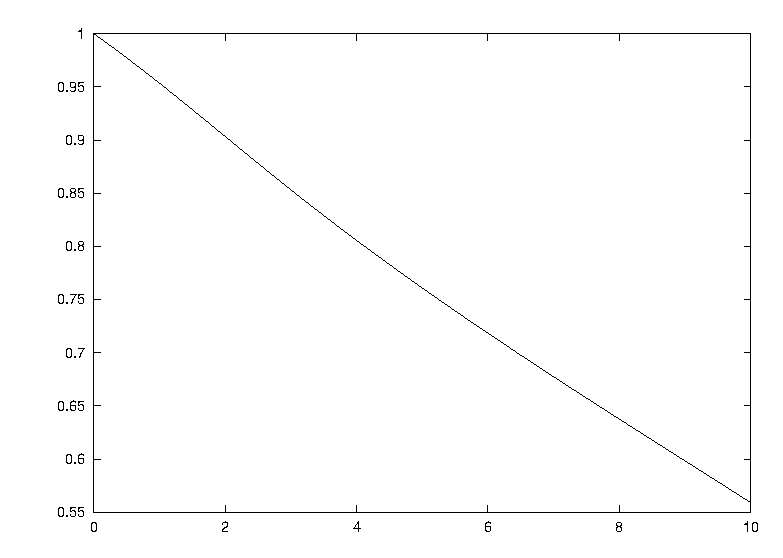
\includegraphics[scale=0.75]{df.eps}
  \caption{Křivka diskotních faktorů vypočtených na základě hodnot vektoru $\hat{\beta}$ dle modelu (4.6)}
  \label{df}
\end{figure}
\begin{figure}
  \centering
  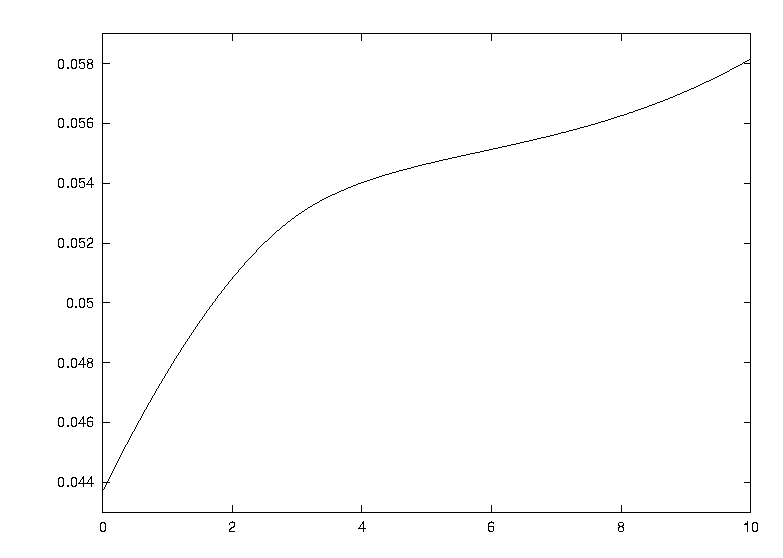
\includegraphics[scale=0.75]{zero.eps}
  \caption{Křivka zero sazeb, které odpovídají křivce diskontních sazeb uvedené na obrázku (\ref{df})}
  \label{zero}
\end{figure}
Obrázky (\ref{df}) a (\ref{zero}) zachycují křivku diskontních faktorů a křivku zero sazeb odpovídajících vypočteným parametrům. $\clubsuit$

\subsubsection{Konstrukce zero křivky}

Alternativou k diskontní křivce je přímé odvození křivky zero sazeb, ze které jsou následně odvozeny diskontní faktory nezbytné pro výpočet modelové ceny dluhopisu. Tento přístup má narozdíl od výše popisovaných metod výhodu v tom, že parametry modelu mají ekonomickou interpretaci. Nosnou myšlenkou je aproximace zero křivky funkcí $G(0,s;u)$, kde $u$ je sloupcový vektor parametrů, které je nutné odhadnout. Odhad vektoru $u$ je řešením nelineárního problému
\begin{equation*}
\underset{u}{\min} \sum_{j=1}^n \Bigg( \frac{P_0^j - \hat{P_0^j}}{\omega_j}\Bigg)^2 = \underset{u}{\min} J(u)
\end{equation*}
kde $\omega_j$ představuje váhu $j$-tého dluhopisu opět definovanou jako
\begin{equation*}
\omega_j = \frac{d P_0^j}{dy_j(0)}
\end{equation*}
a $\hat{P_0^j}$ je modelovou cenou dluhopisu
\begin{equation*}
\hat{P_0^j} = \sum_{\substack{s=T_j-\alpha_j+1 \\ s > 0}} F_s^j e^{-sG(0,s;\beta)}
\end{equation*}
Výše uvedený optimalizační problém je třeba řešit pomocí Newtonovy metody (viz. příloha B této kapitoly). Pro funkci $G(0,s;\beta)$ lze použít některý z níže uvedených modelů.\\

\noindent \textbf{Nelson-Siegel model~} Nelson a Siegel (1987) odvodili rovnici, která je řešením diferenciální rovnice popisující dynamiku úrokových sazeb. Tato rovnice má tvar
\begin{equation*}
f(0, \theta) = \beta_0 + \beta_1 e^{-\frac{\theta}{\tau_1}} + \beta_2 \frac{\theta}{\tau_1}e^{-\frac{\theta}{\tau_1}}
\end{equation*}
kde $f(0, \theta)$ je okamžitou forwardovou sazbou platnou v čase $\theta$. Parametr $\tau_1$ je nutné vhodně zvolit a parametry $\beta_0$, $\beta_1$, $\beta_2$ představují prvky vektoru $u$, který je třeba odhadnout. S využitím rovnice pro výpočet spojité zero sazby se splatností v čase $\theta$ 
\begin{equation*}
R^c(0,\theta) = \frac{1}{\theta} \int_0^{\theta} f(0,s)ds
\end{equation*}
lze odvodit
\begin{equation*}
R^c(0, \theta) = \beta_0 + \beta_1 \Bigg( \frac{1 - e^{-\frac{\theta}{\tau_1}}}{\frac{\theta}{\tau_1}}\Bigg) + \beta_2 \Bigg( \frac{1 - e^{-\frac{\theta}{\tau_1}}}{\frac{\theta}{\tau_1}} - e^{-\frac{\theta}{\tau_1}} \Bigg)
\end{equation*}
Parametr $\beta_0$ představuje limitu $R^c(0, \theta)$ pro $\theta$ blížící se nekonečnu. Na tento parametr je tedy možné nahlížet jako na dlouhodobou úrokovou míru. Parametr $\beta_1$ představuje limitu $R^c(0, \theta)$ pro $\theta$ blížící se nule, a proto je možné ho interpretovat jako spread mezi dlouhodobou a krátkodobou úrokovou mírou. Parametr $\beta_2$ je parametrem zakřivení zero křivky. A konečně parametr $\tau_1$ představuje míru, s jakou se z modelu "vytrácí" krátkodobé a střednědobé komponenty. Parametry $\beta_0$, $\beta_1$ popř. $\beta_2$ tedy mohou být spojovány s paralelním posunem, změnou sklonu popř. zakřivení zero křivky, jak vyplývá ze senzitivity
\begin{equation*}
S_i = \frac{\partial R^c(0, \theta)}{\partial \beta_i}
\end{equation*}
Senzitivita $S_0$ je konstatní pro všechny maturity. Senzitivita $S_1$ reprezentující sklon křivky je největší pro krátké maturity a s rostoucí splatností klesá k nule. Senzitivita $S_2$ je typicky nulová pro krátký konec křivky, dosahuje maxima ve střední části křivky a na dlouhém konci křivky opět klesá k nule.

Pomocí Nelson-Siegel modelu jsme schopni simulovat rostoucí, klesající popř. plochou křivku. Nejsme však schopni získat profil zlomové křivky. Aby odstranil tento nedostatek, modifikoval Svensson (1994) model do podoby
\begin{equation*}
R^c(0, \theta) = \beta_0 + \beta_1 \Bigg( \frac{1 - e^{-\frac{\theta}{\tau_1}}}{\frac{\theta}{\tau_1}} \Bigg) + \beta_2 \Bigg( \frac{1 - e^{-\frac{\theta}{\theta_1}}}{\frac{\theta}{\tau_1}} - e^{-\frac{\theta}{\tau_1}}\Bigg) + \beta_3 \Bigg( \frac{1 - e^{-\frac{\theta}{\tau_2}}}{\frac{\theta}{\tau_2}} - e^{-\frac{\theta}{\tau_2}}\Bigg)
\end{equation*}
Výše uvedená rovnice je někdy nazývána rozšířeným Nelson-Siegel modelem.\\

\noindent \textbf{Rozšířený Vašíčkův model~} Tento model je inspirován řešením původního Vašíčkova modelu (1977), ve kterém krátkodobé úrokové míry $r_t$ sledovaly Ornstein-Uhlenbeck difúzní proces
\begin{equation*}
dr_t = a(b-r_t)dt + \sigma dW_t
\end{equation*}
V tomto modelu je zero sazba dána funkcí
\begin{equation*}
R^c(0,\theta) = R_{\infty} - (R_{\infty} - r_0)\frac{1 - e^{-a \theta}}{a \theta} + \frac{\sigma^2}{a^2}\frac{\Big(1 - e^{-a \theta}\Big)^2}{4a \theta}
\end{equation*}
kde
\begin{equation*}
R_{\infty} = b + \frac{\lambda \sigma}{a} - \frac{\sigma^2}{2a^2}
\end{equation*}
a $\lambda$ představuje konstantní rizikovou prémii.

Tento model byl rozšířen do podoby
\begin{equation*}
R^c(0,\theta) = G(0, \theta; u)
\end{equation*}
kde
\begin{equation*}
u = (L_0, S_0, \gamma_0, a)^T
\end{equation*}
Funkce $G$, která je také nazývána Rozšířený Vašíčkův model 1, má tvar
\begin{equation*}
G(0,\theta; u) = L_0 - S_0 \frac{1 - e^{-a\theta}}{a \theta} + \gamma_0 \frac{(1 - e^{-a \theta})^2}{4a \theta}
\end{equation*}
Interpretace parametrů tohoto modelu je následující. $L_0$ je limita $R^c(0,\theta)$ pro $\theta$ blížící se nekonečnu. $L_0$ lze tedy považovat za dlouhodobou úrokovou míru. Parametr $S_0$ je limitou pro $L_0 - R^c(0, \theta)$, kde $\theta$ se blíží nule, a proto je možné na něj nahlížet jako na spread mezi dlouhodobou a krátkodobou úrokovou mírou. Parametr $\gamma_0$ představuje zakřivení vztažené k volatilitě krátkodobé úrokové sazby $\sigma$. Parametr $a$ představuje míru, se kterou v čase konverguje krátkodobá úroková sazba k dlouhodobé průměrné úrokové sazbě.

Další rozšíření modelu označované jako Rozšířený Vašíčkův model 2 má podobu
\begin{equation*}
G(0, \theta; U) = L_0 - S_0 \frac{1 - e^{-a \theta}}{a \theta} + \gamma_0 \frac{(1 - e^{-a \theta})^2}{4a\theta} - T_0 \frac{1 - e^{-b \theta}}{b \theta} + K_0 \frac{(1 - e^{-b \theta})^2}{4b \theta}
\end{equation*}

\section{Odvození mezibankovní zero křivky}

Mezibankovní zero křivka se skládá ze tří základních druhů instrumentů
\begin{itemize}
\item depozitních sazeb
\item FRA a futures
\item swapových sazeb
\end{itemize}
Depozitní sazby se zpravidla používají pro odvození zero sazeb se platností do tří měsíců. Zero sazby se splatností tři měsíce až jeden rok bývají vypočteny z FRA a futures. Zero sazby se splatností nad jeden rok jsou obvykle odvozeny ze swapových sazeb.

\subsection{Depozitní sazby}

Depozitní sazba představuje úrokovou sazbu, za kterou je možné na mezibankovním trhu získat popř. uložit finanční prostředky. Splatnost obchodu nepřekračuje jeden rok. Z depozitních sazeb lze jednoduše dopočítat zero sazby dle rovnice
\begin{equation*}
R(0, \theta) = \Bigg(1 + I(0,\theta)\frac{\Delta t}{B_{depo}} \Bigg)^{\frac{B_{zero}}{\Delta t}} - 1
\end{equation*}
kde $I(0,\theta)$ je depozitní sazba platná pro časové období od součastnosti do $\theta$, $\Delta t$ představuje počet kalendářních dní v tomto období a $B_{depo}$ popř. $B_{zero}$ jsou roční báze pro depozitní popř. zero sazby. Standardně platí $B_{depo} = 360$ a $B_{zero} = 365$.

\subsection{FRA a futures}

FRA a futures jsou zpravidla použity při konstrukci středního segmentu mezibankovní zero křivky. Tyto sazby se mohou z hlediska splatnosti částečně překrývat s depozitními sazbami. V praxi jsou preferovány právě FRA a futures, protože jsou v porovnání s mezibankovními sazbami likvidnější a lépe odráží skutečnou situaci na trhu.

\subsubsection{Forward rate agreement}

Podstatou FRA je fixace budoucí úrokové sazby. Např. v rámci 3x6 FRA je fixována úroková sazba pro období 3 až 6 měsíců od okamžiku sjednání obchodu. Protože po uplynutí 3 měsíců je známa částka, která bude vyplacena v době splatnosti obchodu, je možné FRA vypořádat k datu fixace úrokové sazby. To je také běžnou praxí a jedná se o specifikum FRA obchodů.

\subsection{Futures}

Pro konstrukci mezibankovní zero křivky lze použít tříměsíční futures na depozitní sazby. Cena této futures splatné v čase $\theta$ je rovna
\begin{equation*}
F_{3M,\theta} = 100 - I(\theta - 3M, \theta)
\end{equation*}
kde $I(\theta - 3M, \theta)$ je podkladová tříměsíční forwardová úroková sazba pro období $\theta - 3M$ až $\theta$. Dle této rovnice je možné z cen futures, které jsou kotovány na trhu, dopočíst forwardovou úrokovou sazbu.

\subsubsection{Výpočet zero sazby}

Z výše uvedeného je zřejmé, že FRA má charakter forwardové úrokové sazby a futures lze snadno převést na ekvivalentní forwardovou úrokovou sazbu.

Uvažujme depozitní sazbu $I(0, \theta_0)$ a forwardovou sazbu $I(\theta_0, \theta_1)$. Zero sazba $R(0, \theta_1)$ je rovna
\begin{equation*}
R(0,\theta_1) = \Bigg[ \Big( 1 + \frac{\Delta t_0}{B_{depo}}I(0,\theta_0)\Big) \Big( 1 + \frac{\Delta t_1}{B_{depo}} I(\theta_0, \theta_1) \Big)\Bigg]^{\frac{B_{zero}}{\Delta t_0 + \Delta t_1}} - 1
\end{equation*}
kde $\Delta t_0$ je počet kalendářních dní v časové periodě od součastnosti do $\theta_0$ a $\Delta t_1$ je počet kalendářních dní v časové periodě od $\theta_0$ do $\theta_1$.

\subsection{Swapové sazby}

Uvažujme úrokový swap se splatností $\theta$ roků. Nechť má floatová noha šestiměsíční a fixní noha roční frekvenci výplaty. Jestliže budeme v době splatnosti úrokového swapu uvažovat imaginární směnu nominálů, je současná hodnota floatové nohy v době uzavření úrokového swapu rovna jedné. Aby byla hodnota úrokového swapu v okamžiku jeho uzavření nulová, musí platit
\begin{equation*}
\sum_{i = 1}^{\theta} \frac{S(0,\theta)}{(1 + R(0,i))^i} + \frac{1}{(1 + R(0,\theta))^{\theta}} = 1
\end{equation*} 
kde $S(0,\theta)$ je swapová úroková sazba pro úrokový swap se splatností $\theta$ roků. Platí $S(0,1) = I(0,1)$, kde $I(0,1)$ je rovna jednoroční depozitní sazbě popř. jednoroční sazbě odvozené z FRA resp. futures kotací.

Abychom mohli z výše uvedené rovnice vyjádřit $R(0,\theta)$, musíme znát všechna $R(0, i)$ pro $i < \theta$. Zero sazby je tak třeba vypočíst postupně.

\subsection{Lineární, kubická a log-lineární interpolace}

Po získání izolovaných zero sazeb je třeba pomocí interpolace odvodit zero křivku mezi těmito sazbami. Je možné použít lineární, kubickou popř. log-lineární interpolaci.

Lineární a kubická interpolace byly vysvětleny v předchozí kapitole. Definice log-lineární interpolace je následující. Uvažujme diskontní faktory $B(0,x)$ a $B(0,z)$ a pokusme se vypočíst diskontní faktor $B(0,y)$ pro $x < y < z$. Aplikací log-lineární interpolace získáme
\begin{equation*}
\ln B(0,y) = \frac{z-y}{z-x} \ln B(0,x) + \frac{y - x}{z - x} \ln B(0,z)
\end{equation*}
Vzhledem k tomu, že diskontní faktor lze s použitím spojité zero sazby $R^c(0,\theta)$ vypočíst dle
\begin{equation*}
B(0,\theta) = e^{-\theta R^c(0,\theta)}
\end{equation*}
přechází výše uvedená rovnice do tvaru
\begin{equation*}
R^c(0,y)y = \frac{z - y}{z - x}R^c(0,x)x + \frac{y - x}{z - x}R^c(0,z)z
\end{equation*}

\subsection{Metoda nejmenších čtverců založená na sazbách}

Aplikace metody nejmenších čtverců je v případě odvození mezibankovní zero křivky totožná s aplikací této metody při odvození diskontní křivky. Předpokládejme, že jsme na základě tržních data vypočetly $N$ zero sazeb. Pro teoretickou zero křivku použijme model založený na B-segmentové funkci.
\begin{equation*}
\hat{R}(0, \theta) = \sum_l c_l B_l^3(\theta) = \sum_l c_l \Bigg( \sum_{j=l}^{l+4} \Big[ \prod_{\substack{i=l \\ i \neq j}} \frac{1}{\lambda_i - \lambda_j}\Big](\theta - \lambda_j)_{+}^3 \Bigg)
\end{equation*}
Skládá-li se teoretická zero křivka z $x$ segmentů, tj. je-li řád její báze roven $x+3$, musí parametry $\lambda_i$ splňovat podmínku
\begin{equation}
\lambda_{-3} < \lambda_{-2} < \lambda_{-1} < \lambda_0 = 0 < \dots < \lambda_x = t_{x-1} < \lambda_{x+1} < \lambda_{x+2} < \lambda_{x+3}
\end{equation}
kde intervaly $(0, t_0)$, $(t_0 - t_1)$, ..., $(t_{x-2}, t_{x-1})$ definují jednotlivé segmenty.

V dalším kroce je třeba pomocí metody nejmenších čtverců provést odhad parametrů $c_l$.
\begin{equation*}
\underset{c_l}{\min} \sum_{n=1}^{N}\Big(R(0,n) - \hat{R}(0,n) \Big)^2
\end{equation*}

\subsection{Metoda nejmenších čtverců založená na cenách dluhopisů}

V rámci této metody jsou nejprve tržní data přepočtena na zero sazby, ze kterých jsou následně vypočteny diskontní faktory. Tyto diskontní faktory lze chápat jako cenu diskontních dluhopisů. Předpokládejme, že máme k dispozici $N$ takovýchto cen. Označme tyto ceny jako $P_i$, kde $i = 1,2, \dots, N$.

V dalším kroku zkonstruujme model teoretické diskontní křivky pomocí B-segmentové funkce.
\begin{equation*}
B(0, \theta) = \sum_l c_l B_l^3(\theta) = \sum_l c_l \Bigg( \sum_{j = l}^{l+4}\Big[ \prod_{\substack{i=l \\ i \neq j}}\frac{1}{\lambda_i - \lambda_j}\Big](\theta - \lambda_j)_{+}^3 \Bigg)
\end{equation*}
Parametry $\lambda_i$ musí opět splňovat podmínku (4.15).

V posledním kroku je třeba odhadnout parametry $c_l$ pomocí metody nejmenších čtverců. Označme teoretickou cenu diskontního dluhopisu, která je založena na modelované diskontní křivce a která odpovídá ceně $P_i$ odvozené z třžních dat, jako $\hat{P}_i$. Optimalizační problém má tak podobu 
\begin{equation*}
\underset{c_l}{\min}\sum_{n=1}^N \Big(P_i - \hat{P}_i \Big)^2
\end{equation*}

\section{Výpočet kreditního spreadu}

Kreditní spread vyjadřuje míru kreditního rizika dluhopisu relativně ke zvolenému benchmarku. Na základě kreditních spreadů vypočtených z dluhopisů, které lze s ohledem na kreditní riziko považovat za homogenní skupinu, lze zkonstruovat tzv. křivku kreditních spreadů. Dluhopisy zpravidla považujeme za homogenní, pokud jsou
\begin{itemize}
\item denominovány ve stejné měně
\item emitovány subjekty se shodným ratingem
\item emitovány subjekty podnikajícími ve shodném sektoru
\end{itemize}
Kreditní spread pro skupinu homogenních dluhopisů může být odvozen přímou nebo nepřímou metodou.

\subsection{Nepřímá metoda}

V případě nepřímé metody je nejprve vypočtena zero křivka, která slouží jako srovnávací základna. Tuto funkci zpravidla plní mezibankovní zero křivka popř. zero křivka zkonstruovaná ze státních dluhopisů. Dále je na základě zkoumaných dluhopisů zkonstruována zero křivka. Křivka kreditních spreadů je dána rozdílem těchto dvou zero křivek.

Nevýhodou tohoto přístupu je závislost kreditních spreadů na zvoleném modelu pro výpočet zero křivek a počtu segmentů. Další nevýhodou je skutečnost, že takto zkonstruovaná křivka kreditních spreadů nemusí být hladká ani monotónní.

\subsection{Přímá metoda}

Předpokládejme, že chceme zkonstruovat křivku kreditních spreadů pro $n$ rizikových skupin dluhopisů. V dalším textu budeme používat následující značení.
\begin{center}
\begin{tabular}{l l}
$J_i$ & počet dluhopisů v $i$-té rizikové skupině, kde $i = 1,2, \dots, n$;\\
 & $J_0$ je počet dluhopisů, které tvoří srovnávací základnu\\
$P_t^{j_i}$ & tržní cena $j$-tého dluhopisu v $i$-té rizikové skupině v čase $t$\\
$\hat{P}_t^{j_i}$ & teoretická cena $j$-tého dluhopisu v $i$-té rizikové skupině v čase $t$\\
$P_t^i$ & vektor tržních cen dluhopisů v $i$-té rizikové skupině\\
$\hat{P}_t^i$ & vektor teoretických cen dluhopisů v $i$-té rizikové skupině\\
$T_{j_i}$ & splatnost $j$-tého dluhopisu $i$-té rizikové skupiny v letech\\
$F_s^{j_i}$ & cash-flow generované $j$-tým dluhopisem z $i$-té rizikové skupiny v čase $t$\\
$\alpha_{j_i}$ & počet cash-flow generovaných $j$-tým dluhopisem $i$-té rizikové skupiny\\
$B_i(t,s)$ & diskontní faktor $i$-té skupiny; alternativně lze chápat jako cenu diskontního\\
 & dluhopisu z $i$-té rizikové skupiny se splatností v $s$ k časovému okamžiku $t$
\end{tabular}
\end{center}

\subsubsection{Aditivní kreditní spread}

Diskontní faktor spojený s $i$-tou rizikovou skupinou je vyjádřen jako součet diskontního faktoru srovnávací rizikové třídy a funkce kreditního spreadu. Teoretická cena dluhopisu dána rovnicí
\begin{equation*}
\hat{P}_t^{j_i} = \sum_{\substack{s = T_{j_i} - \alpha_{j_i} + 1 \\ s > 0}}F_s^{j_i} \Big( B_0(t,s) + S_i(t,s)\Big)
\end{equation*}
Houweling a kol. (1999) navrhují modelovat diskontní funkce pomocí B-segmentových funkcí. Jestliže budeme stejně jako v předchozích případech uvažovat třísegmentovou funkci, mají příslušné rovnice tvar
\begin{equation*}
B_0(0,s) = B_0(s) = \sum_{k=-3}^2 c_{0,k}\Bigg( \sum_{m=k}^{k+4}\Bigg[ \prod_{\substack{l = k \\ l \neq m}} \frac{1}{\lambda_l - \lambda_m}\Bigg](s - \lambda_m)_{+}^3 \Bigg)
\end{equation*}
\begin{equation*}
S_i(0,s) = S_i(s) = \sum_{k=-3}^2 c_{i,k}\Bigg( \sum_{m=k}^{k+4}\Bigg[ \prod_{\substack{l = k \\ l \neq m}} \frac{1}{\lambda_l - \lambda_m}\Bigg](s - \lambda_m)_{+}^3 \Bigg)
\end{equation*}
Výhodou aditivního kreditního spreadu je zachování linearity problému. To umožňuje odhad parametrů pomocí metody nejmenších čtverců. Vedle B-segmentové funkce je možné použít také polynomickou popř. exponenciální segmentovou funkce.

\subsubsection{Multiplikativní kreditní spread}

V případě multiplikativního kreditního spreadu lze teoretickou cenu dluhopisu vyjádřit jako
\begin{equation*}
\hat{P}_t^{j_i} = \sum_{\substack{s = T_{j_i} - \alpha_{j_i} + 1 \\ s > 0}}F_s^{j_i} \Big( B_0(t,s) T_i(t,s)\Big)
\end{equation*}
Pro zero zero sazbu pak platí
\begin{equation*}
e^{-(s-t)R_i^c(t,s-t)} = e^{-(s-t)R^c(t,s-t)}e^{-(s-t)t_i^c(t,s-t)}
\end{equation*}
\begin{equation*}
R_i^c(t,s-t) = R^c(t,s-t)+t_i^c(t,s-t)
\end{equation*}
Srovnávací zero křivku je možné modelovat pomocí B-segmentové funkce. Almeida a kol. (1998, 2000) navrhovali pro modelování kreditního spreadu použít Legendrovy polynomy. Tvar rovnic je tak následující 
\begin{equation*}
R(0,s) = \sum_{k=-3}^2 c_{0,k}\Bigg( \sum_{m=k}^{k+4}\Bigg[ \prod_{\substack{l = k \\ l \neq m}} \frac{1}{\lambda_l - \lambda_m}\Bigg](s - \lambda_m)_{+}^3 \Bigg)
\end{equation*}
\begin{equation*}
t_i(0,s) = \sum_{p \ge 0} c_{i,p} P_p \Big( \frac{2s}{M} - 1 \Big)
\end{equation*}
kde Legenderův polynom $P_p(x)$ je definován jako
\begin{equation*}
P_p(x) = \frac{1}{2^p p!}\frac{\partial p}{\partial x^n}(x^2 - 1)^p~~~\forall p = 0,1,2,...
\end{equation*}
Protože se jedná o nelineární problém není možné pro odhad parametrů použít metodu nejmenších čtverců - je nutné použít Newtonovu metodu.

\section{Příloha A: Metoda nejmejších čtverců}

Uvažujme náhodný vektor
\begin{equation*}
Y =
\begin{bmatrix}
Y_1 \\
Y_2 \\
\vdots \\
Y_n
\end{bmatrix}
\end{equation*}
a matici daných čísel $X_{n \times k}$. Předpokládejme, že se $Y$ řídí tzv. lineárním modelem
\begin{equation*}
Y = \beta X + \varepsilon
\end{equation*}
kde $\beta$ je vektor neznámých parametrů a $\varepsilon$ je vektor náhodných veličin splňujících podmínky
\begin{gather*}
E[\varepsilon] = 0 \\
D[\varepsilon] = \sigma^2 I
\end{gather*}
Parametr $\sigma^2 > 0$ rovněž není znám. Lze však pozorovat vektor $Y$. Vektor $\varepsilon$ je možné charakterizovat jako vektor chyb. Těmito chybami se zpravidla rozumnějí chyby vyplývající z nepřesností při stanovování vektoru $Y$, někdy se pod takové chyby zahrnují i odchylky od přesné lineární závislosti $Y = \beta X$. Vektor $\varepsilon$ se pozorovat nedá. Předpoklad $E[\varepsilon] = 0$ odpovídá tomu, že pozorování vektoru $Y$ nejsou zatížena systematickými chybami. Vztah $D[\varepsilon] = \sigma^2 I$ zase říká, že měření jednotlivých složek vektoru $Y$ jsou prováděna se stejnou přesností a že chyby měření různých složek vektoru $Y$ jsou nekorelované.

Pro zjednodušení výkladu budeme v tomto odstavci předpokládat, že hodnost matice $X$ je rovna $k$ a že $n > k$. Lineární model splňující tyto dodatečné podmínky se nazývá regresní.

Z dosavadních předpokladů plyne, že $E[Y] = \beta X$ a $D[Y] = \sigma^2 I$. Vektor $\beta$ se odhaduje metodou nejmenších čtverců, tj. z podmínky, že výraz
\begin{equation*}
S(\beta) = (Y - \beta X)^T(Y - \beta X)
\end{equation*}
má být minimální. Tento odhad označme $\hat{\beta}$.

Z teorie matic je známo, že pro jakoukoli matici $A$ platí $h(A) = h(AA^T) = h(A^TA)$, kde $h(A)$ značí hodnot matice $A$. Jelikož $h(X) = k$ a matice $X^TX$ je typu $k \times k$, plyne odtud, že matice $X^TX$ je regulární a tím pádem existuje inverzní matice $(X^TX)^{-1}$.

Pro odhad $\hat{\beta}$ platí
\begin{equation*}
\hat{\beta} = (X^TX)^{-1}X^TY
\end{equation*}

\noindent \textbf{Důkaz:} Nejprve se snadno dosazením ověří, že vektor $\hat{\beta}$ ve výše uvedeném tvrzení splňuje podmínku $X^T(Y - \hat{\beta}X) = 0$. Pak napíšeme $S(\beta)$ ve tvaru
\begin{equation*}
S(\beta) = [(Y - \hat{\beta}X) + (\hat{\beta}X - \beta X)]^T[(Y - \hat{\beta}X) + (\hat{\beta}X - \beta X)]
\end{equation*}
Po roznásobení a po použití podmínky $X^T(Y - \hat{\beta}X) = 0$ získáme
\begin{equation*}
S(\beta) = (Y - \hat{\beta}X)^T(Y - \hat{\beta}X) + (\hat{\beta} - \beta)^T X^T X (\hat{\beta} - \beta)
\end{equation*}
Z předpokladu $h(X) = k$ vyplývá, že matice $X^T X$ je pozitivně definitní. Proto
\begin{equation*}
(\hat{\beta} - \beta)^T X^T X (\hat{\beta} - \beta) \ge 0
\end{equation*}
a rovnost nastává práve pro $\beta = \hat{\beta}$. $\spadesuit$

\section{Příloha B: Newtonův algoritmus}

Uvažujme výchozí bod
\begin{equation*}
u_0 =
\begin{bmatrix}
a_0 \\
a_1 \\
\vdots \\
a_n \\
\end{bmatrix}
\end{equation*}
Dále uvažujme funkci $J(u)$ a Taylorův rozvoj této funkce (resp. jeho kvadratickou aproximaci) kolem bodu $u_0$
\begin{equation}
J(u) \approx J(u_0) + \bigtriangledown J(u_0) + \frac{1}{2}(u - u_0)^T \bigtriangledown^2 J(u_0)(u - u_0)
\end{equation}
kde
\begin{equation*}
\bigtriangledown J(u_0) =
\begin{bmatrix}
\frac{\partial J}{\partial a_0}u_0 \\
\frac{\partial J}{\partial a_1}u_0 \\
\vdots \\
\frac{\partial J}{\partial a_n}u_0
\end{bmatrix}
\end{equation*}
a
\begin{equation*}
\bigtriangledown^2 J(u_0) =
\begin{bmatrix}
\frac{\partial^2 J}{\partial a_0^2}u_0 & \frac{\partial^2 J}{\partial a_0 \partial a_1}u_0 & \dots & \frac{\partial^2 J}{\partial a_0 \partial a_n}u_0 \\
\frac{\partial^2 J}{\partial a_0 \partial a_1}u_0 & \frac{\partial^2 J}{\partial a_1^2}u_0 & \dots & \frac{\partial^2 J}{\partial a_1 \partial a_n}u_0 \\
\vdots & \vdots & \ddots & \vdots \\
\frac{\partial^2 J}{\partial a_0 \partial a_n}u_0 & \frac{\partial^2 J}{\partial a_1 \partial a_n}u_0 & \dots & \frac{\partial^2 J}{\partial a_n^2}u_0 \\
\end{bmatrix}
\end{equation*}
Předpokládejme, že hledáme minimum funkce $J(u)$, kterému odpovídá bod $u_1$. V tomto bodě musí funkce $J$ splňovat podmínku
\begin{equation*}
\frac{J(u_1)}{\partial u_1} = 0
\end{equation*}
což lze derivací (4.16) vyjádřit také jako
\begin{equation}
[1~~1~~1] \bigtriangledown J(u_0) + [1~~1~~1] \bigtriangledown^2 J(u_0)(u_1 - u_0) = 0
\end{equation}
Hledaný bod $u_1$ lze vypočíst dle
\begin{equation*}
u_1 = u_0 - (\bigtriangledown^2 J(u_0))^{-1} \bigtriangledown J(u_0) 
\end{equation*}
Vzhledem k tomu, že pro nalezení bodu minima byla použita aproximace, je třeba tento postup několikrát zopakovat, dokud nezískáme výsledek s požadovanou přesností.
\begin{equation}
u_{k+1} = u_k - (\bigtriangledown^2 J(u_k))^{-1} \bigtriangledown J(u_k) 
\end{equation}
Je třeba si uvědomit, že (4.17) je podmínkou pro nalezení extrému funkce nikoliv jejího minima. Pokud nebude počáteční odhad $u_0$ dostatečně blízko minimu funkce, nemusí tento postup vést k požadovanému výsledku. Součástí procedury by tak měla být konktrola, že je splněna podmínka $J(u_{k+1}) < J(u_k)$.\\

\noindent \textbf{Příklad:} Nalezněme minimum funkce $e^{(e+2)^2}$. První resp. druhá derivace této funkce dle $x$ jsou
\begin{equation*}
\frac{\partial f(x)}{\partial x} = 2(x+2)e^{(x+2)^2}
\end{equation*}
\begin{equation*}
\frac{\partial^2 f(x)}{\partial x^2} = 2(2x+5)e^{(x+2)^2}
\end{equation*}
Rovnice (4.18) má tedy podobu
\begin{equation}
u_{k+1} = u_k - \frac{x+2}{2x+5}
\end{equation}
Výpočet minima funkce zahájíme počátečním dohadem $x_0 = -1$. Postupným dosazováním do rovnice (4.15) získáváme
\begin{gather*}
u_1 = -1.33333 \\
u_2 = -1.61905 \\
u_3 = -1.83526 \\
u_4 = -1.95917 \\
u_5 = -1.99998 \\
\end{gather*}
Minimum námi uvažované funkce je v bodě $u = 2$. Po páté iteraci se tedy dostáváme dostatečně blízko k přesnému řešení. $\clubsuit$
\part{Zajištění úrokového rizika}

\chapter{Durace}

\section{Základy úrokového rizika}

\subsection{Splatnost a kupónová sazba}

Cena dluhopisů je negativně závislá na pohybu úrokových sazeb. Jestliže úrokové sazby rostou, ceny dluhopisů klesají na naopak. Pokles úrokových sazeb vede k vyššímu procentuálnímu růstu ceny než je procentuální snížení ceny z titulu ekvivalentního nárůstu úrokových sazeb.

Míra citlivosti ceny dluhopisu na změnu úrokových sazeb roste s jeho splatností. Ceny dlouhodobých dluhopisů jsou proto volatilnější než ceny krátkodobých dluhopisů. Tato citlivost roste klesajícím tempem s narůstající dobou do splatnosti dluhopisu.

Míra citlivosti ceny dluhopisu na změnu úrokových sazeb je funkcí kupónové sazby. Mezi oběma parametry je nepřímá úměra. Dluhopisy s vyšším kupónovou sazbou jsou méně citlivé na změnu úrokových sazeb než dluhopisy s nízkou úrokovou sazbou.

\subsection{Reinvestiční riziko}

Vraťme se k pojmu "výnosová míra do splatnosti" (YTM), který jsme představili v druhé kapitole. Je důležité si uvědomit, že YTM dluhopisu je výnos, který získá investor pouze za předpokladu, že uvažovaný dluhopis bude držet do splatnosti a veškeré vyplacené kupóny bude reinvestovat za úrokovou sazbu rovnající se YTM. V praxi je však běžné, výnosová míra z reinvestovaných kupónů je odlišná od YTM, což je podstata tzv. reinvestičního rizika.

Je zřejmé, že reinvestiční riziko je funkcí kupónové sazby a zbytkové splatnosti dluhopisu. Mezi reinvestičním rizikem a kupónovou sazbou popř. zbytkovou splatností je přímá úměra. Reinvestiční riziko se tedy nejvýrazněji projevuje v případě dluhodobých dluhopisů s vysokou kupónovou sazbou.

\subsection{Kapitálové riziko}

Jak již bylo řečeno, růst úrokových sazeb má za následek pokles ceny dluhopisu a naopak. Protože YTM má z pohledu dluhopisu charakter průměrné úrokové sazby, platí tento vztah také mezi cenou dluhopisu a YTM.

Reinvestiční riziko a kapitálové riziko se vzájemně kompenzují. Růst YTM má za následkem pokles ceny dluhopisů, na druhé straně však zvyšuje výnos z reinvestovaných kupónů.\\

\noindent \textbf{Příklad:} Uvažujme dvouletý dluhopis s nominální hodnotou 100 CZK, kupónovou sazbou 3.0\% a půlroční frekvencí vyplácení kupónů. Předpokládejme, že výchozí YTM je 4.5\%, čemuž odpovídá cena 97.161 CZK.
\begin{equation*}
\frac{3}{(1 + 0.0225)} + \frac{3}{(1 + 0.0225)^2} + \frac{3}{(1 + 0.0225)^3} + \frac{103}{(1 + 0.0225)^4} = 97.161
\end{equation*}
Jestliže dojde k poklesu YTM na 4.0\%, vzroste cena dluhopisu na 98.096 CZK.
\begin{equation*}
\frac{3}{(1 + 0.02)} + \frac{3}{(1 + 0.02)^2} + \frac{3}{(1 + 0.02)^3} + \frac{103}{(1 + 0.02)^4} = 98.096
\end{equation*}
Za šest měsíců se dluhopis zhodnotí na 100.058 CZK.
\begin{equation*}
98.096 \cdot (1 + 0.02) = 100.058
\end{equation*}
Zároveň však dojde k výplatě kupónu ve výši 1.5 CZK, v důsledku čehož klesne o stejnou částku, tj. na 98.558 CZK. Jestliže investujeme kupón na následujícího půl roku za YTM získáme dodatečný výnos 0.03 CZK.
\begin{equation*}
1.5 \cdot (1 + 0.02) = 1.530
\end{equation*}
Tímto způsobem lze postupovat až do splatnosti dluhopisu. Následující tabulky zachycují, jak se vyvíjí cena dluhopisu a výše reinvestovaného kupónu pro uvažovaný dluhopis v případě výnosové míry do splatnosti 4.0\% resp. 4.5\%. 
\begin{center}
\begin{tabular}{c c c c c}
\textbf{rok} & \textbf{YTM} & \textbf{cena}      & \textbf{reinvestovaný} & \textbf{celkem} \\
             &              & \textbf{dluhopisu} & \textbf{kupón}         &  \\
\hline
0.0 & 4.0 &  98.096 &       &         \\
0.5 & 4.0 &  98.558 & 1.500 & 100.058 \\
1.0 & 4.0 &  99.029 & 3.030 & 102.059 \\
1.5 & 4.0 &  99.510 & 4.591 & 104.100 \\
2.0 & 4.0 & 100.000 & 6.182 & 106.182 \\
\end{tabular}
\end{center}
\begin{center}
\begin{tabular}{c c c c c}
\textbf{rok} & \textbf{YTM} & \textbf{cena}      & \textbf{reinvestovaný} & \textbf{celkem} \\
             &              & \textbf{dluhopisu} & \textbf{kupón}         &  \\
\hline
0.0 & 4.5 &  97.161 &       & \\
0.5 & 4.5 &  97.848 & 1.500 &  99.348 \\
1.0 & 4.5 &  98.549 & 3.034 & 101.583 \\
1.5 & 4.5 &  99.267 & 4.602 & 103.869 \\
2.0 & 4.5 & 100.000 & 6.206 & 106.206
\end{tabular}
\end{center}
$\clubsuit$

\subsection{Kvantifikace úrokového rizika}

Uvažujme portfolio finančních instrumentů s fixním cash-flow. Předpokládejme, že tyto instrumenty generují v čase $t_i$ cash-flow $F_i$, kde $i = 1, 2, ..., m$. Hodnota portfolia $P$ může být vyjádřena jako suma diskontovaného cash-flow.
\begin{equation*}
P_t = \sum_{i = 1}^m F_i B(t,t_i) = \sum_{i = 1}^m \frac{F_i}{[1 + R(t, t_i - t)]^{t_i - t}}
\end{equation*}
Z výše uvedené rovnice je zřejmé, že hodnota portfolia $P_t$ je funkcí $m$ úrokových sazeb $R(t, t_i - t)$. V praxi je však relativně problematické zajistit se proti $m$ úrokovým veličinám, kde $m$ může být potenciálně vysoké číslo. Východiskem z tohoto problému je nahrazení uvažovaných $m$ úrokových sazeb jednou průměrnou úrokovou sazbou. Touto průměrnou úrokovou sazbou je YTM uvažovaného portfolia.

\section{Durace}

Logika durace je založena na myšlence nahrazení série úrokových sazeb, které ovlivňují hodnotu dluhopisu, jediným parametrem a to výnosovou mírou do splatnosti. Základem durace je první člen Taylorova rozvoje ceny portfolia podle YTM.

\subsection{Odvození durace pomocí Taylorova rozvoje}

Pomocí YTM lze hodnotu dluhopisu vyjádřit jako
\begin{equation}
P_t = P(y_t) = \sum_{i=1}^m \frac{F_i}{\Big(1+\frac{y_t}{n}\Big)^{\theta_i}}
\end{equation}
kde $n$ představuje frekvenci vyplácení kupónu, $y_t$ je YTM uvažovaného dluhopisu v čase $t$ vyjádřené ve frekvenci úročení odpovídající $n$, $F_i$ je cash-flow generované portfoliem v čase $t_i$ a $\theta_i$ představuje počet $\frac{1}{n}$ jednotek roku od $t$ do $t_i$\footnote{Je-li např. kupón vyplácen dvakrát do roka, představuje $\theta_i$ počet pololetí mezi časy $t$ a $t_i$.}. Protože YTM má ve vztahu k uvažovanému dluhopisu charakter průměrné úrokové sazby, je rovnice (5.1) značným zjednodušením reality. Toto zjednodušení je tím významnější, čím větší je sklon křivky časové struktura úrokových.

Druhým krokem je kvantifikace citlivosti ceny dluhopisu na změnu YTM. Tuto citlivost lze aproximovat pomocí prvního členu Taylorova rozvoje $P_t$ podle $y_t$.
\begin{equation}
d P(y) = P(y + dy) - P(y) = P'(y)dy + \mathcal{O}(y) \simeq D_\$(P(y))dy
\end{equation}
kde
\begin{equation*}
P'(y) = - \sum_{i=1}^m \frac{\frac{\theta_i}{n}F_i}{\Big( 1 + \frac{y}{n}\Big)^{\theta_i + 1}}
\end{equation*}
Derivací ceny dluhopisu podle YTM získáme tzv. dolarovou duraci $D_{\$}(P(y))$. Tato durace vyjadřuje, o kolik peněžních jednotek se změní cenu dluhopisu, pokud se YTM změní o $dy$.

Jestliže rovnici (5.2) vydělíme $P(y)$, získáme tzv. modifikovanou duraci.
\begin{equation}
\frac{dP(y)}{P(y)} = \frac{P'(y)}{P(y)}dy + \mathcal{O}(y) \simeq -D_m(P(y))dy
\end{equation}
Pomocí modifikované durace je možné vyjádřit procentní změnu ceny dluhopisu za předpokladu, že se YTM změní o $dy$.\\

\noindent \textbf{Příklad:} Uvažujme desetiletý dluhopis s kupónovou sazbou 6.0\%, roční frekvencí výplaty kupónu, výnosovou mírou do splatnosti 5.0\% a nominální hodnotou 100 USD. Cena tohoto dluhopisu je 107.72 USD. Dosazením do rovnice (5.2) resp. (5.3) získáme dolarovou duraci -809.67 USD resp. modifikovanou duraci 751.63\%. Jestliže se tedy YTM zvýší o 10 bazických bodů\footnote{Bazický pod je podjednotkou procentního bodu. Platí, že 100 bazických bodů je rovno jednomu procentnímu bodu.}, změní se hodnota dluhopisu přibližně o -0.80967 USD
\begin{equation*}
-809.67 \cdot 0.1\% = -0.80967
\end{equation*}
resp. přibližně o -0.75163\%.
\begin{equation*}
-7.5163 \cdot 0.1\% = -0.75163
\end{equation*}
$\clubsuit$

\subsection{Macauleyova durace}

V předchozí kapitole jsme si představili dolarovou a modifikovanou duraci. Dolarová durace představovala změnu hodnoty dluhopisu v absolutním, modifikovaná durace pak v relativním vyjádření. Běžně se však pojmem durace rozumí tzv. Macauleyova durace, která je definována jako
\begin{equation}
D(P(y)) = -(1 + y)\frac{P'(y)}{P(y)} = \frac{\sum_{i = 1}^m \frac{\theta_i F_i}{(1 + y)^{\theta_i}}}{P(y)}
\end{equation}
Macauleyovu duraci lze chápat jako váženou zbytkovou splatnost dluhopisu. Jednotlivé váhy mají podobu
\begin{equation*}
w_i = \frac{F_i}{P(y)(1+y)^{\theta_i}}
\end{equation*}
Z rovnice (5.4) je zřejmé, že Macauleyova durace je vždy menší než zbytková splatnost dluhopisu $\theta_m$. Vyjímkou jsou diskontní dluhopisy, kdy se Macauleyova durace rovná zbytkové splatnosti.

Předpokládejme, že se investiční horizont majitele dluhopisu shoduje s Macauleyovou durací uvažovaného dluhopisu. V tomto případě se investor nemusí obávat změny YTM - reinvestiční a kapitálové riziko se vzájemně vykompenzují.\\

\noindent \textbf{Příklad:} Uvažujme desetiletý dluhopis s kupónovou sazbou 6.0\%, roční frekvencí výplaty kupónu, výnosovou mírou do splatnosti 3.75\% a nominální hodnotou 100 USD. Cena tohoto dluhopisu je 118.48 USD a Macauleyova durace 8 roků.
\begin{center}
\begin{tabular}{c c c c c}
\textbf{rok} & \textbf{YTM} & \textbf{cena}      & \textbf{reinvestovaný} & \textbf{celkem} \\
             &              & \textbf{dluhopisu} & \textbf{kupón}         &  \\
\hline
0  & 3.75 & 118.479 &        &         \\
1  & 3.75 & 116.922 &  6.000 & 112.922 \\
2  & 3.75 & 115.306 & 12.225 & 127.531 \\
3  & 3.75 & 113.630 & 18.683 & 132.314 \\
4  & 3.75 & 111.891 & 25.384 & 137.275 \\
5  & 3.75 & 110.087 & 32.336 & 142.423 \\
6  & 3.75 & 108.216 & 39.549 & 147.764 \\
7  & 3.75 & 106.274 & 47.032 & 153.305 \\
8  & 3.75 & 104.259 & 54.795 & \underline{159.054}\\
9  & 3.75 & 102.169 & 62.850 & 165.019 \\
10 & 3.75 & 100.000 & 71.207 & 171.207
\end{tabular}
\end{center}
Jestliže se YTM změní z 3.75\% na 4.00\%, zůstane součet ceny dluhopisu a reinvestovaných kupónů na konci osmého roku téměr beze změny.
\begin{center}
\begin{tabular}{c c c c c}
\textbf{rok} & \textbf{YTM} & \textbf{cena}      & \textbf{reinvestovaný} & \textbf{celkem} \\
             &              & \textbf{dluhopisu} & \textbf{kupón}         &  \\
\hline
0  & 4.00 & 116.222 &       &          \\
1  & 4.00 & 114.871 &  6.000 & 120.871 \\
2  & 4.00 & 113.465 & 12.240 & 125.705 \\
3  & 4.00 & 112.004 & 18.730 & 130.734 \\
4  & 4.00 & 110.484 & 25.479 & 135.963 \\
5  & 4.00 & 108.904 & 32.498 & 141.402 \\
6  & 4.00 & 107.260 & 39.798 & 147.058 \\
7  & 4.00 & 105.550 & 47.390 & 152.940 \\
8  & 4.00 & 103.772 & 55.285 & \underline{159.058} \\
9  & 4.00 & 101.923 & 63.497 & 165.420 \\
10 & 4.00 & 100.000 & 72.037 & 172.037
\end{tabular}
\end{center}
$\clubsuit$\\

Macauleyova durace je aditivní. Uvažujeme portfolio $m$ dluhopisů, z nichž každý má duraci $D_i$ a váhu $w_i$, kde váha je vyjádřena jako podíl hodnoty dluhopisu na hodnotě portfolia. Durace portfolia je definována jako
\begin{equation*}
D_p = \sum_{i=1}^m w_i D_i
\end{equation*}

\subsection{Zajištění v praxi}

Uvažujme dluhopisy A a B. Dluhopis A má výnosovou míru do splatnosti $y$ a cenu $P(y)$, dluhopis B má výnosovu míru do splatnosti $y_1$ a cenu $H_1(y_1)$. Předpokládejme, že potřebujeme zajistit cenu dluhopisu A proti změně YTM a za tímto účelem jsme nakoupili $\phi$ kusů dluhopisu B. Cena výsledného portfolia je tak rovna
\begin{equation*}
P_p = P(y) + \phi H_1(y_1)
\end{equation*}
Cílem zajištění je vytvořit portfolio, jehož cena je imunní vůči malým změnám YTM. Předpokládejme, že křivka YTM je ovlivněna pouze parelelními posuny, což znamená $dy = dy_1$. Změnu ceny portfolia je tak možné vyjádřit jako
\begin{equation*}
dP_p = [P'(y) + \phi H_1'(y_1)]dy = 0
\end{equation*}
což lze přeformulovat do tvaru
\begin{equation*}
D_\$(P(y)) = - \phi (H_1(y_1))
\end{equation*}
resp. do tvaru
\begin{equation*}
P(y)D_m(P(y)) = - \phi H_1(y_1)(H_1(y_1))
\end{equation*}
Počet kusů dluhopisu B lze tak vyjádřit jako
\begin{equation*}
\phi = - \frac{D_\$(P(y))}{D_\$(H_1(y_1))} = - \frac{P(y)D_m(P(y))}{H_1(y_1)D_m(H_1(y_1))}
\end{equation*}

\chapter{Durace - pokračování}

Zajištění pomocí durace je velmi jednoduché. Tato metoda je však založena na několika poměrně značně restriktivních předpokladech.
\begin{itemize}
\item Prvním předpokladem je, že změnu ceny dluhopisu v závislosti na změně výnosu do splatnosti lze aproximovat prvním členem Taylorova rozvoje. Protože vztah mezi změnou ceny dluhopisu a YTM není lineární, platí tento předpoklad pouze pro velmi malé změny YTM.
\item Koncept durace je založen na YTM, což implikuje plochou výnosovou křivku. Plochá výnosová křivka znamená, že úrokové sazby jsou pouze paralelními posuny.
\end{itemize}

\section{Opuštění předpokladu infinityzimální změny YTM}

Koncepce durace je funkční pouze pro velmi malé změny úrokové sazby. To je důsledkem skutečnosti, že vztah mezi cenou dluhopisu a YTM není lineární. Durace dluhopisu se tak mění s každou změnou YTM. Tento problém lze částečně vyřešit aplikací druhého členu Taylorova rozvoje, tzv. konvexity. Změnu ceny dluhopisu tak lze vyjádřit jako
\begin{equation*}
dP(y) = P'(y)dy + \frac{1}{2}P''(y) (dy)^2 + \mathcal{O}((dy)^2) \simeq D_\$(P(y))dy + \frac{1}{2}C_\$(P(y))(dy)^2
\end{equation*}
kde
\begin{equation}
P''(y) = \sum_{i=1}^m \frac{\frac{\theta_i(\theta_i + 1)}{n^2}F_i}{\Big(1 + \frac{y}{n}\Big)^{\theta_i + 2}}
\end{equation}
Relativní změna ceny dluhopisu je pak dána rovnicí
\begin{equation*}
\frac{dP(y)}{P(y)} = -D_m P(y)dy + \frac{1}{2}C_m(P(y))(dy)^2
\end{equation*}
kde relativní konvexita $C_m$ je definována jako
\begin{equation*}
C_m(P(y)) = \frac{P''(y)}{P(y)}
\end{equation*}

\noindent \textbf{Příklad:} Uvažujme pětiletý dluhopis s kupónovou sazbou 6\%, půlroční výplatou kupónů, 5\% YTM a nominální hodnotou 100 USD. Cena tohoto dluhopisu je rovna 104.38 USD. Dosazením do (6.1) získáme konvexitu 2~304.52 USD.
\begin{center}
\begin{tabular}{c c c c c}
\textbf{rok} & \textbf{cash-flow} & \textbf{diskontní} & \textbf{diskontované} & \textbf{konvexita}\\
             &                    & \textbf{faktor}    & \textbf{cash-flow}    &  \\
\hline
0.5 & 3.00   & 97.561 &   2.93 &  1.39 \\
1.0 & 3.00   & 95.181 &   2.86 &  4.08 \\
1.5 & 3.00   & 92.860 &   2.79 &  7.95 \\
2.0 & 3.00   & 90.595 &   2.72 & 12.93 \\
2.5 & 3.00   & 88.385 &   2.65 & 18.93 \\
3.0 & 3.00   & 86.230 &   2.59 & 25.85 \\
3.5 & 3.00   & 84.127 &   2.52 & 33.63 \\
4.0 & 3.00   & 82.075 &   2.46 & 42.18 \\
4.5 & 3.00   & 80.073 &   2.40 & 51.44 \\
5.0 & 103.00 & 78.120 &  80.46 & 61.34 \\
\hline
    &        &        & 104.38 & 2~304.52 \\
\end{tabular}
\end{center}

$\clubsuit$\\

Změna ceny dluhopisu z titulu zohlednění konvexity je vždy kladná. Konvexita je, podobně jako durace, rostoucí funkcí zbytkové splatnosti dluhopisu. Další společnou vlastností durace a konvexity je aditivnost. Konvexita portfolia dluhopisů denominovaných ve shodné měně, kde $w_i$ je váhou $i$-tého dluhopisu, je tak rovna
\begin{equation*}
C_p = \sum_{i = 1}^n w_i C_i
\end{equation*}

Uvažujme dluhopis A, který má cenu výnosovou míru do splatnosti $y$ a cenu $P(y)$. Předpokládejme, že máme k dispozici dluhopisy B a C, které mají výnosovou míru do splatnosti $y_1$ resp. $y_2$ a cenu $H_1(y_1)$ resp. $H_2(y_2)$. Jestliže bychom chtěli vytvořit portfolio, které je neutrální z pohledu durace a konvexity, musí být splněna následující soustava rovnic
\begin{gather}
\phi_1 H'_1(y_1) + \phi_2 H'_2(y_2) = -P'(y)\\
\phi_1 H''_1(y_1) + \phi_2 H''_2(y_2) = -P''(y)
\end{gather} 
kde $\phi_1$ a $\phi_2$ představuje nominál dluhopisů B resp. C, které je nutné držet na jednu peněžní jednotku nominálu zajišťovaného dluhopisu A. Tuto rovnici lze přeformulovat do tvaru
\begin{gather*}
\phi_1 D_{\$}(H_1(y_1)) + \phi_2 D_{\$}(H_2(y_2)) = - D_{\$}(P(y))\\
\phi_1 C_{\$}(H_1(y_1)) + \phi_2 C_{\$}(H_2(y_2)) = - C_{\$}(P(y))
\end{gather*}
resp.
\begin{gather*}
\phi_1 H_1(y_1)D_{m}(H_1(y_1)) + \phi_2 H_2(y_2)D_{m}(H_2(y_2)) = - P(y)D_{m}(P(y))\\
\phi_1 H_1(y_1)C_{m}(H_1(y_1)) + \phi_2 H_2(y_2)C_{m}(H_2(y_2)) = - P(y)C_{m}(P(y))
\end{gather*}
Tyto rovnice lze vyjádřit také pomocí matic. Soustavu rovnic (6.2) a (6.3) tak lze vyjádřit jako
\begin{equation*}
H^{(i)} \Phi = -P^{(i)}
\end{equation*}
kde
\begin{equation*}
H^{(i)} =
\begin{bmatrix}
H'_1(y_1) & H'_2(y_2) \\
H''_1(y_1) & H''_2(y_2)
\end{bmatrix}
~~~
\Phi =
\begin{bmatrix}
\phi_1 \\
\phi_2
\end{bmatrix}
~~~
P^{(i)} =
\begin{bmatrix}
P'(y) \\
P''(y)
\end{bmatrix}
\end{equation*}
Za předpokladu, že existuje $(H^{(i)})^{-1}$, lze vektor $\Phi$ vyjádřit jako
\begin{equation*}
\Phi = -(H^{(i)})^{-1} P^{(i)}
\end{equation*}

\section{Opuštění předpokladu ploché výnosové křivky}

Až dosud jsme předpokládali, že se úrokové sazby pohybují paralelně. Nyní tento předpoklad opustíme.

\subsection{Teoretický přístup}

Předpokládejme dluhopis, jehož cena je definována jako
\begin{equation*}
P_t = \sum_{i=1}^m \frac{F_t}{\Big(1 + R(t, t_i - t) \Big)^{t_i - t}}
\end{equation*}
Cena dluhopisu $P_t$ je tak funkcí zero sazeb $R(t, t_i - t)$, které budeme v rámci této kapitoly zjednodušeně označovat jako $R_t^i$. Výnosovou křivku tak lze chápat jako rizikový faktor, který se skládá z $m$ komponent.

Změnu ceny dluhopisu lze aproximovat pomocí Taylorova rozvoje. Pro jednoduchost budeme uvažovat pouze členy prvního řádu.
\begin{equation*}
d P_t \simeq \sum_{i=1}^m \frac{\partial P_t}{\partial R_t^i}dR_t^i
\end{equation*}
Teoreticky je možné těchto $m$ rizikových komponent zajistit pomocí $m$ instrumentů. Nicméně vzhledem k tomu, že $m$ může být potenciálně vysoké číslo, je z pratických důvodů vhodné snížit počet zajišťovací instrumentů. Dalším problémem je skutečnost, že každý ze zajišťovacích instrumentů může být sám o sobě funkcí dalších zero sazeb $R_t^i$.

Pro změnu ceny zajišťovacího instrumentu platí
\begin{equation*}
dH_t^j \simeq \sum_{i=1}^m \frac{\partial H_t^j}{\partial R_t^i}dR_t^i
\end{equation*}
Cena uvažovaného zajištěného portfolia je rovna
\begin{equation*}
P_t^p = P_t + \sum_{j=1}^m \phi_t^j H_t^j
\end{equation*}
za předpokladu
\begin{equation*}
dP_t^p = 0
\end{equation*}
Získáváme
\begin{equation*}
dP_t^p \simeq \sum_{i=1}^m \frac{\partial P_t}{\partial R_t^i}dR_t^i + \sum_{j=1}^m \phi_t^j \sum_{i=1}^m \frac{\partial H_t^j}{\partial R_t^i}dR_t^i
\end{equation*}
nebo ekvivalentně
\begin{equation*}
dP_t^p \simeq \sum_{i=1}^m \Bigg( \frac{\partial P_t}{\partial R_t^i} + \sum_{j=1}^m \phi_t^j \frac{\partial H_t^j}{\partial R_t^i} \Bigg)dR_t^i
\end{equation*}
Nezbytná a postačující podmínka $dP_t^p = 0$ pro členy prvního řádu Taylorova rozvoje za předpokladu infinityzimální změny úrokových sazeb $dR_t^i$ pro libovolné $i$ má podobu
\begin{equation*}
\frac{\partial P_t}{\partial R_t^i} + \sum_{j=1}^m \phi_t^m \phi_t^j \frac{\partial H_t^j}{\partial R_t^i} = 0
\end{equation*}
Řešením tohoto lineárního systému pro $\phi_t^j, j = 1,...,m$ získáme optimální zajišťovací strategii. Definujeme-li
\begin{equation*}
H'_1 = 
\begin{bmatrix}
\frac{\partial H_t^1}{\partial R_t^1} & \dots & \frac{\partial H_t^m}{\partial R_t^1} \\
\vdots & & \vdots \\
\frac{\partial H_t^1}{\partial R_t^m} & \dots & \frac{\partial H_t^m}{\partial R_t^m} \\
\end{bmatrix}
~~~
\Phi_t = 
\begin{bmatrix}
\phi_t^1 \\
\vdots \\
\phi_t^m
\end{bmatrix}
~~~
P'_t =
\begin{bmatrix}
\frac{\partial P_t}{\partial R_t^1} \\
\vdots \\
\frac{\partial P_t}{\partial R_t^m} \\
\end{bmatrix}
\end{equation*}
lze použít maticový zápis
\begin{equation*}
H'_t \Phi_t = - P'_t
\end{equation*}
Vektor $\Phi_t$ lze pak vyjádřit jako
\begin{equation*}
\Phi_t = -(H'_t)^{-1}P'_t
\end{equation*}
a to za předpokladu, že existuje $(H'_t)^{-1}$, tj. že žádný ze zajišťovacích instrumetnů není lineární kombinací zbývajících $m-1$ instrumentů.

\subsection{Korelační riziko}

Někdy může nastat situace, kdy riziko zajišťovacího instrumentu je mírně odlišné od rizika zajišťovaného instrumentu. Je zřejmé, že bylo toto zajištění účinné, musí mezi oběma rizikovými faktory existovat korelace. V tomto případě hovoříme o tzv. korelačním riziku, kdy pokles korelace mezi oběma rizikovými faktory vede snížení účinnosti zajištění.

Uvažujme aktivum, jehož cena $P_t$ je funkcí rizikového faktoru $R_t$ a zajišťovací aktivum, jehož cena $H_t$ je funkcí rizikového faktoru $R_t^*$. Změna ceny zajištěného portfolio se řídí vztahem
\begin{equation*}
dP_t^p \simeq \frac{\partial P_t}{\partial R_t}dR_t + \phi_t \frac{\partial H_t}{\partial R_t^*}dR_t^*
\end{equation*}
V tomto případě by pro $\phi_t$ platilo
\begin{equation}
\phi = -\frac{\frac{\partial P_t}{\partial R_t}}{\frac{\partial H_t}{\partial R_t^*}}
\end{equation}
Předpokládejme že mezi oběma rizikovými faktory existuje funkční vztah $R_t^* = f(R_t)$. Rovnici (6.4) tak lze převést do tvaru
\begin{equation*}
\phi = -\frac{\frac{\partial P_t}{\partial R_t}}{\frac{\partial H_t}{\partial R_t^*}\frac{\partial f(R_t)}{\partial R_t}}
\end{equation*}
V praxi zpravidla neexistuje jednoznačný funkční vztah mezi $R_t$ a $R_t^*$. Standardně je vybrána funkce, která přibližně vystihuje vztah mezi oběma rizikovými faktory, a její parametry odhadnuty metodou nejmenších čtverů.\\

\noindent \textbf{Příklad:} Uvažujme investici do dluhopisu A, jehož cena je 93.274\% a modifikovaná durace 8.319\%. Předpokládejme, že chceme vytvořit portfolio, které by bylo imunní proti pohybu výnosové míry do splatnosti. K tomuto účelu máme k dispozici dluhopis B s cenou 105.264\% a modifikovanou durací 7.040\%. Označme výnosovou míru do splatnosti dluhopisu A jako $y_A$ a výnosovou míru do splatnosti dluhopisu B jako $y_B$. Nechť mezi $y_A$ a $y_B$ platí vztah
\begin{equation*}
\Delta y_A \simeq 1.18 \cdot \Delta y_B
\end{equation*}
Objem dluhopisu B vyjádřený v nominální hodnotě, který budeme muset držet na jednu jednotku nominální hodnoty dluhopisu A, je roven
\begin{equation*}
\phi = -\frac{8.319 \cdot 93.274}{7.04 \cdot 105.264} \cdot 1.18 = -1.236
\end{equation*}
Jestliže tedy máme nakoupen dluhopis A, pak je třeba na jeden USD jeho nominální hodnoty prodat 1.236 USD nominální hodnoty dluhopisu B. $\clubsuit$

\subsection{Metoda vektorové dekompozice}

V kapitole 3 jsme se zabývali tzv. metodou vektorové dekompozice. Výstupem této metody je zjištění, že změny výnosové křivky lze vyjádřit jako
\begin{equation*}
\Delta R(t, \theta_i) \simeq \sum_{l = 1}^3 p_{li}y_t^l
\end{equation*}
kde $y_t^l$ představuje paralelní posun, změnu sklonu resp. změnu zakřivení výnosové křivky a $p_{li}$ lze chápat jako citlivost $\Delta R(t, \theta_i)$ na změnu $y_t^l$.

Je zřejmé, že metoda vektorové dekompozice umožňuje snížení počtu rizikových faktorů bez výrazné ztráty informace. Změnu ceny portfolia je možné vyjádřit jako
\begin{equation*}
\Delta P_t^* \simeq \sum_{i=1}^m \Bigg( \frac{\partial P_t}{\partial R(t,\theta_i)} + \sum_{j=1}^3 \phi_t^j \frac{\partial H_t^j}{\partial R(t, \theta_i)}\Bigg)\Delta R(t, \theta_i)
\end{equation*}
\begin{equation*}
\Delta P_t^* \simeq \sum_{i=1}^m \Bigg( \Bigg( \frac{\partial P_t}{\partial R(t,\theta_i)} + \sum_{j=1}^3 \phi_t^j \frac{\partial H_t^j}{\partial R(t, \theta_i)}\Bigg)\sum_{l=1}^3 p_{li}y_t^l \Bigg)
\end{equation*}
\begin{equation*}
\begin{split}
\Delta P_t^* \simeq \sum_{i=1}^m \Bigg( \Bigg(\frac{\partial P_t}{\partial R(t,\theta_i)} + \sum_{j=1}^3 \phi_t^j \frac{\partial H_t^j}{\partial R(t, \theta_i)}\Bigg)p_{1i}\Bigg)y_t^1\\
+ \sum_{i=1}^m \Bigg( \Bigg( \frac{\partial P_t}{\partial R(t,\theta_i)} + \sum_{j=1}^3 \phi_t^j \frac{\partial H_t^j}{\partial R(t, \theta_i)}\Bigg)p_{2i}\Bigg)y_t^2\\
+ \sum_{i=1}^m \Bigg( \Bigg( \frac{\partial P_t}{\partial R(t,\theta_i)} + \sum_{j=1}^3 \phi_t^j \frac{\partial H_t^j}{\partial R(t, \theta_i)}\Bigg)p_{3i}\Bigg)y_t^3
\end{split}
\end{equation*}
Člen $\sum_{i=1}^m\Big(\Big(\frac{\partial P_t}{\partial R(t, \theta_i)} + \sum_{j=1}^3 \phi_t^j \frac{\partial H_t^j}{\partial R(t, \theta_i)}\Big) p_{li}\Big)$ se nazývá hlavní složka durace portfolia vzhledem k $l$-tému rizikovému faktoru.

Jestliže chceme, aby cena portfolia by imunní vůči vývoji úrokových sazeb $\Delta R(t, \theta_i)$ resp. vůči vývoji $y_t^l$, stačí bude-li splněna podmínka
\begin{equation*}
\sum_{i=1}^m \Big( \Big( \frac{\partial P_t}{\partial R(t, \theta_i)} + \sum_{j=1}^3 \phi_t^j \frac{\partial H_t^j}{\partial R(t, \theta_i)}\Big) p_{li} \Big) = 0, ~~~ \forall l = 1,2,3
\end{equation*}
Použijeme-li značení
\begin{equation*}
H'_t =
\begin{bmatrix}
\sum_{i=1}^m p_{1i} \frac{\partial H_t^1}{\partial R(t,\theta_i)} & \sum_{i=1}^m p_{1i} \frac{\partial H_t^2}{\partial R(t,\theta_i)} & \sum_{i=1}^m c_{1i} \frac{\partial H_t^3}{\partial R(t,\theta_i)}\\
\sum_{i=1}^m p_{2i} \frac{\partial H_t^1}{\partial R(t,\theta_i)} & \sum_{i=1}^m p_{2i} \frac{\partial H_t^2}{\partial R(t,\theta_i)} & \sum_{i=1}^m c_{2i} \frac{\partial H_t^3}{\partial R(t,\theta_i)}\\
\sum_{i=1}^m p_{3i} \frac{\partial H_t^1}{\partial R(t,\theta_i)} & \sum_{i=1}^m p_{3i} \frac{\partial H_t^2}{\partial R(t,\theta_i)} & \sum_{i=1}^m p_{3i} \frac{\partial H_t^3}{\partial R(t,\theta_i)}
\end{bmatrix}
~~~
\Phi_t =
\begin{bmatrix}
\phi_t^1 \\
\phi_t^2 \\
\phi_t^3
\end{bmatrix}
\end{equation*}
\begin{equation*}
P'_t =
\begin{bmatrix}
\sum_{i=1}^m p_{1i}\frac{\partial P_t}{\partial R(t, \theta_i)}\\
\sum_{i=1}^m p_{2i}\frac{\partial P_t}{\partial R(t, \theta_i)}\\
\sum_{i=1}^m p_{3i}\frac{\partial P_t}{\partial R(t, \theta_i)}
\end{bmatrix}
\end{equation*}
lze problém vyjádřit maticově.
\begin{equation*}
H'_1 \Phi_t = - P'_t
\end{equation*}
Vektor $\Phi_t$ pak lze za předpokladu existence $(H_t)^{-1}$ vypočíst jako
\begin{equation*}
\Phi_t = - (H'_t)^{-1}P'_t
\end{equation*}

Vzhledem k tomu, že parametry $p_{li}$ je třeba odhadnout z historických dat, je tato metoda zatížena způsobem stanovení vzorku. Z tohoto důvodu se v praxi upřednostňují metody, které vychází z modelů zero křivek představených v kapitole 4.1.3.

\subsection{Modely výnosové křivky}

Jako reprezentativní model vyberme Nelson-Siegelův model
\begin{equation*}
R^c(0, \theta) = \beta_0 + \beta_1 \frac{1 - e^{-\frac{\theta}{\tau_1}}}{\frac{\theta}{\tau_1}} + \beta_2 \Bigg( \frac{1 - e^{-\frac{\theta}{\tau_1}}}{\frac{\theta}{\tau_1}} - e^{-\frac{\theta}{\tau_1}}\Bigg)
\end{equation*}
který byl později zdokonalen Svenssonem do podoby
\begin{equation*}
R^c(0, \theta) = \beta_0 + \beta_1 \frac{1 - e^{-\frac{\theta}{\tau_1}}}{\frac{\theta}{\tau_1}} + \beta_2 \Bigg( \frac{1 - e^{-\frac{\theta}{\tau_1}}}{\frac{\theta}{\tau_1}} - e^{-\frac{\theta}{\tau_1}}\Bigg) + \beta_3 \Bigg( \frac{1 - e^{-\frac{\theta}{\tau_2}}}{\frac{\theta}{\tau_2}} - e^{-\frac{\theta}{\tau_2}}\Bigg)
\end{equation*}
Vektor parametrů $\beta$ se pro daný den odhadne pomocí metody nejmenších čtverců, tak aby výsledná výnosová křivka co nejlépe odpovídala vybranému vzorku dluhopisů. Za předpokladu konstantních parametrů $\tau_1$ a $\tau_2$ je zero sazba $R^c(t, \theta)$ výlučně funkcí parametrů beta. Jestliže tedy chceme sestavit portfolio, které je imunní vůči změnám výnosové křivky, musí být imunní vůči změnám parametrů beta.

Teoretická cena dluhopisu v čase $t=0$ je
\begin{equation}
P_0 = \sum_i F_i e^{-\theta R^c(0,\theta_i)}
\end{equation}
Durace $D_i = \frac{\partial P_0}{\partial \beta_i}$ pro $i = 0, 1, 2, 3$ představuje v Nielson-Siegelově resp. Svenssonově modelu citlivost ceny dluhopisu na změnu parametrů beta.
\begin{gather*}
D_0 = - \sum_i \theta_i F_i e^{-\theta_i R^c(0, \theta_i)} \\
D_1 = - \sum_i \theta_i \frac{1 - e^{-\frac{\theta_i}{\tau_1}}}{\frac{\theta_i}{\tau_1}} F_i e^{-\theta_i R^c(0, \theta_i)} \\
D_2 = - \sum_i \theta_i \Bigg( \frac{1 - e^{-\frac{\theta_i}{\tau_1}}}{\frac{\theta_i}{\tau_1}} - e^{-\frac{\theta_i}{\tau_1}}\Bigg)F_i e^{-\theta_i R^c(0, \theta_i)} \\
D_3 = - \sum_i \theta_i \Bigg( \frac{1 - e^{-\frac{\theta_i}{\tau_2}}}{\frac{\theta_i}{\tau_2}} - e^{-\frac{\theta_i}{\tau_2}}\Bigg)F_i e^{-\theta_i R^c(0, \theta_i)} \\
\end{gather*}

Uvažujme Svenssonův model zero křivky a dluhopis s cenou $P_0$ definovanou rovnicí (6.5). Předpokládejme, že chceme vytvořit portfolio, které je imunní proti změnám zero křivky. Za tímto účelem máme k dispozici instrumenty s cenou $H_i$ pro $i = 1, 2, 3, 4$. Cílem je určit množství $\phi_i$ pro $i = 1, 2, 3, 4$, které je nutné investovat do těchto zajišťovacích instrumentů, abychom vytvořili portfolio imunní vůči změnám zero křivky. Jestliže použijeme značení
\begin{equation*}
H^{(i)} =
\begin{bmatrix}
\frac{\partial H_1}{\partial \beta_0} & \frac{\partial H_2}{\partial \beta_0} & \frac{\partial H_3}{\partial \beta_0} & \frac{\partial H_4}{\partial \beta_0} \\
\frac{\partial H_1}{\partial \beta_1} & \frac{\partial H_2}{\partial \beta_1} & \frac{\partial H_3}{\partial \beta_1} & \frac{\partial H_4}{\partial \beta_1} \\
\frac{\partial H_1}{\partial \beta_2} & \frac{\partial H_2}{\partial \beta_2} & \frac{\partial H_3}{\partial \beta_2} & \frac{\partial H_4}{\partial \beta_2} \\
\frac{\partial H_1}{\partial \beta_3} & \frac{\partial H_2}{\partial \beta_3} & \frac{\partial H_3}{\partial \beta_3} & \frac{\partial H_4}{\partial \beta_3}
\end{bmatrix}
~~~
\Phi =
\begin{bmatrix}
\phi_1 \\
\phi_2 \\
\phi_3 \\
\phi_4 \\
\end{bmatrix}
~~~
D =
\begin{bmatrix}
D_0 \\
D_1 \\
D_2 \\
D_3 \\
\end{bmatrix}
\end{equation*}
musí portfolio splňovat lineární systém
\begin{equation*}
H^{(i)} \Phi = -D
\end{equation*}
Za předpokladu existence $(H^{(i)})^{-1}$ lze vektor vah $\Phi$ vyjádřit jako
\begin{equation*}
\Phi = - (H^{(i)})^{-1}D
\end{equation*}
Jestliže bychom namísto Svenssonova uvažovali Nelson-Siegelův model, je modifikace výpočtu triviální. Vzhledem k tomu, že v Nelson-Siegelově modelu figurují pouze tři parametry beta, jsou pro vytvoření portfolia zapotřebí pouze tři zajišťovací instrumenty. Vektor vah $\Phi$ tak bude mít pouze tři prvky a v matici $H^{(i)}$ vypustíme poslední řádek.

\part{Investiční strategie}

\chapter{Pasivní investiční strategie}

Uvažujme portfolio dluhopisů. Toto portfolio může být řízeno aktivně popř. pasivně. V případě aktivního řízení portfolia investor mění složení portfolia s ohledem na očekávaný vývoj výnosové křivky s cílem dosáhnout maximalního výnosu. Naproti tomu cílem pasivní investiční strategie je kopírovat výnos zvoleného dluhopisového indexu, který slouži jako benchmark. Toho se dá docílit tím, že
\begin{itemize}
\item sledované portfolio bude mít stejné složení jako benchmark
\item investor zkonstruuje portfolio z předem vybraných investičních instrumentů tak, aby výnos tohoto portfolia co nejlépe kopíroval výnos benchmarku
\end{itemize}

\section{Replikace benchmarku}

Přímočará replikace benchmarku je z teoretického hlediska nejjednodušší způsob, jak zajistit, aby výnosy portfolia kopírovaly výnosy indexu, který jsme si zvolili jako benchmark. Tento přístup, jakkoliv běžný v případě akciových indexů, naráží u dluhopisových indexů na řadu problémů. Společným jmenovatelem těchto problémů je skutečnost, že se dluhopisové benchmarky běžně skládají z několika set až tisíců dluhopisů. Vzhledem k tomu, že se dluhopisy standardně obchodují pouze v relativně velkých objemech, je prostá replikace myslitelná pouze v případě gigantických portfolií. Vzhledem k vysokému počtu dluhopisů zahrnutých do benchmarku jich průběžně řada maturuje a jsou nahrazovány novými dluhopisy. Složení benchmarku se tak neustále mění. Dluhopisy obsažené v benchmarku generují cash-flow, které je nutné zpětně investovat do dluhopisového benchmarku. Zajistit, aby složení portfolia odpovídalo benchmarku, je tak administrativně velmi náročné.

\section{Replikace pomocí výběrových vzorků}

Dluhopisový index, který slouží jako benchmark, se může skládat z velkého počtu dluhopisů. Nicméně z pohledu indexu nejsou všechny dluhopisy stejně důležité. Metoda replikace pomocí výběrových vzorků je založena na rozdělení benchmarkového indexu do několika skupin. Klasickým přístupem je dělení dluhopisů podle jejich kreditní kvality, sektoru a durace. Každé takovéto skupině je přidělena váha v rámci dluhopisového indexu. Následně se v každé skupině identifikují nejdůležitější dluhopisy. Portfolio zkonstruované na základě těchto údajů by mělo kopírovat výnos benchmarku s přijatelnou odchylkou.

\section{Aplikace rizikových modelů}

Rizikové modely lze použít k replikaci indexů pomocí minimalizace odchylky mezi výnosem portfolia a benchmarku. Rizikové modely jsou založeny na historických volatilitách a korelacích mezi různými třídami aktiv popř. rizikovými faktory.

\subsection{Optimalizační proces}

Předpokládejme, že naším cílem je co nejlépe replikovat dluhopisový index pomocí portfolia sestávajícího se z $N$ dluhopisů. Výnos benchmarku označme jako $R_B$ a výnos portfolia jako $R_P$. Výnos portofolia je roven
\begin{equation*}
R_P = \sum_{i=1}^N w_i R_i
\end{equation*}
kde $w_i$ resp. $R_i$ představuje váhu resp. výnos $i$-tého dluhopisu. Matematicky lze problém minimalizace odchylky definovat jako
\begin{equation}
\underset{w_1, \dots, w_N}{\min} D[R_P - R_B] = \sum_{i,j}^N w_i w_j \sigma_{ij} - 2 \sum_{i=1}^N w_i \sigma_{iB} + \sigma_B^2
\end{equation}
kde $\sigma_{ij}$ je kovariance mezi $i$-tým a $j$-tým dluhopisem, $\sigma_{iB}$ je kovariance mezi $i$-tým dluhopisem a benchmarkem a $\sigma_B$ je volatilita benchmarku. Jednotlivé váhy je možné získat Newtonovou metodou popř. pomocí funkce řešitel v aplikaci Microsoft Excel.

Předpokládejme možnost krátkého prodeje dluhopisů, ze který se skládá uvažované portfolio. V tomto případě může být váha $w_i$ záporná. Jestliže má portfolio stejnou volatilitu jako benchamarkový index, má problém podobu klasické lineární regrese
\begin{equation*}
R_{tB} = \sum_{i=1}^N w_i R_{ti} + \epsilon_t
\end{equation*}
za podmínky
\begin{equation*}
\sum_{i=1}^N w_i = 1
\end{equation*}
V rámci této metody je také možné získat intervaly spolehlivosti pro váhu dluhopisu $w_i$.

Přesnost replikace se měří pomocí odchylky $E = \sqrt{D[R_P - R_B]}$. Jedná se tedy o veličinu minimalizovanou v rámci problému (7.1).

\subsection{Odhad kovarianční matice}

Z optimalizačního problému (7.1) je patrné, že jedním z klíčových vstupů je kovarianční resp. korelační matice výnosů dluhopisů tvořících portfolio. Existuje několik způsobů, jak tuto matici odvodit.

\subsubsection{Výběrová kovarianční matice}

Výběrová kovarianční matice se vypočte z historických výnosů jako
\begin{equation*}
S = \frac{1}{T-1}\sum_{t=1}^T(R_t - \overline{R})(R_t - \overline{R})^{\top}
\end{equation*}
kde $T$ představuje velikost vzorku, $N$ je počet dluhopisů, $R_t$ je vektor výnosů dluhopisů v časové periodě $t$ a $\overline{R}$ je $N$-rozměrný vektor průměrných výnosů jednotlivých dluhopisů v průběhu zkoumaného časového období. Prvky matice $S$ označme jako $S_{ij}$.

Hlavní nevýhodou tohoto přístupu je, že kovarianční matice může mít vzhledem k dostupné historii výnosů příliš mnoho prvků, což může do odhadu zavléct relativně významnou chybu. V případě, že se portfolio skládá z $N$ dluhopisů, je třeba odhadnou $\frac{N(N-1)}{2}$ vzájemných korelací. Pro 50 dluhopisů se tak jedná o 1~225 kovariancí. K tomu, aby odhadované kovariance měly požadovanou přesnost, je pak zapotřebí dlouhá historie. S tou je však spojeno riziko, že obsažená informace je ze současného pohledu příliš zkreslená a zastaralá. 

Výše popsaný problém lze částečně obejít tak, že historickým výnosům přiřadíme váhu, která představuje časovou penalizaci.
\begin{equation*}
S = \sum_{t=1}^T p_t(R_t - \overline{R})(R_t - \overline{R})^{\top}
\end{equation*}
Standardně je váha $p_t$ definována tak, aby exponenciálně klesala s časem. Jako příklad uveďme definici
\begin{equation*}
p_t = \frac{\lambda^{T-t+1}}{\sum_{t=1}^T \lambda^t}
\end{equation*}
kde $\lambda$ představuje parametr rozkladu, který je třeba ho kalibrovat. V praxi se nejčastěji používá hodnota $\lambda = 0.94$.

\subsubsection{Modelovaná kovarianční matice}

Tento přístup je založen na modelu, který je aplikován na vnitřní strukturu kovarianční matice. Tím lze výrazně snížit počet odhadovaných parametrů a také historii potřebnou pro jejich odhad. Jako vhodný se v tomto případě jeví lineární model.

Uvažujme model s jedním parametrem. Podle Sharpa (1963) lze výnos generovaný finančními aktivy vyjádřit jako
\begin{equation*}
h_t = \alpha I + \beta m_t + \epsilon_t
\end{equation*}
kde $\alpha$ je bezrizikový výnos, $I$ jednotkovým vektorem, $\beta$ představuje vektor expozic uvažovaných finančních aktiv vůči trhu, $m_t$ je výnosem tržního portfolia a $\epsilon$ představuje vektor vzájemně nekorelovaných reziduí. Nechť je velikost vzorku z hlediska času $T$ pozorování a z hlediska počtu dluhopisů $N$. Kovarianční matice implikovaná tímto modelem má podobu
\begin{equation}
F = \sigma_m^2 \beta \beta^{\top} + \Delta
\end{equation}
kde $\sigma_m^2$ představuje rozptyl tržního portfolia a $\Delta$ je diagonální matice reziduálních rozptylů. Prvky matice $\Delta$ označme jako $\delta_{ij}$
\begin{equation*}
\delta_{ij} = \sum_{t=1}^T \delta_{ijt}, ~~~ \delta_{ijt} = \frac{(\beta_i \epsilon_{jt} + \beta_j \epsilon_{it})(m_t - \overline{m}) + \epsilon_{it} \epsilon_{jt}}{N-1}
\end{equation*}
a prvky matice $F$ jako $f_{ij}$. Je třeba si uvědomit, že pojem "tržní portfolio" je finanční fikce. Neexistuje žádný index, který zahrnuje všechna myslitelná finanční aktiva. Přesné složení tržního portfolia však není v tomto případě natolik důležité jako například pro testování modelu CAPM. Cílem je zachytit rozhodující část rozptylu výnosu většiny aktiv, tj. v našem konkrétním případě dluhopisů. Nejvhodnějším kandidátem na roli tržního portfolia je tak široký dluhopisový index.

Dalším možným řešením problému je aplikace vektorové dekompozice. Nechť $R(t, \theta_k)$ představuje znormovaný výnos dluhopisu splatného v čase $\theta_k$ k časovému okamžiku $t$\footnote{Znormováním náhodné veličiny $x$ se rozumí úprava $\dot{x} = \frac{x - \overline{x}}{\sigma_x}$.}. Pomocí vektorové dekompozice je možné $R(t, \theta_k)$ vyjádřit ve tvaru
\begin{equation*}
R(t, \theta_k) = \sum_{l=1}^n p_{lk}y_l^t
\end{equation*}
kde $k = 1, 2, \dots, m$ je pořadovým číslem dluhopisu a $n$ představuje počet historických pozorování. Také v tomto případě zachycují první tři sčítanci rozhodující část volatility.
\begin{equation*}
R(t, \theta_k) \simeq R^*(t, \theta_k) = \sum_{l=1}^3 p_{lk}y_l^t
\end{equation*}
Korelační matici výnosů je pak možné vypočíst jako
\begin{equation*}
\Psi = \frac{1}{n-1}\mathcal{R}^*(\mathcal{R}^*)^T
\end{equation*}
kde $\mathcal{R}^*$ je maticí znormovaných výnosů.
\begin{equation*}
\mathcal{R}^* =
\begin{bmatrix}
R^*(1, \theta_1) & R^*(1, \theta_2) & \dots & R^*(1, \theta_m) \\
R^*(2, \theta_1) & R^*(2, \theta_2) & \dots & R^*(2, \theta_m) \\
\vdots & \vdots & & \vdots \\
R^*(n, \theta_1) & R^*(n, \theta_2) & \dots & R^*(n, \theta_m) \\
\end{bmatrix}
\end{equation*}
Kovarianční matice je pak dána vztahem
\begin{equation*}
S = \Lambda^T \Psi \Lambda
\end{equation*}
kde $\Lambda$ je vektor směrodatných odchylek jednotlivých dluhopisů.
\begin{equation*}
\Lambda =
\begin{bmatrix}
\sigma_1 \\
\vdots \\
\sigma_n
\end{bmatrix}
\end{equation*}

\subsubsection{Redukční odhad}

Metoda redukčního odhadu kombinuje dva typu odhadů kovarianční matice. Prvním typem je odhad kovariance na základě vzorku, který zahrnuje velké riziko vzorku a nulové riziko modelu. Druhým typem je odhad kovariance vycházející z modelu, který zahrnuje malé riziko vzorku a velké riziko modelu. Cílem je dosáhnout rovnováhy mezi chybou vzorku a chybou modelu. Existují dvě základní varianty redukčního odhadu.

Podle Joriona (1985, 1986) je varianta redukčního odhadu navržená Steinem (1955) vhodná z pohledu nejistoty parametrů ve výběru portfolia. Odhad kovarianční matice je za určitých přijatelných předpokladů definován jako
\begin{equation*}
S_{Jorion} = \Big( \frac{T-1}{T-N-2}S\Big)\Big(1 + \frac{1}{T + p} \Big) + \frac{p}{T(T+1+p)}\frac{II^{\top}}{I^T\Big( \frac{T-1}{T-N-2}S \Big)^{-1}I}
\end{equation*}
kde $S$ je výběrová kovarianční matice, $I$ je jednotkový vektor typu $N \times 1$ a $p$ parametr přesnosti definovaný jako $p = \frac{wT}{1-w}$, kde $w$ je redukční koeficient definovaný jako
\begin{equation*}
w = \frac{N + 2}{(N + 2) + (\overline{R} - \overline{R}_0I)^{\top}T\Big( \frac{T-1}{T-N-2}s\Big)^{-1}(\overline{R} - \overline{R}_0I)}
\end{equation*}
kde $\overline{R}_0$ je průměrný výnos portfolia získaného minimalizací rozptylu, kde jako vstup použijeme výběrovou kovarianční matici.

Ledoit (1999) navrhuje nový přístup k redučnímu odhadu kovarianční matice. Hlavní myšlenkou je nalezení odhadu, který optimálně zredukuje výběrovou kovarianční matici na kovarianční matici založenou na jednofaktorovém modelu.
\begin{equation*}
S_{Ledoit} = \frac{a}{T}(\sigma_m^2 \beta \beta^{\top} + \Delta) + \Big(1 - \frac{a}{T})S
\end{equation*}
kde $a = \frac{p - r}{c}$ pro
\begin{equation*}
p = \sum_{i,j=1}^N p_{ij}, ~~~ p_{ij} = \frac{1}{T}\sum_{t=1}^T[(R_{it} - \overline{R}_i)(R_{jt} - \overline{R}_j) - s_{ij}]
\end{equation*}
\begin{equation*}
c = \sum_{i,j = 1}^N c_{ij}, ~~~ c_{ij} = (f_{ij} - s_{ij})^2
\end{equation*}
\begin{equation*}
r = \sum_{i,j = 1}^N r_{ij}, ~~~ r_{ij} = \sum_{t=1}^T r_{ijt}
\end{equation*}
\begin{equation*}
\begin{split}
r_{ijt} = \Big( \frac{1}{\sigma^4_m}s_{jm}\sigma^2_m(R_{it} - \overline{R}_i) + s_{im}\sigma_m^2(R_{jt} - \overline{R}_j) - s_{im}s_{jm}(m_t - \overline{m})\Big)\\
\times (R_{it} - \overline{R_i})(R_{jt} - \overline{R_j})(m_t - \overline{m}) - f_{ij}s_{ij}
\end{split}
\end{equation*}
a $f_{ij}$ představuje prvek matice $F$ definované dle (7.2) a $s_ij$ je kovariancí mezi $i$-tým a $j$-tým dluhopisem.

\section{Replikace založená na vektorové dekompozici}

Pomocí vektorové dekompozice lze výnos dluhopisu vyjádřit
\begin{equation*}
R(t, \theta_k) \simeq \sum_{l = 1}^3 p_{lk} y_l^t
\end{equation*}
Výnos dluhopisového indexu, který slouží jako srovnávací základna, je analogicky definován jako
\begin{equation*}
R(t, \theta_B) \simeq \sum_{l = 1}^3 p_{lB} y_l^t
\end{equation*}
pro
\begin{equation*}
p_{lB} = \sum_{k=1}^{m_B} w_k p_{lk}
\end{equation*}
kde $m_B$ je počet dluhopisů zahrnutých v indexu. Výnos portfolia lze definovat stejným způsobem jako výnos dluhopisového indexu.
\begin{equation*}
R(t, \theta_P) \simeq \sum_{l = 1}^3 p_{lP} y_l^t
\end{equation*}
\begin{equation*}
p_{lP} = \sum_{k=1}^{m_P} w_k p_{lk}
\end{equation*}
Pokud má výnos portfolia kopírovat výnos indexu, musí mít shodnou expozici vůči faktorům $y_l^t$. Musí tedy platit
\begin{gather}
\sum_{k=1}^{m_P} w_k p_{lk} = p_{lB}, ~~~ l = 1,2,3
\end{gather}
Problém má tak podobu tří rovnic o $m_P$ neznámých, které představují váhy $w_k$ jednotlivých dluhopisů v portfoliu. Je-li $m_P > 3$, existuje vícero řešení. V tomto případě se snažíme zvolit váhy, které minimalizují chybu replikace definovanou jako $E = \sqrt{D[R_P - R_B]}$. Řešíme tak optimalizační problém (7.1) za podmínky (7.3).

\section{Replikace s využitím úrokových derivátů}

Kromě dluhopisů je k replikaci dluhopisového indexu možné použít úrokové swapy a dluhopisové futures. Úrokové swapy jsou jedním z nejběžnějších typů obchodů uzavíraných na mezibankovním trhu. Dluhopisové futures jsou obchodovány na burze, s čímž souvisí vysoká likvidita a nízké transakční náklady. Jak úrokové swapy tak dluhopisové futures mají výnosovou charakteristiku velmi podobnou dluhopisům. Úrokovým swapům resp. dluhopisovým futures se věnuje kapitola 10 resp. 11.

\section{Výběrové vzorky vs modelový přístup}

Při replikaci pomocí výběrových vzorků se zdá být nesoulad s benchmarkem pro každé dva výběrové vzorky stejně závažný. V praxi jsou však některé vzorky důležitější než jiné a to z důvodu jejich rozdílné kontribuce do celkového výnosu a volatility. Tento přístup také ignoruje možné korelace mezi jednotlivými výběrovými vzorky.

Slabým místem modelového přístupu je jeho závislost na historických volatilitách a korelacích. Volatility a korelace se však v čase mění. Jestliže existuje oprávněná obava, že informace obsažená v historických datech nekoresponduje s očekáváním trhu, je vhodnější namísto historické kovarianční matice použít kovarianční matici založenou na expertním odhadu.

\chapter{Aktivní investiční strategie}

Aktivní řízení portfolia je založeno na myšlence existence arbitráže a na možnosti dosahovat dlouhodobě vyššího výnosu než zvolený benchmark, který reprezentuje trh. Předpokladem úspěšné aktivní investiční strategie je informační, technologická a znalostní převaha nad ostatními účastníky trhu. Existují dvě základní aktivní investiční strategie - (a) strategie vycházející z predikce vývoje úrokových sazeb a (b) strategie založené na využívání neefektivity trhu.

\section{Predikce vývoje úrokových sazeb}

V rámci této strategie volíme investiční instrumenty tak, aby portfolio mělo v souladu s naší predikcí expozici na vybranou část výnosové křivky. Rozlišujeme tři základní podstrategie a to
\begin{itemize}
\item strategie založené na očekávání, že se výnosová křivka nezmění
\item strategie založené na předpokladu paralelního posunu výnosové křivky
\item strategie založené na změně sklonu a zakřivení křivky
\end{itemize}

\subsection{Konstantní výnosová křivka}

Jestliže investujeme do finančních instrumentů s fixním cash-flow, jejichž splatnost se odlišuje od našeho investičního horizontu, jsme vystaveni reinvestičnímu popř. kapitálovému riziku. Tento předpoklad však neplatí, je-li výnosová křivka neměnná.

Předpokládejme, že výnosová křivka je rostoucí a konstantní po určité časové období. Jestliže je náš investiční horizont např. jeden rok, můžeme zvýšit výnos, nakoupíme-li dvouletý dluhopis, který po jednom roce prodáme.\\

\noindent \textbf{Příklad:} Předpokládejme, že máme k dispozici následující tři diskontní dluhopisy s nominální hodnotou 100 USD.
\begin{center}
\begin{tabular}{l c c c}
\textbf{Dluhopis} & \textbf{Splatnost}  & \textbf{Zero sazba} & \textbf{Cena}\\
\hline
A & 1.0 rok  & 2.00\% & 98.039 \\
B & 2.0 roky & 2.30\% & 95.554 \\
C & 3.0 roky & 2.65\% & 92.453 \\
\end{tabular}
\end{center}
Nechť je náš investiční horizont jeden rok. Uvažujme dvě investiční možnosti a to (a) nákup dluhopisu A, který budeme držet do splatnosti a (b) nákup dluhopisu C, který po jednom roce prodáme. Výnosová míra první alternativy odpovídá zero sazbě dluhopisu A, tj. 2.0\%. Dluhopis C nakoupíme za cenu 92.453. Jestliže se po dobu jednoho roku výnosová křivka nezmění, stane se dluhopis C dluhopisem se zbytkovou splatností dva roky, čemuž odpovídá zero sazba 2.30\%. Výnosová míra této investice tedy bude rovna 4.77\%.
\begin{equation*}
\frac{95.554 - 92.453}{92.453} \approx 0.0477
\end{equation*}
Získali jsme tak dodatečný výnost 2.77\%. Jestliže by však v průběhu roku došlo k nárůstu zero sazeb o 1.0\%, bude výnos pouze 1.95\%.
\begin{equation*}
\frac{100 \cdot 1.033^{-2} - 92.453}{92.453} \approx 0.0195
\end{equation*}
$\clubsuit$\\

Rostoucí výnosová křivka, která je neměnná v čase, je v rozporu s teorií očekávání, kterou jsme se zabývali v kapitole 3. Dle této teorie rostoucí výnosová křivka v sobě obsahuje očekávání růstu budoucích úrokových sazeb. To je v rozporu s předpokladem neměnnosti křivky. Výsledky aplikace této investiční strategie na reálných datech jsou rozporuplné. Například studie Dyla a Joehnka (1981) a Grievese a Marcuse (1992) potvrdili a naopak studie Chandyho a Hsueha (1995) a Anga a kol. (1998) vyvrátili úspěšnost této strategie.

\subsection{Paralelní posun výnosové křivky}

Investiční strategie založené na paralelním posunu výnosové křivky vycházejí z předpokladu, že existuje jediný faktor, který je zodpovědný za změnu tvaru výnosové křivky.

Jestliže očekáváme paralelní pokles výnosové křivky, zvýšíme dolarovou duraci resp. modifikovanou duraci tím, že nakoupíme dluhopisy popř. úrokové futures.\\

\noindent \textbf{Příklad:} Předpokládejme, že námi uvažované portfolio je tvořeno trojicí diskontních dluhopisů hodnotou 100 USD.
\begin{center}
\begin{tabular}{l l r r r}
\textbf{Dluhopis} & \textbf{Splatnost}  & \textbf{Zero sazba} & \textbf{Cena} & \textbf{$D_{\$}$}\\
\hline
A      & 1.0 rok  & 2.00\% &  98.039 &  -96.117 \\
B      & 2.0 roky & 2.30\% &  95.554 & -186.811 \\
C      & 3.0 roky & 2.65\% &  92.453 & -270.200 \\
Celkem &          &        & 284.046 & -553.128 \\
\end{tabular}
\end{center}
Hodnota portfolia je 286.046 USD a jeho dolarová durace je -553.128 USD. Nechť výnosová křivka poklesne o 0.1\%. Přibližná změna hodnoty portfolia založená na duraci je 0.553 USD, skutečný nárůst je pak roven 0.554 USD.
\begin{equation*}
100 (1.0190^{-1} + 1.0220^{-2} + 1.0255^{-3}) - 286.046  = 0.554
\end{equation*}
$\clubsuit$\\

V případě očekávaného paralelního růstu výnosové křivky postup analogický. Snahou je snížit dolarovou resp. modifikovanou duraci prodejem dluhopisů popř. úrokových futures. Alternativou je držet krátkodobé finanční instrumenty do splatnosti a po té, co dojde k růstu výnosové křivky, nakoupit finanční instrumenty, jejichž výnos již odráží posun sazeb. Tuto strategii ilustruje následující příklad.\\

\noindent \textbf{Příklad:} Nechť je výnosová křivka plochá na úrovni 3.00\%. Předpokládejme, že očekáváme růst výnosové křivky o 1.00\% v průběhu následujícího roku a že náš investiční horizont je pět let. Uvažujme dvě investiční strategie. V rámci první investiční strategie nakoupíme pětiletý diskontní dluhopis s nominální hodnotou 100 USD, který budeme držet do splatnosti. Pětiletý výnos je bez ohledu na změnu výnosové křivky roven 15.93\%.
\begin{equation*}
\frac{100(-1.003^{-5} + 1)}{100 \cdot -1.003^{-5}} \approx 0.1593
\end{equation*}
Druhou možností je nákup jednoročního diskontního dluhopisu s nominální hodnotou 100 USD, který držíme do splatnosti. Po té koupíme čtyřletý diskotní dluhopis s nominální hodnotou 100 USD a ten opět držíme do splatnosti. Tím jsme naplnili podmínku pětiletého investičního horizontu. Jestliže se naplní očekávání nárůstu výnosové křivky o 1.00\% na konci prvního roku, je náš pětiletý výnos roven 17.96\%.
\begin{equation*}
\frac{100( -1.003^{-1} + 1 - 1.004^{-4} + 1)}{100 \cdot 1.003^{-1}} \approx 0.1796
\end{equation*}
$\clubsuit$\\

\subsection{Změna sklonu a zakřivení výnosové křivky}

V praxi se výnosová křivka nejen posouvá paralelně, ale také mění svůj sklon a zakřivení. Vzhledem k tomu, že tyto změny mohou nastat současně, je velmi těžké odhadnout výnos konkrétní investiční strategie. V následujícím textu představíme několik modelových strategií.

\subsubsection{Bullet, barbell a ladder strategie}

Bullet strategie je založena na expozici portfolia vůči vybranému segmentu výnosové křiky. Klasickým příkladem je portfolio, které obsahuje pouze jeden typ diskontního dluhopisu. Hodnota portfolia se tak odvíjí pouze od zero sazby, jejíž splatnost se shoduje se splatností dluhopisu.

Barbell strategie je naproti tomu založena na expozici vůči dvěma segmentům výnosové křivky. Klasickým příkladem je portfolio skládájící se z krátkého a dlouhého diskontního dluhopisu.

Mějme dvě portfolia se shodnou durací, kdy jedno je zkonstruované dle bullet a druhé dle barbell strategie. Platí, že barbell portfolio má v porovnání s bullet portfoliem větší konvexitu. Tuto skutečnost ilustruje obrázek \ref{bullet_vs_barbell}.
\begin{figure}
  \centering
  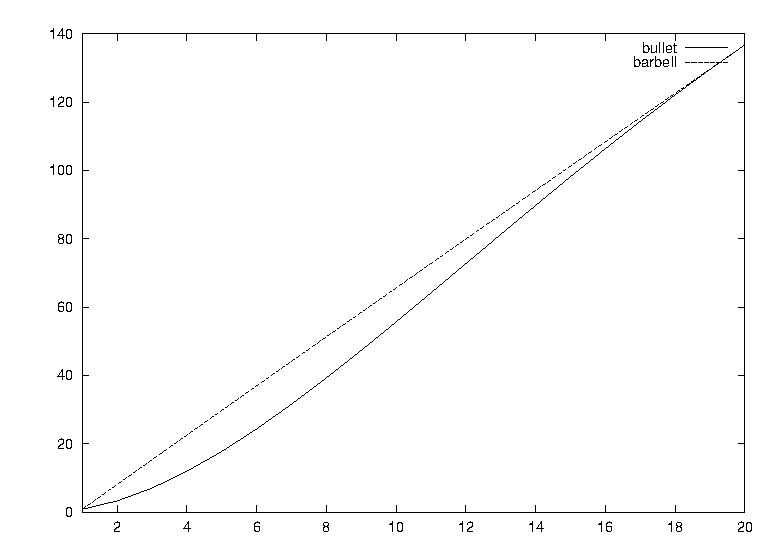
\includegraphics[scale=0.75]{bullet_vs_barbell.eps}
  \caption{Porovnání konvexity dvou portfólií se shodnou Macauleyovou durací sestrojených dle bullet resp. barbell strategie. Osa $x$ představuje duraci, osa $y$ konvexitu. Předpokládáme plochou výnosovou křivku na úrovni 5.00\%. Pro konstrukci portfolií byly použity diskontní dluhopisy.}
  \label{bullet_vs_barbell}
\end{figure}

Ladder strategie spočívá v investování shodné částky do dluhopisů s různou splatností. Tímto způsobem lze zkonstruovat portfolia, která mají odlišnou expozici na určitý segment výnosové křivky, a to v závislosti na zvolené splatnosti uvažovaných dluhopisů.

\subsubsection{Butterfly strategie}

Butterfly strategie je kombinací barbel strategie, která tvoří tzv. křídla, a bullet strategie, která tvoří tzv. tělo. Existuje celá řada různých typů butterfly strategií.

Butterfly strategie je často koncipována tak, aby výsledné portfolio mělo kladnou konvexitu při nulových počátečních nákladech a celkové dolarové duraci. To znamená, že portfolio generuje zisk za předpokladu paralelního posunu výnosové křivky. V případě změny sklonu popř. zakřivení výnosové křivky může však portfolio generovat výraznou ztrátu.\\

\noindent \textbf{Příklad:} Uvažujme plochou výnosovou křivku na úrovni 3.00\% a následující tři diskontní dluhopisy s nominální hodnotou 100 USD.
\begin{center}
\begin{tabular}{l l r r r r}
\textbf{Dluhopis} & \textbf{Splatnost}  & \textbf{Zero sazba} & \textbf{Cena} & \textbf{$D_{\$}$} & \textbf{$C_{\$}$}\\
\hline
A      & 1.0 rok   & 3.00\% &  97.182 &  -94.260 &   91.514\\
B      & 5.0 roky  & 3.00\% &  86.681 & -418.742 & 2032.729\\
C      & 10.0 roky & 3.00\% &  75.136 & -722.421 & 7013.799
\end{tabular}
\end{center}
Předpokládejme, že v dluhopisu B máme krátkou pozici -1~000 kusů. Abychom splnili podmínku nulových pořizovacích nákladů a nulové durace, musí být splněna rovnice
\begin{equation*}
\begin{bmatrix}
97.182 & 75.136 \\
-94.260 & -722.421
\end{bmatrix}
\begin{bmatrix}
q_1 \\
q_2
\end{bmatrix}
=
\begin{bmatrix}
86~681 \\
418~742
\end{bmatrix}
\end{equation*}
Řešením této rovnice je
\begin{equation*}
\begin{bmatrix}
q_1 \\
q_2
\end{bmatrix}
=
\begin{bmatrix}
493.604 \\
515.233
\end{bmatrix}
\end{equation*}
Výsledná hodnota portfolia je tedy nulová
\begin{equation*}
-1~000 \cdot 86.681 + (493.604 \cdot 97.087 + 515.233 \cdot 74.409) \approx 0
\end{equation*}
stejně jako durace.
\begin{equation*}
-1~000 \cdot -418.742 + (493.604 \cdot -94.260 + 515.233 \cdot -722.421) \approx 0
\end{equation*}
Konvexita tohoto portfolia je však kladná.
\begin{equation*}
-1~000 \cdot 2~032.729 + (493.604 \cdot 91.514 + 515.233 \cdot 7~013.799) \approx 1~626~183.023
\end{equation*}
To znamená, že portfolio generuje zisk jak pro paralelní růst tak pro paralelní pokles YTM. Například v případě pohybu o 0.1\% je výnos pro námi uvažované portfolio roven 0.813 USD.
\begin{equation*}
0.5 \cdot 1~626~183.023 \cdot 0.001^2 \approx 0.813
\end{equation*}
Přesným výpočtem získáváme 0.818 USD pro pokles a 0.808 USD pro růst YTM. $\clubsuit$\\

Vedle výše uvažované butterfly strategie je možné zkonstruovat portfolio s nulovou dolarovou durací tak, aby obě křídla měla shodnou duraci. Jestliže $q_1$ resp. $q_3$ představují počet dluhopisů tvořících první resp. druhé křídlo, $q_2$ počet dluhopisů tvořících tělo a $D_i$ příslušnou dolarovou duraci, musí platit
\begin{equation*}
\begin{bmatrix}
D_1 & D_3 \\
D_1 & -q_3 D_3
\end{bmatrix}
\begin{bmatrix}
q_1 \\
q_3
\end{bmatrix}
=
\begin{bmatrix}
q_2 D_2 \\
0
\end{bmatrix}
\end{equation*}
Řešením této lineární soustavy souřadnic je
\begin{equation*}
\begin{bmatrix}
q_1 \\
q_3
\end{bmatrix}
=
\begin{bmatrix}
D_1 & D_3 \\
D_1 & -q_3 D_3
\end{bmatrix}^{-1}
\begin{bmatrix}
q_2 D_2 \\
0
\end{bmatrix}
\end{equation*}
Uvažované portfolio je imunní vůči drobným paralelním posunům výnosové křivky a její rotaci kolem těla\footnote{Rotací kolem těla se rozumí změna sklonu výnosové křivky typu $(-x/0/x)$ resp. $(x/0/-x)$, kde první resp. třetí číslo vyjadřuje změnu na prvním resp. druhém křídle.}. Vzhledem k výše uvedeným podmínkám není tato podstrategie nákladově neutrální. Konstrukce portfolia tak může vyžadovat popř. generovat počáteční cash-flow.

Předchozí typ butterfly strategie vycházel z rovnoměného rozdělení dolarové durace mezi obě křídla. V praxi jsou však krátkodobé úrokové sazby více volatitní než dlouhodobé výnosové míry. Proto se YTM prvního křídla může od těla odchýlit více než YTM druhého křídla. Této skutečnosti více odpovídá nerovnoměrné rozložení dolarové durace mezi obě křídla, kdy větší díl připadne na první křídlo. Portfolio tak musí splňovat podmínky
\begin{equation*}
\begin{bmatrix}
D_1 & D_3 \\
D_1 & -\alpha q_3 D_3
\end{bmatrix}
\begin{bmatrix}
q_1 \\
q_3
\end{bmatrix}
=
\begin{bmatrix}
q_2 D_2 \\
0
\end{bmatrix}
\end{equation*}
kde $\alpha > 1$. Řešení má tak tvar
\begin{equation*}
\begin{bmatrix}
q_1 \\
q_3
\end{bmatrix}
=
\begin{bmatrix}
D_1 & D_3 \\
D_1 & -\alpha q_3 D_3
\end{bmatrix}^{-1}
\begin{bmatrix}
q_2 D_2 \\
0
\end{bmatrix}
\end{equation*}

Takto zkonstruované portfolio je imunní vůči rotaci typu $(-\alpha x/0/x)$ resp. $(\alpha x/0/-x)$.

Jestliže bychom chtěli měřit citlivost butterfly strategie na paralelní posun, změnu sklonu a zakřivení výnosové křivky, je možné použít Nelson-Siegelův model zero křivky. Hodnota portfolia je v rámci tohoto modelu dána rovnicí
\begin{equation*}
P_t = \sum_{i=1}^n F_i e^{-\theta_i R^c(t, \theta_i)}
\end{equation*}
kde $F_i$ představuje $i$-té cash-flow\footnote{Vzhledem k tomu, že butterfly strategie je založena na prodeji dluhopisů tvořících tělo a nákupu dluhopisů tvořících křídla, může být cash-flow $F_i$ jak kladné tak záporné.}. Citlivost portfolia na paralelní pohyb, změnu sklonu popř. zakřivení výnosové křivky je dána rovnicemi
\begin{equation*}
\frac{\partial P_t}{\partial \beta_0} = - \sum_{i=1}^n \theta_i F_i e^{-\theta_i R^c(t, \theta_i)}
\end{equation*}
\begin{equation*}
\frac{\partial P_t}{\partial \beta_1} = - \sum_{i=1}^n \theta_i F_i \Bigg( \frac{1 - e^{-\frac{\theta_i}{\tau}}}{\frac{\theta_i}{\tau}}\Bigg)e^{-\theta_i R^c(t, \theta_i)}
\end{equation*}
\begin{equation*}
\frac{\partial P_t}{\partial \beta_1} = - \sum_{i=1}^n \theta_i F_i \Bigg( \frac{1 - e^{-\frac{\theta_i}{\tau}}}{\frac{\theta_i}{\tau}} - e^{-\frac{\theta_i}{\tau}}\Bigg)e^{-\theta_i R^c(t, \theta_i)}
\end{equation*}
Vzhledem k tomu, že butterfly strategie má z definice nulovou dolarovou duraci, je $\frac{\partial P_t}{\partial \beta_0}$ blízké nule.

\subsection{Analýza scénářů}

Poněkud odlišným přístupem je poměřování zvolené investiční strategie pomocí scénářů možného vývoje výnosové křivky. Tyto scénáře mohou vycházet z historických dat, stochastického modelu popř. odrážet expertní odhad investora. Aplikace scénářů umožňuje analyzovat výkonnost strategie v různých tržních podmínkách a učinit si tak představu o nejlepší a nejhorší variantě vývoje.

Předpokládejme, že všechny uvažované scénáře jsou vyčerpávajícím přehledem možného budoucího vývoje výnosové křivky. Každému scénáři přiřaďme pravděpodobnost. Očekávanou výnosnost portfolia vypočíst jako vážený průměr výnosnosti portfolia pro jednotlivé scénáře, kde vahou je pravděpodobnost scénáře.

Ukažme si možnou aplikaci tohoto přístupu na Nelson-Siegelově modelu. Pro modelování zero sazeb jsou rozhodující parametry $\beta_0$, $\beta_1$ a $\beta_2$, na které je možné nahlížet jako na náhodné veličiny.
\begin{equation*}
\beta_i(t_j) = \beta_i(t_{j-1}) + \sigma_i X_i,~~~ i = 0, 1, 2
\end{equation*}
kde $X_i$ je výběr z náhodné veličiny s normovaným normálním rozdělením a $\sigma_i$ je historická směrodatná odchylka odpovídající časové periodě $t_j - t_{j-1}$. Dále je třeba zohlednit vzájemné korelace mezi jednotlivými parametry $\beta_i$. Empirické výzkumy ukázaly, že korelace mezi paralelními posuny a zakřivením je zanedbatelné. Parametry $\beta_0$ a $\beta_2$ je tak možné považovat za vzájemně nezávislé. Paralelní posuny a sklon křivky jsou pravděpodobně korelovány, nicméně se jedná o velmi slabou míru korelace. Z tohoto důvodu lze $\beta_0$ a $\beta_1$ považovat za vzájemně nezávislé. Naproti tomu sklon a zakřivení křivky vzájmně korelovány jsou. Tuto skutečnost je třeba zohlednit při generování $X_2$ a $X_3$. Vzájemně korelované veličiny lze modelovat následujícím způsobem. Nejprve definujme náhodnou veličinu $X_2$ jako
\begin{equation*}
X_2 = x_1
\end{equation*}
kde $x_1$ představuje výběr z normované normální náhodné veličiny. Korelovaná náhodná veličina $X_2$ je dána rovnicí
\begin{equation*}
X_3 = \rho x_1 + \sqrt{1 - \rho^2} x_2
\end{equation*}  
kde $\rho$ představuje požadovanou korelaci mezi $X_2$ a $X_3$ a $x_2$ je výběr z normované normální náhodné veličiny, která je nezávislá na $x_1$.

\subsection{Alokační strategie}

Empirickými pozorováními bylo prokázáno, že očekávaný výnos finančních aktiv je možné do určité míry předvídat. Pomocí sady vhodně vybraných veličin lze predikovat výnos pro odlišné typy finančních aktiv. Následně je změněna struktura portfolia ve prospěch finančních aktiv s nejvyšším predikovaným výnosem. Tento přístup nazýváme taktickou alokací aktiv (Tactical Assest Allocation - TAA). V 70. letech se TTA omezovala pouze na dvě třídy aktiv a to na dluhopisy a akcie. V současné době převažují strategie s podrobnějším členěním aktiv. V případě dluhopisů je nejběžnější definice skupin podle kreditního rizika.

\subsubsection{Volba faktorů sloužících k predikci}

Myšlenka, že různé typy aktiv mají různou výkonnost v různých fázích ekonomického cyklu, je intuitivní. Uvažujme tři kategorie dluhopisů - státních dluhopisů, korporátních dluhopisů s investičním ratingem a korporátních dluhopisů s neivestičních ratingem. Analýzou historických dat lze zjistit relativně malou korelaci mezi těmito skupinami. Je zřejmé, že čím vyšší je nejistota na trhu, tím více preferují investoři dluhopisy s vyšším ratingem. To lze poměrně názorně demonstrovat na vývoji tzv. kreditních spreadů\footnote{Uvažujme investora s dlouho pozicí v korporátním dluhopisu. Předpokládejme, že investor chce eliminovat kreditní riziko emitenta dluhopisu. K dluhopisu tak zakoupí tzv. kreditní swap. V rámci tohoto swapu platí na pravidelné bázi fixní částku, která se odvíjí od kreditního spreadu pro daného emitenta. V případě vzniku defaultní události emitenta má investor právo odprodat dluhopis za jeho nominální hodnotu. Kreditní swap má tak charakter pojištění a kreditní spready jsou tak vyjádřením tržní ceny rizika defaultu protistrany.}. Ty jsou relativně malé v době ekonomické konjunktury a relativně velké v době recese. Z tohotu důvodu je žádoucí v době konjunktury držet korporátní a v době recese státní dluhopisy. Zbývá tedy nalézt vhodné predikátory fáze tržního cyklu. V praxi se osvědčily následující finanční faktory
\begin{itemize}
\item tříměsíční výnosová míra státních podkladničních poukázek a dluhopisů - Fama (1981) a Fama a Schwert (1977) prokázali, že tato veličina je negativně korelována s budoucím vývojem na akciových trzích a lze ji tedy chápat jako indikátor očekávání budoucího ekonomického vývoje
\item dividendový výnos - tento ukazel plní úlohu predikátoru rizikové prémie, kdy vyšší dividendový výnos indikuje, že dividendy jsou diskontovány vyšší sazbou
\item ratingový spread (rozdíl mezi YTM dlouhodobých korporátních dluhopisů s nejvyšším a nejnižším investičním ratingem) - tento spread kopíruje tržní cyklus, kdy dosahuje vysokých resp. nízkých hodnot v době recese resp. konjunktury
\item časový spread (rozdíl mezi tříměsíčním a desetiletým výnosem ze státních dluhopisů)
\item implikovaná volatilita (kotovaná implikovaná volatilita pro opce na vybraný akciový index jako je např. VIX)
\item objem zobchodovaných transakcí na akciovém trhu
\item vývoj vybraného akciového indexu  
\end{itemize}
a ekonomické faktory
\begin{itemize}
\item inflace měřené růstem cen spotřebitele
\item peněžní nabídka vyjádřená ve formě peněžních agregátů
\item ekonomický růst ve formě čtvrtletního vývoje HDP
\end{itemize}
Praxe ukazuje, že korporátní dluhopisy s neinvestičním ratigem generují vyšší výnos než korporátní dluhopisy s investičním ratingem a státní dluhopisy, jestliže
\begin{itemize}
\item krátkodobé úrokové sazby jsou nízké a stabilní
\item dividendový výnos klesá popř. je stabilní
\item implikovaná volatilita výrazně klesá a akciový index roste
\item inflace je nízká a hospodářský růst vysoký
\end{itemize}
Pokud se zaměříme na výkonnost měřenou se zpožděním několika měsíců po analýze finančních a ekonomických faktorů, zjistili bychom, že vyššímu výnosu korporátních dluhopisů s neinvestičním ratingem předcházel(a)
\begin{itemize}
\item pokles krátkodobých úrokových sazeb navzdory nízké základně 
\item pokles dividendového výnosu
\item snížení kreditního spreadu z relativně vysokých výchozích hodnot
\item rostoucí výnosová křivka s vysokým sklonem
\item rostoucí objem zobchodovaných transakcí na akciovém trhu
\item vysoký výnos akciového indexu
\end{itemize}
V rámci TAA je tedy nutné sestrojit vhodný ekonometrický model, který bude predikovat vývoj ekonomického cyklu a na základě kterého budeme korigovat strukturu portfolia. Tento model zpravidla vychází z výše uvedených faktorů a je vhodné jej testovat na multikolinearitu\footnote{Multikolinearitou se rozumí situace, kdy jsou jednotlivé veličiny modelu korelované. To má za následek, že nelze oddělit vliv jedné z veličin od ostatních.} a heteroskedasticitu\footnote{Ekonometrické modely mají charakter regresních modelů - množinu historických pozorování chápeme jako body v $n$-rozměrném prostoru a snažíme se je proložit vhodnou křivkou. Je zřejmé, že tato aproximace pomocí křivky není dokonalá. Jinými slovy existuje rozdíl mezi reálně pozorozovanými daty a modelovanými daty. Tento rozdíl nazýváme statistickou chybou, která by měla chakter normální náhodné veličiny s nulovou střední hodnotou. Nesplnění této podmínky indikuje existenci systematické chyby v uvažovaném modelu - hovoříme o tzv. heteroskedasticitě.}. Při konstrukci modelu jsou historická data, která máme k dispozici, rozdělena na dvě části. Na větší části provádíme kalibraci modelu a na menší části pak testuje predikativní schopnosti modelu.

\section{Neefektivita trhu}

Hlavní myšlenkou investiční strategie založené na neefiktivitě trhu, je identifikace podhodnocených resp. nadhodnocených dluhopisů. Existují dva základní typy této investiční strategie a to
\begin{itemize}
\item investiční strategie, která se zaměřuje na jeden trh
\item investiční strategie, která se snaží těžit z neefektivity napříč trhy
\end{itemize}

\subsection{Neefektivity v rámci jednoho trhu}

Cílem této investiční strategie je identifikace dluhopisů, které jsou na daném trhu relativně k ostatním dluhopisům nadhodnocené resp. podhodnocené. Nadhodnocené dluhopisy jsou prodány a podhodnocené dluhopisy jsou nakoupeny. Existují dva rozdílné přístupy, které implementují investiční strategii založenou na neefektivitě v rámci jednoho trhu.
\begin{itemize}
\item První metoda je založena na porovnání dvou instrumentů, které jsou totožné z hlediska cash-flow. Klasickým případem je státní dluhopis a stripové dluhopisy, které vznikly jeho rozkladem.
\item Druhá metoda je založená na identifikaci dluhopisů, které jsou nadhodnoceny popř. podhodnoceny relativně k výnosové křivce.
\end{itemize}

\subsubsection{Státní dluhopis vs stripové dluhopisy}

Stripové dluhopisy jsou diskontní dluhopisy které vznikly rozkladem státního dluhopisu. Jednotlivé stripové dluhopisy odpovídají cash-flow generovanému podkladovým státním dluhopisem, který může být replikován pomocí těchto stripových dluhopisů. Teoretická cena dluhopisu je definována jako
\begin{equation}
P_t = \sum_{\substack{s = T - \alpha + 1} \\ s > 0}^T F_s B(t,s)
\end{equation}
kde $T$ je zbytková splatnost dluhopisu, $F_s$ cash-flow generované dluhopisem, $\alpha$ počet cash-flow generovaných dluhopisem a $B(t,s)$ představuje diskontní faktor. Cena státního dluhopisu by se měla rovnat součtu stripových dluhopisů, které vznikly jeho rozkladem. V opačném případě teoreticky existuje prostor pro arbitráž. Ve stutečnosti je situace poněkud složitější a to z důvodu rozdílné likvidity, která má podobu větších spreadů mezi bid a ask kotací. Omezený prostor pro arbitráž potvrzuje také studie, kterou provedl Jordan a kol. (2000) pro trh Spojených států.

\subsubsection{Cena dluhopisu vztažená k výnosové křivce}

Postup aplikovaný v rámci této investiční metody je následující. Ze skupiny homogenních dluhopisů zkonstruujeme zero křivku, kterou následně použijeme k výpočtu teoretické ceny uvažovaného dluhopisu. Z teoretické a skutečné ceny vypočteme YTM. Rozdíl mezi oběma YTM je indikátorem nadhodnocení resp. podhodnocení dluhopisu\footnote{V případě nadhodnoceného dlupisu je skutečný YTM menší než teoretický YTM. U podnodnoceného dluhopisu je tomu naopak.}.

K analýze rozdílu mezi skutečným a teoretickým YTM slouží tzv. Z-skórová analýza (Z-score analysis). Předpokládejme, že YTM spread má charakter náhodné veličiny s normálním rozdělením. Jestliže má spread ve zkoumané historické periodě, která má délku v řádu několika měsíců, střední hodnotu $m$ a směrodatnou odchylku $\sigma$, pak pro transformovanou náhodnou veličinu
\begin{equation*}
U = \frac{S - m}{2\sigma}
\end{equation*}
kde $S$ je aktuální YTM spread, platí
\begin{equation*}
P[-1 \le U \le 1] = 0.9544
\end{equation*}
Označme YTM spread jako $\hat{S}$ a odpovídající transformovanou náhodnou veličinu jako $\hat{U}$. Jestliže $\hat{U} > 1$, můžeme dluhopis považovat za podhodnocený. Bude-li $\hat{U} < - 1$, můžeme dluhopis považovat za nadhodnocený. 

Alternativně můžeme definovat spread $S_{min}$ resp. $S_{max}$, pro který je $\alpha$\% historických YTM spreadů nižší resp. vyšší než tento spread. Tento přístup tedy nepředpokládá, že YTM má charakter náhodné veličiny s normálním rozdělením a vychází z pravděpodonostního rozdělení, kterým se spread řídil v minulosti. Dále definujme transformovanou náhodnou veličinu
\begin{equation*}
U = \frac{S - S_{min}}{S_{max} - S_{min}}
\end{equation*}
V případě, že $U > 1$, lze daný dluhopis považovat za podhodnocený. Naopak $U < 0$ indikuje, že dluhopis je nadhodnocený.

Výše popsaná investiční strategie se zaměřuje na dluhopisy, jejichž aktuální YTM spread má ve vztahu k historickým datům charakter odlehlého pozorování. V souladu s touto strategií nakupujeme podhodnocené dluhopisy a nakrátko prodáváme nadhodnocené dluhopisy, přičemž při konstrukci portfolia je vhodné použít některou z imunizačních metod popsaných v kapitolách 5 a 6. Předpokladem uvažované investiční strategie je, že YTM spread bude konvergovat k dluhodobému historickému průměru. Pokud se tento předpoklad splní, je strategie zisková.

Investiční strategie založené na identifikaci nadhodnocených a podhodnocených dlupisů má řadu úskalí. Výběr dluhopisů, ze kterých bude vypočtena zero křivka, je třeba podřídit možným rozdílům z titulu odlišného profilu generovaného cash-flow\footnote{V první řadě je třeba, aby se jednalo o plain-vanilla dluhopisy bez vnořených opcí. Určité nepřesnosti mohou být způsobeny také rozdílnou frekvencí a výší kupónových sazeb.}, likvidity, ratingu atd. Dalším možným problémem je volba modelu výpočtu zero křivky. Také ceny dluhopisů, které vstupují do výpočtu zero křivky, nemusí, nejsou-li podepřeny skutečnými obchody, odpovídat skutečnosti. Na výsledek má také podstatný vliv délka historické periody, kterou použijeme pro výpočet historického YTM spreadu v rámci Z-skórové analýzy.

\subsection{Neefektivita napříč trhy}

Investiční strategie založené na využívání neefektivity napříč trhy jsou založeny na spreadových a konvergenčních obchodech.

\subsubsection{Spreadové obchody}

Uvažujme asset-swap. Tento typ obchodu se skládá ze dvou transakcí. Nejprve strana A koupí od strany B za par fixní dluhopis, jehož brutto cena je $P$. Současně strana A a B uzavřou úrokový swap. Strana A platí straně B pravidelně fixní platby, které kopírují cash-flow dluhopisu. Platby strany B straně A se odvíjí od referenční plovoucí sazby navýšené popř. ponížené o tzv. asset-swap spread. Asset-swap spread je stanoven tak, aby hodnota obchodu v okamžiku jeho sjednání byla rovna nule.

Stejně jako v předchozím případě lze pomocí Z-skórové analýzy identifikovat situace, kdy má asset-swap spread charakter odlehlého pozorování. Asset-swap spread mimojiné odráží zbytkovou splatnost dluhopisu a rating emitenta dluhopisu. Proto je třeba, aby délka historie, kterou použijeme pro kalibraci modelu, nepřesáhla několik málo měsíců a aby se během této doby nezměnil náhled trhu na kreditní riziko emitenta. Pokud by tyto podmínky nebyly splněny, byla by historická data nesouměřitelná. Z logiky věci vyplývá, že nízký asset-swap spread indikuje nadhodnocený dluhopis a naopak.

\subsubsection{Konvergenční obchody}

Jestliže se určitá země chystá vstoupit do měnové zóny, můžeme založit své obchody na předpokladu postupné konvergence úrokových sazeb popř. měnového kurzu k oficiálnímu zafixovanému kurzu platného v době konverze měny. Příkladem může být vstup Slovenské republiky do eurozóny, kdy na trhu prokazatelně existovaly arbitrážní příležitosti. Konvergenční obchody však lze obecně rozšířit na všechny situace, kdy na dvou oddělených trzích existují rozdíly, o kterých se investor domnívá, že časem zaniknou.

\chapter{Měření výkonnosti}

\section{Měření výnosové míry}

\subsection{Aritmetický průměr}

Uvažujme portfolio s hodnotou $V_t$ v čase $t$. Předpokládejme, že portfolio generuje v čase $t+1$ cash-flow $D_{t+1}$ a jeho hodnota těsně po výplatě cash-flow je rovna $V_{t+1}$. Výnosovou míru uvažovaného portfolia v rámci časové periody $t$ až $t+1$ lze vyjádřit jako
\begin{equation}
r_{t,t+1} = \frac{V_{t+1} - V_t + D_{t+1}}{V_t}
\end{equation}

Výnosová míra přes několik časových období je prostým součtem dílčích výnosových měr.
\begin{equation}
r_{t, t + n} = \sum_{i=1}^n r_{t + i - 1, t + i}
\end{equation}
Tento jednoduchý přístup definovaný rovnicí (9.2) však může vést k poměrně zavádějícím výsledkům.\\

\noindent \textbf{Příklad:} Uvažujme portfolio, jehož hodnota je v čase $t = 0$ rovna 100 USD, v čase $t = 1$ rovna 150 USD a v čase $t = 3$  rovna 100 USD. Předpokládejme, že portfolio v časové periodě $t = 0$ až $t=3$ negenerovalo žádné cash-flow.
Protože se hodnota portfolia v čase $t=0$ shoduje s hodnotou portfolia v čase $t=3$, je na první pohled zřejmé, že výnosová míra pro časovou periodu $t=0$ až $t=3$ je nulová.

Jestliže bychom však počítali celkovou výnosovou míru přes jednotlivé periody, byl by výsledek roven 16.667\%.
\begin{equation*}
\frac{150-100}{100} = 0.50000
\end{equation*}
\begin{equation*}
\frac{100-150}{150} \approx -0.33333
\end{equation*}
\begin{equation*}
0.50000 - 0.33333 = 0.16667
\end{equation*}
$\clubsuit$\\

Důvodem tohoto zkreslení je, že ve vzorci (9.2) neuvažujeme výnosy z reinvestovaných zisků a ztrát generovaných v jednotlivých časových subperiodách. Aritmetický průměr má totiž charakter jednoduchého úročení.\\

\noindent \textbf{Příklad:} Uvažujme stejné zadání jako v předchozím příkladě. Výnosová míra za časovou periodu $t=0$ až $t=2$ vypočtena na základě výnosových měr první a druhé subperiody je rovna 16.667\%. V čase $t=2$ bychom tak měli mít 116.67 USD. Předpokládejme, že zisk 50 USD generovaný na konci první subperiody reinvestujeme za výnosovou míru druhé subperiody. V čase $t=2$ tak máme 100 USD
\begin{equation*}
100 \cdot (1 + 0.16667) + 50 \cdot - 0.33333 \approx 100 
\end{equation*} 
čímž se dostáváme ke skutečné výnosové míře 0\%. $\clubsuit$\\

\subsection{Geometrický průměr}

Výše popsaný nedostatek odstraňuje geometrický průměr. Geometrický průměr existuje ve dvou variantách a to jako hodnotově a časově vážený.

V případě hodnotově váženéhé geometrického průměru lze výnosovou míru $r$ lze vypočíst z rovnice
\begin{equation*}
V_t = \sum_{i=1}^n \frac{F_{t+i}}{(1+r)^{t+i}} + \frac{V_{t+n}}{(1 + r)^{t+n}}
\end{equation*}
kde $F_{t+i}$ je cash-flow generované portfoliem v čase $t+i$ a $V_t$ resp. $V_{t+n}$ představují počáteční resp. konečnou hodnotu portfolia. Jedná se tedy o výnosovou míru do splatnosti.\\

\noindent \textbf{Příklad:} Uvažujme portfolio, jehož hodnota je v čase $t = 0$ rovna 102 USD a v čase $t=2$ rovna 113 USD. Předpokládejme, že v čase $t = 0.5$ portfolio generovalo cash-flow ve výši -5 USD. Výnosová míra vypočtená dle hodnotově váženého geometrického průměru je rovna 2.798\%.
\begin{equation*}
102 = \frac{-5}{(1+r)^{0.5}} + \frac{113}{(1+r)^2}
\end{equation*} 
$\clubsuit$\\

Konstrukce časově váženého geometrického průměru je v základních rysech podobná aritmetickému průměru. V prvním kroce je třeba zkoumanou periodu rozdělit podle generovaného cash-flow na subperiody a pro každou subperiodu vypočíst dle (9.1) výnosovou míru. Tento krok se shoduje postupem pro aritmetický průměr. V dalším kroce je třeba vypočíst celkovou výnosovou míru, která má charakter součinu dílčích výnosových měr přes jednotlivé časové subperiody.
\begin{equation*}
r_{t, t + n} = \prod_{i=1}^n (1 + r_{t + i - 1, t + i}) - 1
\end{equation*}

\noindent \textbf{Příklad:} Vraťme se zpět k příkladu zmiňovaného pro aritmetický průměr. Výnosová míra byla pro první subperiodu rovna 50.000\% a pro druhou subperiodu rovna -33.333\%. Celková výnosová míra dle časově váženého geometrického průměru je 0\%, což odpovídá skutečné výnosové míře.
\begin{equation*}
(1 + 0.50000)(1 - 0.33333) - 1 \approx 0.00000
\end{equation*}
$\clubsuit$\\

Hodnotově a časově vážená varianta geometrického průměru jsou shodné, jestliže ve zkoumané časové periodě negeneruje portfolio žádné cash-flow. V případě, že portfolio manažer nemá vliv vývoj cash-flow generovaného portfoliem\footnote{Klasickým příkladem mohou být pojišťovny, kdy je z portfolia vypláceno pojistné plnění. Cash-flow se tak odvíjí primárně od průběhu škodních události, které jsou zcela mimo vliv portfolio manažera.}, je vhodnější použít časově váženou variantu. Tato metoda totiž lépe eliminuje vliv rozdílného cash-flow v čase. V opačném případě se jako vhodnější jeví hodnotově vážený geometrický průměr. Tato varianta totiž zohledňuje snížení resp. navýšení objemu portfolia v návaznosti to, zda portfolio manažer očekává pokles resp. růst finančních aktiv tvořících portfolio.

\section{Zohlednění rizika}

Výnosovou míru portfolia je vhodné rozdělit na tzv. pasivní a aktivní složku. Pasivní složka odpovídá výnosu, který lze získat investování do indexu sloužícího jako srovnávací základna. Aktivní složka, kterou lze vypočíst jako rozdíl mezi skutečným výnosem a pasivní složkou, je ukazatelem kvalit portfolio manažera. Aktivní složku výnosu pak lze rozdělit na výnos, kterého bylo dosaženo vhodným načasováním obchodu a výnos, kterého se dosáhlo vhodnou volbou investičních instrumentů.

Měření výkonu portfolio manažera je poměrně složitý úkol, protože výnos musí být očištěn o riziko. K tomuto účelu je třeba zvolit vhodný benchmark. To znamená, že nejlepší portfolio manažer nemusí být nezbytně ten, který dosáhl nejvyššího výnosu.

\subsection{Absolutní výše rizika}

\subsubsection{Markowitz a Sharpeho poměr}

V roce 1952 přišel Markowitz s revoluční myšlenkou použít směrodatnou odchylku historických výnosů jako měřítko rizika investice.
\begin{equation*}
\sigma = \frac{1}{n} \sum_{t = 1}^n (R_t - \bar{R})^2
\end{equation*}
Na tomto pojetí rizika je založen tzv. Sharpeho poměr, který je nejznámějším vyjádřením výnosové míry očištěné o riziko. Sharpeho poměr je dán rovnicí
\begin{equation*}
sr = \frac{\bar{R} - r_f}{\sigma}
\end{equation*}
kde $r_f$ představuje bezrizikovou výnosovu míru.

Hlavní výhodou Sharpeho poměru je jeho jednoduchost a nezávislost na benchmarkovém indexu. Nevýhodou tohoto poměru je pak to, že pro kvantifikaci rizika používají první a druhý moment pravděpodobnostního rozdělení historických výnosů. Druhý a třetí moment nejsou brány v potaz, čímž může být ignorována velká část rizika. Klasickým případem jsou pravděpodobnostní rozdělení, které mají sice relativně malou směrodatnou odchylku, která je však kompenzována tzv. tlustými konci. Sharpeho poměr je tedy možné zkreslit tak, že pomocí vhodné investiční strategie přenese část rizika z druhého momentu na vyšší momenty\footnote{Lo (2001) se ve své studii zabýval investiční strategii založené na prodeji prodejních out-of-money opcí na S\&P 500 index se zbytkovou maturitou do tří měsíců. Tímto způsobem se mu podařilo pro časovou periodu leden 1992 až prosinec 1999 dosáhnout Sharpeho poměru 1.94 oproti 0.98 pro S\&P 500 index. Tato hodnota však byla vykompenzována výrazným nárůstem pravděpodobnosti extrémní ztráty. Ta se vázala právě na třetí a čtvrtý moment pravděpodobnostního rozdělení historických výnosových sazeb. Maximální denní ztráta generovaná touto strategií byla 18.3\% oproti 8.9\% pro index S\&P 500.}.

\subsubsection{Zohlednění vyšších momentů}

Jak již bylo zmíněno, Sharpeho index je založen pouze na střední hodnotě a směrodatné odchylce, které představují první a druhý moment pravděpodobnostního rozdělení. Je však možné nalézt taková dvě pravděpodobnostní rozdělení, která budou mít shodný první a druhý moment, ale budou se lišit v třetím resp. čtvrtém momentu, které označujeme jako sešikmení resp. zakřivení. Například kombinací normálního rozdělení se střední hodnotou 0.5 a smědatnou odchylkou 0.5 a normálního rozdělení se střední hodnotou -0.5 a směrodatnou odchylkou 1.32 získáme pravděpodobnostní rozdělení se střední hodnotu 0 a směrodatnou odchylkou 1. Normované normální rozdělení má taktéž střední hodnotu rovnu nule a směrodatnou odchylku rovnu jedné, nicméně sešikmení a zakřivení obou pravděpodobnostních rozdělení jsou odlišná. Situace je ilustrována obrázkem (\ref{probability_distribution}).
\begin{figure}
  \centering
  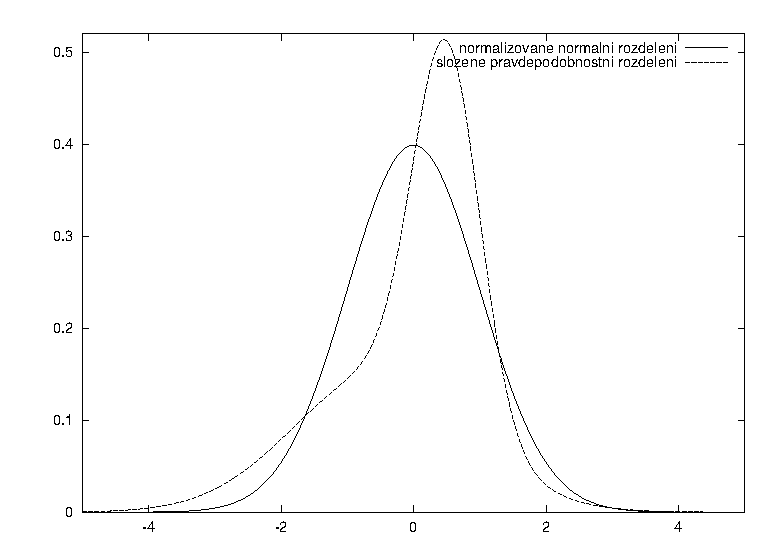
\includegraphics[scale=0.75]{probability_distribution.eps}
  \caption{Normalizované normální rozdělení a pravděpodobnostní rozdělení vzniklé složením dvou normálních rozdělení - obě pravděpodobnostní rozdělení mají shodné první dva momenty, avšak liší se druhým a třetím momentem}
  \label{probability_distribution}
\end{figure}

V případě třetího momentu, tj. šikmosti, je standardním ukazatelem rizika tzv. semivariance
\begin{equation*}
\sigma^{-} = \frac{1}{T^{-}} \sum_{t \Rightarrow R_t \le \bar{R}} (R_t - \bar{R})^2
\end{equation*}
kde $T^{-}$ představuje počet výnosových měr nižších než průměrná výnosová míra. Definujme tzv. minimální přijatelnou výnosovou míru MAR, která ve výše uvedené rovnici nahradí $\hat{R}$. Pomocí MAR tak lze definovat analogii k Sharpově poměru nazývanou Sortinovým poměrem.
\begin{equation*}
sor = \frac{\bar{R} - \mathrm{MAR}}{\sqrt{\frac{1}{T^{\mathrm{MAR}}}\sum_{t \Rightarrow R_t \le \mathrm{MAR}}(R_t - \mathrm{MAR})^2}}
\end{equation*}

Chceme-li zohlednit čtvrtý moment, musíme nejprve vypočíst hodnotu VaR. Nejprve je třeba definovat pravděpodobnostní rozdělení zisků a ztrát uvažovaného portfolia v průběhu dané časové periody. S jeho pomocí jsme schopni odpovědět na otázku, jaká je ztráta, která nebude s pravděpodobností $x$\% překročena. Tuto pseudomaximální ztrátu nazýváme VaR (Value-at-Risk). Standardně se výše VaR počítá pro 95\% resp. 99\% pravděpodobnost a pro časovou periodu jednoho, pěti nebo deseti pracovních dní. Hodnotu VaR je možné vypočíst
\begin{itemize}
\item pomocí historické metody - V případě této metody je nejprve zvolena historická časová perioda. Pro každý den periody je definován scénář daný změnou úrokových sazeb pro tento den. Tyto scénáře slouží jako vstup pro ocenění uvažovaného portfolia, čímž pro každý den získáme hypotetickou hodnotu portfolia. S jejich pomocí jsme schopni odvodit pravděpodobnostní rozdělení ztrát a ztrát a následně vypočíst jednodenní VaR.
\item analyticky - V případě analytického přístupu je snahou odvodit z pravděpodobnostních rozdělení jednotlivých rizikových faktorů složené pravděpodobnostní rozdělení zisků a ztrát uvažovaného portfolia. Za tímto účelem je však nutné aplikovat řadu aproximací, které mohou výsledný VaR zkreslit.
\item metodou Monte-Carlo - Metoda Monte-Carlo je založena na definování pravděpodobnostního rozdělení jednotlivých rizikových faktorů a jejich následné simulaci. Výsledky simulace následně slouží jako vstup pro oceňovací model portfolia. V každém kole simulace tak získáme hypotetický zisk popř. ztrátu. Na jejich základě lze zkonstruovat empirické pravděpodobnostní rozdělení a následně vypočíst hodnotu VaR.
\end{itemize}
V případě, že jsme aplikací některé z výše uvedených metod vypočetli hodnotu VaR, je možné modifikovat rovnici Sharpova poměru.
\begin{equation*}
sr_m = \frac{\bar{R}-r_f}{|\mathrm{VaR}|}
\end{equation*}

Žádný z výše uvedených poměrových ukazatelů nezohledňoval výkonnost relativně k benchmarku. Uvažujme portfolio státních dluhopisů a portfolio korporátních dluhopisů. Předpokládejme, že procentní růst indexu státních dluhopisů byl vyšší než procentní růst hodnoty prvního portfolia. Dále předpokládejme, že současně s tím index koprorátních dluhopisů klesl, však tento pokles byl výraznější než byl pokles hodnoty druhého portfolia. Protože první portfolio generovalo zisk a druhé ztrátu, preferují všechny poměrové ukazatele první z nich. Jestliže bychom však brali v potaz výkonnost benchmarku, bylo by lépe hodnoceno druhé portfolio.

\subsection{Relativní výše rizika}

S ohledem na výše uvedenou poznámku je žádoucí hodnotit výkonnost portfolia relativně ve vztahu k vhodně zvolenému benchmarku.

\subsubsection{Faktorové modely}

Faktorové modely jsou založeny na myšlence, že existují zdroje rizika a že expozice vůči těmto rizikům generuje výnos nad rámec bezrizikové úrokové sazby. Tento přístup nám umožňuje rozdělit výnos portfolia na
\begin{itemize}
\item normální výnos, který odpovídá bechmarku a představuje tak kompenzaci za podstupovaná rizika
\item a výnos nad rámec výnosu benchmarku, který lze považovat za odraz schopností portfolio manažera
\end{itemize}
Hlavním problémem tohoto přístupu je definice "normálního" výnosu.

Obecný tvar faktorových modelů je
\begin{equation}
\alpha = \bar{r} - r_f - \sum_{k=1}^K \beta_{k}\lambda_k
\end{equation}
kde $\alpha$ je rizikově očištěný výnos portfolia, $\bar{r}$ průměrný výnos portfolia, $r_f$ bezriziková výnosová míra, $\beta_{ik}$ expozice portfolia vůči $k$-tému rizikovému faktoru a $\lambda_k$ představuje rizikovou prémii $k$-tého rizikového faktoru. Omezením (9.3) na jeden rizikový faktor získáváme známý CAPM model
\begin{equation*}
\alpha = \bar{r} - r_f - \beta(\bar{r_M} - r_f)
\end{equation*}
kde $\bar{r_M}$ představuje průměrný výnos tržního portfolia aproximovaného dostatečně širokým indexem, $\beta$ je expozice portfolia vůči riziku trhu, jehož cena je $\lambda = \bar{r_M} - r_f$. Jeden rizikový faktor, jakým je v případě modelu CAMP expozice vůči tržnímu portfoliu, se v praxi ukázal jako nedostatečný. Tím se dostáváme ke klíčovému problému rovnice (9.3), kterým je volba rizikových faktorů. S ohledem na tuto problematiku je možné rozlišit tři typy faktorových modelů.
\begin{itemize}
\item Implicitní faktorový model - Tento přístup je založen na vektorové dekompozici, která slouží k získání rizikových faktorů z historické řady výnosových měr. Tento přístup je po statistické stránce robustní a odstraňuje případné problémy se zahrnutím pseudofaktorů popř. opomenutím důležitých faktorů. Nadruhou stranu takto získané rizikové faktory zpravidla nemají jednoduchou ekonomickou interpretaci.
\item Makrofaktorový model - V této verzi modelu jsou jako faktory použity makroekonomické veličiny jako např. míra inflace, růst průmyslové výroby doplněné o finanční veličiny jako např. spread mezi výnosy státních a korporátních dluhopisů, spread mezi krátkodobými a dlouhodobými státními dluhopisy.
\item Faktorový model založený na indexech - V rámci tohoto typu modelu jsou jako rizikové faktory použity tržní indexy. Do této kategorie patří také výše uváděný model CAMP a model French-Fama (1992). 
\end{itemize}

\subsubsection{Dluhopisové indexy jako vstup faktorového modelu}

Vraťme se zpět k faktorovému modelu založeném na indexech. V případě dluhopisového portfolia by jako rizikové faktory mohly vystupovat dluhopisové indexy, které by odrážely složení portfolia. Aby bylo možné dluhopisový index považovat za vhodného kandidáta, měl by být
\begin{itemize}
\item respektovaný - index by měl být všeobecně přijímán jako benchmarkový
\item reprezentativní pro daný segment trhu - index musí odrážet skutečné investiční příležitosti daného segmentu
\item replikovatelý - měla by existovat praktická možnost replikovat tento index pomocí pasivní investiční strategie
\item stabilní a transparentní - musí existovat přesná a srozumitelná pravidla pro výpočet hodnoty indexu a změnu jeho složení
\end{itemize}

Existuje celá řada dluhopisových indexů, které pokrývají různé segmenty dluhopisového trhu. Mezi všeobecně používáné dluhopisové indexy patří
\begin{itemize}
\item Barclays Capital Bond Composite Global Index, který reprezentuje globální dluhopisový trh
\item Barclays Capital Aggregate Bond Index pro globální dluhopisový trh Spojených států (zahrnuje státní, municipální a korporátní dluhopisy s investičním ratingem)
\item J.P. Morgan EMBI index pro dluhopisy rozvojových trhů 
\item J.P. Morgan Government Bond Index a Salomon Smith Barney World Government Bond Index zaměřené na globální trh státních dluhopisů
\item EuroMTS New EU Goverment Bond Index pro státní dluhopisy zemí eurozóny
\item Dow Jones Corporate Bond Index pro korporátní dluhopisy Spojených států s vysokým ratingem
\end{itemize}

V případě, že se portfolio prolíná několika segmenty dluhopisového trhu, nemusí být veřejně dostupné dluhopisové indexy vhodným benchmarkem. Řešením tohoto problému je úprava báze existujícího indexu tak, aby odpovídal požadované investiční strategii. Úprava báze spočívá v přidání popř. vyřazení dluhopisů a změny jejich váhy v indexu. Takto upravené indexy pak mohou být použity jako vstup pro modifikaci rovnice (9.3)
\begin{equation*}
\alpha = \bar{r} - r_f - \sum_{k=1}^K \beta_k (\bar{r_k} - r_f)
\end{equation*}
kde $\beta_k$ představuje expozici portfolia vůči $k$-tému dluhopisovému indexu a $\bar{r_k}$ je průměrná výnosová míra $k$-tého indexu.

Alternativou k faktorovému modelu je rozdělení portfolio podle segmentu dluhopisového trhu, nalezení odpovídajícího dluhopisového indexu pro každý tento segment a výpočet výsledného benchmarku jako váženého průměru těchto indexů. Benchmarkový výnos $r_B$ má tak podobu
\begin{equation*}
r_B = \sum_{k=1}^K w_k I_k
\end{equation*}
kde $I_k$ je dluhopisový index reprezentující $k$-tý segment dluhopisového trhu a $w_k$ představuje váhu $k$-tého segmentu dluhopisového trhu v rámci portfolia.

\part{Swapy a futures}

\chapter{Swapy}

\section{Plain-vanilla úrokový swap}

\subsection{Definice}

Plain-vanilla úrokový swap je transakcí mezi dvěma subjekty na trhu, která je charakteristická
\begin{itemize}
\item pravidelnými směnami
     \begin{itemize}
     \item plateb odvozených od fixní úrokové sazby
     \item za platby odvozené od referenční pohyblivé úrokové sazby (např. šestiměsíční Libor),
     \end{itemize}
\item kde výše směňovaného cash-flow je odvozena od frekvence úročení a výše podkladoveného nominálu,
\item přičemž frekvence úročení pohyblivých plateb je dána splatností referenční pohyblivé úrokové sazby,
\item frekvence úročení pevných a pohyblivých plateb se nemusí shodovat,
\item výše podkladového nominálu je konstantní po celou dobu trvání úrokového swapu,
\item a podkladový nominál není předmětem směny.
\end{itemize} 
\begin{center}
  \begin{pspicture}(0,0)(8.0,5.5)
        \rput(4.0,1.3){Plain-vanilla úrokový swap se splatností tří let: investor}
	\rput(4.0,0.9){platí jednou ročně fixní platby ve výši 4.00\% p.a. a každého}
	\rput(4.0,0.5){půl roku obdrží pohyblivé platby odpovídající 6M Libor}

	\psline(0.3,4.0)(7.7,4.0)

	\psline(0.5,3.9)(0.5,4.1)

	\psline[linestyle=dashed,arrows=->](1.5,4.0)(1.5,5.0)
	\psline[linestyle=dashed,arrows=->](2.5,4.0)(2.5,5.0)
	\psline[linestyle=dashed,arrows=->](3.5,4.0)(3.5,5.0)
	\psline[linestyle=dashed,arrows=->](4.5,4.0)(4.5,5.0)
	\psline[linestyle=dashed,arrows=->](5.5,4.0)(5.5,5.0)
	\psline[linestyle=dashed,arrows=->](6.5,4.0)(6.5,5.0)

	\psline[arrows=->](2.5,4.0)(2.5,2.0)
	\psline[arrows=->](4.5,4.0)(4.5,2.0)
	\psline[arrows=->](6.5,4.0)(6.5,2.0)

	\rput(0.5,3.8){\tiny{0}}
	\rput(1.7,3.8){\tiny{6M}}
	\rput(2.7,3.8){\tiny{1Y}}
	\rput(3.7,3.8){\tiny{1.5Y}}
	\rput(4.7,3.8){\tiny{2Y}}
	\rput(5.7,3.8){\tiny{2.5Y}}
	\rput(6.7,3.8){\tiny{3Y}}

	\rput(0.5,5.0){\tiny{6M Libor}}
	\rput(0.5,2.3){\tiny{4.00\%}}

  \end{pspicture}
\end{center}
Pevné platby nazýváme fixní a pohyblivé platby floatovou nohou úrokového swapu. Uvažujme fiktivní směnu nominálů na konci životnosti úrokového swapu. Vzhledem k tomu, že podkladový nominál je shodný pro obě nohy, nemá tento předpoklad vliv na hodnotu úrokového swapu\footnote{Každá strana s poslední platbou zaplatí a zároveň obdrží podkladový nominál. Tato zdánlivě iracionální transakce má tedy nulový dopad do hodnoty úrokového swapu.}. Po této úpravě má plain-vanilla úrokový swap stejný profil cash-flow jako portfolio složené z jednoho fixního a jednoho floatového dluhopisu. Tento poznatek je klíčem k ocenění úrokového swapu.

\subsection{Ocenění}

Úrokový swap je možné chápat jako směnu fixního a floatového dluhopisu, které reprezentují fixní a floatovou nohu. Hodnota úrokového swapu je dána součtem hodnoty fixní a floatové nohy. V okamžiku sjednání obchodu mají obě nohy zpravidla stejnou hodnotu, což implikuje nulovou hodnotu swapu. S tím, jak se v průběhu životnosti swapu mění struktura úrokových sazeb, mění se také jeho hodnota. Fixní noha má v porovnání s floatovou nohou vyšší duraci, a proto její hodnota reaguje na změnu úrokových sazeb výrazněji.

Hodnota fixní nohy je rovna současné hodnotě jejího cash-flow. Veškeré cash-flow fixní nohy lze jednoznačně určit v okamžiku uzavření obchodu. Jestliže máme k dispozici výnosovou křivku, je její ocenění triviální záležitostí. 

V případě floatové nohy je situace složitější. Výše platby pro aktuální úrokové období se odvozuje od referenční úrokové sazby na začátku tohoto období. To znamená, že v libovolném časovém okamžiku známe pouze hodnotu nejbližšího cash-flow. Zbylá cash-flow se odvíjí od budoucích hodnot referenční úrokové sazby, a proto nejsou dopředu známa. Za předpokladu neexistence arbitráže lze budoucí hodnoty referenční sazby odhadnout pomocí odpovídajích forwardových úrokových sazeb.

\subsubsection{Přesný tvar rovnice výpočtu hodnoty úrokového swapu}

Z pohledu investora, který hradí platby z floatové nohy a obdrží platby z fixní nohy, je hodnota plain-vanilla úrokového swapu rovna
\begin{equation}
\mathrm{MV}_t^{\mathrm{swap}} = N \Bigg( \sum_{i=1}^n I^{\mathrm{fix}} \frac{T_i^{\mathrm{fix}}-T_{i-1}^{\mathrm{fix}}}{360}B(t,T_i^{\mathrm{fix}}) - \sum_{j=1}^m I_{j-1}^{\mathrm{fwd}} \frac{T_j^{\mathrm{float}}-T_{j-1}^{\mathrm{float}}}{360}B(t,T_j^{\mathrm{float}}) \Bigg)
\end{equation}
kde
\begin{center}
\begin{tabular}{l l}
$N$ & je výše podkladového nominálu úrokového swapu\\
$n$ & je počet plateb generovaných fixní nohou od časového okamžiku $t$ do\\
    & splatnosti úrokového swapu v čase $T_n^{\mathrm{fix}}$\\
$m$ & je počet plateb generovaných floatovou nohou od časového okamžiku $t$ do\\
    & splatnosti úrokového swapu v čase $T_m^{\mathrm{float}}$ (z toho vyplývá $T_n^{\mathrm{fix}} = T_m^{\mathrm{float}}$)\\
$T_i^{\mathrm{fix}}$ & je datum, ke kterému je vyplaceno $i$-té cash-flow fixní nohy;\\
                     & $T_0^{\mathrm{fix}}$ představuje datum, od kterého začala nabíhat aktuální platba\\
$T_j^{\mathrm{float}}$ & je datum, ke kterému je vyplaceno $j$-té cash-flow floatové nohy;\\
                       & $T_0^{\mathrm{float}}$ představuje datum, od kterého začala nabíhat aktuální platba\\
$T_{i} - T_{i-1}$ & je počet kalendářních dní mezi $i$-tou a $(i-1)$-tou platbou\\      
$I^{\mathrm{fix}}$ & je fixní úroková sazba, která slouží k výpočtu plateb generovaných fixní nohou\\
$I_{j-1}^{\mathrm{fwd}}$ & je forwardová úroková sazba, která slouží jako odhad budoucí hodnoty\\
                         & referenční úrokové sazby pro časové období $T_{j-1}^{\mathrm{float}}$ až $T_j^{\mathrm{float}}$;\\
                         & $I_0^{\mathrm{fwd}}$ je hodnota referenční sazby, podle které byla vypočtena výše aktuálně\\
                         & nabíhající platby (tj. tato hodnota byla pozorovatelná v minulosti v čase $T_0^{\mathrm{float}}$)\\
$B(t,T_i)$      & je diskontní faktor pro časový interval od $t$ do $T_i$\\
\end{tabular}
\end{center}

\subsubsection{Zjednodušený tvar rovnice výpočtu hodnoty úrokového swapu}

Nejbližší cash-flow floatové nohy úrokového swapu je vypláceno v čase $T_1^{\mathrm{float}}$. Hodnotu tohoto cash-flow známe. Hodnoty cash-flow vyplácených po tomto datu neznáme - můžeme je pouze odhadovat pomocí forwardových sazeb.

Uvažujme výše popisovanou fiktivní směnu podkladového nominálu v době splatnosti úrokového swapu. Výpočet forwardových sazeb a diskontních faktorů je prováděn na základě téže výnosové křivky. Proto je hodnota cash-flow floatové nohy vyplácená po $T_1^{\mathrm{float}}$ diskontovaná k témuž data rovna hodnotě podkladového nominálu. Celková hodnota floatové nohy je tak rovna současné hodnotě nejbližší platby navýšené o hodnotu podkladového nominálu diskontované k $T_1^{\mathrm{float}}$. Výpočet hodnoty fixní nohy se v zásadě nezměnil - pouze musíme zohlednit fiktivní směnu podkladového nominálu v době splatnosti úrokového swapu. Rovnice (10.1) se tak zjednoduší do tvaru
\begin{equation}
\mathrm{MV}_t^{\mathrm{swap}} = N \Bigg( \sum_{i=1}^n I^{\mathrm{fix}} \frac{T_i^{\mathrm{fix}}-T_{i-1}^{\mathrm{fix}}}{360}B(t,T_i^{\mathrm{fix}}) + B(t, T_n^{\mathrm{fix}}) - (1 + I_0^{\mathrm{fwd}}\frac{T_1^{\mathrm{float}} - T_0^{\mathrm{float}}}{360})B(t,T_1^{\mathrm{float}}) \Bigg)
\end{equation}

Lze snadno dokázat, že rovnice (10.1) a (10.2) jsou ekvivalentní. Hodnota floatové nohy dle (10.1) je rovna
\begin{equation*}
\mathrm{MV}_t^{\mathrm{float~leg}} = \sum_{j=1}^m I_{j-1}^{\mathrm{fwd}} \frac{T_j^{\mathrm{float}}-T_{j-1}^{\mathrm{float}}}{360}B(t,T_j^{\mathrm{float}})
\end{equation*}
Tuto rovnici upravme do tvaru, který zahrnuje fiktivní směnu nominálu na konci splatnosti úrokového swapu.
\begin{equation}
\mathrm{MV}_t^{\mathrm{float~leg*}} = N \Bigg(I_0^{\mathrm{fwd}} \frac{T_1^{\mathrm{float}}-T_0^{\mathrm{float}}}{360}B(t,T_1^{\mathrm{float}}) + \sum_{j=2}^m I_{j-1}^{\mathrm{fwd}} \frac{T_j^{\mathrm{float}}-T_{j-1}^{\mathrm{float}}}{360}B(t,T_j^{\mathrm{float}}) + B(t,T_m^{\mathrm{float}}) \Bigg)
\end{equation}
kde $I_0^{\mathrm{fwd}}$ je hodnota referenční pohyblivé úrokové sazby z času $T_0^{\mathrm{float}} \le t$. Forwardová sazba $I_{j-1}^{\mathrm{fwd}}$ je definována jako
\begin{equation*}
I_{j-1}^{\mathrm{fwd}} = \Bigg( \frac{B(t,T_{j-1}^{\mathrm{float}})}{B(t,T_j^{\mathrm{float}})} - 1 \Bigg) \frac{360}{T_j^{\mathrm{float}} - T_{j-1}^{\mathrm{float}}}
\end{equation*}
Dosazením do (10.3) a následnými úpravami získáme
\begin{equation*}
\mathrm{MV}_t^{\mathrm{float~leg*}} = N \Bigg(I_0^{\mathrm{fwd}} \frac{T_1^{\mathrm{float}} - T_0^{\mathrm{float}}}{360}B(t,T_1^{\mathrm{float}}) + \sum_{j=2}^m \Big( B(t,T_{j-1}^{\mathrm{float}}) - B(t,T_j^{\mathrm{float}}) \Big) + B(t,T_m^{\mathrm{float}}) \Bigg)
\end{equation*}
\begin{equation}
\mathrm{MV}_t^{\mathrm{float~leg*}} = N \Bigg(1 + I_0^{\mathrm{fwd}} \frac{T_1^{\mathrm{float}} - T_0^{\mathrm{float}}}{360} \Bigg)B(t,T_1^{\mathrm{float}})
\end{equation}
Hodnota fixní nohy včetně fiktivní směny nominálu na konci splatnosti úrokového swapu je rovna
\begin{equation}
\mathrm{MV}_t^{\mathrm{fix~leg*}} = N \Bigg( \sum_{i=1}^n I^{\mathrm{fix}} \frac{T_i^{\mathrm{fix}}-T_{i-1}^{\mathrm{fix}}}{360}B(t,T_i^{\mathrm{fix}}) +  B(t,T_n^{\mathrm{fix}})\Bigg)
\end{equation}
Sloučením (10.4) a (10.5) získáme (10.2). Tímto jsme dokázali, že rovnice (10.1) a (10.2) jsou identické.

Pro $T_0^{\mathrm{float}} = t$ je hodnota floatové nohy, za předpokladu fiktivní směny nominálu, rovna podkladovému nominálu úrokové swapu. V tomto případě je totiž $I_0^{\mathrm{fwd}}$ rovno depozitní sazbě pro období $t$ až $T_1^{\mathrm{float}}$ a diskotní faktor $B(t,T_1^{\mathrm{float}})$ je tak definován jako
\begin{equation*}
B(t,T_1^{\mathrm{float}}) = B(T_0^{\mathrm{float}},T_1^{\mathrm{float}}) = \frac{1}{1 + I_0^{\mathrm{fwd}}\frac{T_1^{\mathrm{float}}-T_0^{\mathrm{float}}}{360}}
\end{equation*}
Dosazením do (10.2) se tak tato rovnice dále zjednoduší do tvaru
\begin{equation}
\mathrm{MV}_t^{\mathrm{swap}} = N \Bigg( \sum_{i=1}^n I^{\mathrm{fix}} \frac{T_i^{\mathrm{fix}}-T_{i-1}^{\mathrm{fix}}}{360}B(t,T_i^{\mathrm{fix}}) +  B(t,T_n^{\mathrm{fix}}) - 1\Bigg)
\end{equation}
\\

\noindent \textbf{Příklad:} Uvažujme plain-vanilla úrokový swap s podkladovým nominálem 1~000~000 CZK a splatností tři roky, jehož fixní úroková sazba je 2.83\% a jako pohyblivá referenční sazba je zvolen šestiměsíční Pribor. Frekvence úročení fixní i floatové nohy je půl roku. Výnosová křivka je dána níže uvedenou tabulkou.
\begin{center}
     \begin{tabular}{|c c | c c c c|}
     \cline{1-6}
     \textbf{Datum} & \textbf{Datum} & \textbf{Par} & \textbf{Diskontní} & \textbf{Zero} & \textbf{6M forwardová} \\
     \textbf{ocenění} & \textbf{výplaty} & \textbf{sazba} & \textbf{faktor} & \textbf{sazba} & \textbf{sazba} \\
     \hline
     25/11/2009 & 25/05/2010 & 2.00\% & 99.00446\% & 2.03814\% & 2.27468\% \\
     25/11/2009 & 25/11/2010 & 2.15\% & 97.86664\% & 2.17986\% & 2.78667\% \\
     25/11/2009 & 25/05/2011 & 2.35\% & 96.51440\% & 2.40004\% & 2.95784\% \\
     25/11/2009 & 25/11/2011 & 2.50\% & 95.07705\% & 2.55626\% & 3.79384\% \\
     25/11/2009 & 25/05/2012 & 2.75\% & 93.28779\% & 2.81979\% & 3.80718\% \\
     25/11/2009 & 25/11/2012 & 2.92\% & 91.50716\% & 2.99985\% & 3.29132\% \\
     25/11/2009 & 25/05/2013 & 2.97\% & 90.01755\% & 3.05154\% & \\
     \cline{1-6}
     \end{tabular}
\end{center}
Následující tabulka představuje ocenění úrokového swapu dle (10.1), tj. z pohledu investora, který platí cash-flow floatové nohy a obdrží cash-flow fixní nohy. Výsledná hodnota úrokového swapu je -2~617.66 CZK.
\begin{center}
     \begin{tabular}{|c | c c | c c|}
     \cline{1-5}
      & \multicolumn{2}{c|}{\textbf{Fixní noha}} & \multicolumn{2}{c|}{\textbf{Floatová noha}} \\
     \textbf{Datum} &  \textbf{Fixní} & \textbf{Diskontované} & \textbf{Forwardová} & \textbf{Diskontované} \\
     \textbf{výplaty} &  \textbf{sazba} &\textbf{cash-flow} & \textbf{sazba} & \textbf{cash-flow} \\
     \hline
     25/05/2010   & 2.83\% & 14,086.96 & 2.00000\% &  -9,955.45 \\
     25/11/2010   & 2.83\% & 14,155.87 & 2.27468\% & -11,378.12 \\
     25/05/2011   & 2.83\% & 13,732.66 & 2.78667\% & -13,522.40 \\
     25/11/2011   & 2.83\% & 13,752.37 & 2.95784\% & -14,373.58 \\
     25/05/2012   & 2.83\% & 13,346.89 & 3.79384\% & -17,892.55 \\
     25/11/2012   & 2.83\% & 13,236.00 & 3.80718\% & -17,806.30 \\
     \hline
     Hodnota nohy &         & 82,310.74 &           & -84,928.40 \\
     \hline
     Celková hodnota &        \multicolumn{3}{c}{}       & -2,617.66 \\
     \cline{1-5}
     \end{tabular}
\end{center}
Hodnota fixní nohy včetně fiktivní výměny nominálu na konci splatnosti úrokového swapu je 997~382.34 CZK.
\begin{equation*}
\sum_{i=1}^n I^{\mathrm{fix}} \frac{T_i^{\mathrm{fix}}-T_{i-1}^{\mathrm{fix}}}{360}B(t,T_i^{\mathrm{fix}}) + B(t, T_n^{\mathrm{fix}}) = 82~310.74 + 1~000~000 \cdot 0.9150716 = 997~382.34
\end{equation*}
Jestliže bychom použili pro výpočet hodnoty úrokového swapu rovnici (10.2), získáme
\begin{equation*}
997~382.34 - 1~000~000 \cdot (1 + 0.02 \cdot 0.50278) \cdot 0.9900446 = -2~617.66
\end{equation*}
Obě metody výpočtu hodnoty úrokového swapu tedy vedou ke shodnému výsledku.

Protože se den ocenění swapu shoduje s prvním dnem aktuálního úrokového období pro floatovou nohu, nebo-li $T_0^{\mathrm{float}} = t$, měla by být hodnota swapové nohy rovna hodnotě podkladového nominálu. Také tato podmínka je splněna.
\begin{equation*}
N \sum_{j=1}^m I_{j-1}^{\mathrm{fwd}} \frac{T_j^{\mathrm{float}}-T_{j-1}^{\mathrm{float}}}{360}B(t,T_j^{\mathrm{float}}) +  N \cdot B(t,T_m^{\mathrm{float}}) = 84~928.40 + 1~000~000 \cdot 0.9150716 = 1~000~000
\end{equation*}
$\clubsuit$

\subsection{Tržní kotace}

Cena úrokového swapu, za kterou jsou subjekty na trhu ochotny uzavřít s protistranou obchod, je kotována ve formě pevné sazby pro fixní nohu. Tato tzv. swapová sazba definována měnou, splatností úrokového swapu a pohyblivou referenční úrokovou sazbu včetně frekvence úročení floatové nohy. Swapová sazba je nastavena tak, aby se hodnota pevné nohy za předpokladu roční frekvence úročení rovnala hodnotě floatové nohy.

\begin{figure}
  \includegraphics[bb=0 0 350 250]{irs_czk.bmp}
  \caption{Swapové sazby pro CZK (zdroj: Bloomberg)}
  \label{irs_czk}
\end{figure}

\section{Využití úrokových swapů}

\subsection{Optimalizace finančních podmínek půjčky}

Firmy mohou být schopny získat úvěr na trhu za rozdílných podmínek. Uvažujme firmu A a firmu B. Jestliže je spread pro fixně úročené úvěry obou firem různý od spreadu pro pohyblivě úročené úvěry, existuje zde možnost arbitráže.

Předpokládejme, že firma A může na trhu získat fixně úročený úvěr za 5.0\% anebo pohyblivě úročený úvěr za šestiměsíční Libor + 250 bps. Dále předpokládejme, že firma B může získat fixně úročený úvěr za 4.0\% anebo pohyblivě úročený úvěr za šestiměsíční Libor + 50 bps. Jestliže by firma A chtěla získat pohyblivě úročený úvěr a firma B fixně úročený úvěr, existují v zásadě dvě možnosti.
\begin{itemize}
\item Firma A získá pohyblivě úročený úvěr za referenční sazbu šestiměsíční Libor + 250 bps a firma B získá fixně úročený úvěr za 4.0\%.
\item Firma A získá fixně úročený úvěr za 5.0\% a firma B získá pohyblivě úročený úvěr za refereční sazbu šestiměsíční Libor + 50 bps. Následně firma A poskytne firmě B fixní úvěr za 3.8\%. Současně poskytne firma B firmě A pohyblivě úročený úvěr za referenční sazbu šestiměsíční Libor + 100 bps. Firma A tak sice na fixním úvěru ztrácí 1.2\%, avšak na pohyblivě úročeném úvěru získává 1.5\%. Celkový zisk firmy B oproti první možnosti je tedy 0.3\%. Firma B získává na pohyblivě úročeném úvěru 0.5\% a fixním úvěru 0.2\%. Její celkový zisk je tedy v porovnání s první možností 0.7\%.
\end{itemize}

\subsection{Konverze úvěru}

Předpokládejme, že firma získala v minulosti fixní úvěr a v následujícím roce očekává výrazný pokles úrokových sazeb. Pomocí úrokového swapu může změnit charakter úvěru z fixního na pohyblivě úročený. Za tímto účelem musí uzavřít úrokový swap, ve kterém na jedné straně obdrží fixně úročené platby a na druhé straně bude vyplácet platby odvozené od pohyblivé referenční sazby. Analogické řešení lze pochopitelně použít také při konverzi pohyblivě úročeného úvěru na fixní v případě, že očekáváme růst úrokových sazeb.

Podobné myšlenky lze také použít v případě, kdy potřebujeme sladit citlivost hodnoty aktiv a pasiv na změnu úrokových sazeb. Uvažujme zjednodušený model banky, která má fixně úročené pasivum (vklad klienta A), ze kterého financuje pohyblivě úročené aktivum (úvěr klientovi B). Je zřejmé, že absolutní hodnota dolarové durace aktiva je nižší než durace pasiva. V případě poklesu úrokových sazeb tak bude banka generovat zisk, v případě růstu úrokových sazeb naopak ztrátu. Toto riziko lze eliminovat pomocí úrokového swapu, kdy převedeme aktivum na fixně úročené popř. převedeme pasivum na pohyblivě úročené.  

\subsection{Asset swap}

Úrokový swap lze použít vytvoření nového aktiva. Přepokládejme, že jsem máme v úmyslu nakoupit konkrétní fixní dluhopis. Fixní dluhopis však má v porovnání s floatovým dluhopis vyšší expozici na úrokové riziko\footnote{Úrokové riziko spočívá ve změně hodnoty finančního aktiva v důsledku změny úrokových sazeb na trhu. Protože durace fixního dluhopisu je v porovnání s floatovým dluhopisem vyšší, je jeho cena citlivější na změnu úrokových sazeb,  a proto má také vyšší expozici na úrokové riziko.}. Úrokové riziko lze snížit převedením fixního cash-flow dluhopisu na cash-flow, které se odvíjí od pohyblivé referenční úrokové sazby. Tato operace se nazývá asset swap.

Uvažujme stranu A a B, které spolu uzavřou asset swap. Strana A nejprve nakoupí od strany B konkrétní fixní dluhopis za jeho nominální hodnotu. Z této operace vznikne straně A zisk popř. ztráta, která je dána rozdílem aktuální brutto ceny dluhopisu jeho nominální hodnoty. Současně však strana A uzavře se stranou B úrokový swap, v rámci kterého bude hradit straně B fixní platby a obdrží pohyblivě úročené platby navýšené o spread. Výše a frekvence výplaty fixních plateb se kryje s cash-flow uvažovaného dluhopisu. Tzv. asset-swap spread, o který se navyšuje pohyblivá referenční úroková sazba, je nastaven tak, aby celková hodnota asset swapu byla nulová. To znamená, že hodnota operace z titulu nákupu dluhopisu musí být kompenzována hodnotou následně uzavřeného úrokového swapu.

Uvažujme fixní dluhopis, jehož nominální hodnota je rovna 1 USD a který do splatnosti vygeneruje $n$ kupónových plateb při kupónové sazbě $c$. Jestliže je jeho brutto cena rovna $P_t$, je hodnota transakce, ve které strana A nakupuje od strany B tento dluhopis, rovna $P_t - 1$. Hodnota navazujícího úrokového swapu tak musí být $1 - P_t$.
\begin{equation*}
1 - P_t = - \sum_{i=1}^n c \frac{T_i^{\mathrm{fix}}-T_{i-1}^{\mathrm{fix}}}{360}B(t,T_i^{\mathrm{fix}}) + \sum_{j=1}^m (I_{j-1}^{\mathrm{fwd}} + S) \frac{T_j^{\mathrm{float}}-T_{j-1}^{\mathrm{float}}}{360}B(t,T_j^{\mathrm{float}})
\end{equation*}
Po navazujících úpravách lze asset-swap spread $S$ vyjádřit jako
\begin{equation*}
\begin{split}
P_t = 1 + \Bigg( \sum_{i=1}^n c \frac{T_i^{\mathrm{fix}}-T_{i-1}^{\mathrm{fix}}}{360}B(t,T_i^{\mathrm{fix}}) + B(t, T_n^{\mathrm{fix}}) \Bigg)\\
 - \Bigg( (1 + I_0^{\mathrm{fwd}}\frac{T_1^{\mathrm{float}} - T_0^{\mathrm{float}}}{360})B(t,T_1^{\mathrm{float}}) + \sum_{j=1}^m S \frac{T_j^{\mathrm{float}}-T_{j-1}^{\mathrm{float}}}{360}B(t,T_j^{\mathrm{float}}) \Bigg)
\end{split}
\end{equation*}
\begin{equation*}
\begin{split}
S = \frac{1 - P_t + \sum_{i=1}^n c \frac{T_i^{\mathrm{fix}}-T_{i-1}^{\mathrm{fix}}}{360}B(t,T_i^{\mathrm{fix}}) + B(t, T_n^{\mathrm{fix}}) - (1 + I_0^{\mathrm{fwd}}\frac{T_1^{\mathrm{float}} - T_0^{\mathrm{float}}}{360})B(t,T_1^{\mathrm{float}})}{\sum_{j=1}^m \frac{T_j^{\mathrm{float}}-T_{j-1}^{\mathrm{float}}}{360}B(t,T_j^{\mathrm{float}})}
\end{split}
\end{equation*}
Jestliže je asset swap sjednáván v čase $T_0^{\mathrm{float}} = t$, zjednoduší se výše uvedená rovnice s ohledem na (10.6) do tvaru
\begin{equation*}
\begin{split}
S = \frac{\sum_{i=1}^n c \frac{T_i^{\mathrm{fix}}-T_{i-1}^{\mathrm{fix}}}{360}B(t,T_i^{\mathrm{fix}}) + B(t, T_n^{\mathrm{fix}}) - P_t}{\sum_{j=1}^m \frac{T_j^{\mathrm{float}}-T_{j-1}^{\mathrm{float}}}{360}B(t,T_j^{\mathrm{float}})}
\end{split}
\end{equation*}

\subsection{Zajištění úrokového rizika pomocí úrokových swapů}

Z rovnice (10.6) je patrné, že v čase $T_0^{\mathrm{float}} = t$ má úrokový swap stejnou duraci jako pevný dluhopis s kupónovou sazbou $I^{\mathrm{fix}}$ a $n$ vyplacenými kupóny do splatnosti. Protože jsou v rámci úrokového swapu směňovány pouze úrokové platby, je hodnota swapu je výrazně menší než hodnota odpovídajícího fixního dlupisu. To činí z úrokového swapu ideální nástroj pro zajištění úrokového rizika.

Níže uvedené techniky zajišťují pouze riziko změny úrokových sazeb. To však neznamená, že výsledné portfolio je bezrizikové. Expozice vůči kreditnímu riziku zůstává a paradoxně se může v závislosti na výběru protistrany, se kterou bude úrokový swap uzavřen, dokonce zvýšit.

\subsubsection{Durace}

Uvažujme dluhopisové portfolio, jehož durace je rovna $D_{\$}^p$. Dále uvažujme úrokový swap s podkladovým nominálem $N$. Úrokový swap lze synteticky vytvořit z fixního a floatového dluhopisu. Vzhledem k tomu, že durace floatového dluhopisu je relativně zanedbatelná, lze dolarovou duraci swapu aproximovat pomocí dolarové durace fixního dluhopisu. Nechť je dolarová durace tohoto fixního dluhopisu rovna $D_{\$}^s$. Definujme $\phi$ jako
\begin{equation*}
\phi = - \frac{D_{\$}^p}{D_{\$}^s}
\end{equation*}
Poměr $\phi$ vyjadřuje, kolik jednotek úrokového swapu je třeba zahrnout do portfolia, aby durace portfolio byla nulová a to tak bylo imunní vůči malým paralelním posunům úrokových sazeb.

\subsubsection{Konvexita}

Imunizaci dluhopisového portfolia vůči paralelnímu posunu úrokových sazeb je možné přesnit zohledněním durace. Protože cílem je vytvořit portfolio, jehož dolarová durace i konvexita jsou nulové, jsou k zajištění zapotřebí dva úrokové swapy. Jejich duraci označme jako $D_{\$}^{s_1}$ resp. $D_{\$}^{s_2}$ a konvexitu jako $C_{\$}^{s_1}$ resp. $C_{\$}^{s_2}$.   Duraci $D_{\$}^s$ a konvexitu $C_{\$}^s$ lze aproximovat pomocí dolarové durace a konvexity fixního dluhopisu obsaženého v úrokovém swapu. Řešením výše nastíněného problému je nalezení takových $\phi_1$ a $\phi_2$, aby platilo
\begin{gather*}
\phi_1 D_{\$}^{s_1} + \phi_2 D_{\$}^{s_2} = -D_{\$}^p \\
\phi_1 C_{\$}^{s_1} + \phi_2 C_{\$}^{s_2} = -C_{\$}^p \\
\end{gather*}
Řešení této lineární soustavy rovnic má podobu
\begin{equation*}
\begin{bmatrix}
\phi_1 \\
\phi_2
\end{bmatrix}
=
-
\begin{bmatrix}
D_{\$}^{s_1} &  D_{\$}^{s_2}\\
C_{\$}^{s_1} &  C_{\$}^{s_2}
\end{bmatrix}^{-1}
\begin{bmatrix}
D_{\$}^p\\
C_{\$}^p
\end{bmatrix}
\end{equation*}
Stejně jako v předchozím případě představují $\phi_1$ resp. $\phi_2$ počet jednotek prvního resp. druhého úrokového swapu, které je nutné zahrnout do původního portfolia.

\subsubsection{Nelson-Siegel model}

V Nelson-Siegel modelu výnosové křivky figurují $\beta_0$, $\beta_1$ a $\beta_2$, které reprezentující paralelní posun, sklon a zakřivení výnosové křivky. Jestliže chceme imunizovat portfolio vůči těmto změnám výnosové křivky, musíme nalézt taková $\phi_1$, $\phi_2$ a $\phi_3$, aby platilo
\begin{gather*}
\phi_1 \frac{\partial S_1}{\partial \beta_0} + \phi_2 \frac{\partial S_2}{\partial \beta_0} + \phi_3 \frac{\partial S_3}{\partial \beta_0} = - \frac{\partial P}{\partial \beta_0}\\
\phi_1 \frac{\partial S_1}{\partial \beta_1} + \phi_2 \frac{\partial S_2}{\partial \beta_1} + \phi_3 \frac{\partial S_3}{\partial \beta_1} = - \frac{\partial P}{\partial \beta_1}\\
\phi_1 \frac{\partial S_1}{\partial \beta_2} + \phi_2 \frac{\partial S_2}{\partial \beta_2} + \phi_3 \frac{\partial S_3}{\partial \beta_2} = - \frac{\partial P}{\partial \beta_2}
\end{gather*}
kde $S_i$ resp. $P$ je hodnota $i$-tého úrokového swapu resp. zajišťovaného portfolia a $\frac{\partial S_i}{\partial \beta_j}$ resp. $\frac{\partial P}{\partial \beta_i}$ představuje citlivost $i$-tého úrokového swapu resp. zajišťovaného portfolia na $j$-tý parametr. Řešení této lineární soustavy rovnic má tvar
\begin{equation*}
\begin{bmatrix}
\phi_1 \\
\phi_2 \\
\phi_3
\end{bmatrix}
=
-
\begin{bmatrix}
\frac{\partial S_1}{\partial \beta_0} & \frac{\partial S_2}{\partial \beta_0} & \frac{\partial S_3}{\partial \beta_0}\\
\frac{\partial S_1}{\partial \beta_1} & \frac{\partial S_2}{\partial \beta_1} & \frac{\partial S_3}{\partial \beta_1}\\
\frac{\partial S_1}{\partial \beta_2} & \frac{\partial S_2}{\partial \beta_2} & \frac{\partial S_3}{\partial \beta_2}\\
\end{bmatrix}^{-1}
\begin{bmatrix}
\frac{\partial P}{\partial \beta_0} \\
\frac{\partial P}{\partial \beta_1} \\
\frac{\partial P}{\partial \beta_2}
\end{bmatrix}
\end{equation*}

\section{Další typy swapů}

\subsection{Měnový swap}

V případě úrokového swapu jsou fixní a floatová noha denominovány ve téže měně. Pro měnový swap tato podmínka neplatí - obě nohy jsou denominovány v odlišné měně. Dalším zásadním rozdílem je výměna podkladových nominálů na začátku a na konci životnosti měnového swapu. Vzhledem k tomu, že obě nohy jsou denominovány v odlišné měně, existují kromě fix-float měnového swapu také float-float a fix-fix varianty.

\noindent \textbf{Příklad:} Uvažujme měnový swap typu float-float, v rámci kterého bude směňován tříměsíční Libor za šestiměsíční Euribor. Předpokládejme, že podkladový nominál eurové nohy je 1~000~000 EUR a dolarové nohy 1~450~000 USD. V rámci uvažovaného měnového swapu si zúčastněné strany na počátku obchodu vymění podkladové nominály, po dobu živostnosti swapu si budou vyplácet platby odvozené od podkladového nominálu a pohyblivé referenční sazby a v době splatnosti si zpětně vymění podkladové nominály. Situaci ilustruje následující obrázek.
\begin{center}
  \begin{pspicture}(0,0)(8.0,7.0)
        \rput(4.0,1.3){Měnový swap se splatností tří let: investor platí každého půl roku}
	\rput(4.0,0.9){šestiměsíční Euribor a každé tři měsíce obdrží tříměsíční Libor;}
	\rput(4.0,0.5){na začátku a na konci obchodu dochází v výměně podkladových nominálů}

	\psline(0.3,4.0)(7.5,4.0)

	\psline(0.5,3.9)(0.5,4.1)

	\psline[linestyle=dashed,arrows=->](0.5,4.0)(0.5,1.7)
	\psline[linestyle=dashed,arrows=->](1.0,4.0)(1.0,4.5)
	\psline[linestyle=dashed,arrows=->](1.5,4.0)(1.5,4.5)
	\psline[linestyle=dashed,arrows=->](2.0,4.0)(2.0,4.5)
	\psline[linestyle=dashed,arrows=->](2.5,4.0)(2.5,4.5)
	\psline[linestyle=dashed,arrows=->](3.0,4.0)(3.0,4.5)
	\psline[linestyle=dashed,arrows=->](3.5,4.0)(3.5,4.5)
	\psline[linestyle=dashed,arrows=->](4.0,4.0)(4.0,4.5)
	\psline[linestyle=dashed,arrows=->](4.5,4.0)(4.5,4.5)
	\psline[linestyle=dashed,arrows=->](5.0,4.0)(5.0,4.5)
	\psline[linestyle=dashed,arrows=->](5.5,4.0)(5.5,4.5)
	\psline[linestyle=dashed,arrows=->](6.0,4.0)(6.0,4.5)
	\psline[linestyle=dashed,arrows=->](6.5,4.0)(6.5,4.5)
	\psline[linestyle=dashed,arrows=->](6.6,4.0)(6.6,6.3)

	\psline[arrows=->](0.5,4.0)(0.5,6.3)
	\psline[arrows=->](1.5,4.0)(1.5,2.7)
	\psline[arrows=->](2.5,4.0)(2.5,2.7)
	\psline[arrows=->](3.5,4.0)(3.5,2.7)
	\psline[arrows=->](4.5,4.0)(4.5,2.7)
	\psline[arrows=->](5.5,4.0)(5.5,2.7)
	\psline[arrows=->](6.5,4.0)(6.5,2.7)
	\psline[arrows=->](6.6,4.0)(6.6,1.7)

	\rput(0.3,3.8){\tiny{0}}
	\rput(1.7,3.8){\tiny{6M}}
	\rput(2.7,3.8){\tiny{1Y}}
	\rput(3.8,3.8){\tiny{1.5Y}}
	\rput(4.7,3.8){\tiny{2Y}}
	\rput(5.8,3.8){\tiny{2.5Y}}
	\rput(6.8,3.8){\tiny{3Y}}

	\rput(4.0,5.0){\tiny{3M Libor}}
	\rput(4.0,2.3){\tiny{6M Euribor}}

  \end{pspicture}
\end{center}
$\clubsuit$\\

Hodnota měnového swapu je vedle úrokových sazeb ovlivněna vývojem měnových kurzů. Jestliže se v průběhu životnosti výrazně změní měnový kurz, má zpětná směna podkladových nominálů v době splatnosti výrazný dopad na celkovou hodnotu měnového swapu. Výpočet hodnoty jednotlivých nohou měnového swapu je analogický výpočtu hodnoty úrokového swapu.

Hlavní význam měnového swapu z pohledu zajištění spočívá v možnosti konverze závazků popř. pohledávek z jedné měny do druhé. Toho lze využít k vytvoření syntetického aktiva, kdy koupíme dluhopis denominovaný v určité měně a následně jej pomocí měnového swapu zkonvertujeme do jiné měny.\\

\subsection{Forwardový swap}

Standardně začíná nabíhat úrok na obou nohou swapu dva pracovní dny po uzavření obchodu. V případě forwardového úrokového swapu začíná úrok nabíhat později a to ode dne, který je specifikovaný ve smlouvě. Forwardové swapy je možné použít k zajištění budoucího úrokového popř. měnového rizika. Způsob výpočtu hodnoty forwardového swapu je analogický výpočtu hodnoty plain-vanilla úrokového a měnového swapu.

\subsection{Akruální a amortizační úrokový swap}

V případě plain-vanilla úrokového swapu je hodnota podkladového nominálu neměnná po celou dobu životnosti. V případě akruálního popř. amortizačního úrokového swapu podkladový nominál roste popř. klesá podle předem dohodnutého schématu. Akruální a amortizační úrokový swap tak lze rozložit na plain-vanilla úrokový swap a sérii forwardových úrokových swapů.

\subsection{Bazický swap}

Bazický swap je float-float úrokový swap, v rámci kterého jsou směňovány dvě pohyblivé referenční úrokové sazby. Klasickým případem je směna téže pohyblivé referenční úrokové sazby, které se však liší frekvencí úročení (např. směna tříměsíčního a šestiměsíčního Liboru). Hodnota bazického swapu je rovna součtu hodnot obou floatových nohou, které jsou vypočteny standardním způsobem.

\subsection{Úrokový swap s konstantní maturitou}

V rámci úrokového swapu s konstantní maturitou je směňována pohyblivá referenční sazba za swapovou sazbu dané maturity. Jako příklad uveďme swap, ve kterém je jednou ze zúčastněných stran vyplácen šestiměsíční Libor navýšený o dvacet bazických bodů proti desetileté swapové sazbě.

V další variantě úrokového swapu s konstantní maturitou je swapová sazba nahrazena výnosovou míru benchmarkového státního dluhopisu dané splatnosti.

\subsection{Inflační swap}

U inflačního swapu je směňována pohyblivá referenční úroková sazba za inflační míru reprezentovanou např. indexem spotřebitelských cen. Tento typ swapu je využíván emitenty inflačních dluhopisů, kteří ho přeswapují na úrokovou sazbu typu Libor.

\subsection{Swap založený na výnosové křivce}

V rámci tohoto typu swapu je směňována úroková sazba pro dva odlišné body výnosové křivky. To umožňuje spekulovat na vývoj spreadu mezi těmito dvěma body.

\subsection{Diskontní swap}

Diskontní swap je charakteristický tím, že v něm dochází ke směně fixní popř. pohyblivé úrokové sazby za index, který generuje jediný kupón až v době splatnosti. Tímto způsobem je odstraněno reinvestiční riziko.

\chapter{Forwardy a futures}

\section{Definice}

Forwardový obchod resp. futures je dohodou uzavřenou mezi dvěma stranami v den $t$ o nákupu / prodeji daného finančního aktiva v předem dohodnutý den $T > t$ a za předem dohodnutou cenu $F_t^T$. Den $T$ je tzv. dnem vypořádání obchodu (delivery date) a cenu $F_t^T$ nazýváme forwardovou popř. futures cenou. Z logiky obchodu je zřejmé zisk jedné strany je ztrátou druhé strany.\\

\noindent \textbf{Příklad:} Uvažujme forwardový obchod uzavřený 02.01.2009 mezi stranami A a B, v rámci kterého je strana A zavázána dodat dne 02.01.2010 straně B daný dluhopis za cenu 98.40. Dne 02.01.2010 tedy strana A fyzicky předá straně B dluhopis, za který získá 98.40. Jestliže bude dne 02.01.2010 skutečná cena dluhopisu nižší, získá na tomto obchodě strana B. V opačném případě bude tento obchod výhodný pro stranu A. $\clubsuit$\\

Rozdíl mezi forwardovými obchody a futures spočívá v tom, že forwardové obchody jsou tzv. OTC obchody\footnote{OTC (over-the-counter) obchody jsou typicky uzavírané mezi dvěma bankami popř. bankou a jejím klientem a nejsou předmětem standardizace. Podkladové aktivum, doba splatnosti a způsob vypořádání jsou tak předmět dohody zúčastněných stran a neřídí se burzovními pravidly.} zatímco futures jsou standardizované burzovní obchody. Nejvýznamnějšími burzami Chicago Board of Trade (CBOT) a London International Financial Futures Exchange (LIFFE) a Eurex. Výhodou forwardových obchodů je jejich flexibilita. Na druhou stranu pro futures je typická vysoká likvidita a nízké transakční náklady.

\section{Futures}

Futures je standardizovaný konktrakt uzavřený mezi dvěma stranami mezi kterými figuruje burza v roli prostředníka. Předmětem standardizace je
\begin{itemize}
\item pokladové aktivum - Jedná se o aktivum, které prodejce futures dodá v době splatnosti kupci futures. Toto aktivum může, jak je tomu např. v případě úrokové sazby, existovat nebo se může jednat o imaginární aktivum, jak je tomu v případě dluhopisu. V případě dluhopisu totiž existuje rozdíl mezi fiktivním podkladovým aktivem a aktivem, které je fyzicky doručeno v době splatnosti futures.
\item velikost kontraktu - Velikost kontraktu je specifikována prostřednictvím nominální hodnoty pokladového aktiva.
\item datum vypořádání - V rámci futures je také specifikováno přesné datum vypořádání obchodu. Standardně se jedná o poslední den v měsíci březnu, červnu, září a prosinci. V případě dluhopisových futures jsou k tomuto datu počítány konverzní faktory a naběhlý úrok. Výhodou tohoto přístupu je koncentrace nabídky a poptávky do několika málo dní v roce.
\item kotace ceny - Ceny futures jsou kotovány rozdílně v závislosti na druhu podkladového aktiva. V případě úrokové sazby je cena futures kotována na tři desetinná místa ve tvaru sto mínus úroková sazba. Je-li podkladovým aktivem pokladniční poukázka, je cena kotována na dvě desetinná místa ve tvaru sto mínus mínus výnosová míra vypočtená na diskontní bázi. U dluhopisové futures je cena kotována ve stejném tvaru jako cena dluhopisu, tj. jako procento nominální hodnoty s přesností na dvě desetinná místa.
\item minimální změna ceny futures - Nejmenší jednotku, o kterou se může změnit cena futures, vyjadřuje tzv. tick. Například pro tříměsíční Euribor futures s nominální hodnotou 1~000~000 EUR a tickem 1/5 bp je minimální změna ceny rovna 5 EUR
\begin{equation*}
\frac{\frac{1~000~000}{100 \cdot 100} \cdot \frac{1}{5}}{4} = 5
\end{equation*}
a pro CBOT futures na třicetiletý státní dluhopis Spojených států s nominální hodnotou 100~000 USD a tickem 1/32 procentního bodu je minimální změna ceny rovna 31.25 USD.
\begin{equation*}
\frac{100~000}{100} \cdot \frac{1}{32} = 31.25 
\end{equation*}
\item limity pro denní pohyb ceny a pozice - V některých případech mohou být burzou stanoveny limity na denní pohyb ceny popř. na pozice vyjádřené jako počet transakcí.
\item počáteční marže - Jedná se minimální výši depozita na jeden kontrakt, který musí investor složit u burzy v okamžiku sjednání obchodu. Úkolem marže je pokrýt běžné denní pohyby cen futures a omezit tak riziko protistrany z pohledu burzy. Počáteční marže může mít charakter hotovosti nebo státních cenných papírů.
\end{itemize}

\subsection{Role burzy}

Uvažujme dva subjekty, které spolu uzavřely forwardový obchod. Tento obchod generuje v době své splatnosti pro jednu stranu zisk a pro druhou ztrátu. Existuje riziko, že subjekt, který utrpěl ztrátu, nebude schopen dostát svému závazku.

V případě futures je prostředníkem mezi oběma subjekty burza. To znamená, že každému z těchto subjektů je protistranou burza. Aby burza eliminovala výše popsané riziko, zavedla tzv. marži, která má za úkol pokrýt běžnou denní fluktuaci cen futures. Zisky a ztráty jsou průběžně započítávány proti marži. Jestliže klient burzy utrpěl ztrátu a výše marže klesne pod požadovanou úroveň, je vyzván k jejímu navýšení. Jestliže tak neučiní, je jeho pozice uzavřena za aktuálních tržních podmínek a výsledná ztráta zaúčtována proti marži.

V předchozí kapitole jsme zmínili počáteční marži, která musí být složena v okamžiku sjednání obchodu na maržový účet klienta. Hranice, pod by neměl stav maržového účtu klesnout, se nazývá udržovací marže. Udržovací marže je nižší než počáteční marže. Klesne-li aktuální výše marže pod tuto hranici a klient je vyzván k jejímu navýšení, hovoříme o tzv. svolání marže. Na rozdíl od počáteční marže musí mít navýšení maržového účtu charakter hotovosti.

\subsection{Dluhopisová futures}

Jednou z nejvýznamnějších skupin futures jsou dluhopisové futures. V této kapitole se zaměříme na specifika dluhopisových futures.

\subsubsection{Konverzní faktor}

Specifikem dluhopisové futures je neexistence podkladového aktiva. Podkladové aktivum má charakter fiktivního dluhopisu s danou kupónovou sazbou a frekvencí výplaty kupónů. V době splatnosti futures dodá krátká strana jeden z předem definovaného koše dluhopisů. Dlouhá strana za tento dluhopis zaplatí
\begin{center}
\textit{cena futures $\cdot$ konverzní faktor dodaného dluhopisu + naběhlý úrok dodaného dluhopisu}
\end{center}
Úkolem konverzního faktoru je tedy upravit cenu futures podle konkrétně dodaného dluhopisu. Konverzní faktor je vypočten k datu fyzického vypořádání obchodu pro každý z koše uvažovaných dluhopisů.\\

\noindent \textbf{Příklad:} Uvažujme tříměsíční EUR-Schatz dluhopisovou futures s datem vypořádání 10.12.2009. Výnosová míra fiktivního podkladového aktiva této futures je 6\%. Vypočtěme konverzní faktor pro německý státní dluhopis s 5\% kupónovou sazbou, roční výplatou kupónů a splatností dne 4.1.2012.

Konverzní faktor vyjadřuje netto cenu uvažovaného dluhopisu za předpokladu, že jeho výnosová míra je rovna výnosové míře futures. Nejprve je třeba vypočíst hodnotu plateb generovaných uvažovaným dluhopisem po datu vypořádání futures. Hodnota těchto plateb je vztažena k datu výplaty prvního kupónu po vypořádání futures.
\begin{equation*}
\sum_{i=0}^2 \frac{0.05}{(1 + 0.06)^i} + \frac{1}{(1 + 0.06)^2} \approx 1.0316661
\end{equation*}
V dalším kroce je vztáhnout tuto hodnotu k datu vypořádání futures. V našem konkrétním případě dělí data 10.12.2009 a 4.1.2010 právě 25 kalendářních dní, což při roční bázi 365 dní dává v ročním vyjádření 0.06849 roku.
\begin{equation*}
\frac{1.0316661}{(1 + 0.06)^{0.06849}} \approx 1.0275610
\end{equation*}
Na závěr je třeba zohlednit naběhlý úrok. Protože od výplaty prvního kupónu před datem vypořádí futures a tímto datem uplyne 340 kalendářní dní, je naběhlý úrok při roční bázi 365 dní roven
\begin{equation*}
\frac{340}{365} \cdot 0.05 \approx 0.0465753
\end{equation*}
Výsledná hodnota konverzního faktoru je tedy rovna
\begin{equation*}
1.0275610 - 0.0465753 = 0.9809857
\end{equation*}

\subsubsection{Cheapest to Deliver}

Volba konkrétního dluhopisu dodaného v době vypořádání je rozhodnutím strany, která dluhopisovou futures prodala. Uvažujme $i$-tý dluhopis, který může být dodán v době vypořádání. Označme jeho netto cenu k datu vypořádání futures jako $P_i$ a jeho konverzní faktor jako $cf_i$. Jestliže je cena futures v době vypořádání rovna $F$, lze zisk popř. ztrátu krátké strany vyjádřit jako
\begin{equation}
F \cdot cf_i - P_i
\end{equation}
Je zřejmé, že krátká strana si pro dodání zvolí takový dluhopis, pro který dosahuje (11.1) minima. Tento dluhopis nazýváme cheapest-to-deliver.

Cheapest-to-deliver dluhopis lze definovat alternativně pomocí implikované repo sazby. Implikovaná repo sazba je definovaná jako výnosová míra generovaná strategií, v rámci které koupíme dluhopis a zároveň prodáme futures s cílem dodat protistraně k datu vypořádání tento dluhopis. Z logiky věci vyplývá, že v daný časový okamžik je cheapest-to-deliver dluhopis s nejvyšší implikovanou repo sazbou. Implikovanou repo sabu $r$ lze vypočíst z rovnice
\begin{equation*}
(P_i + ac_i)\Bigg(1 + \frac{r D_1}{360} \Bigg) = c \Bigg(1 + \frac{r D_2}{360} \Bigg) + F \cdot cf_i + ac_i
\end{equation*}
kde $ac_i$ je naběhlý úrok dodaného dluhopisu, $D_1$  je počet kalendářních dní od data nákupu dluhopisu do data vypořádání futures, $c$ představuje případné kupóny generované dluhopisem po dobu strategie a $D_2$ je počet kalendářních dní od data výplaty kupónu do data vypořádání futures. Levá strana výše uvedené rovnice představuje náklady, pravá strana pak výnosy uvažované strategie. Pro implikovanou repo sazbu tedy platí
\begin{equation}
r = \frac{F \cdot cf_i - P_i + c)}{(P_i + ac_i)\frac{D_1}{360} - c \frac{D_2}{360}}
\end{equation}

\section{Ocenění forwardových obchodů a futures}

Základním výchozím bodem pro výpočet forwardové resp. futures ceny je předpoklad neexistence arbitráže. Jak je na konkrétních příkladech ilustrováno níže, lze forwardový obchod synteticky vytvořit z jednodušších typů obchodů. V prostředí, kde neexistuje možnost arbitráže musí jak standardní tak synteticky vytvořený forwardový obchod generovat stejné cash-flow.

\subsection{Forwardová cena dluhopisu}

Předpokládejme, že se investor v čase $t$ rozhodne držet v budoucím čase $T > t$ dluhopis A s roční kupónovou sazbou $c$ a roční výplatou kupónu, jehož cena v čase $t$ je rovna $P_t$. K dosažení tohoto investičního cíle vedou v zásadě dvě cesty. Investor může v čase $t$ uzavřít forwardový kontrakt na dodání dluhopisu A v čase $T$ za předem dohotnutou cenu $F_t$. Druhou možností je si v čase $t$ půjčit finanční prostředky a dluhopis koupit. Je zřejmé, že při neexistenci arbitráže by z hlediska výnosu měly být obě varianty ekvivalentní. Předpokládejme, že v časovém období $t$ až $T$, není z dluhopisu vyplacen kupón. Pak musí platit
\begin{equation*}
F_t = P_t \Bigg( 1 + r \frac{T - t}{360} \Bigg) - 100 \cdot c \frac{T - t}{365}
\end{equation*} 
kde
\begin{equation*}
100 \cdot c \frac{T - t}{365}
\end{equation*}
představuje naběhlý kupón dluhopisu A pro časovou periodu $t$ až $T$. Definujme $R$ jako úrokovou sazbu, která splňuje podmínku
\begin{equation*}
R \frac{T - t}{360} = r \frac{T - t}{360}
\end{equation*}
a $C$ jako
\begin{equation*}
C = \frac{100 \cdot c}{P_t}
\end{equation*}
Dosazením do původní rovnice tak získáváme
\begin{equation}
F_t = P_t \Bigg( 1 + (R - C) \frac{T - t}{365} \Bigg)
\end{equation}
Dle (10.2) lze tak snadno dopočíst forwardovou cenu dluhopisu.

\subsection{Forwardová úroková sazba}

Analogickým způsobem lze vypočíst také rovnovážnou forwardovou úrokovou sazbu. Předpokládejme, že investor potřebuje v čase $t$ zafixovat úrokovou sazbu, za kterou si půjčí finanční prostředky za jeden rok na jeden rok. Opět má dvě možnosti. První možností je uzavřít forwardový obchod, který mu umožní získat v budoucnu půjčku za úrokovou sazbu $F(t,t+1,1)$. Druhou možností je vzít si v čase $t$ úvěr za úrokovou sazbu $R(t,t+2)$ a takto získané prostředky uložit pro časovou periodu $t$ až $t+1$ jako depozitum za úrokovou sazbu $R(t,t+1)$. V případě neexistence arbitráže tak musí platit
\begin{equation*}
F(t,t+1,1) = \frac{1}{1 + R(t,t + 1)}[1 + R(t, t + 2)]^2 - \frac{1}{1 + R(t, t + 1)}[1 + R(t, t + 1)]
\end{equation*}
\begin{equation*}
F(t,t+1,1) = \frac{[1 + R(t, t + 2)]^2}{1 + R(t, t + 1)} - 1
\end{equation*}

\subsection{Výplata z forwardového obchodu}

Uvažujme situaci, kdy jsme uzavřeli v čase $t$ forwardový obchod, v rámci kterého máme v čase $T$ obdržet předem dohodnuté podkladové aktivum za předem hodnotou forwardovou cenu $F_t$. Je-li cena podkladového aktiva v čase $T$ rovna $P_T$, je výplata tohoto forwardového obchodu v čase $T$ definována jako
\begin{equation*}
\mathrm{payoff}_T = F_t - P_T
\end{equation*}
Vzhledem k tomu, že $F_t$ je zafixováno, je $\mathrm{payoff}_T$ lineární funkcí proměnné $P_T$.

\subsection{Vztah mezi forwardovou a futures cenou}

Základní rozdíl mezi forwardovou a futures cenou spočívá v tom, že v případě futures musí investor udržovat finanční prostředky na maržovém účtu. Forwardové a futures ceny se tak shodují pouze v případě konstantních úrokových sazeb.\\

\noindent \textbf{Příklad:} Uvažujme forwardový obchod a futures na shodné podkladové aktivum uzavřené v čase $t = 0$ a splatné v čase $T$. Označme forwardovou cenu jako $G_0$ a futures cenu jako $F_0$. Dále uvažujme kontiunální úrokovou sazbu $r$, která je konstantní po celé období $t = 0$ až $T$. Investor, který chce zafixovat cenu podkladového aktiva v čase $T$, může sledovat následující dvě strategie.
\begin{itemize}
\item V rámci první strategie nakoupí investor $e^{rT}$ forwardových kontraktů, které v době splatnosti generují cash-flow $(P_T - G_0)e^{rT}$.
\item V rámci druhé strategie roluje investor v časovém období $t=0$ až $T$ řadu jednodenních futures. Cash-flow, které tyto futures na konci dne vygenerují, si půjčíme popř. uložíme za úrokovou sazbu $r$ až do časového okamžiku $T$. Tímto způsobem lze simulovat denní zůčtování zisků a ztrát vůči maržovému účtu, který musí investor držet u burzy. Postup je následující.
\begin{itemize}
\item V čase $t=0$ nakoupíme $e^r$ jednotek futures, které v čase $t=1$ vygenerují cash-flow $(F_1 - F_0)e^r$. Toto cash-flow umístíme do časového okamžiku $T$ na trhu. V čase $T$ tak získáme cash-flow $(F_1 - F_0)e^{rT}$.
\item V čase $t=1$ nakoupíme $e^{2r}$ jednotek futures, které v čase $t=2$ vygenerují cash-flow $(F_2 - F_1)e^{2r}$. Toto cash-flow umístíme do časového okamžiku $T$ na trhu. V čase $T$ tak získáme cash-flow $(F_2 - F_1)e^{rT}$.
\item \dots
\item V čase $t=j$ nakoupíme $e^{(j+1)r}$ jednotek futures, které v čase $t=j+1$ vygenerují cash-flow $(F_{j+1} - F_j)e^{(j+1)r}$. Toto cash-flow umístíme do časového okamžiku $T$ na trhu. V čase $T$ tak získáme cash-flow $(F_{j+1} - F_j)e^{rT}$.
\item ...
\item V čase $t=T-1$ nakoupíme $e^{rT}$ jednotek futures, které v čase $T$ vygenerují cash-flow $(P_T - F_{T-1})e^{rT}$.
\end{itemize}
\end{itemize}
Protože obě strategie vedou k témuž cíli, musí být v případě neexistence arbitráže ekvivalentní. Musí tak platit
\begin{equation*}
[(F_1 - F_0) + (F_2 - F_1) + \dots + (P_T - F_{T-1})]e^{rT} = (P_T - G_0)e^{rT}
\end{equation*}
\begin{equation*}
G_0 = F_0
\end{equation*}
Tímto jsme dokázali výše uvedené tvrzení. $\clubsuit$

\section{Využití forwardů a futures}

Forwardové obchody a futures lze použít pro transformaci budoucího cash-flow, zajištění portfolia, spekulace s využitím tzv. pákového efektu popř. jako nástroj arbitráže.

\subsection{Spekulace s využitím pákového efektu}

Stejně jako cena dluhopisu také cena dluhopisové futures se pohybuje v opačném směru než úrokové sazby. Při růstu úrokových sazeb cena dluhopisové futures klesá a naopak. Dluhopisové futures však mají v porovnání s dluhopisy několik zásadních výhod.
\begin{itemize}
\item Z důvodu relativně malých marží je pákový efekt poměrně značný.
\item Realizace krátkého prodeje je mnohem snazší.
\item Transakční náklady jsou nízké.
\item Dluhopisové futures jsou velmi likvidní.
\end{itemize}

\noindent \textbf{Příklad:} Uvažujme pětiletý dluhopis s nominální hodnotou 1~000 USD, jehož brutto cena je 103.199. Dále uvažujme futures na pětiletý dluhopis, která je splatná za tři měsíce a jejíž cena je 101.521. Nominální hodnota futures je 1~000~000 USD a marže je 5~000 USD. O dva měsíce později je cena dluhopisu 105.277 a cena futures je 103.537.

Jestliže máme k dispozi 1~000~000 USD, může investovat buď do dluhopisů popř. do futures. V případě investice do dluhopisů je celkový výnos 19~651 USD.
\begin{equation*}
\frac{1~000~000}{1~000 \cdot 103.199\%} \cdot 1~000 \cdot (105.277\% - 103.199\%) = 19~651
\end{equation*}
V případě futures je celkový výnos 3~971~520 USD.
\begin{equation*}
\frac{1~000~000}{5~000 \cdot 101.521\%} \cdot 1~000~000 \cdot (103.537\% - 101.521\%) = 3~971~520
\end{equation*}
Výnosová míra pro investici do dluhopisu je 1.965\% a pro investici do dluhopisové futures 397.16\%. Rozdíl ve výnosových mírách je způsoben tzv. pákovým efektem, který je v našem konkrétním případě roven 200.
\begin{equation*}
\frac{1~000~000}{5~000} = 200
\end{equation*}
$\clubsuit$

\subsection{Transformace budoucího cash-flow}

Futures lze použít pro převedení pohyblivně úročeného cash-flow na fixně úročené cash-flow. Tímto způsobem je možné si zafixovat podmínky, za kterých budeme čerpat budoucí půjčku popř. za kterých v budoucnu uložíme depozitum.\\

\noindent \textbf{Příklad:} Dne 5.4.2001 víme, že 15.6.2001 budeme čerpat šestiměsíční půjčku ve výši 10 miliónů USD. Prodejme 10 futures kontraktů s celkovou nominální hodnotou 10 miliónů USD splatných 15.6.2001, jejichž podkladovým aktivem je šestiměsíční Libor a jejichž cena je 94. Tímto jsme si zafixovali úrokovou sazbu na 6\%.
\begin{equation*}
100 - 94 = 6
\end{equation*}
Předpokládejme, že 15.6.2001 je Libor 7\%. V tomto případě si firma půjčí 10 miliónů USD za sazbu 7\% p.a. za což zaplatí 355~833 USD.
\begin{equation*}
10~000~000 \cdot 0.07 \cdot \frac{183}{360} = 355~833
\end{equation*}
Současně však získá 50~833 USD z uzavřených futures. 
\begin{equation*}
10 \cdot (7\% - 6\%) \cdot \frac{183}{360} \cdot 1~000~000 = 50~833
\end{equation*}
Celkové náklady na tuto transakci jsou tedy 305~000 USD, což odpovídá úrokové sazbě 6\%.
\begin{equation*}
10~000~000 \cdot 0.06 \cdot \frac{183}{360} = 305~000
\end{equation*}
$\clubsuit$

\subsection{Futures jako nástroj arbitráže}

V arbitráži dosahujeme bezrizikového zisku využitím cenových disproporcí na trhu. V době elekronického obchodování se však v praxi s čistým příkladem arbitráže v podstatě nesektáme.

Klasickým případem je tzv. místní arbitráž. Uvažujme aktivum, která je obchodováno na dvou oddělených trzích. V případě rozdílné ceny a za podmínky, že tento rozdíl není kompenzován transakčními náklady, lze dosáhnout bezrizikového zisku tím, že budeme nakupovat na jednom a prodávat na druhém trhu.

Forwardové a futures kontrakty lze použít pro tzv. časovou arbitráž, kdy nakoupíme popř. prodáme aktivum a zároveň uzavřeme forwardový obchod resp. futures, které uzavírají pozici. Tato arbitráž je tak založená na cenových disproporcích v různých časových okamžicích. V případě, kdy nakoupíme aktivum, hovoříme o cash-and-carry arbitráži. Jestliže aktivum naopak prodáváme, hovoříme o reverzní cash-and-carry arbitráži.\\

\noindent \textbf{Příklad:} Předpokládejme, že k 15.11.2001 jsou trhem kotovány následující ceny.
\begin{itemize}
\item Kotace ceny futures na podkladniční poukázku splatné 30.11.2001 je 94.5. V době splatnosti futures dodá krátká strana pokladniční poukázku se zbytkovou splatností 91 dní.
\item Výnosová míra pokladniční poukázky se zbytovou splatností 106 dní splatné 1.3.2002 je rovna 5.53\%.
\item Patnáctidenní repo sazba je rovna 5.3\%.
\end{itemize}
Výnosová míra $r_f$ pokladniční poukázky implikovaná cenou futures je rovna 5.5\%.
\begin{equation*}
100 - 94.5 = 5.5
\end{equation*}
Nejprve vytvoříme syntetický úvěr nákupem pokladniční poukázky a krátkou pozicí ve futures. Koupíme pokladniční poukázku se zbytkovou splatnotí 106 dní za cenu 9~837~172 USD.
\begin{equation*}
10~000~000 \cdot \Bigg(1 - 0.0553 \cdot \frac{106}{360} \Bigg) = 9~837~172
\end{equation*}
Následně prodáme futures výše uvažovanou pokladniční poukázku za cenu 9~860~972 USD.
\begin{equation*}
10~000~000 \cdot \Bigg(1 - 0.055 \cdot \frac{91}{360} \Bigg) = 9~860~972
\end{equation*}
Dne 30.11.2001 dodáme v rámci futures kontraktu pokladniční poukázku. Vytvoříme úvěr, ve kterém 15.11.2001 platíme 9~837~172 USD a 30.11.2001 získáme 9~860~972 USD. Implikovaná úroková sazba z této transakce je 5.807\%.
\begin{equation*}
\frac{\frac{9~860~972 - 9~837~172}{9~837~172}}{\frac{15}{360}} = 0.05807
\end{equation*}
Dále je třeba získat finanční prostředky na pokrytí dluhé pozice v pokladničních poukázkách pro období 15. - 30.11.2001. Dlouhou pozici budeme financovat repo sazbou a k 30.11.2001 tak zaplatíme 9~858~896 USD. 
\begin{equation*}
9~837~172 \cdot \Bigg(1 + 0.053 \cdot \frac{15}{360} \Bigg) =  9~858~896
\end{equation*}
Celkový výnos arbitráže je tedy roven 2~076 USD.
\begin{equation*}
9~860~972 - 9~858~896 = 2~076
\end{equation*}
$\clubsuit$\\

Výše popsanou arbitráž lze použít také v případě, kdy podkladovým aktivem je dluhopis. Je-li implikováná výnosová míra (11.2) vyšší než aktuální repo sazba, existuje příležitost pro cash-and-carry arbitráž. V opačném případě je možné nerovnováhy využít pomocí reverzní cash-and-carry arbitráže.

\subsection{Zajištění úrokového rizika pomocí futures}

Vzhledem k vysoké likviditě a nízkým transakčním nákladům jsou úrokové futures ideální zajištění úrokového rizika. Při zajišťování úrokového rizika tak představují futures alternativu k úrokových swapům. 

\subsubsection{Durace}

Uvažujme dluhopisovou futures, jejíž cheapest-to-deliver dluhopis má dolarovou duraci $D_{\$}^b$. Dále uvažujme dluhopisové portfolio, jehož dolarová durace je $D_{\$}^p$. Počet dluhopisových futures, které je třeba nakoupit popř. prodat tak, aby výsledné portfolio mělo nulovou duraci je dán rovnicí
\begin{equation*}
\phi = - \frac{D_{\$}^b}{D_{\$}^b}cf
\end{equation*}
kde $cf$ je konverzní faktor pro cheapest-to-deliver dluhopis.

\subsubsection{Konvexita}

K tomu, abychom mohli vytvořit portfolio, které má nulovou dolarovou duraci a konvexitu, je zapotřebí dvou futures kontraktů. Uvažujme dvě dluhopisové futures, jejichž dolarová durace resp. konvexita je $D_{\$}^{b_i}$ resp. $C_{\$}^{b_i}$ a konverzní faktor jejich cheapest-to-deliver dluhopisu je $cf_i$. Abychom získali počet futures, které je třeba nakoupit popř. prodat, je třeba vyřešit lineární soustavu rovnic
\begin{gather*}
\phi_1 \frac{D_{\$}^{b_1}}{cf_1} + \phi_2 \frac{D_{\$}^{b_2}}{cf_2} = -D_{\$}^p\\
\phi_1 \frac{C_{\$}^{b_1}}{cf_1} + \phi_2 \frac{C_{\$}^{b_2}}{cf_2} = -C_{\$}^p
\end{gather*}
kde $D_{\$}^p$ resp. $C_{\$}^p$ představuje dolarovou duraci resp. konvexitu zajišťovaného portfolia. Maticově lze tuto lineární soustavu rovnic řešit jako
\begin{equation*}
\begin{bmatrix}
\phi_1 \\
\phi_2
\end{bmatrix}
= -
\begin{bmatrix}
\frac{D_{\$}^{b_1}}{cf_1} & \frac{D_{\$}^{b_2}}{cf_2} \\
\frac{C_{\$}^{b_1}}{cf_1} & \frac{C_{\$}^{b_2}}{cf_2}
\end{bmatrix}^{-1}
\begin{bmatrix}
D_{\$}^p \\
C_{\$}^p
\end{bmatrix}
\end{equation*}

\subsubsection{Nelson-Siegel model}

Předpokládejme, že chceme zajistit dluhopisové portfolio proti paralelnímu posunu, změně sklonu a zakřivení úrokových sazeb. Dále předpokládejme, že v rámci našich teoretických úvah budeme vycházet z Nelson-Siegelova modelu. Změny úrokových sazeb jsou v případě Nelson-Siegelova modelu představovány parametry $\beta_0$, $\beta_1$ a $\beta_2$. Proto budeme k zajištění portfolia potřebovat tři dluhopisové futures. Jestliže použijeme analogické značení jako v předchozím případě, lze řešení tohoto problému vyjádřit ve tvaru
\begin{equation*}
\begin{bmatrix}
\phi_1 \\
\phi_2 \\
\phi_3
\end{bmatrix}
= -
\begin{bmatrix}
\frac{1}{cf_1}\frac{\partial B_1}{\partial \beta_0} & \frac{1}{cf_2}\frac{\partial B_2}{\partial \beta_0} & \frac{1}{cf_3}\frac{\partial B_3}{\partial \beta_0} \\
\frac{1}{cf_1}\frac{\partial B_1}{\partial \beta_1} & \frac{1}{cf_2}\frac{\partial B_2}{\partial \beta_1} & \frac{1}{cf_3}\frac{\partial B_3}{\partial \beta_1} \\
\frac{1}{cf_1}\frac{\partial B_1}{\partial \beta_2} & \frac{1}{cf_2}\frac{\partial B_2}{\partial \beta_2} & \frac{1}{cf_3}\frac{\partial B_3}{\partial \beta_2} \\
\end{bmatrix}^{-1}
\begin{bmatrix}
\frac{\partial P}{\partial \beta_0} \\
\frac{\partial P}{\partial \beta_1} \\
\frac{\partial P}{\partial \beta_2}
\end{bmatrix}
\end{equation*}
kde $P$ představuje hodnotu zajišťovaného portfolia a $B_i$ hodnotu cheapest-to-deliver dluhopisu $i$-té futures.

\part{Modelování úrokových sazeb a kreditních spreadů}

\chapter{Modelování dynamiky výnosové křivky}

Až dosud jsme předpokládali, že všechny finanční instrumenty lze rozbít na sérii cash-flow, jejichž výše je předem známa. Hodnota finančního instrumentu byla dána součtem těchto cash-flow diskontovaných k současnosti. Problém ocenění se tak omezil na konstrukci výnosové křivky, ze které byly vypočteny diskontní faktory.

Oceňování a zajištění složitějších finančních instrumentů, jejichž cash-flow není deterministické, vyžaduje aplikaci modelu vývoje úrokových sazeb. Zejména je třeba zohlednit případnou korelaci mezi vývojem diskontních faktorů a výší budoucího cash-flow. Jedni z prvních, kdo se pokusili vyvinout model dynamiky úrokových sazeb, byli Merton's (1973) a Vašíček (1977) a po nich následovala celá řada dalších modelů.

\section{Konstrukce binomického stromu úrokových sazeb}

Při konstrukci binomického stromu úrokových sazeb předpokládáme, že se krátkodobá úroková sazba $r$ může ze své určité výchozí úrovně v průběhu časové periody $\Delta t$ zvýšit na úroveň $r_u$ nebo snížit na úroveň $r_l$.
\begin{center}
  \begin{pspicture}(0,0)(5.0,3.0)

	\psline[linewidth=0.5mm, arrows=->](0.5,1.5)(3.5,2.0)
	\psline[linewidth=0.5mm, arrows=->](0.5,1.5)(3.5,1.0)

	\psline[linestyle=dotted](0.5,1.5)(0.5,0.5)
	\psline[linestyle=dotted](3.5,2.0)(3.5,0.5)
	\psline[linewidth=0.1mm, arrows=<->](0.5,0.5)(3.5,0.5)

	\rput(0.2,1.5){$r$}
	\rput(3.8,2.0){$r_u$}
	\rput(3.8,1.0){$r_l$}
	\rput(2.0,0.3){$\Delta t$}

  \end{pspicture}
\end{center}
Dalším standardním předpokladem je shodná pravděpodobnost růstu a poklesu úrokové sazby. Pravděpodobnost, že úrokové sazby vzrostou popř. klesnou je tak rovna 0.5.

Jak ilustruje výše uvedený obrázek, na konci první periody existují dvě možné úrokové sazby a to $r_u$ a $r_l$. Obecně pro $n$-tou periodu pak existuje $2^n$ scénářů. Počet scénářů tedy exponenciálně roste s počtem period a už pro $n=30$ překračuje jednu miliardu. Tento problém lze odstranit volbou takové míry růstu a poklesu úrokové sazby, aby růst a následný pokles vedl ke stejnému výsledku jako pokles a následný růst. To znamená, že má platit $r_{ul} = r_{lu}$. Tento předpoklad nazýváme podmínkou rekombinace. Na konci $n$-té periody tak získáme $n+1$ scénářů úrokových sazeb. Pravděpodobnost dosažení $r_{ku, (n-k)l}$ je definována jako
\begin{equation*}
C_n^k \Bigg( \frac{1}{2} \Bigg)^k \Bigg( \frac{1}{2} \Bigg)^{n-k}
\end{equation*}
kde $C_n^k = \frac{n!}{k!(n-k)!}$ je počet cest s $k$ růsty a $n-k$ poklesy úrokové sazby v rámci $n$ kroků. Tímto jsme se dostali k binomickému rozdělení.
\begin{center}
  \begin{pspicture}(0,0)(7.0,7.0)
        \rput(3.5,0.5){Binomický strom úrokových sazeb}

	\psline[linewidth=0.2mm, arrows=->](0.5,4.0)(1.5,4.5)
	\psline[linewidth=0.2mm, arrows=->](0.5,4.0)(1.5,3.5)

	\psline[linewidth=0.2mm, arrows=->](1.5,4.5)(2.5,5.0)
	\psline[linewidth=0.2mm, arrows=->](1.5,4.5)(2.5,4.0)
	\psline[linewidth=0.2mm, arrows=->](1.5,3.5)(2.5,4.0)
	\psline[linewidth=0.2mm, arrows=->](1.5,3.5)(2.5,3.0)

	\psline[linewidth=0.2mm, arrows=->](2.5,5.0)(3.5,5.5)
	\psline[linewidth=0.2mm, arrows=->](2.5,5.0)(3.5,4.5)
	\psline[linewidth=0.2mm, arrows=->](2.5,4.0)(3.5,4.5)
	\psline[linewidth=0.2mm, arrows=->](2.5,4.0)(3.5,3.5)
	\psline[linewidth=0.2mm, arrows=->](2.5,3.0)(3.5,3.5)
	\psline[linewidth=0.2mm, arrows=->](2.5,3.0)(3.5,2.5)

	\psline[linewidth=0.2mm, arrows=->](3.5,5.5)(4.5,6.0)
	\psline[linewidth=0.2mm, arrows=->](3.5,5.5)(4.5,5.0)
	\psline[linewidth=0.2mm, arrows=->](3.5,4.5)(4.5,5.0)
	\psline[linewidth=0.2mm, arrows=->](3.5,4.5)(4.5,4.0)
	\psline[linewidth=0.2mm, arrows=->](3.5,3.5)(4.5,4.0)
	\psline[linewidth=0.2mm, arrows=->](3.5,3.5)(4.5,3.0)
	\psline[linewidth=0.2mm, arrows=->](3.5,2.5)(4.5,3.0)
	\psline[linewidth=0.2mm, arrows=->](3.5,2.5)(4.5,2.0)

	\psline[linewidth=0.2mm, arrows=->](4.5,6.0)(5.5,6.5)
	\psline[linewidth=0.2mm, arrows=->](4.5,6.0)(5.5,5.5)
	\psline[linewidth=0.2mm, arrows=->](4.5,5.0)(5.5,5.5)
	\psline[linewidth=0.2mm, arrows=->](4.5,5.0)(5.5,4.5)
	\psline[linewidth=0.2mm, arrows=->](4.5,4.0)(5.5,4.5)
	\psline[linewidth=0.2mm, arrows=->](4.5,4.0)(5.5,3.5)
	\psline[linewidth=0.2mm, arrows=->](4.5,3.0)(5.5,3.5)
	\psline[linewidth=0.2mm, arrows=->](4.5,3.0)(5.5,2.5)
	\psline[linewidth=0.2mm, arrows=->](4.5,2.0)(5.5,2.5)
	\psline[linewidth=0.2mm, arrows=->](4.5,2.0)(5.5,1.5)

	\rput(0.3,4.0){\tiny{$r$}}
	\rput(1.2,4.6){\tiny{$r_u$}}
	\rput(1.2,3.4){\tiny{$r_l$}}
	\rput(2.2,5.1){\tiny{$r_{uu}$}}
	\rput(2.1,4.0){\tiny{$r_{ul}$}}
	\rput(2.2,2.9){\tiny{$r_{ll}$}}

	\rput(3.2,5.6){\tiny{$r_{uuu}$}}
	\rput(3.0,4.5){\tiny{$r_{uul}$}}
	\rput(3.0,3.5){\tiny{$r_{ull}$}}
	\rput(3.2,2.4){\tiny{$r_{lll}$}}

	\rput(4.1,6.1){\tiny{$r_{uuuu}$}}
	\rput(4.0,5.0){\tiny{$r_{uuul}$}}
	\rput(4.0,4.0){\tiny{$r_{uull}$}}
	\rput(4.0,3.0){\tiny{$r_{ulll}$}}
	\rput(4.1,1.9){\tiny{$r_{llll}$}}

	\rput(6.0,6.5){\tiny{$r_{uuuuu}$}}
	\rput(6.0,5.5){\tiny{$r_{uuuul}$}}
	\rput(6.0,4.5){\tiny{$r_{uuull}$}}
	\rput(5.9,3.5){\tiny{$r_{uulll}$}}
	\rput(5.9,2.5){\tiny{$r_{ullll}$}}
	\rput(5.9,1.5){\tiny{$r_{lllll}$}}

  \end{pspicture}
\end{center}
Alternativně lze popsat tento proces pomocí rovnice
\begin{equation*}
\Delta r_t = r_{t + \Delta t} - r_t = \sigma \varepsilon_t \sqrt{\Delta t}
\end{equation*}
popř.
\begin{equation}
\Delta r_t = r_{t + \Delta t} - r_t = \mu \Delta t + \sigma \varepsilon_t \sqrt{\Delta t}
\end{equation}
kde $\mu$ představuje očekávanou změnu krátkodobé úrokové sazby za časovou jednotku\footnote{V případě binomického stromu jsme předpokládáli $\mu = 0$, což je důsledkem toho, že pravděpodobnost růstu i poklesu úrokové sazby je rovna 0.5.}, $\sigma$ je směrodatnou odchylkou absolutní změny úrokové sazby a $\varepsilon_t$ označuje náhodnou Bernoulliho veličinu, která nabývá se stejnou pravděpodobností hodnoty -1 popř. +1.

Vzhledem k tomu, že binomické rozdělení se s rostoucím počtem period blíží normálnímu rozdělení, lze očekávat, že se proces (12.1) bude velmi podobat binomickému rozdělení. K této problematice se vrátíme v kapitole 12.2.

Před procesem (12.1) obvykle dáváme přednost procesu
\begin{equation}
\Delta \ln r_t = \ln r_{t + \Delta t} - \ln r_t = \mu \Delta t + \sigma \varepsilon_t \sqrt{\Delta t}
\end{equation}
který je velmi podobný (12.1) s tím rozdílem, že se zaměřuje na relativní změny úrokových sazeb\footnote{Relativní změny úrokových sazeb jsou aproximovány výrazem $\ln r_{t + \Delta t} - \ln r_t = \ln \frac{r_{t + \Delta t}}{r_t} \approx \frac{r_{t + \Delta t} - r_t}{r_t}$.}. Realizací procesu (12.2) tak nemůžeme nikdy získat zápornou úrokovou sazbu, což je zásadní výhoda oproti procesu (12.1).

\subsection{Kalibrace binomického úrokového stromu}

Dalším krokem je kalibrace modelu (12.2) tak, aby byl konzistentní s aktuální dynamikou krátkodobých úrokových sazeb.

Předpokládanou volatilitu úrokových sazeb označme jako $\sigma$, splatnost dluhopisu, který chceme ocenit, jako $T$ a počet period v rámci binomického stromu jako $n$. Délka jedné časové periody je tedy rovna $\Delta t = \frac{T}{n}$. Pro čas $t=0$ dle (12.2) získáme
\begin{equation*}
\Delta \ln r_0 = \ln r_{\Delta t} - \ln r_0 = \mu \Delta t + \sigma \varepsilon_0 \sqrt{\Delta t}
\end{equation*}
neboli
\begin{equation*}
\ln r_u = \ln r_0 + \mu \Delta t + \sigma \sqrt{\Delta t}
\end{equation*}
\begin{equation*}
\ln r_l = \ln r_0 + \mu \Delta t - \sigma \sqrt{\Delta t}
\end{equation*}
Z toho vyplývá
\begin{equation*}
\ln r_u - \ln r_l = 2 \sigma \sqrt{\Delta t} \Leftrightarrow r_u = r_l e^{2 \sigma \sqrt{\Delta t}}
\end{equation*}
nebo také obecněji pro $k$-tou periodu
\begin{equation*}
\ln r_{(k+1)u} - \ln r_{(k+1)l} = 2 \sigma \sqrt{\Delta t} \Leftrightarrow r_u = r_l e^{2(k+1) \sigma \sqrt{\Delta t}}
\end{equation*}

Nyní můžeme přistoupit k samotné kalibraci binomického stromu. Pro zjednodušení předpokládejme, že $\Delta t$ je rovno jednomu roku. Bezrizikový binomický strom úrokových sazeb je konstruován na základě zero sazeb získaných z výnosové křivky státních dluhopisů.

Označme výnosovou míru státního par dluhopisu\footnote{Par dluhopisem rozumíme dluhopis, který je obchodován za svou nominální hodnotu, tj. jeho aktuální cena je 100.} se zbytkovou splatností $n$ roků jako $y_n$. Vzhledem k tomu, že je daný dluhopis obchodovaný za par, je $y_n$ nejen výnosovou mírou ale také kupónovou sazbou. Dále zvolme jednoletou volatilitu úrokových sazeb $\sigma$. Tu lze expertně odhadnout popř. určit dle historické volatility. Stanovme výchozí hodnotu úrokové sazby $r$. Dle procesu (12.2) vypočtěme úrokové sazby $r_u$ a $r_l$ na konci první periody. Hodnota dvouletého par dluhopisu za jeden rok tak může nabývat dvou hodnot $P_u$ a $P_l$.
\begin{equation*}
P_u = \frac{1 + y_2}{1 + r_u}
\end{equation*}
\begin{equation*}
P_l = \frac{1 + y_2}{1 + r_l}
\end{equation*}
Současná hodnota dvouletého par dluhopisu je 100 a pravděpodobnost $r_u$ a $r_l$ je 0.5. Proto platí
\begin{equation*}
\frac{1}{2}\Bigg( \frac{P_u + y_2}{1 + y_1} + \frac{P_l + y_2}{1 + y_1} \Bigg) = 1
\end{equation*}
\begin{equation*}
\frac{1}{2}\Bigg( \frac{\frac{1 + y_2}{1 + r_u} + y_2}{1 + y_1} + \frac{\frac{1 + y_2}{1 + r_l} + y_2}{1 + y_1} \Bigg) = 1
\end{equation*}
Dosazením $r_u = r_l e^{2 \sigma}$ zíkáváme
\begin{equation}
\frac{1}{2}\Bigg( \frac{\frac{1 + y_2}{1 + r_l e^{2 \sigma}} + y_2}{1 + y_1} + \frac{\frac{1 + y_2}{1 + r_l} + y_2}{1 + y_1}\Bigg) = 1
\end{equation}
Vzhledem k tomu, že známe hodnoty $y_1$, $y_2$ a $\sigma$, lze $r_l$ snadno dopočítat.

Nyní se přesuňme na výpočet $r_{uu}$, $r_{ul}$ a $r_{ll}$. Za dva roky může hodnota tříletého par dluhopisu nabývat tří hodnot a to
\begin{equation*}
P_{uu}' = \frac{1 + y_3}{1 + r_{uu}}
\end{equation*}
\begin{equation*}
P_{ul}' = \frac{1 + y_3}{1 + r_{ul}}
\end{equation*}
\begin{equation*}
P_{ll}' = \frac{1 + y_3}{1 + r_{ll}}
\end{equation*}
Za jeden rok může hodnota tříletého par dluhopisu nabývat dvou hodnot a to
\begin{equation*}
P'_u = \frac{1}{2}\Bigg( \frac{P'_{uu} + y_3}{1 + r_u} + \frac{P'_{ul} + y_3}{1 + r_u} \Bigg)
\end{equation*}
\begin{equation*}
P'_l = \frac{1}{2}\Bigg( \frac{P'_{ul} + y_3}{1 + r_l} + \frac{P'_{ll} + y_3}{1 + r_l} \Bigg)
\end{equation*}
Současná hodnota tříletého par dluhopisu je 100, takže musí platit
\begin{equation*}
\frac{1}{2} \Bigg( \frac{P'_u + y_3}{1 + y_1} + \frac{P'_l + y_3}{1 + y_1} \Bigg) = 1
\end{equation*}
nebo-li
\begin{equation*}
\begin{split}
\frac{1}{2} \Bigg( \frac{\frac{1}{2}\Big( \frac{\frac{1 + y_3}{1 + r_{uu}} + y_3}{1 + r_u} + \frac{\frac{1 + y_3}{1 + r_{ul}} + y_3}{1 + r_u} \Big) + y_3}{1 + y_1}\\ + \frac{\frac{1}{2}\Big( \frac{\frac{1 + y_3}{1 + r_{ul}} + y_3}{1 + r_l} + \frac{\frac{1 + y_3}{1 + r_{ll}} + y_3}{1 + r_l} \Big) + y_3}{1 + y_1} \Bigg) = 1
\end{split}
\end{equation*}
Dosazením $r_{uu} = r_{ll}e^{4\sigma}$ a $r_{ul} = r_{ll} e^{2 \sigma}$ získáváme
\begin{equation}
\begin{split}
\frac{1}{2} \Bigg( \frac{\frac{1}{2}\Big( \frac{\frac{1 + y_3}{1 + r_{ll}e^{4\sigma}} + y_3}{1 + r_u} + \frac{\frac{1 + y_3}{1 + r_{ll} e^{2 \sigma}} + y_3}{1 + r_u} \Big) + y_3}{1 + y_1}\\ + \frac{\frac{1}{2}\Big( \frac{\frac{1 + y_3}{1 + r_{ll} e^{2 \sigma}} + y_3}{1 + r_l} + \frac{\frac{1 + y_3}{1 + r_{ll}} + y_3}{1 + r_l} \Big) + y_3}{1 + y_1} \Bigg) = 1
\end{split}
\end{equation}
Z této rovnice dopočteme $r_{ll}$.

Tímto způsobem lze iteračně postupovat i pro následující splatnosti, dokud zkonstruujeme celý binomický strom úrokových sazeb.\\

\noindent \textbf{Příklad:} Uvažujme následující výnosovou par křivku státních dluhopisů.
\begin{center}
\begin{tabular}{c c c c}
\textbf{Splatnost} & \textbf{Zero} & \textbf{Diskontní} & \textbf{Par výnosová}\\
\textbf{(v letech)} & \textbf{sazba} & \textbf{faktor} & \textbf{míra (\%)}\\
\hline
1 & 1.65 & 98.37678 & 1.65000 \\
2 & 2.05 & 96.02272 & 2.04593 \\
3 & 2.55 & 92.72418 & 2.53403 \\
4 & 2.93 & 89.09065 & 2.89977 \\
5 & 3.21 & 85.38687 & 3.16575
\end{tabular}
\end{center}
Výnos do splatnosti jednoletého par dluhopisu je roven 1.65\%, což je současně také jednoletá úroková sazba. Tuto sazbu označme jako $y_1$. Očekávaný výnos do splatnosti dvouletého par dluhopisu je 2.04593\%. V rámci modelu předpokládáme, že na začátku druhého roku dojde s pravděpodobností 50\% k růstu úrokové sazby z $y_1$ na $r_u$ popř. s pravděpodobností 50\% k poklesu úrokové sazby z $y_1$ na $r_l$, kde $r_u > y_1 > r_l$. Nechť je roční volatilita jednoleté úrokové sazby rovna 1\%. Z modelu dynamiky krátkodobé úrokové sazby vyplývá
\begin{equation*}
r_u = r_l e^{2 \cdot 0.01}
\end{equation*}
Z rovnice (12.3), jenž má v našem případě podobu
\begin{equation*}
\frac{\frac{1}{2}\frac{1 + 0.0204593}{1 + r_l e^{2 \cdot 0.01}} + \frac{1}{2}\frac{1 + 0.0204593}{1 + r_l} + 0.0204593}{1 + 0.0165000} = 1
\end{equation*}
lze iteračně vypočíst $r_l$, které je rovno 2.42706\%. Z toho vyplývá, že $r_u$ je rovno 2.47609\%.
\begin{equation*}
r_u = 0.0242706 \cdot e^{2 \cdot 0.01} = 0.0247609
\end{equation*}
Podobně lze pro začátek třetího roku z rovnice
\begin{equation*}
\frac{\frac{1}{2}\frac{\frac{1}{2}\frac{1 + 0.0253403}{1 + r_{ll} e^{4 \cdot 0.01}} + \frac{1}{2}\frac{1 + 0.0253403}{1 + r_{ll} e^{2 \cdot 0.01}} + 0.0204593}{1 + 0.0247609}  + \frac{\frac{1}{2}\frac{1 + 0.0253403}{1 + r_{ll} e^{2 \cdot 0.01}} + \frac{1}{2}\frac{1 + 2.53403}{1 + r_{ll}} + 0.0204593}{1 + 0.0242706} + 0.0253403}{1 + 0.0165000} = 1
\end{equation*}
iteračně vypočíst $r_{ll}$, které je rovno 3.48660\%, a dopočítat $r_ul$ resp. $r_uu$ jako
\begin{equation*}
r_{ul} = 0.0348660 \cdot e^{2 \cdot 0.01} = 3.55704\%
\end{equation*}
resp.
\begin{equation*}
r_{uu} = 0.0348660 \cdot e^{4 \cdot 0.01} = 3.62889\%
\end{equation*}
Pro následující roky lze postupovat analogicky. Výsledek zachycuje níže uvedený strom
\begin{center}
  \begin{pspicture}(0,0)(10.5,7.0)

	\psline[linewidth=0.5mm](1.0,3.5)(3.0,4.0)
	\psline[linewidth=0.5mm](1.0,3.5)(3.0,3.0)

	\psline[linewidth=0.5mm](3.0,4.0)(5.0,4.5)
	\psline[linewidth=0.5mm](3.0,4.0)(5.0,3.5)
	\psline[linewidth=0.5mm](3.0,3.0)(5.0,3.5)
	\psline[linewidth=0.5mm](3.0,3.0)(5.0,2.5)

	\psline[linewidth=0.5mm](5.0,4.5)(7.0,5.0)
	\psline[linewidth=0.5mm](5.0,4.5)(7.0,4.0)
	\psline[linewidth=0.5mm](5.0,3.5)(7.0,4.0)
	\psline[linewidth=0.5mm](5.0,3.5)(7.0,3.0)
	\psline[linewidth=0.5mm](5.0,2.5)(7.0,3.0)
	\psline[linewidth=0.5mm](5.0,2.5)(7.0,2.0)

	\psline[linewidth=0.5mm](7.0,5.0)(9.0,5.5)
	\psline[linewidth=0.5mm](7.0,5.0)(9.0,4.5)
	\psline[linewidth=0.5mm](7.0,4.0)(9.0,4.5)
	\psline[linewidth=0.5mm](7.0,4.0)(9.0,3.5)
	\psline[linewidth=0.5mm](7.0,3.0)(9.0,3.5)
	\psline[linewidth=0.5mm](7.0,3.0)(9.0,2.5)
	\psline[linewidth=0.5mm](7.0,2.0)(9.0,2.5)
	\psline[linewidth=0.5mm](7.0,2.0)(9.0,1.5)

	\rput(0.4,3.5){\tiny{1.65000}}

	\rput(2.7,4.3){\tiny{2.47609}}
	\rput(3.0,3.3){\tiny{2.42706}}

	\rput(4.7,4.8){\tiny{3.62889}}
	\rput(5.0,3.8){\tiny{3.55704}}	
	\rput(5.0,2.8){\tiny{3.48660}}

	\rput(6.7,5.3){\tiny{4.20215}}
	\rput(7.0,4.3){\tiny{4.11894}}	
	\rput(7.0,3.3){\tiny{4.03738}}
	\rput(7.0,2.3){\tiny{3.95743}}

	\rput(9.6,5.5){\tiny{4.51393}}
	\rput(9.6,4.5){\tiny{4.42454}}	
	\rput(9.6,3.5){\tiny{4.33693}}
	\rput(9.6,2.5){\tiny{4.25106}}
	\rput(9.6,1.5){\tiny{4.16688}}

	\psline[linestyle=dotted](1.0,3.5)(1.0,1.0)
	\psline[linestyle=dotted](3.0,3.0)(3.0,1.0)
	\psline[linestyle=dotted](5.0,2.5)(5.0,1.0)
	\psline[linestyle=dotted](7.0,2.0)(7.0,1.0)
	\psline[linestyle=dotted](9.0,1.5)(9.0,1.0)

	\rput(1.0,0.7){\tiny{1}}
	\rput(3.0,0.7){\tiny{2}}
	\rput(5.0,0.7){\tiny{3}}
	\rput(7.0,0.7){\tiny{4}}
	\rput(9.0,0.7){\tiny{5}}

  \end{pspicture}
\end{center}
kterému odpovídají pravděpodobnosti
\begin{center}
  \begin{pspicture}(0,0)(10.5,7.0)

	\psline[linewidth=0.5mm](1.0,3.5)(3.0,4.0)
	\psline[linewidth=0.5mm](1.0,3.5)(3.0,3.0)

	\psline[linewidth=0.5mm](3.0,4.0)(5.0,4.5)
	\psline[linewidth=0.5mm](3.0,4.0)(5.0,3.5)
	\psline[linewidth=0.5mm](3.0,3.0)(5.0,3.5)
	\psline[linewidth=0.5mm](3.0,3.0)(5.0,2.5)

	\psline[linewidth=0.5mm](5.0,4.5)(7.0,5.0)
	\psline[linewidth=0.5mm](5.0,4.5)(7.0,4.0)
	\psline[linewidth=0.5mm](5.0,3.5)(7.0,4.0)
	\psline[linewidth=0.5mm](5.0,3.5)(7.0,3.0)
	\psline[linewidth=0.5mm](5.0,2.5)(7.0,3.0)
	\psline[linewidth=0.5mm](5.0,2.5)(7.0,2.0)

	\psline[linewidth=0.5mm](7.0,5.0)(9.0,5.5)
	\psline[linewidth=0.5mm](7.0,5.0)(9.0,4.5)
	\psline[linewidth=0.5mm](7.0,4.0)(9.0,4.5)
	\psline[linewidth=0.5mm](7.0,4.0)(9.0,3.5)
	\psline[linewidth=0.5mm](7.0,3.0)(9.0,3.5)
	\psline[linewidth=0.5mm](7.0,3.0)(9.0,2.5)
	\psline[linewidth=0.5mm](7.0,2.0)(9.0,2.5)
	\psline[linewidth=0.5mm](7.0,2.0)(9.0,1.5)

	\rput(0.4,3.5){\tiny{100.000}}

	\rput(2.7,4.3){\tiny{50.000}}
	\rput(3.0,3.3){\tiny{50.000}}

	\rput(4.7,4.8){\tiny{25.000}}
	\rput(5.0,3.8){\tiny{50.000}}	
	\rput(5.0,2.8){\tiny{25.000}}

	\rput(6.7,5.3){\tiny{12.500}}
	\rput(7.0,4.3){\tiny{37.500}}	
	\rput(7.0,3.3){\tiny{37.500}}
	\rput(7.0,2.3){\tiny{12.500}}

	\rput(9.6,5.5){\tiny{6.250}}
	\rput(9.6,4.5){\tiny{25.000}}	
	\rput(9.6,3.5){\tiny{37.500}}
	\rput(9.6,2.5){\tiny{25.000}}
	\rput(9.6,1.5){\tiny{6.250}}

	\psline[linestyle=dotted](1.0,3.5)(1.0,1.0)
	\psline[linestyle=dotted](3.0,3.0)(3.0,1.0)
	\psline[linestyle=dotted](5.0,2.5)(5.0,1.0)
	\psline[linestyle=dotted](7.0,2.0)(7.0,1.0)
	\psline[linestyle=dotted](9.0,1.5)(9.0,1.0)

	\rput(1.0,0.7){\tiny{1}}
	\rput(3.0,0.7){\tiny{2}}
	\rput(5.0,0.7){\tiny{3}}
	\rput(7.0,0.7){\tiny{4}}
	\rput(9.0,0.7){\tiny{5}}

  \end{pspicture}
\end{center}
$\clubsuit$

\section{Modely spojité v čase}

Modely dynamiky krátkodobé úrokové sazby jsou založeny na diferenciální rovnici popř. rovnicích, které mají charakter stochastického procesu. Podle počtu zdrojů nejistot lze tyto modely rozdělit na jednofaktorové a vícefaktorové.

Parametry modelů se zpravidla kalibrují na základě historických dat. Nejprve je odvozena teoretická zero křivka a následně se minimalizují rozdíly mezi teoretickou cenou dluhopisů generovanou modelem a skutečnou cenou, která je kotována na trhu. Na tento minimalizační problém lze aplikovat metody popsané v kapitole 4.

\subsection{Jednofaktorové modely}

Obecný jednofaktorový model krátkodobé úrokové míry spojitého v čase má tvar stochastické diferenciální rovnice
\begin{equation}
d r_t = \mu(t, r_t) dt + \sigma(t, r_t) dW_t
\end{equation}
a může být chápán jako limitní tvar rovnice (12.1) pro $\Delta t \rightarrow 0$. Parametry $\mu(t, r_t)$ resp. $\sigma(t, r_t)$ jsou očekávaná hodnota resp. směrodatná odchylka změn okamžité úrokové sazby. $W$ je označován jako Brownův pohyb, což je proces charakteristický nezávislými přírůstky s normálním rozdělením. $dW_t = W_{t + dt} - W_t$ můžeme chápat jako $\varepsilon \sqrt{d t}$, kde $\varepsilon_t$ je realizací normálního rozdělení s nulovou střední hodnotou a jednotkovým rozptylem.

Společnou myšlenkou jednofaktorových modelů je chápání úrokové křivky jako funkce jedné proměnné. Existuje shoda, že v případě aplikace pouze jediného faktoru, by tímto faktorem měla krátkodobá úroková míra. Tyto modely vychází ze skutečnosti, že ceny dluhopisů pohybují stejnosměrně v reakci na změnu krátkodové úrokové míry.

Ideální model dynamiky krátkodobých úrokových sazeb by měl splňovat následující podmínky.
\begin{itemize}
\item Úrokové sazby by neměly být záporné.
\item Existuje určitá dlouhodobá úroveň úrokových sazeb, kolem které aktuální úroková míra osciluje. Tato vlastnost se nazývá mean-reverting.
\item Volatilita krátkodobých úrokových sazeb je zpravidla vyšší než volatilita dlouhodobých úrokových sazeb. Empirické výzkumy dále naznačují, že existuje korelace mezi výší úrokových sazeb a jejich volatilitou.
\end{itemize}

V následujícím textu se budeme zabývat modely, které jsou specifickou variantou rovnice (12.5)
\begin{equation*}
d r_t = (\mu_1 + \mu_2 r_t) dt + (\sigma_1 + \sigma_2 r_t)^{\alpha} dW_t
\end{equation*}
kde $\mu_i$, $\sigma_j$ a $\alpha \in [0.5; 1]$ jsou konstanty.

\subsubsection{Vašíček (1977)}

Vašíček (1977) definuje tzv. Ornstein-Uhlenbeckův proces pro krátkodobou úrokovou míru ve tvaru
\begin{equation*}
d r_t = (\mu_1 + \mu_2 r_t)dt + \sigma_1 dW_t = a(b - r_t)dt + \sigma W_t
\end{equation*}
V rámci tohoto model osciluje krátkodobá úroková míra kolem hodnoty $b$. Rychlost, s jakou aktuální úroková sazba konverguje k hodnotě $b$, je definována parametrem $a$.

Předpokládejme konstantní cenu rizika úrokové sazby a označme je $\lambda$. Vašíček dokázal, že okamžitá spojitá diskotní sazba $R^c(t, \theta)$ pro odbobí $t$ až $t + \theta$, je dána rovnicí
\begin{equation*}
R^c(t, \theta) = R_{\infty} - (R_{\infty} - r_t) \frac{1 - e^{-a\theta}}{\theta} + \frac{\sigma^2}{4a^3\theta}(1 - e^{-a\theta})^2
\end{equation*}
kde
\begin{equation*}
R_{\infty} = b - \frac{\sigma \lambda}{a} - \frac{\sigma^2}{2a^2}
\end{equation*}
Vašíčkův model připouští plohou, rostoucí a klesající zero křivku, avšak není konzistentní s křivkou ve tvaru písmene "U" popř. obráceného písmene "U" a zlomovým tvarem křivky. Dalším omezením modelu je skutečnost, že $R(t, \infty)$ je pro dané parametry konstantou. Také volatilita zero $V(t, \theta)$ sazeb je konstantní.
\begin{equation*}
V(t, \theta) = V(\theta) = \sigma \frac{e^{a \theta} - 1}{a \theta}
\end{equation*}
Na druhou stranu je $V(t, \theta)$ klesající funkcí $\theta$, což znamená vyšší volatilitu kratkodobých sazeb a nižší volatilitu dlouhodobých sazeb. Nejzásadnějším nedostatkem Vašíčkova modelu je však skutečnost, že připouští existenci záporných úrokových sazeb.

\subsubsection{Merton (1973)}

Merton představil v roce 1973 následující model úrokových sazeb
\begin{equation*}
dr_t = \mu_1 dt + \sigma d W_t = \mu dt + \sigma dW_t
\end{equation*}
Za předpokladu nulové ceny úrokového rizika pak odvodil funkci zero sazeb ve tvaru
\begin{equation*}
R^c(t, \theta) = r_t + \frac{\mu}{2}\theta - \frac{\sigma^2}{6}\theta^2
\end{equation*}
Tato funkce je konzistentní pouze s omezeným počtem tvarů zero křivky. Pro $\theta \rightarrow \infty$ je $R^c(t, \infty) \rightarrow -\infty$. Volatilita zero sazeb $V(t, \theta)$ je konstantní a rovna $\sigma$. Stejně jako Vašíčkův model také Mertonův model připouští existenci záporných úrokových sazeb $r_t$.

\subsubsection{Cox-Ingersoll-Ross (1985)}

V roce 1985 představila skupina autorů proces pro modelování krátkodobých úrokových sazeb $r_t$, který netrpí problémem záporných úrokových sazeb. Tento proces, který byl odvozen z podmínky všeobecné rovnováhy, má tvar
\begin{equation*}
d r_t = (\mu_1 + \mu_2 r_t) dt + \sqrt{\sigma_2 r_t} d W_t
\end{equation*}
Za předpokladu konstantní ceny úrokového rizika $\lambda$ odvodil Cox a spol. rovnici pro spojitou zero sazbu
\begin{equation*}
R^c(t, \theta) = - \frac{2 \mu_1}{\sigma_2^4 \theta} \ln A(\theta) + \frac{r_t}{\theta} D(\theta)
\end{equation*}
kde
\begin{equation*}
A(\theta) = \frac{2 \gamma e^{\frac{(-\mu_2 + \lambda + \gamma)\theta}{2}}}{(-\mu_2 + \lambda + \gamma)(e^{\gamma \theta}-1) + 2 \gamma}
\end{equation*}
\begin{equation*}
\gamma = \sqrt{(-\gamma_2 + \lambda)^2 + 2 \sigma_2^4}
\end{equation*}
Ačkoliv tento proces připouští inverzní tvar na krátkém konci výnosové křivky, není kompatibilní s křivkou ve tvaru písmene "U". Dlouhý konec modelované výnosové křivky má charakter asymptotického bodu. Volatilita zero sazeb
\begin{equation*}
V(t, \theta) = \frac{\sigma_2 \sqrt{r_t}D(\theta)}{\theta}
\end{equation*}
je klesající funkcí splatnosti a je proporcionální druhé odmocnině krátkodobé úrokové míry. Testování na reálných datech prokázalo, že proces je schopen relativně dobře popsat volatilitu úrokových sazeb, avšak není schopen podchytit všechny tvary výnosové křivky, se kterými je možné se setkat v praxi.

\subsubsection{Omezení jednofaktorových modelů}

Jednofaktorové modely selhávají při modelování řady tvarů výnosových křivek, se kterými je možné se setkat v praxi. Jak již bylo zmíněno, Vašíčkův a Mertonův model připouštějí existenci záporných úrokových sazeb, které představují možnost arbitráže. Dalším závažným problémem je poměrně velká oceňovací chyba modelů, kdy rozdíl mezi teoretickou a skutečnou cenou dluhopisu může přesahovat jedno procento, v případě derivátů se pak může jednat o dvacet až třicet procent.

Nejzávaznějším ze všech nedostatků je skutečnost, že jednofaktorové modely implikují dokonalou vzájemnou korelaci všech zero sazeb\footnote{Korelace pro libovolné dvě změny úrokové sazby $dR^c(t, T_1 - t)$ a $dR^c(t, T_2 - t)$ je rovna jedné, což důsledkem toho, že modelu figuruje pouze jeden zdroj nejistoty.}. Tento předpoklad je však v rozporu s empirickými pozorováními.

\subsection{Vícefaktorové modely}

Vzhledem k omezením jednofaktorového modelu dynamiky vývoje úrokových sazeb se jako výhodnější jeví aplikace vícefaktorových modelů. Následující text je stručným přehledem nejčastěji používaných modelů.

\subsubsection{Fong a Vašíček (1991)}

Fong a Vašíček představili v roce 1991 dvoufaktorový model, kde změna krátkodobé úrokové sazby je definována procesem
\begin{equation*}
d r_t = \alpha (\bar{r} - r_t)dt + \sqrt{v(t)} dW^1_t
\end{equation*}
a volatilita krátkodobých úrokových sazeb procesem
\begin{equation*}
d v_t = \gamma (\bar{v} - v_t)dt + \xi \sqrt{v_t}dW^2_t
\end{equation*}
kde $\bar{r}$ resp. $\bar{v}$ představují dlouhodobou úroveň úrokové sazby resp. její volatility.

Tento model stále připouští existenci záporných úrokových sazeb a navíc je příliš komplikovaný pro odvození explicitního řešení ceny diskontního dluhopisu.

\subsubsection{Longstaff a Schwartz (1992)}

Longstaff a Schwartz vyvinuli v roce 1992 model, který podobně jako model Fonga a Vašíčka definoval změnu krátkodobé úrokové sazby a změnu její volatility ve formě stochastických procesů.
\begin{equation*}
d r_t = \Big( \alpha \gamma + \beta \eta - \frac{\beta \delta - \alpha \xi}{\beta - \alpha} r_t - \frac{\xi - \delta}{\beta - \alpha}v_t \Big)dt + \alpha \sqrt{\frac{\beta r_t - v_t}{\alpha(\beta - \alpha)}}dW^1_t + \beta \sqrt{\frac{v_t - \alpha r_t}{\beta(\beta - \alpha)}}dW^2_t
\end{equation*}
\begin{equation*}
d v_t = \Big( \alpha^2 \gamma + \beta^2 \eta - \frac{\alpha \beta (\delta - \xi)}{\beta - \alpha} r_t - \frac{\beta \xi - \alpha \delta}{\beta - \alpha} \Big)dt + \alpha^2 \sqrt{\frac{\beta r_t - v_t}{\alpha(\beta - \alpha)}}dW^1_t + \beta^2 \sqrt{\frac{v_t - \alpha r_t}{\beta(\beta - \alpha)}}d W^2_t
\end{equation*}
Výhodou v porovnání s přechozím modelem je skutečnost, že existuje explicitní funkce zero sazby ve tvaru
\begin{equation*}
R^c(t, \theta) = - \kappa - \frac{C(\theta)r_t + D(\theta)v_t + 2 \gamma \ln(A(\theta)) + 2 \eta \ln(B(\theta))}{\theta}
\end{equation*}
kde
\begin{equation*}
\kappa = \gamma(\delta + \phi) + \eta(w + \psi)
\end{equation*}
\begin{equation*}
A(\theta) = \frac{2 \phi}{(\delta + \phi)(e^{\phi \theta} - 1) + 2 \phi}
\end{equation*}
\begin{equation*}
B(\theta) = \frac{2 \psi}{(w + \psi)(e^{\psi \theta} - 1) + 2 \psi}
\end{equation*}
\begin{equation*}
C(\theta) = \frac{\alpha \theta (e^{\psi \theta - 1} - 1)B(\theta) - \beta \psi (e^{\phi \theta - 1})A(\theta)}{\phi \psi (\beta - \alpha)}
\end{equation*}
\begin{equation*}
D(\theta) = \frac{\psi (e^{\phi \theta} - 1)A(\theta) - \phi (e^{\psi \theta} - 1)B(\theta)}{\theta \psi (\beta - \alpha)}
\end{equation*}
\begin{equation*}
\phi = \sqrt{2 \alpha + \delta^2}
\end{equation*}
\begin{equation*}
\psi = \sqrt{2 \beta + w^2}
\end{equation*}
\begin{equation*}
w = \xi + \lambda
\end{equation*}
Také v tomto modelu je zero sazba s nekonečnou splatností konstantní a je rovna $\gamma(\phi - \delta) + \eta(\psi - w)$. Další vlastností modelu je skutečnost, že cena velmi krátkých dluhopisů není ovlivněna změnou volatility, protože $\frac{\partial B(t,T)}{\partial v_t} \rightarrow 0$ pro $t \rightarrow T$. Model připouští plochou, rostoucí, klesající výnosovou křivku, stejně jako zlomovou křivku a křivku písmene "U".

Volatilita zero sazeb v rámci Longstaff-Schwartz modelu je dána rovnicí
\begin{equation*}
V(t, \theta) = \frac{1}{\theta} \sqrt{\frac{\alpha \beta \psi^2yA(\theta)^2 - \alpha \beta \phi^2 z B(\theta)^2}{\phi^2 \psi^2 (\beta - \alpha)}r_t + \frac{\beta \phi^2 z B(\theta)^2 - \alpha \psi^2 y A(\theta)^2}{\phi^2 \psi^2 (\beta - \alpha)}v_t}
\end{equation*}
kde
\begin{equation*}
y = (e^{\phi \theta} - 1)^2
\end{equation*}
\begin{equation*}
z = (e^{\psi \theta} - 1)^2
\end{equation*}
Křivka volatilita $V(t, \theta)$ může mít rostoucí, klesající tvar i tvar písmene "U".

Ačkoliv je Longstaff-Schwartz model poměrně flexibilní a lze jej nakalibrovat tak, aby odpovídal reálnému trhu, jeho hlavní nevýhodou je relativně velký počet parametrů, které je třeba odhadnout\footnote{Konkrétně je třeba odhadnout devět parametrů.}. Tyto parametry navíc nemají ekonomickou interpretaci a nejsou příliš stabilní v čase.

\subsubsection{Balduzzi (1996)}

Balduzzi navrhl v roce 1996 použití třífaktorového modelu. Základem tohoto modelu jsou tři stochastické procesy, kdy první definuje změnu krátkdobé úrokové sazby $dr_t$, druhý změnu průměrné krátkodobé úrokové míru $d\theta_t$ a třetí změnu volatility krátkodobé úrokové sazby $dv_t$.
\begin{equation*}
dr_t = k(\theta_t - r_t)dt + \sqrt{v_t}dW^1_t
\end{equation*}
\begin{equation*}
d\theta_t = \alpha(\bar{\theta} - \theta_t)dt + \zeta dW^2_t
\end{equation*}
\begin{equation*}
dv_t = \mu(\bar{v} - v_t)dt + \eta \sqrt{v_t}dW^3_t
\end{equation*}
Tento model tak lze navázat na výstup vektorové dekompozice, kde
\begin{itemize}
\item $r_t$ lze interpretovat jako úrovňový faktor výnosové křivky; změnu v $r_t$ lze v rámci modelu chápat paralelní posun výnosové křivky
\item $v_t$ lze interpretovat jako míru zakřivení výnosové křivky; růst $v_t$ má v rámci modelu jen omezený dopad na konce výnosové křivky
\item $\theta_t$ lze interpretovat jako sklon výnosové křivky; změna $\theta_t$ implikuje růst popř. pokles sklonu výnosové křivky v závislosti na znaménku změny
\end{itemize}
Tento model neumožňuje explicitní vyjádření rovnice pro výpočet zero sazeb. Existuje však quasi-explicitní vyjádření ve tvaru
\begin{equation*}
R^c(t, \theta) = \frac{-\ln A(\theta) + B(\theta)r_t + C(\theta)\theta_t + D(\theta)v_t}{\theta}
\end{equation*}
kde
\begin{equation*}
B(\theta) = \frac{1 - e^{-k \theta}}{k}
\end{equation*}
\begin{equation*}
C(\theta) = \frac{1 - e^{-k \theta} + \frac{k}{\alpha}e^{-\alpha \theta}(1 - e^{-\alpha \theta})}{\alpha - k}
\end{equation*}
a $A(\theta)$ a $D(\theta)$ mají charakter dvourozměrné parciální diferenciální rovnice, jejíž řešení je třeba získat numericky.

Výhodou tohoto Balduzziho modelu je skutečnost, že umožňuje se přizpůsobit všem v praxi běžným tvarům výnosové křivky. Daní z tuto výhodu je značná složitost modelu, kdy je třeba odhadnout deset parametrů.

\subsubsection{Omezení vícefaktorových modelů}

Vícefaktorové modely jsou v porovnání s jednofaktorovými více flexibilní z pohledu tvaru výnosové křivky, umožňují různou míru korelace mezi úrokovými sazby s rozdílnou splaností a lépe replikují ceny dluhopisů. Na druhou stranu jsou vícefaktorové modely složitější, což se projevuje zejména vyšším počtem parametrů, které je třeba odhadnout. V řadě případů také neexistuje explicitní funkce pro výpočet zero sazeb a k jejich výpočtu je třeba použít numerické metody.

\section{Arbitrážní modely}

Ačkoliv jsou jedno a vícefaktorové modely kalibrované na reálných datech, nemusí být vždy zcela konzistentní s pozorovanou výnosovou křivkou, což vyplývá z konstrukce jednotlivých modelů. Tento nedostatek se snaží odstranit arbitrážní modely.

\subsection{Diskrétní arbitrážní model}

Předpokládejme, že v rámci určitého časového intervalu $\Delta t$, může cena diskontního dluhopisu z výchozí úrovně $B_i(n,T)$ vzrůst na úroveň $B_{i+1}(n+1, T - 1)$ popř. klesnout na úroveň $B_i(n+1, T - 1)$. 
\begin{center}
  \begin{pspicture}(0,0)(6.0,3.0)

	\psline[linewidth=0.5mm, arrows=->](1.0,1.5)(4.5,2.0)
	\psline[linewidth=0.5mm, arrows=->](1.0,1.5)(4.5,1.0)

	\psline[linestyle=dotted](1.0,1.5)(1.0,0.5)
	\psline[linestyle=dotted](4.5,2.0)(4.5,0.5)
	\psline[linewidth=0.1mm, arrows=<->](1.0,0.5)(4.5,0.5)

	\rput(0.3,1.5){\tiny{$B_i(n, T)$}}
	\rput(5.6,2.0){\tiny{$B_{i+1}(n + 1, T-1)$}}
	\rput(5.5,1.0){\tiny{$B_i(n + 1, T-1)$}}
	\rput(3.0,0.3){$\Delta t$}

  \end{pspicture}
\end{center}
Jedná se o analogii binomického stromu úrokových sazeb s tím rozdílem, že přímo modelujeme ceny dluhopisů.

\subsubsection{Odchylková funkce}

Předpokládejme, že výnosová křivka je v čase neměnná. Jestliže bychom chtěli investovat v čase $n$ finanční prostředky se splatností $T+1$ rok, mohli bychom
\begin{itemize}
\item koupit v čase $n$ diskontní dluhopis se splatností $T+1$
\item koupit v čase $n$ diskontní dluhopis se splatností jeden rok a po té koupit diskontní dluhopis se splatností $T$ roků 
\end{itemize}
V prvním případě je počáteční investice rovna $B_i(n, T + 1)$. V druhém případě musí, vzhledem ke konstantním úrokovým sazbám, platit
\begin{equation*}
B_i(n, 1)B_i(n+1,T) = B_i(n, 1)B_{i+1}(n+1, T)
\end{equation*}
Protože úrokové sazby nejsou dány stochastickým procesem, platí pro forwardovou sazbu vztah
\begin{equation*}
B_i(n+1, T) = B_{i+1}(n+1, T) = \frac{B_i(n, T + 1)}{B_i(n,1)}
\end{equation*}

Jestliže se však vrátíme zpět k myšlence binomického stromu, existují dvě možné hodnoty dluhopisu. Klesnou-li úrokové sazby, zvýší se hodnota dluhopisu na
\begin{equation*}
B_i(n+1, T) = \frac{B_i(n, T+1)}{B_i(n,1)}h(T)
\end{equation*}
kde $h(T) > 1$. Vzrostou-li úrokové sazby, sníží se hodnota dluhopisu na
\begin{equation}
B_i(n+1, T) = \frac{B_i(n, T+1)}{B_i(n,1)}h^{*}(T)
\end{equation}
kde $h^{*}(T) < 1$. Z logiky věci dále vyplývá, že pro $T=0$ platí $h(0) = h^{*}(0) = 1$. Funkce $h$ a $h^{*}$ nazýváme odchylkovými funkcemi. Odchylkové funkce zavisí pouze na splatnosti $T$ a nikoliv na datu $n$, což implikuje konstantní volatilitu cen diskontních dluhopisů.

\subsubsection{Rizikově neutrální pravděpodobnost}

Uvažujme portfolio, které se skládá ze dvou diskontních dluhopisů.
\begin{equation*}
V_t(n) = B_i(n,T) + \phi B_i(n,T')
\end{equation*}
O jeden časový krok později je hodnota portfolia v případě poklesu úrokových sazeb rovna
\begin{equation*}
V_{i+1}(n+1) = B_{i+1}(n+1, T-1) + \phi B_{i+1}(n+1, T'-1) = \frac{1}{B_i(n,1)}\Big( B_i(n,T)h(T-1) + \phi B_i(n, T')h(T'-1) \Big)
\end{equation*}
a v případě růstu úrokových sazeb rovna
\begin{equation*}
V_i(n+1) = B_i(n+1, T-1) + \phi B_i(n+1, T'-1) = \frac{1}{B_i(n,1)}\Big( B_i(n,T)h^{*}(T-1) + \phi B_i(n, T')h^{*}(T'-1)\Big)
\end{equation*}
Zvolme takové $\phi$, aby toto portfolio bylo bezrizikové.
\begin{equation}
\phi = - \frac{B_i(n,T)\Big( h(T-1) - h^{*}(T-1) \Big)}{B_i(n,T')\Big( h(T'-1) - h^{*}(T'-1) \Big)}
\end{equation}
V případě neexistence arbitráže musí být výnosová míra tohoto portfolia rovna bezrizikové úrokové míře.
\begin{equation*}
\frac{V_i(n)}{V_{i+1}(n+1)} = \frac{V_i(n)}{V_i(n+1)} = B_i(n,1)
\end{equation*}
S využitím (12.6) lze $\frac{V_i(n)}{V_i(n+1)} = B_i(n,1)$ upravit do tvaru
\begin{equation*}
B_i(n,T) + \phi B_i(n,T') = \frac{1}{B_i(n,1)}\Big( B_i(n,T)h^{*}(T-1) + \phi B_i(n,T')h^{*}(T'-1) \Big)B_i(n,1)
\end{equation*}
z čehož lze dalšími úpravami odvodit
\begin{equation}
\phi = - \frac{B_i(n, T)\Big( h^{*}(T-1) - 1 \Big)}{B_i(n,T')\Big( h^{*}(T'-1) - 1 \Big)}
\end{equation}
Porovnáním (12.7) a (12.8) získáváme pro libovolná dvě $T$ a $T'$ vztah
\begin{equation*}
\frac{1 - h^{*}(T-1)}{h(T-1)-h^{*}(T-1)} = \frac{1 - h^{*}(T'-1)}{h(T'-1)-h^{*}(T'-1)}
\end{equation*}
Z toho vyplývá, že pro všechna $T$ musí platit
\begin{equation*}
\frac{1 - h^{*}(T)}{h(T) - h^{*}(T)} = \pi
\end{equation*}
kde $\pi$ představuje konstantu a lze jej chápat jako pravděpodobnost. Pro prostředí rizikově neutrální pravděpodobnosti totiž musí platit 
\begin{equation}
\pi h(T) + (1 - \pi)h^{*}(T) = 1
\end{equation}
Substitucí
\begin{equation*}
h(T) = \frac{B_i(n+1,T)B_i(n,1)}{B_i(n,T+1)}
\end{equation*}
a
\begin{equation*}
h^{*}(T) = \frac{B_{i+1}(n+1,T)B_i(n,1)}{B_i(n,T+1)}
\end{equation*}
a následnými úpravami získáme
\begin{equation*}
B_i(n,T+1) = B_i(n,1)\Big( \pi B_{i+1}(n+1,T) + (1 - \pi)B_i(n+1,T)\Big)
\end{equation*}
Tímto se dostáváme k závěru, že za podmínky rizikově neutrální pravděpodobnosti jsou ceny diskontních dluhopisů martingaly.

\subsubsection{Podmínka rekomibance binomického stromu}

Podmínka rekombinace zajišťuje, že růst a následný pokles ceny diskontního dluhopisu vede ke stejnému výsledku jako pokles a následný růst ceny diskontního dluhopisu.
\begin{center}
  \begin{pspicture}(0,0)(8.0,3.0)

	\rput(3.0,0.2){Podmínka rekombinace}	

	\psline[linewidth=0.5mm, arrows=->](1.0,2.0)(3.0,2.5)
	\psline[linewidth=0.5mm, arrows=->](1.0,2.0)(3.0,1.5)

	\psline[linewidth=0.5mm, arrows=->](3.0,2.5)(5.0,2.0)
	\psline[linewidth=0.5mm, arrows=->](3.0,1.5)(5.0,2.0)

	\psline[linestyle=dotted](1.0,2.0)(1.0,1.0)
	\psline[linestyle=dotted](3.0,2.5)(3.0,1.0)
	\psline[linestyle=dotted](5.0,2.0)(5.0,1.0)
	\psline[linewidth=0.1mm, arrows=<->](1.0,1.0)(3.0,1.0)
	\psline[linewidth=0.1mm, arrows=<->](3.0,1.0)(5.0,1.0)

	\rput(0.1,2.0){\tiny{$B_i(n, T+2)$}}
	\rput(3.0,2.7){\tiny{$B_{i+1}(n + 1, T+1)$}}
	\rput(3.0,1.2){\tiny{$B_i(n + 1, T+1)$}}
	\rput(6.0,2.0){\tiny{$B_{i+1}(n + 2, T)$}}
	\rput(2.0,0.8){$\Delta t$}
	\rput(4.0,0.8){$\Delta t$}

  \end{pspicture}
\end{center}
Pro růst následovaný poklesem ceny diskontního dluhopisu tak získáváme
\begin{equation*}
B_{i+1}(n+2,T) = \frac{B_{i+1}(n+1,T+1)}{B_{i+1}(n+1,1)}h^{*}(T)
\end{equation*}
a
\begin{equation*}
B_{i+1}(n+1,T+1) = \frac{B_i(n,T+2)}{B_i(n,1)}h(T+1)
\end{equation*}
a pro $T=0$ také
\begin{equation*}
B_{i+1}(n+1,1)=\frac{B_i(n,2)}{B_i(n,1)}h(1)
\end{equation*}
Kombinací těchto tří rovnic vznikne
\begin{equation*}
B_{i+1}(n+2,T)=\frac{B_i(n,T+2)h(T+1)h^{*}(T)}{B_i(n,2)h(1)}
\end{equation*}
Pro pokles následovaný růstem ceny diskotního dluhopisu lze analogicky odvodit
\begin{equation*}
B_i(n+2,T)=\frac{B_i(n,T+2)h^{*}(T+1)h(T)}{B_i(n,2)h^{*}(1)}
\end{equation*}
Z podmínky rekombinace vyplývá
\begin{equation*}
\frac{h(T+1)h^{*}(T)}{h(1)}=\frac{h^{*}(T+1)h(T)}{h^{*}(1)}
\end{equation*}
S využitím vztahu
\begin{equation*}
\pi h(T) + (1 - \pi)h^{*}(T) = 1
\end{equation*}
získáme
\begin{equation*}
h(T+1)(1 - \pi h(T))(1 - \pi h(1)) = (1 - \pi)h(1)h(T)(1 - \pi h(T+1))
\end{equation*}
Lze dokázat, že tento vztah je ekvivalentní vztahu
\begin{equation}
h(T+1)\delta = h(T) - h(T)h(T+1)\pi(1 - \delta)
\end{equation}
kde
\begin{equation*}
\delta = \frac{1 - \pi h(1)}{(1 - \pi)h(1)}
\end{equation*}
Vzhledem k $h(1) > 1$ platí $\delta < 1$. Dále lze dokázat
\begin{equation*}
1 - \delta = \frac{h(1)-1}{(1-\pi)h(1)}
\end{equation*}
Rovnici (12.10) lze použít k odvození vztahu
\begin{equation*}
\frac{\delta}{h(T)}+\pi(1 - \delta) = \frac{1}{h(T+1)}
\end{equation*}
Řešením této rekurzivní rovnice získáme
\begin{equation*}
h(T) = \frac{1}{\pi + (1-\pi)\delta^T}
\end{equation*}
z čehož lze s pomocí (12.9) odvodit
\begin{equation*}
h^{*}(T) = \frac{\delta^T}{\pi + (1 - \pi)\delta^T} = \delta^T h(T)
\end{equation*}

\subsubsection{Kalibrace binomického stromu}

Implementace výše uvedené metody vyžaduje znalost $\pi$ a $\delta$, jejichž hodnoty lze získat pomocí nelineárních optimalizačních metod. Tyto metody byly představeny v kapitole 4. Jejich aplikace spočívá v minimalizaci součtu čtverců rozdílů mezi tržní cenou úrokových derivatů a teoretickou cenou implikovanou modelem.\\

\noindent \textbf{Příklad:} Uvažujme výnosovou křivku státních dluhopisů definovanou tabulkou
\begin{center}
\begin{tabular}{c c c}
\textbf{Splatnost} & \textbf{Zero} & \textbf{Diskontní} \\
\textbf{(roky)} & \textbf{sazba (\%)} & \textbf{faktor} \\
\hline
1 & 1.65\% & 0.9837678 \\
2 & 2.05\% & 0.9602272 \\
3 & 2.55\% & 0.9272418 \\
4 & 2.93\% & 0.8909065 \\
5 & 3.21\% & 0.8538687
\end{tabular}
\end{center}
a předpokládejme, že $\delta = 0.99$ a $\pi = 0.55$. Odchylkové funkce $h(T)$ resp. $h^{*}(T)$ pro jednotlivé roky jsou
\begin{center}
\begin{tabular}{c c c c c c}
                    & \multicolumn{5}{c}{\textbf{Splatnost dluhopisu}}\\
                    & \textbf{1 rok} & \textbf{2 roky} & \textbf{3 roky} & \textbf{4 roky} & \textbf{5 roků} \\
\hline
\textbf{$h(T)$}     & 1.00452 & 1.00904 & 1.01355 & 1.01805 & 1.02255 \\
\textbf{$h^{*}(T)$} & 0.99448 & 0.98896 & 0.98344 & 0.97794 & 0.97244
\end{tabular}
\end{center}
Hodnota jednoletého diskontního dluhopisu je rovna 98.37678\%. Očekávaná hodnota jednoletého diskontního dluhopisu za jeden rok je dle výnosové křivky rovna
\begin{equation*}
\frac{96.02272}{98.37678} = 97.60709
\end{equation*}
Analogicky lze vypočíst také forwardovou hodnotu dvou, tří a čtyřletého diskontního dluhopisu. Na tyto forwardové ceny aplikujeme odchylové funkce. V případě jednoletého diskontního dluhopisu bude s pravděpodobností $\pi$ cena po jednom roce rovna 
\begin{equation*}
97.60709 \cdot 1.00452 = 98.04831
\end{equation*}
popř. s pravděpodobností $1-\pi$ rovna
\begin{equation*}
97.60709 \cdot 0.99448 = 97.06782
\end{equation*}
V následující tabulce jsou uvedeny ceny pro jedno, dvou, tří a čtyřletý diskontní dluhopis za jeden rok od současnosti.
\begin{center}
\begin{tabular}{c c c c c }
                            & \multicolumn{4}{c}{\textbf{Splatnost dluhopisu}}\\
                            & \textbf{1 rok} & \textbf{2 rok} & \textbf{3 rok} & \textbf{4 rok} \\
\hline
\textbf{$B_{i+1}(1,T)h(T)$} & 98.04831 & 95.10580 & 91.78742 & 88.36258 \\
\textbf{$B_i(1,T)h^{*}(T)$} & 97.06782 & 93.21320 & 89.06124 & 84.88075
\end{tabular}
\end{center}
Shodným způsobem lze postupovat také pro další roky. Výsledky shrnuje níže uvedená tabulka.
\begin{center}
\begin{tabular}{c c c c c c c c c}
\multirow{2}{*}{\textbf{Rok}} & \multirow{2}{*}{\textbf{Scénář}} & \multicolumn{5}{c}{\textbf{Splatnost dluhopisu}}\\	
 & & \textbf{1 rok} & \textbf{2 rok} & \textbf{3 rok} & \textbf{4 rok} & \textbf{5 rok}\\
\hline
1                  &       & 98.37678 & 96.02272 & 92.72418 & 89.09065 & 85.38687\\
\multirow{2}{*}{2} & u     & 98.04831 &	95.10580 & 91.78742 & 88.36258 & \\
                   & d     & 97.06782 &	93.21320 & 89.06124 & 84.88075 & \\
\multirow{3}{*}{3} & uu    & 97.43739 &	94.46038 & 91.34231 &          & \\
                   & ud    & 96.46302 &	92.58062 & 88.62935 &          & \\
                   & dd    & 95.49839 &	90.73827 & 85.99697 &          & \\
\multirow{4}{*}{4} & uuu   & 97.38292 &	94.59169 &          &          & \\
                   & uud   & 96.40909 &	92.70931 &          &          & \\
                   & udd   & 95.44500 &	90.86440 &          &          & \\
                   & ddd   & 94.49055 &	89.05619 &          &          & \\
\multirow{4}{*}{5} & uuuu  & 97.57283 &          &          &          & \\
                   & uuud  & 96.59710 &          &          &          & \\
                   & uudd  & 95.63113 &          &          &          & \\
                   & uddd  & 94.67482 &          &          &          & \\
                   & dddd  & 93.72807 &          &          &          &
\end{tabular}
\end{center}
Z modelových cen jednoročních diskontních dluhopisů lze sestavit binomický strom.
\begin{center}
  \begin{pspicture}(0,0)(10.5,7.0)

	\psline[linewidth=0.5mm](1.0,3.5)(3.0,4.0)
	\psline[linewidth=0.5mm](1.0,3.5)(3.0,3.0)

	\psline[linewidth=0.5mm](3.0,4.0)(5.0,4.5)
	\psline[linewidth=0.5mm](3.0,4.0)(5.0,3.5)
	\psline[linewidth=0.5mm](3.0,3.0)(5.0,3.5)
	\psline[linewidth=0.5mm](3.0,3.0)(5.0,2.5)

	\psline[linewidth=0.5mm](5.0,4.5)(7.0,5.0)
	\psline[linewidth=0.5mm](5.0,4.5)(7.0,4.0)
	\psline[linewidth=0.5mm](5.0,3.5)(7.0,4.0)
	\psline[linewidth=0.5mm](5.0,3.5)(7.0,3.0)
	\psline[linewidth=0.5mm](5.0,2.5)(7.0,3.0)
	\psline[linewidth=0.5mm](5.0,2.5)(7.0,2.0)

	\psline[linewidth=0.5mm](7.0,5.0)(9.0,5.5)
	\psline[linewidth=0.5mm](7.0,5.0)(9.0,4.5)
	\psline[linewidth=0.5mm](7.0,4.0)(9.0,4.5)
	\psline[linewidth=0.5mm](7.0,4.0)(9.0,3.5)
	\psline[linewidth=0.5mm](7.0,3.0)(9.0,3.5)
	\psline[linewidth=0.5mm](7.0,3.0)(9.0,2.5)
	\psline[linewidth=0.5mm](7.0,2.0)(9.0,2.5)
	\psline[linewidth=0.5mm](7.0,2.0)(9.0,1.5)

	\rput(0.4,3.5){\tiny{98.37678}}

	\rput(2.7,4.3){\tiny{98.04831}}
	\rput(3.0,3.3){\tiny{97.06782}}

	\rput(4.7,4.8){\tiny{97.43739}}
	\rput(5.0,3.8){\tiny{96.46302}}	
	\rput(5.0,2.8){\tiny{95.49839}}

	\rput(6.7,5.3){\tiny{97.38292}}
	\rput(7.0,4.3){\tiny{96.40909}}	
	\rput(7.0,3.3){\tiny{95.44500}}
	\rput(7.0,2.3){\tiny{94.49055}}

	\rput(9.6,5.5){\tiny{97.57283}}
	\rput(9.6,4.5){\tiny{96.59710}}	
	\rput(9.6,3.5){\tiny{95.63113}}
	\rput(9.6,2.5){\tiny{94.67482}}
	\rput(9.6,1.5){\tiny{93.72807}}

	\psline[linestyle=dotted](1.0,3.5)(1.0,1.0)
	\psline[linestyle=dotted](3.0,3.0)(3.0,1.0)
	\psline[linestyle=dotted](5.0,2.5)(5.0,1.0)
	\psline[linestyle=dotted](7.0,2.0)(7.0,1.0)
	\psline[linestyle=dotted](9.0,1.5)(9.0,1.0)

	\rput(1.0,0.7){\tiny{1}}
	\rput(3.0,0.7){\tiny{2}}
	\rput(5.0,0.7){\tiny{3}}
	\rput(7.0,0.7){\tiny{4}}
	\rput(9.0,0.7){\tiny{5}}

  \end{pspicture}
\end{center}
Na základě těchto diskontních faktorů je možné zkonstruovat binomický strom jednoročních zero sazeb.
\begin{center}
  \begin{pspicture}(0,0)(10.5,7.0)

	\psline[linewidth=0.5mm](1.0,3.5)(3.0,4.0)
	\psline[linewidth=0.5mm](1.0,3.5)(3.0,3.0)

	\psline[linewidth=0.5mm](3.0,4.0)(5.0,4.5)
	\psline[linewidth=0.5mm](3.0,4.0)(5.0,3.5)
	\psline[linewidth=0.5mm](3.0,3.0)(5.0,3.5)
	\psline[linewidth=0.5mm](3.0,3.0)(5.0,2.5)

	\psline[linewidth=0.5mm](5.0,4.5)(7.0,5.0)
	\psline[linewidth=0.5mm](5.0,4.5)(7.0,4.0)
	\psline[linewidth=0.5mm](5.0,3.5)(7.0,4.0)
	\psline[linewidth=0.5mm](5.0,3.5)(7.0,3.0)
	\psline[linewidth=0.5mm](5.0,2.5)(7.0,3.0)
	\psline[linewidth=0.5mm](5.0,2.5)(7.0,2.0)

	\psline[linewidth=0.5mm](7.0,5.0)(9.0,5.5)
	\psline[linewidth=0.5mm](7.0,5.0)(9.0,4.5)
	\psline[linewidth=0.5mm](7.0,4.0)(9.0,4.5)
	\psline[linewidth=0.5mm](7.0,4.0)(9.0,3.5)
	\psline[linewidth=0.5mm](7.0,3.0)(9.0,3.5)
	\psline[linewidth=0.5mm](7.0,3.0)(9.0,2.5)
	\psline[linewidth=0.5mm](7.0,2.0)(9.0,2.5)
	\psline[linewidth=0.5mm](7.0,2.0)(9.0,1.5)

	\rput(0.4,3.5){\tiny{1.65000}}

	\rput(2.7,4.3){\tiny{1.99054}}
	\rput(3.0,3.3){\tiny{3.02075}}

	\rput(4.7,4.8){\tiny{2.63001}}
	\rput(5.0,3.8){\tiny{3.66667}}	
	\rput(5.0,2.8){\tiny{4.71381}}

	\rput(6.7,5.3){\tiny{2.68741}}
	\rput(7.0,4.3){\tiny{3.72466}}	
	\rput(7.0,3.3){\tiny{4.77238}}
	\rput(7.0,2.3){\tiny{5.83069}}

	\rput(9.6,5.5){\tiny{2.48754}}
	\rput(9.6,4.5){\tiny{3.52277}}	
	\rput(9.6,3.5){\tiny{4.56846}}
	\rput(9.6,2.5){\tiny{5.62470}}
	\rput(9.6,1.5){\tiny{6.69162}}

	\psline[linestyle=dotted](1.0,3.5)(1.0,1.0)
	\psline[linestyle=dotted](3.0,3.0)(3.0,1.0)
	\psline[linestyle=dotted](5.0,2.5)(5.0,1.0)
	\psline[linestyle=dotted](7.0,2.0)(7.0,1.0)
	\psline[linestyle=dotted](9.0,1.5)(9.0,1.0)

	\rput(1.0,0.7){\tiny{1}}
	\rput(3.0,0.7){\tiny{2}}
	\rput(5.0,0.7){\tiny{3}}
	\rput(7.0,0.7){\tiny{4}}
	\rput(9.0,0.7){\tiny{5}}

  \end{pspicture}
\end{center}
Pravděpodobnosti dosažení příslušného uzlu stromu jednoletých diskontních faktorů popř. jednoletých zero sazeb je dáná stromem
\begin{center}
  \begin{pspicture}(0,0)(10.5,7.0)

	\psline[linewidth=0.5mm](1.0,3.5)(3.0,4.0)
	\psline[linewidth=0.5mm](1.0,3.5)(3.0,3.0)

	\psline[linewidth=0.5mm](3.0,4.0)(5.0,4.5)
	\psline[linewidth=0.5mm](3.0,4.0)(5.0,3.5)
	\psline[linewidth=0.5mm](3.0,3.0)(5.0,3.5)
	\psline[linewidth=0.5mm](3.0,3.0)(5.0,2.5)

	\psline[linewidth=0.5mm](5.0,4.5)(7.0,5.0)
	\psline[linewidth=0.5mm](5.0,4.5)(7.0,4.0)
	\psline[linewidth=0.5mm](5.0,3.5)(7.0,4.0)
	\psline[linewidth=0.5mm](5.0,3.5)(7.0,3.0)
	\psline[linewidth=0.5mm](5.0,2.5)(7.0,3.0)
	\psline[linewidth=0.5mm](5.0,2.5)(7.0,2.0)

	\psline[linewidth=0.5mm](7.0,5.0)(9.0,5.5)
	\psline[linewidth=0.5mm](7.0,5.0)(9.0,4.5)
	\psline[linewidth=0.5mm](7.0,4.0)(9.0,4.5)
	\psline[linewidth=0.5mm](7.0,4.0)(9.0,3.5)
	\psline[linewidth=0.5mm](7.0,3.0)(9.0,3.5)
	\psline[linewidth=0.5mm](7.0,3.0)(9.0,2.5)
	\psline[linewidth=0.5mm](7.0,2.0)(9.0,2.5)
	\psline[linewidth=0.5mm](7.0,2.0)(9.0,1.5)

	\rput(0.4,3.5){\tiny{100.000}}

	\rput(2.7,4.3){\tiny{55.000}}
	\rput(3.0,3.3){\tiny{45.000}}

	\rput(4.7,4.8){\tiny{30.250}}
	\rput(5.0,3.8){\tiny{49.500}}	
	\rput(5.0,2.8){\tiny{20.250}}

	\rput(6.7,5.3){\tiny{16.638}}
	\rput(7.0,4.3){\tiny{40.838}}	
	\rput(7.0,3.3){\tiny{33.413}}
	\rput(7.0,2.3){\tiny{9.113}}

	\rput(9.6,5.5){\tiny{9.151}}
	\rput(9.6,4.5){\tiny{29.948}}	
	\rput(9.6,3.5){\tiny{36.754}}
	\rput(9.6,2.5){\tiny{20.048}}
	\rput(9.6,1.5){\tiny{4.101}}

	\psline[linestyle=dotted](1.0,3.5)(1.0,1.0)
	\psline[linestyle=dotted](3.0,3.0)(3.0,1.0)
	\psline[linestyle=dotted](5.0,2.5)(5.0,1.0)
	\psline[linestyle=dotted](7.0,2.0)(7.0,1.0)
	\psline[linestyle=dotted](9.0,1.5)(9.0,1.0)

	\rput(1.0,0.7){\tiny{1}}
	\rput(3.0,0.7){\tiny{2}}
	\rput(5.0,0.7){\tiny{3}}
	\rput(7.0,0.7){\tiny{4}}
	\rput(9.0,0.7){\tiny{5}}

  \end{pspicture}
\end{center}

Ačkoliv podmínka rekombinace platí pro jednoroční diskontní faktory a zero sazby, neplatí, jak ilustruje níže uvedený strom, pro výsledné diskontní faktory.
\begin{center}
  \begin{pspicture}(0,0)(10.5,10.00)

	\psline[linewidth=0.5mm](7.0,1.75)(9.0,2.00)
	\psline[linewidth=0.5mm](7.0,1.75)(9.0,1.50)
	\psline[linewidth=0.5mm](7.0,2.75)(9.0,3.00)
	\psline[linewidth=0.5mm](7.0,2.75)(9.0,2.50)
	\psline[linewidth=0.5mm](7.0,3.75)(9.0,4.00)
	\psline[linewidth=0.5mm](7.0,3.75)(9.0,3.50)
	\psline[linewidth=0.5mm](7.0,4.75)(9.0,4.50)
	\psline[linewidth=0.5mm](7.0,4.75)(9.0,5.00)
	\psline[linewidth=0.5mm](7.0,5.75)(9.0,6.00)
	\psline[linewidth=0.5mm](7.0,5.75)(9.0,5.50)
	\psline[linewidth=0.5mm](7.0,6.75)(9.0,7.00)
	\psline[linewidth=0.5mm](7.0,6.75)(9.0,6.50)
	\psline[linewidth=0.5mm](7.0,7.75)(9.0,8.00)
	\psline[linewidth=0.5mm](7.0,7.75)(9.0,7.50)
	\psline[linewidth=0.5mm](7.0,8.75)(9.0,8.50)
	\psline[linewidth=0.5mm](7.0,8.75)(9.0,9.00)

	\psline[linewidth=0.5mm](5.0,2.25)(7.0,2.75)
	\psline[linewidth=0.5mm](5.0,2.25)(7.0,1.75)
	\psline[linewidth=0.5mm](5.0,4.25)(7.0,4.75)
	\psline[linewidth=0.5mm](5.0,4.25)(7.0,3.75)
	\psline[linewidth=0.5mm](5.0,6.25)(7.0,6.75)
	\psline[linewidth=0.5mm](5.0,6.25)(7.0,5.75)
	\psline[linewidth=0.5mm](5.0,8.25)(7.0,8.75)
	\psline[linewidth=0.5mm](5.0,8.25)(7.0,7.75)

	\psline[linewidth=0.5mm](3.0,3.25)(5.0,4.25)
	\psline[linewidth=0.5mm](3.0,3.25)(5.0,2.25)
	\psline[linewidth=0.5mm](3.0,7.25)(5.0,8.25)
	\psline[linewidth=0.5mm](3.0,7.25)(5.0,6.25)

	\psline[linewidth=0.5mm](1.0,5.25)(3.0,7.25)
	\psline[linewidth=0.5mm](1.0,5.25)(3.0,3.25)

	\rput(9.5,1.50){\tiny{80.76478}}
	\rput(9.5,2.00){\tiny{81.58059}}
	\rput(9.5,2.50){\tiny{82.40463}}
	\rput(9.5,3.00){\tiny{83.23700}}
	\rput(9.5,3.50){\tiny{83.23700}}
	\rput(9.5,4.00){\tiny{84.07778}}
	\rput(9.5,4.50){\tiny{84.92705}}
	\rput(9.5,5.00){\tiny{85.78490}}
	\rput(9.5,5.50){\tiny{84.07778}}	
	\rput(9.5,6.00){\tiny{84.92705}}
	\rput(9.5,6.50){\tiny{85.78490}}
	\rput(9.5,7.00){\tiny{86.65141}}
	\rput(9.5,7.50){\tiny{86.65141}}
	\rput(9.5,8.00){\tiny{87.52668}}
	\rput(9.5,8.50){\tiny{88.41079}}
	\rput(9.5,9.00){\tiny{89.30383}}

	\rput(7.0,2.00){\tiny{91.52530}}
	\rput(7.0,3.00){\tiny{90.61004}}
	\rput(7.0,4.00){\tiny{89.70394}}
	\rput(7.0,5.00){\tiny{88.80690}}
	\rput(7.0,6.00){\tiny{88.80690}}
	\rput(7.0,7.00){\tiny{87.91884}}
	\rput(7.0,8.00){\tiny{87.03965}}
	\rput(7.0,9.00){\tiny{86.16925}}

	\rput(5.1,2.65){\tiny{91.19351}}
	\rput(5.0,4.60){\tiny{92.11466}}
	\rput(5.1,6.65){\tiny{93.04511}}
	\rput(5.0,8.60){\tiny{93.98496}}

	\rput(3.2,3.75){\tiny{95.49220}}
	\rput(2.9,7.65){\tiny{96.45677}}

	\rput(0.4,5.25){\tiny{98.37678}}

	\psline[linestyle=dotted](1.0,5.25)(1.0,1.0)
	\psline[linestyle=dotted](3.0,3.25)(3.0,1.0)
	\psline[linestyle=dotted](5.0,2.25)(5.0,1.0)
	\psline[linestyle=dotted](7.0,1.75)(7.0,1.0)
	\psline[linestyle=dotted](9.0,1.50)(9.0,1.0)

	\rput(1.0,0.7){\tiny{1}}
	\rput(3.0,0.7){\tiny{2}}
	\rput(5.0,0.7){\tiny{3}}
	\rput(7.0,0.7){\tiny{4}}
	\rput(9.0,0.7){\tiny{5}}

  \end{pspicture}
\end{center}
Model je zkonstruován tak, aby se očekávaná hodnota diskontního faktoru vypočetná za základě binomického stromu shodovala s diskontním faktorem dle výnosové křivky. Očekávanou hodnotu diskontního faktoru pro příslušnou splatnost vypočteme jako vážený průměr diskontních faktorů, kde vahami je pravděpodobnost dosažení příslušného uzlu. Strom pravděpodobnosti má v našem konkrétním případě podobu
\begin{center}
  \begin{pspicture}(0,0)(10.5,10.00)

	\psline[linewidth=0.5mm](7.0,1.75)(9.0,2.00)
	\psline[linewidth=0.5mm](7.0,1.75)(9.0,1.50)
	\psline[linewidth=0.5mm](7.0,2.75)(9.0,3.00)
	\psline[linewidth=0.5mm](7.0,2.75)(9.0,2.50)
	\psline[linewidth=0.5mm](7.0,3.75)(9.0,4.00)
	\psline[linewidth=0.5mm](7.0,3.75)(9.0,3.50)
	\psline[linewidth=0.5mm](7.0,4.75)(9.0,4.50)
	\psline[linewidth=0.5mm](7.0,4.75)(9.0,5.00)
	\psline[linewidth=0.5mm](7.0,5.75)(9.0,6.00)
	\psline[linewidth=0.5mm](7.0,5.75)(9.0,5.50)
	\psline[linewidth=0.5mm](7.0,6.75)(9.0,7.00)
	\psline[linewidth=0.5mm](7.0,6.75)(9.0,6.50)
	\psline[linewidth=0.5mm](7.0,7.75)(9.0,8.00)
	\psline[linewidth=0.5mm](7.0,7.75)(9.0,7.50)
	\psline[linewidth=0.5mm](7.0,8.75)(9.0,8.50)
	\psline[linewidth=0.5mm](7.0,8.75)(9.0,9.00)

	\psline[linewidth=0.5mm](5.0,2.25)(7.0,2.75)
	\psline[linewidth=0.5mm](5.0,2.25)(7.0,1.75)
	\psline[linewidth=0.5mm](5.0,4.25)(7.0,4.75)
	\psline[linewidth=0.5mm](5.0,4.25)(7.0,3.75)
	\psline[linewidth=0.5mm](5.0,6.25)(7.0,6.75)
	\psline[linewidth=0.5mm](5.0,6.25)(7.0,5.75)
	\psline[linewidth=0.5mm](5.0,8.25)(7.0,8.75)
	\psline[linewidth=0.5mm](5.0,8.25)(7.0,7.75)

	\psline[linewidth=0.5mm](3.0,3.25)(5.0,4.25)
	\psline[linewidth=0.5mm](3.0,3.25)(5.0,2.25)
	\psline[linewidth=0.5mm](3.0,7.25)(5.0,8.25)
	\psline[linewidth=0.5mm](3.0,7.25)(5.0,6.25)

	\psline[linewidth=0.5mm](1.0,5.25)(3.0,7.25)
	\psline[linewidth=0.5mm](1.0,5.25)(3.0,3.25)

	\rput(9.5,1.50){\tiny{4.101}}
	\rput(9.5,2.00){\tiny{5.012}}
	\rput(9.5,2.50){\tiny{5.012}}
	\rput(9.5,3.00){\tiny{6.126}}
	\rput(9.5,3.50){\tiny{5.012}}
	\rput(9.5,4.00){\tiny{6.126}}
	\rput(9.5,4.50){\tiny{6.126}}
	\rput(9.5,5.00){\tiny{7.487}}
	\rput(9.5,5.50){\tiny{5.012}}	
	\rput(9.5,6.00){\tiny{6.126}}
	\rput(9.5,6.50){\tiny{6.126}}
	\rput(9.5,7.00){\tiny{7.487}}
	\rput(9.5,7.50){\tiny{6.126}}
	\rput(9.5,8.00){\tiny{7.487}}
	\rput(9.5,8.50){\tiny{7.487}}
	\rput(9.5,9.00){\tiny{9.151}}

	\rput(7.0,2.00){\tiny{9.113}}
	\rput(7.0,3.00){\tiny{11.138}}
	\rput(7.0,4.00){\tiny{11.138}}
	\rput(7.0,5.00){\tiny{13.613}}
	\rput(7.0,6.00){\tiny{11.138}}
	\rput(7.0,7.00){\tiny{13.613}}
	\rput(7.0,8.00){\tiny{13.613}}
	\rput(7.0,9.00){\tiny{16.638}}

	\rput(5.1,2.65){\tiny{20.250}}
	\rput(5.0,4.60){\tiny{24.750}}
	\rput(5.1,6.65){\tiny{24.750}}
	\rput(5.0,8.60){\tiny{30.250}}

	\rput(3.2,3.75){\tiny{45.000}}
	\rput(2.9,7.65){\tiny{55.000}}

	\rput(0.4,5.25){\tiny{100.000}}

	\psline[linestyle=dotted](1.0,5.25)(1.0,1.0)
	\psline[linestyle=dotted](3.0,3.25)(3.0,1.0)
	\psline[linestyle=dotted](5.0,2.25)(5.0,1.0)
	\psline[linestyle=dotted](7.0,1.75)(7.0,1.0)
	\psline[linestyle=dotted](9.0,1.5)(9.0,1.0)

	\rput(1.0,0.7){\tiny{1}}
	\rput(3.0,0.7){\tiny{2}}
	\rput(5.0,0.7){\tiny{3}}
	\rput(7.0,0.7){\tiny{4}}
	\rput(9.0,0.7){\tiny{5}}

  \end{pspicture}
\end{center}
Např. očekávaná hodnota diskontního faktoru pro třetí rok je rovna 92.72418
\begin{equation*}
91.19351 \cdot 20.250\% + 92.11466 \cdot 24.750\% + 93.04511 \cdot 24.750\% + 93.98496 \cdot 30.250\% = 92.72418
\end{equation*}
což se shoduje s diskontním faktorem původní výnosové křivky.

V našem příkladě jsme předpokládali, že známe hodnoty parametrů $\pi$ a $\delta$. V praxi je však třeba tyto parametry nakalibrovat dle tržních kotací úrokových derivátů, tak aby se jejich teoretická hodnota vypočtená na základě binomického stromu co nejvíce shodovala s jejich reálnými cenami. $\clubsuit$

\subsection{Spojitý arbitrážní model}

\subsubsection{Heath, Jarrow a Morton}

Původní model Heath-Jarrow-Morton má povahu obecného vícefaktorového modelu. V této kapitole si představíme jeho zjednodušenou jednofaktorovou variantu.

V rámci modelu je aktuální výnosová křivka chápána jako podkladové aktivum. Jádrem modelu je stochastický proces pro relativní změnu ceny $B(t,T)$ diskontního dluhopisu se splatností $T$
\begin{equation}
\frac{d B(t,T)}{B(t,T)} = \mu(t,T)dt + \sigma(t,T)dW_t
\end{equation}
kde $\mu(t,T)$ je okamžitá výnosová míra očekávaná v čase $t$ na diskontní dluhopis se splatností $T$, $\sigma(t,T)$ je okamžitá volatilita v čase $t$ na diskontní dluhopis $B(t,T)$ a $W$ představuje Brownův pohyb.

Rovnice (12.11) je velmi podobná rovnici (12.5) s tím rozdílem, že cena diskontního dluhopisu je vyjádřena relativně. Tím se má zabránit tomu, aby cena v rámci modelu mohla nabývat záporné hodnoty.

Heath prokázal, že za předpokladu neexistence arbitráže, lze rovnici (12.11) zjednodušit do tvaru
\begin{equation*}
\frac{d B(t,T)}{B(t,T)} = r_t dt + \sigma(t,T)d \hat{W_t}
\end{equation*}
kde $\hat{W_t}$ je opět Brownův pohyb tentokráte však pro odlišnou pravděpodobnostní míru. Řešením této diferenciální rovnice je
\begin{equation}
B(t,T) = B(0,T) e^{\int_0^t rs ds + \int_0^t \sigma(s,T) d \bar{W_s}ds - \frac{1}{2}\int_0^t \sigma^2(s,T)ds}
\end{equation}
Ve výše uvedené rovnici lze eliminovat krátkodobou úrokovou míru a získat
\begin{equation}
B(t,T) = \frac{B(0,T)}{B(0,t)}e^{\int_0^t ( \sigma(s,T) - \sigma(s,t))d\bar{W_s} - \frac{1}{2}\int_0^t (\sigma^2(s,T) - \sigma^2(s,t))ds}
\end{equation}
Ceny diskontních dluhopisů tak závisí pouze na aktuální výnosové křivce, konkrétně na $B(0,T)$ a $B(0,t)$, a na volatilitách $\sigma(s,t)$ a $\sigma(s,T)$, kde $0 \le s \le t$. Dále je možné odvodit forwardovou zero sazbu v čase $t$ splatnou v čase $T$ jako
\begin{equation*}
R^c(t,T-t) = \frac{1}{T-t}\Bigg( \ln \frac{B(0,t)}{B(0,T)} - \int_0^t \big(\sigma(s,T) - \sigma(s,t) \big)d \bar{W_s} + \frac{1}{2}\int_0^t \big(\sigma^2(s,T)-\sigma^2(s,t)\big)\Bigg) ds
\end{equation*}
a okamžitou forwardovou sazbu
\begin{equation}
f(t,T) = f(0,T) - \int_0^t \gamma(s,T)d \bar{W_s} + \int_0^t \sigma(s,T)\gamma(s,T)ds
\end{equation}
kde $\gamma(t,T)$ je volatilitou $f(t,T)$. Pro $t=T$ lze tuto rovnici s využitím $r_t = f(t,t)$ upravit do tvaru
\begin{equation}
r_t = f(0,t) - \int_0^t \gamma(s,t) d \bar{W_s} + \int_0^t \sigma(s,t)\gamma(s,t)ds
\end{equation}

Původní Heath-Jarrow-Morton model neumožňuje explicitní výpočet hodnoty úrokových derivátů. To je možné pouze s využitím binomického stromu popř. numerických metod, které jsou představeny v příloze kapitoly 16.

Volatilita $\sigma$ a její derivát $\gamma$  v rovnici (12.15) mohou být funkcí náhodné veličiny pozorované před časovým okamžikem $t$. To znamená, že proces $(r_t)_{r \ge 0}$ nemusí být Markovým procesem\footnote{Proces je Markovým procesem, jestliže "nemá" paměť. To znamená, že realizace procesu v současnosti není ovlivněna realizací procesu v minulosti.}. Chybějící Markova vlastnost činí proces výpočetně příliš náročný, protože není splněna podmínka rekombinace.

\subsubsection{Vybrané arbitrážní modely}

Vzhledem k výše nastíněnému problému má většina aplikací obecného Heath-Jarrow-Mortonova modelu charakter Markova modelu s cílem limitovat výpočetní náročnost. V následujícím textu si představíme tři takovéto modely.\\

\noindent \textbf{Spojitá verze Ho-Lee modelu} navazuje na diskrétní verzi modelu, který byl představen dříve. Jedná se specifický případ Heath-Jarrow-Mortonova jednofaktorového modelu, kde $\gamma(t,T) = \sigma$.

Proces krátkodobé úrokové míry je v rámci Ho-Lee modelu definován jako
\begin{equation*}
d r_t = \Big( \frac{\partial f(0,t)}{\partial t} + \sigma^2 t\Big)dt + \sigma d \bar{W_t}
\end{equation*}
hodnoty diskontních dluhopisů jsou dány rovnicí
\begin{equation*}
B(t,T) = \frac{B(0,T)}{B(0,t)}e^{-(T-t)\big( r_t - f(0,t) \big) - \frac{\sigma^2(T-t)^2t}{2}}
\end{equation*}
zero sazby rovnicí
\begin{equation*}
R^c(t,T-t) = F(0,t,T-t) + r_t - f(0,t) + \frac{\sigma^2(T-t)t}{2}
\end{equation*}
a okamžité forwardové sazby pak rovnicí
\begin{equation*}
f(t,T) = f(0,t) - \int_0^t \sigma d \bar{W_s} + \int_0^t \sigma^2(T-s)ds
\end{equation*}
Volatilita cen diskontních dluhopisů resp. zero sazeb jsou definovány jako
\begin{equation*}
\sigma(t,T) = \sigma (T-t)
\end{equation*}
resp.
\begin{equation*}
V(t,T) = \sigma
\end{equation*}
Proces krátkodobé úrokové sazby není zkonstruován tak, aby konvergoval k dlouhodobému průměru. Všechny úrokové sazby mají konstantní volatilitu $\sigma$. Budoucí výnosové křivky, které model generuje, jsou vzájemně paralelní.

Spojitá verze Ho-Lee modelu spadá do širší rodiny modelů, které v roce 1990 představil Hull a White. Pro $\lambda \rightarrow 0$ získáme z Hull-White modelu právě Ho-Lee model.\\

\noindent \textbf{Hull-White model} je také specifickým případem Heath-Jarrow-Mortonova jednofaktorového modelu. Tento model také spadá do širší rodiny Nelson-Siegel výnosových křivek.

Model definuje krátkodobou úrokovou sazbu jako
\begin{equation*}
r_t = f(0,t) - \sigma \int_0^t e^{-\lambda (t-s)}d\bar{W_s} + \frac{\sigma^2}{2 \lambda^2} (1 - e^{-\lambda t})^2
\end{equation*}
popř. ekvivalentně jako
\begin{equation*}
d r_t = \Big( \frac{\partial f(0,t)}{\partial t} + \lambda f(0,t) + \frac{\sigma^2}{2 \lambda}(1 - e^{-2\lambda t}) - \lambda r_t \Big) dt - \sigma d \bar{W_t}
\end{equation*}
což je Ornstein-Uhlenbeckův proces s koeficienty proměnlivými v čase. Ceny diskontních dluhopisů jsou dány rovnicí
\begin{equation*}
B(t,T) = \frac{B(0,T)}{B(0,t)} e^{-\frac{1-e^{-\lambda(T-t)}}{\lambda}\big( r_t - f(0,t) \big) - \frac{\sigma^2 \big(1 - e^{-2 \lambda t}\big)\big( 1 - e^{-\lambda(T-t)^2}\big)}{4 \lambda^3}}
\end{equation*}
zero sazby rovnicí
\begin{equation*}
R^c(t,T-t) = F(0,t,T-t) + \big(r_t - f(0,t)\big)\frac{1 - e^{-\lambda(T-t)}}{\lambda(T-t)} + \frac{\sigma^2 \big(1 - e^{-2 \lambda t} \big)\big( 1 - e^{-\lambda(T-t)}\big)^2}{4 \lambda^3(T-t)}
\end{equation*}
a okamžité forwardové sazby rovnicí
\begin{equation*}
f(t,T) = f(0,t) - \int_0^t \sigma e^{-\lambda(T-s)}d\bar{W_s} + \int_0^t \sigma e^{-\lambda(T-s)}\frac{\sigma}{\lambda}\big(1 - e^{-\lambda(T-s)}\big) ds
\end{equation*}
Volatilita diskontních dluhopisů, zero sazeb a okamžité forwardové sazby jsou definovány jako
\begin{equation*}
\sigma(t,T) = \frac{\sigma}{\lambda}\big( 1 - e^{-\lambda(T-t)}\big)
\end{equation*}
\begin{equation*}
V(t,T) = \sigma \frac{1 - e^{-\lambda(T-t)}}{\lambda(T-t)}
\end{equation*}
\begin{equation*}
\gamma(t,T) = \sigma e^{-\lambda(T-t)}
\end{equation*}
Hull-White model je specifickým případem Moraleda-Vorstova modelu, kde $\kappa = 0$.\\

\noindent \textbf{Moraleda-Vorst model} je opět specifickým případem Heath-Jarrow-Mortonova jednofaktorového modelu s funkcí volatility okamžité forwardové sazby
\begin{equation*}
\gamma(t,T) = \sigma \frac{1 + \kappa T}{1 + \kappa t} e^{- \lambda (T-t)}
\end{equation*}
Lze dokázat, že krátkodobá úroková sazba sleduje proces
\begin{equation*}
d r_t = \Big[ \Big( \lambda - \frac{\kappa}{1 + \kappa t} \Big)\big( f(0,t) - r_t \big) + \frac{\partial f(0,t)}{\partial t} + \phi(t) \Big]dt + \sigma d \bar{W_t}
\end{equation*}
kde
\begin{equation*}
\phi(t) = \int_0^t \gamma(s,t)^2 ds
\end{equation*}
V rámci modelu má krátkodobá sazba charakter stavové veličiny. Ceny Diskontních dluhopisů, spotové úrokové sazby a okamžité forwardové sazby mohou být získány na základě obecnějšího Ritchken-Sankarasubrananian modelu s omezeními pro funkce $\beta(t,T)$ a $\phi(t)$ v souladu s předpoklady modelu.

Funkce volatility pro diskontní dluhopisy a zero sazby jsou definovány jako
\begin{equation*}
\sigma(t,T) = \sigma \beta(t,T)
\end{equation*}
\begin{equation*}
V(t,T) = \frac{\sigma \beta(t,T)}{T-t}
\end{equation*}
Funkce volatility nejsou stacionární. Model je nicméně konzistentní s libovolným tvarem křivky volatility pozorovatelným v praxi.

\section{Příloha A: Trinomický strom}

Pro rizikově neutrální pravděpodobnostní míru $\mathcal{Q}$ je krátkodobá úroková míra definována procesem
\begin{equation}
d r_t = \big( \theta(t) - \lambda r_t \big) dt - \sigma d \bar{W_t}
\end{equation}
popř. ekvivalentně
\begin{equation}
d r_t = \Big( \frac{\partial f(0,t)}{\partial t} + \lambda f(0,t) + \frac{\sigma^2}{2 \lambda^2}\big( 1 - e^{-2 \lambda t}\big) - \lambda r_t \Big)dt  - \sigma d \bar{W_t}
\end{equation}
kde $f(0,t)$ je okamžitá forwardová sazba.

Diskrétní formu tohoto procesu lze modelovat pomocí binomického stromu. Hull a White však argumentují, že použití trinomického stromu je v porovnání s binomickým vhodnější, protože lépe modeluje oscilaci úrokové sazby kolem dlouhodobého průměru. Následující příloha se tak bude věnovat právě trinomickému stromu.

\subsection{Diskretizace procesu}

Výchozí myšlenkou je vyjádření (12.16)ve formě stochastické diferenciální rovnice proměnné $r^{*}$, jejíž počáteční hodnota je nula.
\begin{equation}
d r^{*}_t = -\lambda r^{*}_t dt - \sigma d \bar{W_t}
\end{equation}
Následně je tato diferenciální rovnice diskretizovaná pomocí časového kroku délky $\Delta t$.
\begin{equation*}
r^{*}(t + \Delta t) - r^{*}(t) = - \lambda r^{*}(t) \Delta t - \sigma \sqrt{\Delta t}U
\end{equation*}
kde $U$ představuje náhodný výběr z normované normální veličiny. Očekávaná hodnota a rozptyl $r^{*}(t + \Delta t) - r^{*}(t)$ pro $\mathcal{Q}$ jsou
\begin{equation}
E_t^{\mathcal{Q}}[r^{*}(t + \Delta t) - r^{*}(t)] = - \lambda r^*(t) \Delta t
\end{equation}
\begin{equation}
D_t^{\mathcal{Q}}[r^{*}(t + \Delta t) - r^{*}(t)] = \sigma^2 \Delta t
\end{equation}
Předpokládejme, že rozdíl $\Delta r$ mezi dvěma větvemi trinomického stromu je roven $\sigma \sqrt{3 \Delta t}$. Pro tuto hodnotu je dosaženo přijatelné výpočetní náročnosti modelu. Definujme $(i,j)$ jako uzel odpovídající souřadnicím $t = i \Delta t$ a $r^{*} = j \Delta r$. Z každého uzlu vychází tři větve. Tyto větve mohou mít tři základní profily - normální, rostoucí a klesající.

\subsubsection{Normální profil}

Normální profil je ilustrován níže uvedeným obrázkem.
\begin{center}
  \begin{pspicture}(0,0)(5.0,4.0)

	\psline[linewidth=0.5mm, arrows=->](1.0,2.0)(4.5,3.0)
	\psline[linewidth=0.5mm, arrows=->](1.0,2.0)(4.5,2.0)
	\psline[linewidth=0.5mm, arrows=->](1.0,2.0)(4.5,1.0)

	\psline[linestyle=dotted](1.0,2.0)(1.0,0.5)
	\psline[linestyle=dotted](4.5,3.0)(4.5,0.5)
	\psline[linewidth=0.1mm, arrows=<->](1.0,0.5)(4.5,0.5)

	\rput(0.5,2.0){\tiny{$j \Delta t$}}
	\rput(5.2,3.0){\tiny{$(j+1)\Delta t$}}
	\rput(5.0,2.0){\tiny{$j\Delta t$}}
	\rput(5.2,1.0){\tiny{$(j-1)\Delta t$}}
	\rput(3.0,0.3){$\Delta t$}

	\rput(3.0,2.8){\tiny$p_1$}
	\rput(3.0,2.2){\tiny$p_2$}
	\rput(3.0,1.2){\tiny$p_3$}

  \end{pspicture}
\end{center}
Vzhledem k očekávané hodnotě a rozptylu definovaných rovnicemi (12.19) a (12.20) musí pravděpodobnosti $p_1$, $p_2$ a $p_3$ splňovat následující systém rovnic
\begin{equation*}
\begin{split}
p_1 \Delta r - p_3 \Delta r = - \lambda_j \Delta r \Delta t \\
p_1(\Delta r)^2 + p_3(\Delta r)^2 = \sigma^2 \Delta t + \lambda^2 j^2 (\Delta r)^2 (\Delta t)^2 \\
p_1 + p_2 + p_3 = 1
\end{split}
\end{equation*}
který lze zjednodušit do podoby
\begin{equation*}
\begin{split}
p_1 = \frac{1}{6} + \frac{(\lambda j \Delta t)(\lambda j \Delta t - 1)}{2} \\
p_2 = \frac{2}{3} - \lambda^2 j^2 (\Delta t)^2 \\
p_3 = \frac{1}{6} + \frac{(\lambda j \Delta t)(\lambda j \Delta t + 1)}{2}
\end{split}
\end{equation*}
Pravděpodobnosti $p_1$, $p_2$ a $p_3$ jsou kladné za podmínky
\begin{equation*}
-\frac{0.816}{\lambda \Delta t} < j < \frac{0.816}{\lambda \Delta t}
\end{equation*}

\subsubsection{Rostoucí profil}

Rostoucí profil je ilustrován níže uvedeným obrázkem.
\begin{center}
  \begin{pspicture}(0,0)(5.0,4.0)

	\psline[linewidth=0.5mm, arrows=->](1.0,2.0)(4.5,3.0)
	\psline[linewidth=0.5mm, arrows=->](1.0,2.0)(4.5,2.0)
	\psline[linewidth=0.5mm, arrows=->](1.0,2.0)(4.5,1.0)

	\psline[linestyle=dotted](1.0,2.0)(1.0,0.5)
	\psline[linestyle=dotted](4.5,3.0)(4.5,0.5)
	\psline[linewidth=0.1mm, arrows=<->](1.0,0.5)(4.5,0.5)

	\rput(0.5,2.0){\tiny{$j \Delta t$}}
	\rput(5.2,3.0){\tiny{$(j+2)\Delta t$}}
	\rput(5.2,2.0){\tiny{$(j+1)\Delta t$}}
	\rput(5.0,1.0){\tiny{$j \Delta t$}}
	\rput(3.0,0.3){$\Delta t$}

	\rput(3.0,2.8){\tiny$p_1$}
	\rput(3.0,2.2){\tiny$p_2$}
	\rput(3.0,1.2){\tiny$p_3$}

  \end{pspicture}
\end{center}
Vzhledem k očekávané hodnotě a rozptylu definovaných rovnicemi (12.19) a (12.20) musí pravděpodobnosti $p_1$, $p_2$ a $p_3$ splňovat následující systém rovnic
\begin{equation*}
\begin{split}
2 p_1 + p_2 = - \lambda j \Delta t \\
4 p_1 + p_2 = \frac{1}{3} + 2 \lambda^2 j^2 (\Delta t)^2 \\
p_1 + p_2 + p_3 = 1
\end{split}
\end{equation*}
který lze zjednodušit do podoby
\begin{equation*}
\begin{split}
p_1 = \frac{1}{6} + \frac{(\lambda j \Delta t)(\lambda j \Delta t + 1)}{2} \\
p_2 = -\frac{1}{3} - (\lambda j \Delta t)(\lambda j \Delta j + 2) \\
p_3 = \frac{7}{6} + \frac{(\lambda j \Delta t)(\lambda j \Delta t + 3)}{2}
\end{split}
\end{equation*}
Pravděpodobnosti $p_1$, $p_2$ a $p_3$ jsou kladné za podmínky
\begin{equation*}
-\frac{1.816}{\lambda \Delta t} < j < -\frac{0.184}{\lambda \Delta t}
\end{equation*}

\subsubsection{Klesající profil}

Klesající profil je ilustrován níže uvedeným obrázkem.
\begin{center}
  \begin{pspicture}(0,0)(5.0,4.0)

	\psline[linewidth=0.5mm, arrows=->](1.0,2.0)(4.5,3.0)
	\psline[linewidth=0.5mm, arrows=->](1.0,2.0)(4.5,2.0)
	\psline[linewidth=0.5mm, arrows=->](1.0,2.0)(4.5,1.0)

	\psline[linestyle=dotted](1.0,2.0)(1.0,0.5)
	\psline[linestyle=dotted](4.5,3.0)(4.5,0.5)
	\psline[linewidth=0.1mm, arrows=<->](1.0,0.5)(4.5,0.5)

	\rput(0.5,2.0){\tiny{$j \Delta t$}}
	\rput(5.0,3.0){\tiny{$j\Delta t$}}
	\rput(5.2,2.0){\tiny{$(j-1)\Delta t$}}
	\rput(5.2,1.0){\tiny{$(j-2)\Delta t$}}
	\rput(3.0,0.3){$\Delta t$}

	\rput(3.0,2.8){\tiny$p_1$}
	\rput(3.0,2.2){\tiny$p_2$}
	\rput(3.0,1.2){\tiny$p_3$}

  \end{pspicture}
\end{center}
Vzhledem k očekávané hodnotě a rozptylu definovaných rovnicemi (12.19) a (12.20) musí pravděpodobnosti $p_1$, $p_2$ a $p_3$ splňovat následující systém rovnic
\begin{equation*}
\begin{split}
p_1 + 2 p_3 = -\lambda j \Delta t \\
p_2 + 4 p_3 = \frac{1}{3} + 2 \lambda^2 j^2 (\Delta t)^2\\
p_1 + p_2 + p_3 = 1
\end{split}
\end{equation*}
který lze zjednodušit do podoby
\begin{equation*}
\begin{split}
p_1 = \frac{7}{6} + \frac{(\lambda j \Delta t)(\lambda j \Delta t - 3)}{2} \\
p_2 = -\frac{1}{3} - (\lambda j \Delta t)(\lambda j \Delta j - 2) \\
p_3 = \frac{1}{6} + \frac{(\lambda j \Delta t)(\lambda j \Delta t - 1)}{2}
\end{split}
\end{equation*}
Pravděpodobnosti $p_1$, $p_2$ a $p_3$ jsou kladné za podmínky
\begin{equation*}
\frac{1.816}{\lambda \Delta t} < j < \frac{0.184}{\lambda \Delta t}
\end{equation*}

\subsubsection{Přesun mezi schématy}

V případě nízkých úrokových sazeb lze pro $-\frac{0.816}{\lambda \Delta t} < j < -\frac{0.184}{\lambda \Delta t}$ přejít z normálního na rostoucí schéma. Tím se zajistí, že úrokové sazby mají tendenci se zvýšit na úroveň dlouhodobého průměru.

Naopak v případě vysokých úrokových sazeb lze pro $\frac{0.184}{\lambda \Delta t} < j < \frac{0.816}{\lambda \Delta t}$ přejít z normálního na klesající schéma. Tím se zajistí, že úrokové sazby mají tendenci se snížit na úroveň dlouhodobého průměru.\\

\noindent \textbf{Příklad:} Uvažujme situaci, kdy $\lambda = 0.12$, $\sigma = 0.0075$ a $\Delta t = 1$. Z toho vyplývá, že $\Delta r = 1.3\%$. Předpokládejme, že pro $j < 2$ budeme aplikovat normální schéma, pro $j \le -2$ rostoucí schéma a pro $j \ge 2$ klesající schéma. Výsledný trinomický strom zachycuje následující obrázek.
\begin{center}
  \begin{pspicture}(0,0)(12.0,8.0)

	\psline(2.0,4.0)(5.0,5.5)
	\psline(2.0,4.0)(5.0,4.0)
	\psline(2.0,4.0)(5.0,2.5)

	\psline(5.0,5.5)(8.0,7.0)
	\psline(5.0,5.5)(8.0,5.5)
	\psline(5.0,5.5)(8.0,4.0)
	\psline(5.0,4.0)(8.0,5.5)
	\psline(5.0,4.0)(8.0,4.0)
	\psline(5.0,4.0)(8.0,2.5)
	\psline(5.0,2.5)(8.0,4.0)
	\psline(5.0,2.5)(8.0,2.5)
	\psline(5.0,2.5)(8.0,1.0)

	\psline(8.0,7.0)(11.0,7.0)
	\psline(8.0,7.0)(11.0,5.5)
	\psline(8.0,7.0)(11.0,4.0)
	\psline(8.0,5.5)(11.0,7.0)
	\psline(8.0,5.5)(11.0,5.5)
	\psline(8.0,5.5)(11.0,4.0)
	\psline(8.0,4.0)(11.0,5.5)
	\psline(8.0,4.0)(11.0,4.0)
	\psline(8.0,4.0)(11.0,2.5)
	\psline(8.0,2.5)(11.0,4.0)
	\psline(8.0,2.5)(11.0,2.5)
	\psline(8.0,2.5)(11.0,1.0)
	\psline(8.0,1.0)(11.0,4.0)
	\psline(8.0,1.0)(11.0,2.5)
	\psline(8.0,1.0)(11.0,1.0)

	\psline[linestyle=dotted](2.0,4.0)(2.0,0.5)
	\psline[linestyle=dotted](5.0,2.5)(5.0,0.5)
	\psline[linestyle=dotted](8.0,1.0)(8.0,0.5)
	\psline[linestyle=dotted](11.0,1.0)(11.0,0.5)
	\psline[linewidth=0.1mm, arrows=<->](2.0,0.5)(5.0,0.5)
	\psline[linewidth=0.1mm, arrows=<->](5.0,0.5)(8.0,0.5)
	\psline[linewidth=0.1mm, arrows=<->](8.0,0.5)(11.0,0.5)

	\psline[linestyle=dotted](8.0,7.0)(1.0,7.0)
	\psline[linestyle=dotted](5.0,5.5)(1.0,5.5)
	\psline[linestyle=dotted](2.0,4.0)(1.0,4.0)
	\psline[linestyle=dotted](5.0,2.5)(1.0,2.5)
	\psline[linestyle=dotted](8.0,1.0)(1.0,1.0)

	\rput(1.8,4.2){\tiny{$0.00\%$}}
	\rput(4.5,5.7){\tiny{$1.30\%$}}
	\rput(5.0,4.3){\tiny{$0.00\%$}}
	\rput(4.5,2.3){\tiny{$-1.30\%$}}
	\rput(7.5,7.2){\tiny{$2.60\%$}}
	\rput(8.0,5.8){\tiny{$1.30\%$}}
	\rput(8.0,4.4){\tiny{$0.00\%$}}
	\rput(8.0,2.8){\tiny{$-1.30\%$}}
	\rput(7.5,0.8){\tiny{$-2.60\%$}}
	\rput(11.5,7.0){\tiny{$2.60\%$}}
	\rput(11.5,5.5){\tiny{$1.30\%$}}
	\rput(11.5,4.0){\tiny{$0.00\%$}}
	\rput(11.5,2.5){\tiny{$-1.30\%$}}
	\rput(11.5,1.0){\tiny{$-2.60\%$}}

	\rput(3.5,5.00){\tiny{0.167}}
	\rput(3.5,4.15){\tiny{0.666}}
	\rput(3.5,2.95){\tiny{0.167}}

	\rput(6.2,6.35){\tiny{0.114}}
	\rput(6.5,5.60){\tiny{0.652}}
	\rput(6.2,5.15){\tiny{0.234}}

	\rput(6.2,4.35){\tiny{0.167}}
	\rput(6.5,4.10){\tiny{0.666}}
	\rput(6.2,3.70){\tiny{0.167}}

	\rput(6.2,2.85){\tiny{0.234}}
	\rput(6.5,2.30){\tiny{0.652}}
	\rput(6.2,1.60){\tiny{0.114}}

	\rput(9.2,7.10){\tiny{0.835}}
	\rput(9.2,6.65){\tiny{0.089}}
	\rput(8.2,6.35){\tiny{0.076}}

	\rput(8.9,5.70){\tiny{0.114}}
	\rput(9.1,5.35){\tiny{0.652}}
	\rput(8.3,5.10){\tiny{0.234}}

	\rput(9.2,4.35){\tiny{0.167}}
	\rput(9.5,4.10){\tiny{0.666}}
	\rput(9.2,3.70){\tiny{0.167}}

	\rput(8.9,2.70){\tiny{0.234}}
	\rput(8.9,2.35){\tiny{0.652}}
	\rput(8.2,2.15){\tiny{0.114}}

	\rput(8.2,1.60){\tiny{0.076}}
	\rput(9.1,1.30){\tiny{0.089}}
	\rput(9.5,0.90){\tiny{0.835}}
	
	\rput(2.0,0.3){\tiny{$i=0$}}
	\rput(5.0,0.3){\tiny{$i=1$}}
	\rput(8.0,0.3){\tiny{$i=2$}}
	\rput(11.0,0.3){\tiny{$i=3$}}

	\rput(0.5,7.0){\tiny{$j=2$}}
	\rput(0.5,5.5){\tiny{$j=1$}}
	\rput(0.5,4.0){\tiny{$j=0$}}
	\rput(0.5,2.5){\tiny{$j=-1$}}
	\rput(0.5,1.0){\tiny{$j=-2$}}

	\rput(3.5,0.3){$\Delta t$}
	\rput(6.5,0.3){$\Delta t$}
	\rput(9.5,0.3){$\Delta t$}

  \end{pspicture}
\end{center}
$\clubsuit$

\subsubsection{Přechod od $r^{*}$ k $r$}

Abychom byli schopni dokončit konstrukci trinomického stromu, je zapotřebí převést trinomický strom pro $r^{*}$ na trinomický strom pro $r$. Definujme
\begin{equation*}
\alpha(t) = r(t) - r^{*}(t)
\end{equation*}
Na základě rovnic (12.16) a (12.18) tak získáme
\begin{equation*}
d \alpha(t) = d r(t) - dr^{*}(t)=\big( \theta(t) - \lambda \alpha(t) \big)dt
\end{equation*}
Řešení této diferenciální rovnice má s ohledem na (12.16) a (12.17) tvar
\begin{equation*}
\alpha(t) = e^{-\lambda t} \big( r(0) + \int_0^t e^{\lambda \mu} \theta(u) du \big)
\end{equation*}
popř. tvar
\begin{equation*}
\alpha(t) = f(0,t) + \frac{\sigma^2}{2 \lambda^2}\big( 1 - e^{-\lambda t}\big)^2
\end{equation*}
který je ekvivalentní výše uvedenému tvaru.

Na první pohled by se mohlo zdát, že stačí k $r^{*}$ připočíst $\alpha(i \Delta)$ a získáme tak hodnotu $r$ pro $i$-tý krok. Jakkoliv se toto řešení zdá být intuitivní, není konzistentní s aktuální výnosovou křivkou. Použili jsme totiž vztah, který je spojitý v čase, a začlenili ho do diskrétního trinomického stromu. Proto je třeba k řešení problému zvolit odlišný přístup.

Definujme $Q_{i,j}$ jako současnou hodnotu aktiva, které vyplácí 1~USD je-li dosaženo uzlu $(i,j)$ a 0 USD v ostatních případech. Předpokládejme, že aktuální výnosová křivka je dáne níže uvedenou tabulku.
\begin{center}
\begin{tabular}{c c c}
\textbf{Splatnost} & \textbf{Spotová} & \textbf{Diskontní} \\
\textbf{(roky)} & \textbf{sazba (\%)} & \textbf{faktor} \\
\hline
1 & 3.00 & 0.97045 \\
2 & 3.20 & 0.93800 \\
3 & 3.40 & 0.90303 \\
4 & 3.60 & 0.86589 \\
5 & 3.70 & 0.83110
\end{tabular}
\end{center}
Je zřejmé, že $Q_{0,0} = 1$ a že $\alpha_0$ nabývá hodnoty 3.00\%. Uvažujme trinomický strom zkonstruovaný v rámci výše uvedeného příkladu. Jestliže vycházíme z uzlu $(0,0)$, je pravděpodobnost dosažení uzlu $(1,1)$, $(1,0)$ resp. $(1,-1)$ rovna 0.167, 0.666 resp. 0.167. Z toho plyne
\begin{equation*}
\begin{split}
Q_{1,1} = 0.167 \cdot e^{-0.03}\\
Q_{1,0} = 0.666 \cdot e^{-0.03}\\
Q_{1,-1} = 0.167 \cdot e^{-0.03}
\end{split}
\end{equation*}
Hodnota $\alpha_1$ je zvolena tak, aby očekávaná hodnota dvouletého diskontního dluhopisy vypočtená na základě trinomického stromu odpovídala tržní kotaci.
\begin{equation*}
Q_{1,1}e^{-(\alpha_1 + 0.013)} + Q_{1,0}e^{-\alpha_1} + Q_{1,-1}e^{-(\alpha_1 - 0.013)} = 0.93800
\end{equation*}
Výše uvedená rovnice je splněna pro $\alpha_1 = 0.034$. Parametr $\alpha_1$ tedy odpovídá střední hodnotě úrokové sazby $r$ pro $i=1$, což je uzel $(1,0)$.

Analogickým způsobem vypočteme $Q_{2,2}$, $Q_{2,1}$, $Q_{2,0}$, $Q_{2,-1}$ a $Q_{2,-2}$.
\begin{gather*}
Q_{2,2} = Q_{1,1} \cdot 0.114 \cdot e^{-(\alpha_1 + 0.013)} \\
Q_{2,1} = Q_{1,1} \cdot 0.652 \cdot e^{-(\alpha_1 + 0.013)}  + Q_{1,0} \cdot 0.167 \cdot e^{-\alpha_1}\\
Q_{2,0} = Q_{1,1} \cdot 0.234 \cdot e^{-(\alpha_1 + 0.013)}  + Q_{1,0} \cdot 0.666 \cdot e^{-\alpha_1} + Q_{1,-1} \cdot 0.234 \cdot e^{-(\alpha_1 - 0.013)}\\
Q_{2,-1} = Q_{1,0} \cdot 0.167 \cdot e^{-\alpha}  + Q_{1,-1} \cdot 0.652 \cdot e^{-(\alpha_1 - 0.013)}\\
Q_{2,-2} = Q_{1,-1} \cdot 0.114 \cdot e^{-(\alpha_1 - 0.013)}
\end{gather*}
Pro $\alpha_2$ musí být splněna podmínka
\begin{equation*}
Q_{2,2}e^{-(\alpha_2 + 0.026)} + Q_{2,1}e^{-(\alpha_2 + 0.013)} + Q_{2,0}e^{\alpha_2} + Q_{2,-1}e^{-(\alpha_2 - 0.013)} + Q_{2,-2}e^{-(\alpha_2 - 0.026)} = 0.90303
\end{equation*}
Tato rovnice platí pro $\alpha_2 = 0.0381$. Tímto způsobem lze postupně zkonstruovat celý trinomický strom pro úrokovou sazbu $r$.
\begin{center}
  \begin{pspicture}(0,0)(12.0,8.0)

	\psline(2.0,4.0)(5.0,5.5)
	\psline(2.0,4.0)(5.0,4.0)
	\psline(2.0,4.0)(5.0,2.5)

	\psline(5.0,5.5)(8.0,7.0)
	\psline(5.0,5.5)(8.0,5.5)
	\psline(5.0,5.5)(8.0,4.0)
	\psline(5.0,4.0)(8.0,5.5)
	\psline(5.0,4.0)(8.0,4.0)
	\psline(5.0,4.0)(8.0,2.5)
	\psline(5.0,2.5)(8.0,4.0)
	\psline(5.0,2.5)(8.0,2.5)
	\psline(5.0,2.5)(8.0,1.0)

	\psline(8.0,7.0)(11.0,7.0)
	\psline(8.0,7.0)(11.0,5.5)
	\psline(8.0,7.0)(11.0,4.0)
	\psline(8.0,5.5)(11.0,7.0)
	\psline(8.0,5.5)(11.0,5.5)
	\psline(8.0,5.5)(11.0,4.0)
	\psline(8.0,4.0)(11.0,5.5)
	\psline(8.0,4.0)(11.0,4.0)
	\psline(8.0,4.0)(11.0,2.5)
	\psline(8.0,2.5)(11.0,4.0)
	\psline(8.0,2.5)(11.0,2.5)
	\psline(8.0,2.5)(11.0,1.0)
	\psline(8.0,1.0)(11.0,4.0)
	\psline(8.0,1.0)(11.0,2.5)
	\psline(8.0,1.0)(11.0,1.0)

	\psline[linestyle=dotted](2.0,4.0)(2.0,0.5)
	\psline[linestyle=dotted](5.0,2.5)(5.0,0.5)
	\psline[linestyle=dotted](8.0,1.0)(8.0,0.5)
	\psline[linestyle=dotted](11.0,1.0)(11.0,0.5)
	\psline[linewidth=0.1mm, arrows=<->](2.0,0.5)(5.0,0.5)
	\psline[linewidth=0.1mm, arrows=<->](5.0,0.5)(8.0,0.5)
	\psline[linewidth=0.1mm, arrows=<->](8.0,0.5)(11.0,0.5)

	\psline[linestyle=dotted](8.0,7.0)(1.0,7.0)
	\psline[linestyle=dotted](5.0,5.5)(1.0,5.5)
	\psline[linestyle=dotted](2.0,4.0)(1.0,4.0)
	\psline[linestyle=dotted](5.0,2.5)(1.0,2.5)
	\psline[linestyle=dotted](8.0,1.0)(1.0,1.0)

	\rput(1.8,4.2){\tiny{$3.00\%$}}
	\rput(4.5,5.7){\tiny{$4.70\%$}}
	\rput(5.0,4.3){\tiny{$3.40\%$}}
	\rput(4.5,2.3){\tiny{$2.10\%$}}
	\rput(7.5,7.2){\tiny{$6.41\%$}}
	\rput(8.0,5.8){\tiny{$5.11\%$}}
	\rput(8.0,4.4){\tiny{$3.81\%$}}
	\rput(8.0,2.8){\tiny{$2.51\%$}}
	\rput(7.5,0.8){\tiny{$1.21\%$}}

	\rput(3.5,5.00){\tiny{0.167}}
	\rput(3.5,4.15){\tiny{0.666}}
	\rput(3.5,2.95){\tiny{0.167}}

	\rput(6.2,6.35){\tiny{0.114}}
	\rput(6.5,5.60){\tiny{0.652}}
	\rput(6.2,5.15){\tiny{0.234}}

	\rput(6.2,4.35){\tiny{0.167}}
	\rput(6.5,4.10){\tiny{0.666}}
	\rput(6.2,3.70){\tiny{0.167}}

	\rput(6.2,2.85){\tiny{0.234}}
	\rput(6.5,2.30){\tiny{0.652}}
	\rput(6.2,1.60){\tiny{0.114}}

	\rput(9.2,7.10){\tiny{0.835}}
	\rput(9.2,6.65){\tiny{0.089}}
	\rput(8.2,6.35){\tiny{0.076}}

	\rput(8.9,5.70){\tiny{0.114}}
	\rput(9.1,5.35){\tiny{0.652}}
	\rput(8.3,5.10){\tiny{0.234}}

	\rput(9.2,4.35){\tiny{0.167}}
	\rput(9.5,4.10){\tiny{0.666}}
	\rput(9.2,3.70){\tiny{0.167}}

	\rput(8.9,2.70){\tiny{0.234}}
	\rput(8.9,2.35){\tiny{0.652}}
	\rput(8.2,2.15){\tiny{0.114}}

	\rput(8.2,1.60){\tiny{0.076}}
	\rput(9.1,1.30){\tiny{0.089}}
	\rput(9.5,0.90){\tiny{0.835}}
	
	\rput(2.0,0.3){\tiny{$i=0$}}
	\rput(5.0,0.3){\tiny{$i=1$}}
	\rput(8.0,0.3){\tiny{$i=2$}}
	\rput(11.0,0.3){\tiny{$i=3$}}

	\rput(0.5,7.0){\tiny{$j=2$}}
	\rput(0.5,5.5){\tiny{$j=1$}}
	\rput(0.5,4.0){\tiny{$j=0$}}
	\rput(0.5,2.5){\tiny{$j=-1$}}
	\rput(0.5,1.0){\tiny{$j=-2$}}

	\rput(3.5,0.3){$\Delta t$}
	\rput(6.5,0.3){$\Delta t$}
	\rput(9.5,0.3){$\Delta t$}

  \end{pspicture}
\end{center}

Hull a White tento přístup dále rozšířili a odvodili rovnice pro výpočet koeficientů $\alpha_i$ a $Q_{i,j}$. Označme hodnotu diskontního dluhopisu, který vyplácí 1~USD v čase $(m+1)\Delta t$, jako $B(0, (m+1)\Delta t)$. Platí
\begin{equation*}
B(0,(m+1)\Delta t) = \sum_{j = -n_m}^{j=n_m} Q_{m,j} \cdot e^{-(\alpha_m + j \Delta r)\Delta t}
\end{equation*}
kde $n_m$ je počet uzlů nad a pod centrálním uzlem v čase $m \Delta t$. Řešení této rovnice má tvar
\begin{equation*}
\alpha_m = \frac{\ln \Big( \sum_{j = -n_m}^j = n_m Q_{m,j} \cdot e^{-(\alpha_m + j \Delta r)\Delta t} \Big) - \ln \big( B(0,(m+1)\Delta t \big)}{\Delta t}
\end{equation*}
Máme-li k dispozici $\alpha_m$, můžeme vypočíst $Q_{i,j}$ pro $i = m + 1$ dle
\begin{equation*}
Q_{m+1,j} = \sum_k Q_{m,k} \cdot p(k,j) \cdot e^{-(\alpha_m + k \Delta r)\Delta t}
\end{equation*}
kde $p(k,j)$ je pravděpodobnost přesunu z uzlu $(m,k)$ do uzlu $(m+1,j)$.\\

\noindent \textbf{Příklad:} S pomocí výše zkonstruovaného trinomického stromu oceňme kupní opci, která má v čase $i=2$ definovánu výplatu ve tvaru
\begin{equation*}
\max \big( 100(r - 0.035),0\big)
\end{equation*}
Je zřejmé, že opce má nenulovou hodnotu pro uzel $(2,2)$, $(2,1)$ a $(2,0)$. Výplata opce je pro uzel $(2,2)$ rovna 2.91~USD, pro uzel $(2,1)$ rovna 1.61~USD a pro uzel $(2,0)$ rovna 0.31~USD. Hodnota opce je tedy rovna 0.534~USD.
\begin{equation*}
2.91 \cdot Q_{2,2} + 1.61 \cdot Q_{2,1} + 0.31 \cdot Q_{2,0} = 2.91 \cdot 0.02217 + 1.61 \cdot 0.20430 + 0.31 \cdot 0.45399 = 0.534
\end{equation*}
$\clubsuit$

\section{Příloha B: Spojité stochastické procesy}

Následující text představuje zběžný úvod do teorie stochastických procesů spojitých v čase. Žádné ze zde předkládaných tvrzeních nejsou podložena formálními matematickými důkazy. Podrobný úvod do této problematiky včetně všech důkazů je možné nalézt např. v publikaci od Shreve (1991).

\subsection{Brownův pohyb}

Funkce pravděpodobnosti náhodné veličiny $\varepsilon \hookrightarrow N(0,1)$ generované normovaným normálním rozdělením je
\begin{equation*}
f(x) = \frac{1}{\sqrt{2 \pi}}e^{-\frac{x^2}{2}}
\end{equation*}
kde
\begin{equation*}
\int_{-\infty}^{\infty}f(x) dx = 1
\end{equation*}
Jestliže $a$ a $b$ jsou reálná čísla, kde $b \neq 0$, pak složená náhodná veličina $a + b \varepsilon$ má normální rozdělení se střední hodnotou $a$ a rozptylem $b^2$.
\begin{equation*}
a + b \varepsilon \hookrightarrow N(a, b^2)
\end{equation*}

\noindent \textbf{Definice:} Standardní Brownův pohyb $(W_t, t \ge 0)$ definovaný na standardním pravděpodobnostním prostoru $(\Omega, F, (F_t), P)$ je stochastický proces spojitý v čase. Pro daný stav světa $\omega$ je trajektorie $t \mapsto W(t,w)$ pro $t \in R_{+}$ funkcí času. Standardní Brownův pohyb je definován následujícími vlastnostmi:
\begin{itemize}
\item $W_0 = 0$
\item nezávislé přírůstky - pro všechna $t \ge 0$ a všechna $h \ge 0$ je $W_{t + h} - W_t$ nezávislé na poli $\sigma(W_s, s \le t)$, které tvoří hodnoty procesu generované v minulosti
\item pro všechna $t \ge 0$ a všechna $h \ge 0$ platí $W_{t+h} - W_t \hookrightarrow N(0,h)$
\item stacionarita - pravděpodobnostní rozdělení $W_h$ je totožné s pravděpodobnostním rozdělením $W_{t+h} - W_t$
\end{itemize}
$\spadesuit$\\

Všimněme si, že druhý a třetí bod definice jsou vzájemně konzistentní. Pro $t_1 \ge 0$ a $t_2 \ge 0$ platí
\begin{gather*}
D[W_{t_1 + t_2}] = D[W_{t_1 + t_2} + W_{t_1} - W_{t_1}] = \\
= D[W_{t_1 + t_2} - W_{t_1}] + D[W_{t_1}] + 2 Cov[W_{t_1 + t_2} - W_{t_1}, W_{t_1}] = \\
(t_1 + t_2 - t_1) + t_1 + 0 = t_1 + t_2
\end{gather*}
protože $W_{t_1 + t_2}$ a $W_{t_1}$ jsou vzájemně nezávislé. Proto $D[W_{t_1 + t_2}] = t_1 + t_2$, což je konzistentní s $W_{t_1 + t_2} \hookrightarrow N(0, t_1 + t_2)$.

Podmínka nezávislých přírůstků může být také formulována následovně. Pro všechna $n \in N$ a všechna $t_i, 0 \le t_0 \le t_1 \le \dots \le t_n$ jsou náhodné proměnné $(W_{t_n} - W_{t_{n-1}}, \dots, W_{t_1} - W_{t_0}, W_0)$ nezávislé. Obecně $W_{t + h} - W_t$ je nezávislé na $W_s$ pro $\forall s \le t$. Realizace Brownova pohybu v minulosti tak neobsahuje žádnou informaci relevantní z pohledu realizace tohoto náhodného procesu v budoucnu.

\subsubsection{Náhodná procházka}

Je-li $(W_t, t \ge 0)$ standardním Brownovým pohybem a $T > 0$, pak $W_T$ můžeme považovat za nekonečnou sumu nekonečně malých vzájemně nezávislých přírůstků. Nechť $N > 0$ a $\Delta t = \frac{T}{N}$. Rozdělme interval $[0,T]$ na $N$ podintervalů délky $\Delta t$. Získáme
\begin{equation*}
W_T \sim \sum_{i=1}^N \varepsilon_i \sqrt{\Delta t},~~~ \varepsilon_i \hookrightarrow N(0,1)
\end{equation*}
Proto platí
\begin{equation*}
E[W_t] = \sum_{i = 1}^N E[\varepsilon_i]\sqrt{\Delta t} = 0
\end{equation*}
a
\begin{equation*}
D[W_T] = \sum_{i = 1}^N D[\varepsilon_i \sqrt{\Delta t}] + 2 \sum_{i < j}Cov[\varepsilon_i \sqrt{\Delta t}, \varepsilon_j \sqrt{\Delta t}] = \sum_{i = 1}^N \Delta t + 0 = N \Delta t = T
\end{equation*}
z čehož vyplývá $W_T \hookrightarrow N(0,T)$. Brownův pohyb byl odvozen pro limitu $N \rightarrow \infty$. Takto vzniklý proces $W$ se nazývá Wienerův proces. Pro malá $\Delta t$ platí
\begin{equation*}
\Delta W = W_{t + \Delta t} \sim \varepsilon \sqrt{\Delta t},~~~ \varepsilon \hookrightarrow N(0,1)
\end{equation*}

Trajektorie Brownova pohybu jsou spojité a nejsou téměr jistě nikde diferenciovatelné. Brownův pohyb je Gausův process takový, že
\begin{itemize}
\item $E[W_t W_s] = inf(s,t) = s \wedge t$
\item $(W_t, t \ge 0)$ je vzhledem ke kanonické filtraci $F_t = \sigma(W_s, s \le t)$ martingalem 
\end{itemize}

\subsubsection{Vlastnosti martingalu}

\begin{itemize}
\item Proces $(W_t^2 - t)$ je martingale. Analogicky je-li $(W_t)$ spojitý proces takový, že $(W_t)$ a $(W_t^2 - t)$ jsou martingale, je $(W_t)$ Brownův pohyb.
\item Proces $e^{\lambda W_t - \frac{1}{2}\lambda^2 t}$ je martingale pro libovolné reálné číslo $\lambda$. Obráceně, je-li $(W_t)$ proces takový, že $e^{\lambda W_t - \frac{1}{2}\lambda t^2}$ je spojitý martingale pro libovolné reálné číslo $\lambda$, pak $(W_t)$ je Brownův pohyb.
\end{itemize}

\noindent \textbf{Zobecnění:} Vycházejme z Brownova pohybu a definujme proces $X$ jako
\begin{equation*}
X_t = X_0 + bt + \sigma W_t, ~~~ \forall t \ge 0
\end{equation*}
čímž získáme $X_t \hookrightarrow N(X_0 + bt, \sigma^2 t)$ a $X_{t + h}/F_t \hookrightarrow N(X_t + bh, \sigma^2 h)$. Dále definujme
\begin{equation*}
d X_t = bdt + \sigma d W_t
\end{equation*}
Proces $X$ je obecným Brownovým pohybem. Pro $\sigma = 0$ se ze stochastického procesu stává deterministický proces. Pro $X_0$, $b = 0$ a $\sigma = 1$ získáme standardní Brownův pohyb.

Nechť $(\Omega, F, (F_t), P)$ je standardní pravděpodobnostní prostor a $W_t$ je Brownův pohyb, který je definovaný na tomto pravděpodobnostním prostoru. Je-li $X_t = bt + \sigma W_t$, pak pro všechna reálná čísla $\beta$ je $e^{\beta X_t - (b \beta + \frac{1}{2} \sigma^2\beta^2)t}$ $F_t$-martingale. Obráceně, je-li $(X_t)$ spojitý proces takový, že $e^{\beta X_t - (b \beta + \frac{1}{2} \sigma^2\beta^2)t}$ je $F_t$-martingale, pak existuje $F_t$ Brownův pohyb takový, že $X_t = bt + \sigma W_t$. $\spadesuit$

\subsection{Stochastický integrál}

Nechť $X$ je obecným Brownovým pohybem.
\begin{equation*}
X_t = X_0 + bt + \sigma W_t
\end{equation*}
Pro $t_0 = 0 < t_1 < t_2 < \dots < t_{N-1} < t_N = t$ získáme
\begin{equation*}
X_t = X_0 + \sum_{i=1}^N \Big( b(t_i - t_{i-1}) + \sigma(W_{t_i} - W_{t_{i-1}}) \Big)
\end{equation*}
Blíží-li se $N$ nekonečnu, změní se suma v integrál.
\begin{equation*}
X_t = X_0 + \int_0^T \Big( bdt + \sigma d W_t \Big) = X_0 + \int_0^T d X_t
\end{equation*}
kde
\begin{equation*}
d X_t = b dt + \sigma d W_t
\end{equation*}
Obecně jsou-li $b$ a $\sigma$ funkcí $t$ a $X_t$, tj. $b(t, X_t)$ a $\sigma(t, X_t)$, definujeme $(X_t)$ jako
\begin{equation*}
X_t = X_0 + \int_0^T \Big( b(t, X_t)dt + \sigma(t, X_t) \Big)
\end{equation*}
což je limita výrazu
\begin{equation*}
X_t = X_0 + \sum_{i = 1}^N \Big( b(t_{i-1}, X_{t_{i-1}})(t_i - t_{i-1}) + \sigma(t_{i-1}, X_{t_{i-1}})(W_{t_i} - W_{t_{i-1}})\Big)
\end{equation*}
kde $N$ se blíží nekonečnu. Pak
\begin{equation*}
d X_t = b(t, X_t)dt + \sigma(t, X_t)dW_t
\end{equation*}
$X$ je difúzní proces takový, že
\begin{itemize}
\item $X_0$ je hodnota procesu v čase $t=0$
\item $b(t, X_t)$ je okamžitý drift procesu v čase $t$
\item $\sigma^2(t, X_t)$ je okamžitý rozptyl procesu v čase $t$
\end{itemize}
Integrál $\int_0^T \sigma(t,X_t)dW_t$ nazýváme stochastickým integrálem.

\subsubsection{Vlastnosti stochastického integrálu}

Nechť $M(T) = \int_0^T \sigma(t, X_t)dW_t$. Tento stochastický integrál má následující vlastnosti:
\begin{itemize}
\item linearita - $\int_0^T (\sigma(t, X_t) + \psi(t, X_t))dW_t = \int_0^T \sigma(t, X_t)d W_t + \int_0^T \psi(t, X_t)d W_t$
\item martingale - proces $M(T)$ je spojitý martingale
\begin{equation*}
E\Big[ \int_0^T \sigma(s, X_s)d W_s / F_t \Big] = \int_0^T \sigma(s, X_s)d W_t
\end{equation*}
a
\begin{equation*}
E[M_t] = 0
\end{equation*}
\item Proces $\Big( \int_0^t \sigma(s, X_s)d W_s \Big)^2 - \int_0^t \sigma^2(s, X_s)ds$ je martingale.
\item Rozptyl $M(t)$ je $\int_0^t E[\sigma^2(s, X_s)]ds$.
\item $E \Big[ \int_0^T \sigma(s, X_s) dW_s \int_0^T \psi(s, X_s)d W_s \Big] = E \Big[\int_0^T \sigma(s, X_s) \psi(s,X_s) ds \Big]$
\end{itemize}

\subsubsection{It\^o proces}

\noindent \textbf{Definice:} Proces $(X_t, t \ge 0)$ je It\^o proces, jestliže
\begin{equation*}
X_t = x + \int_0^t b_s ds + \int_0^t \sigma_s dW_s
\end{equation*}
kde $b$ je modifikovaný proces takový, že $\int_0^t |b_s|ds$ je téměř jistě konečné pro všechna $t$ a $\sigma$ je proces v $\Lambda$, což je množina modifikovaných procesů $\theta$, které jsou spojité zprava a mají limitu zleva a téměř jistě splňují podmínku $E\Big[ \int_0^t \sigma^2(s, \omega)ds \Big] < \infty$.

Připomeňme si značení
\begin{gather*}
d X_t = b_t dt + \sigma_t dW_t \\
X_0 = x
\end{gather*}
kde $b$ je drift a $\sigma$ je difúzní člen. $\spadesuit$\\

\noindent \textbf{Tvrzení:} It\^o proces má následující vlastnosti:
\begin{itemize}
\item Je-li $b_t = 0$ a $\sigma \in \Lambda$, je proces $(X_t, t \ge 0)$ spojitý martingale.
\item Je-li $\sigma \in \Lambda$, pak $E[X_t] = E[X_0] + \int_0^t E[b_s]ds$ a pro všechna $t \ge s$ platí
\begin{equation*}
E[X_t/F_s] = E[X_0] + E\Big[ \int_0^t b_s ds / F_s \Big] + \int_0^s \sigma_u d W_u = X_s + E\Big[ \int_s^t b_u du/F_s\Big]
\end{equation*}
\item Vycházíme-li ze stochastického integrálu definovaného ve formě It\^o procesu $X$, získáme
\begin{equation*}
\int_0^t \theta_s d X_s = \int_0^t \theta_s b_s ds + \int_0^t \theta_s \sigma_s d W_s
\end{equation*} 
\end{itemize}
$\spadesuit$

\subsection{Stochastická diferenciální rovnice}

\noindent \textbf{Definice:} Stochastická diferenciální rovnice je diferenciální rovnice typu
\begin{equation*}
X_t = x + \int_0^t b(s, X_s) ds + \int_0^t \sigma(s,X_s)d W_s
\end{equation*}
popř. rovnice ve diferenčním tvaru
\begin{gather*}
d X_t = b(t, X_t)dt + \sigma(t,X_t)d W_t\\
X_0 = x
\end{gather*}
$\spadesuit$\\

\noindent \textbf{Teorém:} Předpokládejme, že
\begin{itemize}
\item $b(t,x)$ a $\sigma(t,x)$ jsou spojité funkce
\item existuje alespoň jedno $K \in R_{+}$, kde pro všechna $t \in [0,T]$, $x \in R$, $y \in R$ platí
\begin{itemize}
\item $|b(t,x) - b(t, y)| + |\sigma(t,x) - \sigma(t, y)| \le K|x-y|$ (tzv. Lipshitzova podmínka)
\item $|b(t,x)|^2 + |\sigma(t, x)|^2 \le K^2(1 + |x|^2)$ (tzv. podmínka růstu)
\end{itemize}
\item počáteční podmínka pro $X_0$ je nezávislá na $(W_t, t \ge 0)$ a existuje její čtvercový integrál\footnote{Pro funkci $f(x)$ existuje čtvercový integrál, je-li integrál $\int_{-\infty}^{\infty} |f(x)|^2 dx $ konečný.}.  
\end{itemize}
Potom má tato stochastická diferenciální rovnice jedinečné řešení, které má spojitou trajektorii a které splňuje podmínku
\begin{equation*}
E \Big[ \sup_{0 \le t \le T} |X_t|^2 \Big] < \infty
\end{equation*}
$\spadesuit$\\

\subsubsection{Markovova vlastnost}

Označme řešení stochastické diferenciální rovnice s počáteční podmínkou $x$ jako $X_s^{t,x}$.
\begin{equation*}
X_s^{t,x} = x + \int_t^s b(u, X_u^{t,x})du + \int_t^s \sigma(u, X_u^{t,x})d W u
\end{equation*}
Proces $X_t$ je Markovův proces s ohledem na filtraci $(F_t)$. Dále platí
\begin{equation*}
E[f(X_s)/F_t] = \Phi(X_t)
\end{equation*}
kde $\Phi(x) = E[f(X_s^{t,x})]$. Tento závěr je důležitý, protože usnadňuje výpočet podmíněné očekávané hodnoty.

\subsection{Modelování ceny aktiva}

V čase spojitý model změny ceny aktiva má tvar
\begin{equation*}
\frac{d P_t}{P_t} = \mu dt + \sigma d W_t
\end{equation*}
kde $W$ je standardní Brownův pohyb. S modelem je možné se často setkat také ve formě
\begin{equation*}
d P_t = \mu P_t dt + \sigma P_t d W_t
\end{equation*}
Jedná se o specifickým případ, kdy $b(t,P_t) = \mu P_t$ a $\sigma(t, P_t) = \sigma P_t$. Pro malá $\Delta t$ platí
\begin{equation*}
\frac{\Delta P_t}{P_t} = \mu \Delta t + \sigma \Delta W_t = \mu \Delta t + \sigma \varepsilon \sqrt{\Delta t}, ~~~ \varepsilon \hookrightarrow N(0,1)
\end{equation*}
a proto
\begin{equation*}
\frac{\Delta P_t}{P_t} \hookrightarrow N(\mu \Delta t, \sigma^2 \Delta t)
\end{equation*}
Výraz $\frac{\Delta P_t}{P_t}$ lze chápat jako výnosovou míru aktiva mezi daty $t$ a $t + \Delta t$.

\subsection{Vyjádření Brownova martingalu}

Nechť $(W_t, 0 \le t \le T)$ je standardní Brownův pohyb s kanonickou filtrací $(F_t, 0 \le t \le T)$ definovaný na pravděpodobnostním prostoru $(\Omega, F, P)$. Je-li $(H_t, 0 \le t \le T)$ modifikovaný predikovatelný proces splňující podmínku $E[\int_0^T H_s^2ds] < \infty$, existuje pro proces $(\int_0^T H_s d Ws)$ čtvercový integrál a jeho počáteční podmínka je rovna nule.

Následující teorém tvrdí, že všechny Brownovy martingaly mohou být vyjádřeny ve formě stochastického integrálu.\\

\noindent \textbf{Teorém:} Nechť pro $(M_t, 0 \le t \le T)$ existuje čtvercový integrál s ohledem na filtraci $(F_t, 0 \le t \le T)$. Pak existuje modifikovaný a predikovatelný proces $(H_t, 0 \le t \le T)$ takový, že $E[\int_0^T H_s^2 ds < \infty]$  a pro $\forall t \in [0,T]$ téměř jistě platí
\begin{equation*}
M_t = M_0 + \int_0^t H_s d B_s
\end{equation*}
Výše uvedené vyjádření platí pouze pro martingaly s ohledem na kanonickou Brownovu filtraci. Lze dokázat, že neexistuje-li pro $(M_t, 0 \le t \le T)$ čtvercový martigale integrál, existuje podobné vyjádření, ve kterém figuruje proces splňující podmínku $\int_0^T H_s^2 ds < \infty$. $\spadesuit$

\subsection{Oceňování aktiva}

Nechť $X$ je proces spojitý v čase, pro který platí
\begin{itemize}
\item $d X_t = b_X(t, X_t)dt + \sigma_X(t, X_t)d W_t$
\item počáteční podmínka pro $X$ má tvar $X_0 = 0$
\item $b_X(t,X_t)$ resp. $\sigma_X(t, X_t)$ jsou okamžitý drift resp. volatilita procesu $X$
\item $W$ je standardní Brownův proces
\end{itemize}
Uvažujme proces $Y_t = f(t,X_t)$, který je spojitý v čase a kde $f$ představuje reálnou funkci definovanou na $R_{+} \times R$. Nechť pro funkci $f$ existuje první derivace vzhledem k $t$ a druhá derivace vzhledem k $X_t$.

\subsubsection{It\^o lemma}

Proces $Y_t = f(t, X_t), \forall t \ge 0$ je difúzní proces takový, že
\begin{gather*}
d Y_t = b_Y(t, X_t) dt + \sigma_Y(t, X_t)d W_t \\
Y_0 = f(0, X_0)
\end{gather*}
kde
\begin{equation*}
b_Y(t, X_t) = \frac{\partial f}{\partial t}(t, X_t) + \frac{\partial f}{\partial x}(t, X_t)b_X(t, X_t) + \frac{1}{2}\frac{\partial^2 f}{\partial x^2}(t, X_t) \sigma^2_X(t, X_t)
\end{equation*}
a
\begin{equation*}
\sigma_Y(t, X_t) = \frac{\partial f}{\partial x}(t, X_t) \sigma_X(t, X_t)
\end{equation*}
Nejprve se podívejme se na specifický případ
\begin{gather*}
d X_t = \sigma_X(t, X_t)d W_t\\
f(t, X_t) = f(X_t)\\
\frac{\partial^2 f}{\partial x^2} > 0
\end{gather*}
tj. situaci, kdy $X$ je martingale a $f$ je konvexní funkcí jedniné proměnné $X_t$. S využitím It\^o lemmy lze $Y_t = f(t, X_t)$ vyjádřit ve formě difúzního procesu
\begin{gather*}
d Y_t = \frac{1}{2} \frac{\partial^2 f}{\partial x^2}(t, X_t) \sigma^2_X(t, X_t) dt + \frac{\partial f}{\partial x}(t, X_t)\sigma_X(t, X_t)d W_t\\
Y_0 = f(0, X_0)
\end{gather*}
popř. v ekvivalentní formě
\begin{equation*}
Y_t = Y_0 + \int_0^t \frac{1}{2} \frac{\partial^2 f}{\partial x^2}(s, X_s) \sigma^2_X(s, X_s)ds + \int_0^t \frac{\partial f}{\partial x}(s, X_s)\sigma_X(s, X_s) d W_s
\end{equation*}
kde proces $(X_t)$ je definovaný jako
\begin{equation*}
X_t = X_0 + \int_0^t \sigma_X(s, X_s)d W_s
\end{equation*}
Protože
\begin{equation*}
E \Big[ \int_0^t \frac{\partial f}{\partial x}(s, X_s)\sigma_X(s, X_s) d W_s\Big] = E \Big[ \int_0^t \sigma_X(s, X_s)dW_s \Big] = 0
\end{equation*}
a protože každý integrál vzhledem k Brownově pohybu je martingale a tudíž jeho očekávaná hodnota je v čase $t = 0$ rovna nule, platí
\begin{gather*}
E[X_t] = X_0 \\
E[Y_t] = Y_0 + E \Big[ \int_0^t \frac{1}{2} \frac{\partial^2 f}{\partial x^2}(s, X_s) \sigma_X^2(s, X_s)ds\Big]
\end{gather*}
nebo ekvivalentně k výše uvedenému
\begin{equation*}
E[f(X_t)] = f E[X_t] + E \Big[ \int_0^t \frac{1}{2} \frac{\partial^2 f}{\partial x^2}(s, X_s) \sigma_X^2(s, X_s)\Big]
\end{equation*}
Vzhledem k tomu, že $f$ je konvexní funkce, vyplývá z Jensenovy nerovnosti
\begin{equation*}
E[f(X_t)] \ge f(E[X_t])
\end{equation*}
Protože $\frac{\partial^2 f}{\partial x^2} > 0$ a $b_X^2(s, X_s) \ge 0$, je člen
\begin{equation*}
E \Big[ \int_0^t \frac{1}{2} \frac{\partial^2 f}{\partial x^2}(s, X_s) \sigma_X^2(s, X_s)\Big]
\end{equation*}
kladný. Tento člen vyjadřuje rozdíl mezi $E[f(X_t)]$ a $fE[X_t]$ v Jensenově nerovnosti. Rovnost
\begin{equation*}
d Y_t = \frac{\partial f}{\partial t}(t, X_t) dt + \frac{\partial f}{\partial x}(t, X_t)d X_t
\end{equation*}
tak nemůže platit, protože by to znamenalo zanedbání členu $\frac{1}{2} \frac{\partial^2 f}{\partial x^2}(t, X_t)dt$. Pro náš příklad, kdy $Y_t = f(X_t)$ a $d X_t = \sigma_X(t, X_t)d W_t$, bychom tím popřeli $dY_t = \frac{\partial f}{\partial X_t}dX_t = \frac{\partial f}{\partial X_t}\sigma_X(t, X_t)d W_t$, čímž bychom získali $E[f(X_t)] = f(E[X_t])$, což je v rozporu s Jensenovou nerovností.

V diferenčním vyjádření má It\^o lemma tvar
\begin{equation*}
d Y_t = \frac{\partial f}{\partial x}(t, X_t)dt + \frac{\partial f}{\partial x}(t, X_t)dX_t + \frac{1}{2}\frac{\partial^2 f}{\partial x^2}(t, X_t)\sigma_X^2(t, X_t)dt
\end{equation*}
První dva členy vyjadřují změnu $Y_t$ v reakci na nekonečně malou změnu $dt$ a $d X_t$. Existence členu $\frac{1}{2}\frac{\partial^2 f}{\partial x^2}(t, X_t)\sigma_X^2(t, X_t)dt$ je dána skutečností, že $X_t$ a $Y_t$ jsou stochastické funkce času.

It\^o lemmu lze získat aplikací Taylorova rozvoje druhého řádu na $\Delta Y_t = f(t + \Delta t, X_t + \Delta t) - f(t, X_t)$ s využitím vztahů $\Delta W_t = \sqrt{\Delta t}\varepsilon$ a $\varepsilon^2 = 1$ pro $\Delta t \rightarrow 0$. Nejprve získáme
\begin{equation*}
\Delta Y = \Big( \frac{\partial f}{\partial x} + \frac{\partial f}{\partial x}b_X(t, X_t) + \frac{1}{2}\frac{\partial^2 f}{\partial x^2}\sigma_X^2(t, X_t) \Big) \Delta t + \frac{\partial f}{\partial x}\sigma_X(t, X_t)\Delta W
\end{equation*}
Proto
\begin{equation*}
d Y_t = b_Y(t, X_t)dt + \sigma_Y(t, X_t)d W_t
\end{equation*}
kde
\begin{gather*}
b_Y(t, X_t) = \frac{\partial f}{\partial t}(t, X_t) + \frac{\partial f}{\partial x}(t, X_t) + \frac{1}{2} \frac{\partial^2 f}{\partial x^2}(t, X_t)\sigma_X^2(t, X_t)\\
\sigma_Y(t, X_t) = \frac{\partial f}{\partial x}(t, X_t)\sigma_X(t, X_t)
\end{gather*}

\subsubsection{It\^o lemma - více proměnných}

Nechť $(X_i, i = 1,2)$ jsou dva It\^o procesy takové, že
\begin{equation*}
d X_i = b_i(t) dt + \sigma_i(t)dW_t
\end{equation*}
Uvažujme funkci $f$, jejíž definiční obor je $R^2$ a obor hodnot $R$. Nechť pro funkci $f$ existuje spojitá derivace druhého řádu. Změna této funkce je dána diferenční rovnicí
\begin{equation*}
\begin{split}
df(X_1(t), X_2(t)) = f_1(X_1(t), X_2(t))dX_1(t) + f_2(X_1(t), X_2(t))d X_2(t)\\ + \frac{1}{2}(f_{11}\sigma_1^2(t) + 2 f_{12}\sigma_1(t)\sigma_2(t) + f_{22}\sigma_2^2(t))(X_1(t), X_2(t))dt
\end{split}
\end{equation*}
kde $f_i$ je první parciální derivace funkce $f$ vzhledem k $x_i$ a $f_{ij}$ je druhá parciální derivace vzhledem $x_i$ a $x_j$. Tento vztah lze ekvivalentně vyjádřit jako
\begin{equation*}
d f(X_1(t), X_2(t)) = \sum_i f_i dX_i(t) + \frac{1}{2}\sum_{i,j}f_{ij} \sigma_i \sigma_j dt
\end{equation*}

\noindent \textbf{Příklad:} Uvažujme funkci $f(X_1(t), X_2(t)) = X_1(t)X_2(t)$. Pro tuto funkci platí
\begin{equation*}
d(X_1(t)X_2(t)) = X_1(t)dX_2(t) + X_2(t)dX_1(t) + \sigma_1(t) \sigma_2(t) dt
\end{equation*}
$\spadesuit$\\

Nyní tento problém zobecníme. Nechť $(X_t, t \ge 0)$ je It\^o proces, který se skládá z dílčích procesů $X_i$ kde $i = 1,2, \dots, n$ takových, že
\begin{equation*}
d X_i = b_i(t)dt + \sigma_i(t)d W_i(t)
\end{equation*}
Uvažujme funkci $f$, jejíž definiční obor je $R^n$ a obor hodnot je $R$. Nechť pro tuto funkci existuje spojitá derivace druhého řádu ve všech jejích proměnných.
\begin{equation*}
d f(t, X_t) = f_t dt + \sum_{i=1}^n f_i d X_i (t) + \frac{1}{2}\sum_{i,j = 1}^n f_{ij}d X_i d X_j
\end{equation*}
K odvození výše uvedeného vztahu je zapotřebí aplikace vztahů $dW_i d W_j = \rho_{ij}dt$, $dW_i dt = 0$ a $dt dt = 0$.\\

\noindent \textbf{Tvrzení:} Nechť $X_t$ a $Y_t$ jsou It\^o procesy takové, že 
\begin{equation*}
X_t = X_0 + \int_0^t K_s ds + \int_0^t H_s d W_s
\end{equation*}
a
\begin{equation*}
Y_t = Y_0 + \int_0^t K'_s ds + \int_0^t H'_s d W_s
\end{equation*}
Pak platí
\begin{equation*}
X_t Y_t = X_0Y_0 + \int_0^t X_s dY_s + \int_0^t Y_s dX_s + \int_0^t H_s H'_s ds
\end{equation*}
$\spadesuit$\\

\subsubsection{Změna pravděpodobnostní míry}

Nechť $P$ a $Q$ jsou dvě ekvivalentní pravděpodobnostní míry definované na $(\Omega, F_T)$. Pak existuje kladný $F_T$-martingale $L_T$ takový, že $Q = L_T P$ na $F_T$ a $Q/F_T = L_tP/F_t$. To znamená, že $E^Q[X] = E^P[L_tX]$ pro všechny integrovatelné náhodné veličiny $X$ měřitelné v $F_t$.

Lze dokázat, že $M_t$ je $Q$-martingale tehdy a jen tehdy, je-li $L_t M_t$ $P$-martingalem.\\

\noindent \textbf{Girsanovův teorém:} Nechť $W_t$ je Brownův pohyb s kanonickou filtrací $F_T$ definovaný pro pravděpodobnostní prostor $(\Omega, F, P)$. Definujme $L_t$ jako
\begin{equation*}
L_t = e^{\int_0^t \theta(s)dW_s - \frac{1}{2}\int_0^t \theta^2(s)ds}, ~~~ \forall \le T
\end{equation*}
kde $\theta$ je modifikovaný predikovatelný proces takový, že $E^P \Big[e^{\int_0^t \theta^2(s)ds} \Big] < \infty$. Pak $L_T$ je kladná proměnná, jejíž očekávaná hodnota je rovna jedné pro $P$ a $L_t$ je $P$-martingale. Platí-li $Q=L_TP$, tj. $E^Q[X] = E^P[L_T X]$, pro všechny integrovatelné proměnné $X$ měřitelné v $F_T$, pak je možné $W_t$ vyjádřit ve tvaru $W_t = \hat{W_t} + \int_0^t \theta(s)ds$ kde $\hat{W_t}$ je $Q$-Brownův pohyb.

Nechť $L_T^t$ je definováno jako
\begin{equation*}
L_T^t = e^{\int_t^T \theta(s)dW_s - \frac{1}{2}\int_t^T \theta^2(s)ds}, ~~~ \forall \le T
\end{equation*}
pak
\begin{equation*}
E^Q[X/F_t] = \frac{E^P[L_TX/F_t]}{E^P[L_T/F_t]} = \frac{E^P[L_TX/F_t]}{L_t} = E^P[L_T^tX/F_t]
\end{equation*}
$\spadesuit$\\

\noindent \textbf{Aplikace:} Uvažujme proces $(S_t, t \ge 0)$, který splňuje $d S_t = S_t(b(t)dt + \sigma(t)dW_t)$. Aplikací Girsanova teorému lze získat pravděpodobnostní míru $Q$ takovou, že $dS_t = S_t(r(t) dt + \sigma(t)d \hat{W_t})$, kde $\hat{W_t}$ je Brownův pohyb pro $Q$ a $r$ je bezriziková úroková sazba. Toho docílíme, zvolíme-li $\theta(t) = - \sigma^{-1}[b(t) - r(t)]$ za předpokladu, že $\theta$ je integrovatelný proces.

Pravděpodobnostní míra $Q$ se nazývá rizikově neutrální pravděpodobnostní míra. Nechť $R_t = \int_0^t r(s)ds$ je diskontní faktor. Pro pravděpodobnostní míru $Q$ je proces diskontovaných cen $S_t R_t$ definován jako $d(S_tR_t) = S_t R_t \sigma_t d \hat{W_t}$ je proto martingalem. Tento závěr je důležitý. Znamená totiž, že absence arbitráže je ekvivalentní existenci pravděpodobnostní míry $Q$ takové, že diskontované ceny jsou pro $Q$ martingaly. $\spadesuit$

\subsection{Feynman-Kacova rovnice}

Nechť $X_t$ je difúzní proces
\begin{equation*}
X_s^{t,x} = x + \int_t^s b(X_u^{t,x},u)du + \int_t^s \sigma(X_u^{t,x}, u)dW_u
\end{equation*}
Předpokládejme, že $b$ a $\sigma$ splňují Lipshitzovu podmínku a že reálné funkce $f$, $g$ a $\rho$ taktéž splňují Lipshitzovu podmínku na $R^K \times [0,T]$ pro skalár $T > 0$. Dále předpokládejme, že funkce $b$, $\sigma$, $f$, $g$, $\rho$, $b_x$, $\sigma_x$, $u_x$, $f_x$, $\rho_x$, $b_{xx}$, $\sigma_{xx}$, $u_{xx}$, $f_{xx}$ a $\rho_{xx}$ jsou spojité a splňují podmínku růstu. Pak funkce $V: R^K \times [0,T] \rightarrow R$ definovaná jako
\begin{equation*}
V(x,t) = E \Big[ \int_t^T e^{- \theta(u)} f(X_u^{t,x})du + e^{-\theta(T)g(X_T^{t,x},T)} \Big]
\end{equation*}
kde $\theta$ je diskontní faktor a
\begin{equation*}
\theta(s) = \int_t^s \rho(X_u^{t,x}, u)du
\end{equation*}
je jedinečné řešení stochastické diferenciální rovnice
\begin{equation*}
DV(x,t) - \rho(x,t)V(x,t)+ f(x,t) = 0, ~~~ (x,t) \in R^K \times [0,T]
\end{equation*}
s limitní podmínkou
\begin{equation*}
V(x,t) = g(x,T), ~~~ x \in R^K
\end{equation*}
kde
\begin{equation*}
DV(x,t) = V_t(x,t) + V_x(x,t)b(x,t) + \frac{1}{2}t r \big( \sigma^T(x,t)V_{xx}(x,t)\sigma(x,t) \Big)
\end{equation*}

\subsection{Výnosová křivka - modely rovnováhy}

Hodnota diskontního dluhopisu $B(t,T)$ je funkcí krátkodobé úrokové sazby, tj.
\begin{equation*}
B(t,T) = B(t,T,r)
\end{equation*}
a lze ji odvodit jednou z níže diskutovaných metod. První způsob spočívá v odvození parabolické parciální diferenciální rovnice. Druhá metoda je založená na explicitním výpočtu podmíněných středních hodnot za předpokladu rizikově neutrální praděpodobnostní míry. S využitím Feynman-Kacova vyjádření řešení parciální diferenciální rovnice lze dokázat, že obě metody jsou ekvivalentní.

\subsubsection{Parciální diferenciální rovnice}

Aplikací It\^o lemmy na $B(t,T,r)$ a vztahu $d r_t = \mu(t,r_t)dt + \sigma(t,r_t)d W_t$ na modelovou cenu dluhopisu získáme
\begin{equation}
dB = \Big( \frac{\partial B}{\partial t} + \frac{\partial B}{\partial r}\mu + \frac{1}{2}\sigma^2 \frac{\partial^2 B}{\partial r^2}\Big)dt + \frac{\partial B}{\partial r}\sigma d W_t = \mu_B B dt + \sigma_B B d W_t
\end{equation}
kde $\mu_B$ resp. $\sigma_B$ představují očekávanou výnosovou míru resp. volatilitu diskontního dluhopisu.

Uvažujme portfolio $P = B_1 + \phi B_2$, které se skládá ze dvou diskontních dluhopisů $B_1 = B(t, T_1,r)$ a $B_2 = B(t, T_2, r)$. Zvolíme-li $\phi$ takové, aby portfolio bylo bezrizikové, je splněna podmínka
\begin{equation*}
\frac{\partial B_1}{\partial r} + \phi \frac{\partial B_2}{\partial r} = 0
\end{equation*}
resp.
\begin{equation}
\phi = - \frac{\frac{\partial B_1}{\partial r}}{\frac{\partial B_2}{\partial r}}
\end{equation}
Vztah (12.22) může být interpretován jako poměr senzitivit vzhledem z rizikové proměnné. Na základě (12.21) získáme
\begin{equation*}
dP = \Big( \frac{\partial B_1}{\partial t} + \frac{\partial B_1}{\partial r}\mu + \frac{1}{2}\sigma^2 \frac{\partial^2 B_1}{\partial r^2}\Big)dt + \phi \Big( \frac{\partial B_2}{\partial t} + \frac{\partial B_2}{\partial r}\mu + \frac{1}{2}\sigma^2 \frac{\partial^2 B_2}{\partial r^2} \Big)dt
\end{equation*}
Protože je portfolio v průběhu nekonečně malého časového intervalu bezrizikové, mělo by generovat výnos odpovídající bezrizikové výnosové míře. V nekonečně malém časovém okamžiku tedy platí
\begin{equation*}
\frac{dP}{P} = r dt
\end{equation*}
nebo ekvivalentně
\begin{equation*}
\Big( \frac{\partial B_t}{\partial t} + \frac{\partial B_1}{\partial r}\mu + \frac{1}{2} \sigma^2 \frac{\partial^2 B_1}{\partial r^2} \Big) + \phi \Big( \frac{\partial B_2}{\partial t} + \frac{\partial B_2}{\partial r}\mu + \frac{1}{2}\sigma^2 \frac{\partial^2 B_2}{\partial r^2} \Big) = r(B_1 + \phi B_2)
\end{equation*}
Dosazením (12.22) získáme
\begin{equation*}
\frac{\frac{\partial B_1}{\partial t} + \frac{\partial B_1}{\partial r}\mu + \frac{1}{2}\sigma^2 \frac{\partial^2 B_1}{\partial r^2} - rB_1}{\frac{\partial B_1}{\partial r}} = \frac{\frac{\partial B_2}{\partial t} + \frac{\partial B_2}{\partial r}\mu + \frac{1}{2}\sigma^2 \frac{\partial^2 B_2}{\partial r^2} - rB_2}{\frac{\partial B_2}{\partial r}}
\end{equation*}
Výraz
\begin{equation}
\lambda = \lambda(r, r_t) = \frac{\frac{\partial B}{\partial t} + \frac{\partial B}{\partial r}\mu + \frac{1}{2}\sigma^2 \frac{\partial^2 B}{\partial r^2} - rB}{\frac{\partial B}{\partial r}\sigma}
\end{equation}
který představuje cenu rizika, je tak k danému časovému okamžiku $t$ shodný pro všechny dluhopisu. Proto říkáme, že cena rizika je konstantní.

Vydělením čitatele a jmenovatele výrazu (12.23) cenou dluhopisu $B$, získáme
\begin{equation*}
\lambda = \frac{\mu_B - r}{\frac{1}{B} \frac{\partial B}{\partial r}\sigma}
\end{equation*}
popř., použijeme-li definici $\sigma_B$ v (12.21), získame ekvivalentní výraz
\begin{equation*}
\mu_B - r \lambda \sigma_B
\end{equation*}
Interpretace tohoto závěru je následující. Dodatečný výnos, tj. výnos dluhopisu nad bezrizikovou výnosovou míru, je roven součinu $\lambda$ a faktoru, který měří míru rizika (tj. volatilitu) dluhopisu. Parametr $\lambda$ tak může být chápán jako tržní cena rizika úrokové sazby.

V posledním krokem je nalezení řešení parciální diferenciální rovnice pro cenu diskontního dluhopisu
\begin{equation*}
\frac{\partial B}{\partial t} + \frac{\partial B}{\partial r}\mu + \frac{1}{2}\sigma^2 \frac{\partial^2 B}{\partial r^2} - rB = \frac{\partial B}{\partial r}\sigma \lambda
\end{equation*}
resp.
\begin{equation*}
\frac{\partial B}{\partial t} + \frac{\partial B}{\partial r}(\mu - \lambda \sigma) + \frac{1}{2}\sigma^2 \frac{\partial^2 B}{\partial r^2} - rB = 0
\end{equation*}
s hraniční podmínkou $B(T,T,r) = 1$. Tuto diferenciální rovnici lze v některých jednodušších případech řešit analyticky. Je možné ji také řešit numericky pomocí konečné diferenční metody popř. pomocí simulace Monte-Carlo. V obou případech je třeba nejprve odhadnout parametry $\mu$, $\lambda$ a $\sigma$. Nejobtížnější je odhad tržní ceny rizika $\lambda$. Ten může být získán pomocí optimalizačních programů popř. odvozen na základě tržních kotací cen dluhopisů. Pro zjednodušení se často předpokládá, že $\lambda$ je nulové popř. konstantní. Jak analytické tak numerické řešení založené na simulaci Monte-Carlo vyžadují Feynman-Kac vyjádření řešení parciální diferenciální rovnice ve tvaru
\begin{equation*}
B(t,T) = E_t^Q \Big[ e^{-\int_s^T r_s ds}\Big]
\end{equation*}
kde $Q$-dynamika krátkodobé úrokové sazby je
\begin{equation*}
d r_t = (\mu - \lambda \sigma)dt + \sigma d \hat{W_t}=(\mu - \lambda \sigma)dt + \sigma(dW_t + \lambda dt) = \mu dt + \sigma d W_t
\end{equation*}
Tím vzniká propojení s řešením problémů pomocí martingalů.

\subsubsection{Martingale}

Pro původní pravděpodobnostní prostor $P$ máme $dr_t = \mu dt + \sigma W_t$ a $\frac{dB}{B} = \mu_Bdt + \sigma_B d W_t$. Existuje $\lambda = \lambda(t, r)$ takové, že pro libovolné aktivum, jehož cena se odvíjí od $r_t$, platí
\begin{equation*}
\lambda = \frac{\lambda_B - r}{\sigma_B} = \frac{\mu - r}{\sigma}
\end{equation*}
Z toho vyplývá
\begin{equation*}
\frac{dB}{B} = r dt + \sigma_B(\lambda dt + d W_t) = r dt + \sigma_B d \hat{W_t}
\end{equation*}
a
\begin{equation*}
dr = (\mu - \lambda \sigma)dt + \sigma d \hat{W_t}
\end{equation*}
Víme, že dle Girsanova teorému je $(\hat{W_t}, t \ge 0) = (W_t + \int_0^t \lambda_s ds, t \ge 0)$ $Q$-Brownovým pohybem, kde $Q$ je míra definovaná jako Radon-Nikodym derivát s ohledem na $P$, tj.
\begin{equation*}
\frac{dQ}{dP}(T) = e^{-\int_0^T \lambda_t dW_t - \frac{1}{2}\int_0^T \lambda_t^2 dt}
\end{equation*}
Dále definujme diskontovanou hodnotu dluhopisu jako
\begin{equation*}
B^{*}(t,T) = e^{- \int_0^t r_s ds}B(t,T)
\end{equation*}
Aplikací It\^o lemmy získáme
\begin{equation*}
\frac{d B^{*}(t,T)}{B^{*}(t,T)} = \frac{d B(t,T)}{B(t,T)} - r_t dt = \sigma_B d \hat{W_t}
\end{equation*}
Diskontované ceny dluhopisů jsou tak pro $Q$ martingaly, což implikuje
\begin{equation*}
B^{*}(t,T) = E^Q_t[B^{*}(T,T)]
\end{equation*}
popř. ekvivalentně
\begin{equation*}
e^{-\int_0^t r_s ds}B(t,T) = E_t^Q \Big[ e^{-\int_0^T r_s ds} B(T,T) \Big]
\end{equation*}
Nakonec, s využitím počáteční podmínky $B(T,T) = 1$, získáme
\begin{equation*}
B(t,T) = E_t^Q \Big[ e^{-\int_t^T r_s ds} \Big]
\end{equation*}
což je obecná oceňovací rovnice pro diskontní dluhopis. Tuto rovnici lze opět řešit numericky, v jednodušších případech také analyticky.

\chapter{Modelování kreditních spreadů}

Default je definován jako neschopnost dlužníka dostát smluvním podmínkám vůči věřiteli. Toto riziko nazýváme rizikem defaultu. K defaultu společnosti může dojít z rozhodnutí jejích vlastníků, ale také rozhodnutím  věřitelů, jsou-li porušeny některé smluvní podmínky. Samotný default společnosti může mít různé důsledky. V prvním případě se může jednat o okamžitý default, kdy se věřitelé společnosti stávají jejími vlastníky a ze zbytkového majetku společnosti uspokojují své pohledávky. V druhém případě může žádat společnost u soudu určitou dobu na svou finanční restrukturalizaci\footnote{Klasickým případem je Kapitola 11 Zákona a bankrotu ve Spojených státech.}. Posledním obecným řešením defaultu je dohoda mezi dlužníkem a věřiteli, které vede k transformaci dluhu v akciový kapitál.

Při nákupu korporátních dluhopisů požadují investoři kompenzaci rizika defaultu. Tato kompenzace má podobu dodatečného výnosu, tzv. kreditního spreadu, v porovnání s křivkou státních dluhopisů popř. mezibankovní výnosovou křivkou. Kreditní spread vyjadřuje kredibilitu emitenta dluhopisu, tak jak ji vnímá trh. Je zřejmé, že kreditní spread závisí na
\begin{itemize}
\item pravděpodobnost defaultu
\item výše ztráty věřitele v případě defaultu
\end{itemize}

\section{Rating}

Jednou z nejdostupnějších informací, které se váží ke kredibilitě protistraně, je tzv. kreditní rating. Kreditní rating vyjadřuje názor na schopnost dané protistrany dostát svým závazkům - vyjadřují očekávanou ztrátu a kombinují tak jak pravděpodobnost defaultu a výši případné ztráty. Kreditní rating zveřejňují ratingové agentury. Mezi nejznámnější ratingové agentury patří Standard \& Poor's a Moody's. Každá z těchto agentur má vlastní ratingovou stupnici, nicméně mezi těmito stupnicemi je značná podobnost.
\begin{center}
\begin{tabular}{l l l}
\textbf{Moody's} & \textbf{S \& P} & \textbf{Komentář} \\
\hline
\multicolumn{3}{l}{\textbf{Investiční ratingový stupeň (vysoká kredibilita)}} \\
Aaa  & AAA  & nejvyšší možná kreditní kvalita protistrany\\
Aa1  & AA+  & \multirow{3}{*}{velmi vysoká kvalita protistrany} \\
Aa2  & AA   & \\
Aa3  & AA-  & \\
A1   & A+   & \multirow{3}{*}{nadprůměrná kreditní kvalita protistrany} \\
A2   & A    & \\
A3   & A-   & \\
Baa1 & BBB+ & \multirow{3}{*}{průměrná kreditní kvalita protistrany} \\
Baa2 & BBB  & \\
Baa3 & BBB- & \\
\\
\multicolumn{3}{l}{\textbf{Spekulativní ratingový stupeň (nízká kredibilita)}} \\
Ba1  & BB+  & \multirow{3}{*}{nižší kvalita protistrany, riziko nesplácení} \\
Ba2  & BB   & \\
Ba3  & BB-  & \\
B1   & B+   & \multirow{3}{*}{nízká kvalita protistrany, vyšší riziko nesplácení} \\
B2   & B    & \\
B3   & B-   & \\
\multirow{3}{*}{Caa} & CCC+ & \multirow{3}{*}{špatná finanční situace, problémy se splácením} \\
     & CCC  & \\
     & CCC- & \\
Ca   & CC   & velmi vysoká pravděpodobnost nesplacení\\
C    & C    & společnost na pokraji defaultu \\
     & D    & společnost v defaultu \\
\end{tabular}
\end{center}

Dalším souvisejícím pojmem je tzv. ratingová přechodová matice. Ta vyjadřuje pravděpodobnost, s jakou se společnost v průběhu jednoho roku přesune z jedné ratingové skupiny do jiné. Následující tabulka představuje předchodovou matici publikovanou společností Standard \& Poor's na základě historických dat 1981 - 1996 trh Spojených států.
\begin{center}
\begin{tabular}{c c c c c c c c c c}
\multicolumn{10}{c}{\textbf{S \& P jednoroční přechodová matice pro historická data 1981 - 1996}} \\
\hline
\textbf{Výchozí} & \multicolumn{9}{c}{\textbf{Konečný rating}}\\
\textbf{rating}  & \\
\hline
    & AAA   & AA    & A     & BBB   & BB    & B     & CCC  & D      & NR \\
AAA & 88.46 & 8.05  & 0.72  & 0.06  & 0.11  & 0.00  & 0.00  & 0.00  & 2.61 \\
AA  & 0.63  & 88.27 & 7.47  & 0.56  & 0.05  & 0.13  & 0.02  & 0.00  & 2.87 \\
A   & 0.08  & 2.32  & 87.64 & 5.02  & 0.65  & 0.22  & 0.01  & 0.05  & 4.01 \\
BBB & 0.03  & 0.29  & 5.54  & 82.49 & 4.68  & 1.02  & 0.11  & 0.17  & 5.67 \\
BB  & 0.02  & 0.11  & 0.58  & 7.01  & 73.83 & 7.64  & 0.89  & 0.98  & 8.93 \\
B   & 0.00  & 0.09  & 0.21  & 0.39  & 5.98  & 72.76 & 3.42  & 4.92  & 12.23 \\
CCC & 0.17  & 0.00  & 0.34  & 1.02  & 2.20  & 9.64  & 53.13 & 19.29 & 14.21 \\
\end{tabular}
\end{center}
Pro historickou periodu 1981 - 1996 tak byla např. pravděpodobnost, že se společnost, která měla na počátku roku rating A, přesune do ratingové skupiny AA rovna 2.32\% a pravděpodobnost, že tato společnost klesne do ratingové skupiny BBB rovna 5.02\%. Z výše uvedené tabulky vyplývá, že změna ratingu společností je zcela běžná. Slabým místem přechodových matic je skutečnost, že v případě extrémních situacích, jako jsou např. období hospodářských krizí, se nelze historická data spolehnout.

\subsection{Pravděpodobnost defaultu}

Dalším důležitým údajem je pravděpodobnost defaultu pro vybraný ratingový stupeň vzhledem ke zbytkové splatnosti.
\begin{figure}
  \centering
  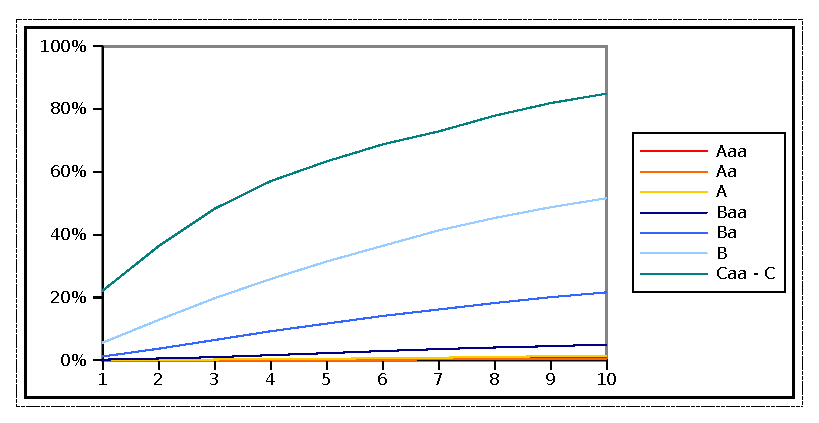
\includegraphics[bb=0 0 350 250]{probability_of_default.eps}
  \caption{Pravděpodobnost defaultu podle splatnosti a ratingového stupně (zdroj: Moody's)}
  \label{probability_of_default}
\end{figure}

Z grafu (\ref{probability_of_default}) je zřejmé, pravděpodobnost defaultu roste se zvyšující se zbytkovou splatností. Dále obecně platí, což vzhledem k měřítku není z grafu zcela patrné, že meziroční nárůst pravděpodobnosti defaultu je vyšší u vyšších ratingových skupin.

\subsection{Míra náhrady v případě defaultu}

Mírou náhrady rozumíme procentní část pohledávky, kterou získá věřitel zpět v případě, že dojde k defaultu společnosti. Za tímto účelem je vhodné rozdělit pohledávky do několika skupin dle pořadí, ve kterém jsou uspokojovány.

\subsubsection{Klasifikace pohledávek}

V případě, že dojde k defaultu, je z pohledu celkové ztráty, kterou utrpí věřitel, rozhodující tzv. seniorita dluhu. Seniorita dluhu určuje pořadí, ve kterém budou uspokojovány pohledávky jednotlivých věřitelů. Ti totiž nemusí mít při úhradě dluhu shodné postavení. Z tohoto pohledu je možné dluh rozdělit na seniorní a juniorní, kde seniorní dluh má přednost před juniorním.

Další velmi důležitou skutečností je zajištění dluhu. Je-li totiž dluh zajištěn určitým konkrétním majetkem, jako je např. nemovitost nebo pohledávka dlužníka vůči jinému subjektu, je nárok věřitele uspokojen z tohoto zajištění. To pohopitelně výrazně snižuje riziko ztráty.

Posledním dělením je rozlišení na standardní a podřízený dluh. Podřízený dluh stojí na pomezí mezi standardním dluhem a akciovým kapitálem. V případě finančních institucí je možné za přesně daných podmínek část podřízeného dluhu zahrnout do kapitálové přiměřenosti. Z logiky věci tedy vyplývá, že pohledávky z podřízeného dluhou jsou uspokojovány až po pohledávkách ze standardního dluhu.

\subsubsection{Míra náhrady v návaznosti na klasifikaci pohledávek}

Jak již bylo řečeno, je míra náhrady velmi ovlivněna tím, o jaký typ pohledávky se jedná. Následující tabulka shrnuje míru náhrady a její směrodatnou odchylku podle jednotlivých typů pohledávek.
\begin{center}
\begin{tabular}{c c c}
\textbf{Typ pohledávky} & \textbf{Míra náhrady} & \textbf{Směrodatná odchylka}\\
\hline
seniorní - zajištěná & 54\% & 27\% \\
seniorní - nezajištěná & 51\% & 25\% \\
seniorní - podřízená & 39\% & 24\% \\
podřízená & 33\% & 20\% \\
juniorní - podřízená & 17\% & 11\% \\
\end{tabular}
\end{center}
Z této tabulky je zřejmé, že z pohledu míry náhrady nehraje v případě standardní seniorní pohledávky zajištění výraznější roli. V případě podřízených pohledávek je pak rozhodující, je-li pohledávka seniorní nebo juniorní.

\section{Modelování kreditních spreadů}

Modely kreditního rizika lze rozdělit do dvou skupin a to na tzv. strukturované a redukované modely.

\subsection{Strukturované modely}

Strukturované modely jsou založené na tržní hodnotě společnosti. Vlastníci společnosti jsou chápáni jako majitelé opce, která jim umožňuje zdefaultovat v případě, že hodnota aktiv klesne pod hodnotu závazků. Tento typ modelu představili v první polovině 70.let Black a Scholes resp. Merton, kteří jej aplikovali na odvození ceny korporátního dluhopisu. Strukturované modely jsou založeny na předpokladu neexistence arbitráže, což umožňuje ignorovat očekávání a preference investorů.

\subsubsection{Mertonův model}

Merton ve svém modelu uvažuje společnost, kde tržní hodnota aktiv společnosti je podmíněna operativním rizikům a proto se náhodně mění. Kapitálová struktura uvažované společnosti je skládá pouze z akcií a diskontního dluhopisu.

Merton učinil dva předpoklady. Prvním předpokladem je, že společnost nemůže emitovat žádné cenné papíry, které by v porovnání s výše zmíněným diskontním dluhopisem byly seniornější. Druhým předpokladem je, že k defaultu nemůže dojít dříve než v době splatnosti diskontního dluhopisu. V době splatnosti dluhopisu tak mohou nastat dvě situace.
\begin{itemize}
\item Hodnota aktiv společnosti je dostatečná na to, aby došlo k úplnému splacení dluhopisu. Rozdíl mezi hodnotou aktiv a nominální hodnotou dluhopisu připadne akcionářům.
\item Hodnota aktiv společnosti není dostatečná na to, aby došlo k úplnému splacení dluhopisu. Akcionáři tak vzhledem ke své omezené majetkové zodpovědnosti vyhlásí default. Věřitelé se tak stávají majiteli veškerých aktiv společnosti.
\end{itemize}
Hodnota, která bude věřitelům v době splatnosti vyplacena je tak menší z celkové ceny aktiv a nominální hodnoty dluhopisu. To lze také chápat jako výplatu generovanou strategií, v rámci které nakoupíme bezrizikový diskontní dluhopis a prodáme prodejní opci na aktiva společnosti jejíž realizační cena se shoduje s nominální hodnotou dluhopisu. Akciový kapitál lze analogicky replikovat pomocí dlouhé pozice v kupní opci na aktiva společnosti jejíž realizační cena je rovna nominální hodnotě dluhopisu.\\

\noindent \textbf{Formální specifikace modelu} Jestliže je nominální hodnota dluhu splatného v čase $T$ rovna $F$ a hodnota aktiv v době splatnosti dluhu rovna $V$, je hodnota akciového kapitálu rovna
\begin{equation*}
E_T = \max(V_T - F, 0)
\end{equation*}
resp. hodnota dluhu z pohledu věřitelů rovna
\begin{equation*}
F - \max(F - V_T,0)
\end{equation*}

V Mertonově modelu je dynamika hodnoty společnosti modelována pomocí Brownova pohybu pro tzv. rizikově neutrální pravděpodobnostní míru jako
\begin{equation*}
d V_t = r V_t dt + \sigma_V V_t d W_t
\end{equation*}
kde $r$ je bezriziková úroková míra. Hodnota akciového kapitálu lze vypočíst pomocí Black-Scholes-Merton modelu pro oceňování kupní opce
\begin{equation}
E_t = V_t \Phi(d_1) - e^{-r(T-t)F \Phi(d_2)}
\end{equation}
kde
\begin{equation*}
d_1 = \frac{\ln \frac{V_t}{F} + \big(r + \frac{1}{2}\sigma_V^2\big)(T - t)}{\sigma_V \sqrt{T - t}}
\end{equation*}
\begin{equation*}
d_2 = d_1 - \sigma_V \sqrt{T - t}
\end{equation*}
a $\Phi(x)$ je pravděpodobnost, že náhodná veličina z normovaného normálního rozdělení je menší nebo rovna $x$. Hodnota dluhu je pak dána rovnicí
\begin{equation*}
D_t = V_t - E_t
\end{equation*}

\noindent \textbf{Implementace modelu} Hlavním problémem při aplikaci modelu je odhad tržní hodnoty aktiv a jejich volatility. V případě, že jsou na trhu kotovány ceny akcií a volatilita opcí na tyto akcie, je možné použít tyto kotace. Aplikací It\^o lemmy lze dokázat, že volatilita hodnoty aktiv se řídí vztahem
\begin{equation}
\sigma_E E_0 = \Phi(d_1)\sigma_V V_0
\end{equation}
Pro odhady $\sigma_E$ a $E_0$ lze na základě (13.1) a (13.2) odvodit $V_0$ a $\sigma_V$.\\

\noindent \textbf{Příklad:} Stanovme teoretickou hodnotu korporátního dluhopisu s nominální hodnotou 8 miliónů USD a splatností jeden rok emitovaného společností, jejíž hodnota aktiv $E_0$ je rovna 4 milióny USD a volatilita ceny akcií $\sigma_E$ je rovna 60\%. Předpokládejme, že bezriziková úroková sazba $r$ je 5\%.

Řešením rovnice
\begin{equation*}
E_0 = V_0 \Phi(d_1) - e^{-rT}F \Phi(d_2)
\end{equation*}
za podmínky
\begin{equation*}
\sigma_E E_0 = \Phi(d_1) \sigma_V V_0
\end{equation*}
získáme $V_0 = 11.59$ a $\sigma_V = 0.2108$. Hledanou hodnotu dluhu pak určíme jako $D_0 = V_0 - E_0$, tj. 11.59 - 4 = 7.59 miliónu USD. $\clubsuit$\\

\noindent \textbf{Časová struktura kreditních spreadů pro Mertonův model} Mertonův model může být kromě oceňování diskontních korporátních dluhopisů použit také pro odhad jejich kreditních spreadů.

Pro výnosovou míru diskontního dluhopisu $Y$ platí
\begin{equation*}
D_t = F e^{-Y^c(t,T)(T-t)}
\end{equation*}
Za předokladu konstantní bezrizikové úrokové míry $r$ je kreditní spread $S$ diskontního dluhopisu dán rovnicí
\begin{equation*}
S(t,T) \equiv Y^c(t,T) - r = \frac{1}{T-t}\ln \frac{F}{D_t} - r
\end{equation*}

Vztah mezi kreditním spreadem a splatností diskontního dluhopisu nazýváme časovou strukturou kreditních spreadů. Graf (\ref{credit_spread_1}) zobrazuje časovou strukturu kreditních spreadů společnosti z výše uvedeného příkladu.
\begin{figure}
  \centering
  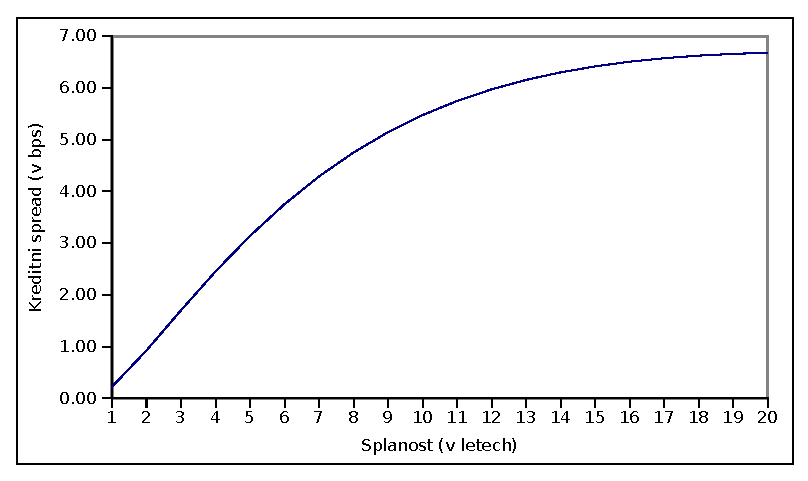
\includegraphics[bb=0 0 350 250]{credit_spread_1.eps}
  \caption{Rostoucí časová struktura kreditních spreadů}
  \label{credit_spread_1}
\end{figure}
Z grafu je zřejmé že kreditní spready rostou se splatností dluhopisu. Tento profil kreditních spreadů je typický pro situaci, kdy současná hodnota firmy převýší současnou hodnotu jejích závazků. V případě, že by vlastníci společnosti okamžitě splatili dluh, riziko defaultu by neexistovalo. Proto se s rostoucí splatností zvyšuje pravděpodobnost, že v době splatnosti nebude hodnota aktiv dostatečná na pokrytí dluhu.

Naopak, je-li současná hodnota závazků vyšší než současná hodnota společnosti, pak by svolání dluhu vedlo k defaultu společnosti. V tomto případě je časová struktura kreditních spreadů klesající. S rostoucí splatností se totiž zvyšuje pravděpodobnost, že v době splatnosti bude hodnota aktiv vyšší než hodnota závazků. Tuto situaci ilustruje graf (\ref{credit_spread_2}).
\begin{figure}
  \centering
  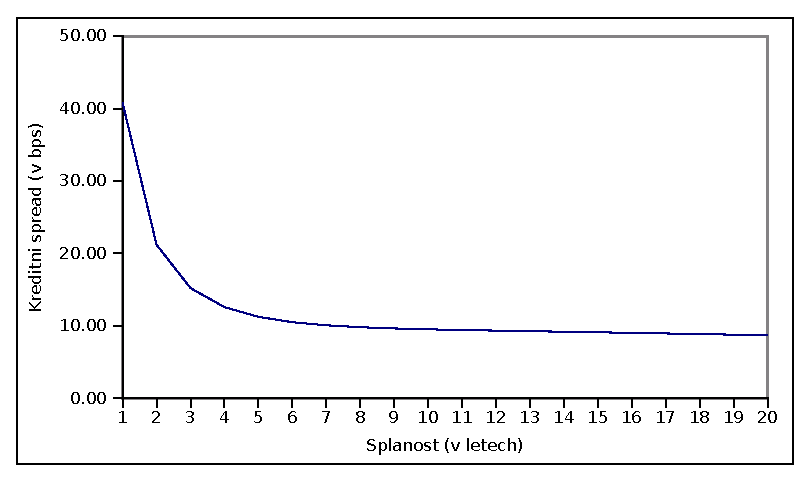
\includegraphics[bb=0 0 350 250]{credit_spread_2.eps}
  \caption{Klesající časová struktura kreditních spreadů}
  \label{credit_spread_2}
\end{figure}

Jestliže bychom rozděleli dluhopisy podle ratingového stupně a splatnosti a na základě jejich tržních kotací zkonstruovali časovou strukturu kreditních spreadů, získali bychom podobný profil jako v případě Mertonova modelu. Křivka kreditních spreadů by byla rostoucí v případě investičních ratingových skupin a klesající v případě spekulativních ratingových skupin. Také modely, které vznikly rozšířením původního Mertonova modelu, generují velmi podobný profil kreditních spreadů. To poukazuje na značnou robustnost tohoto modelu navzdory jeho zjednodušeným předpokladům a úzkému vymezení defaultu. 

\subsection{Rozšíření Mertonova modelu}

V roce 1979 rozšířil Geske Mertonův model o kupónové dluhopisy. Kupónové dluhopisy nelze v rámci Mertonova modelu chápat jako pouhý vážený součet diskontních dluhopisů. Neschopnost společnosti vyplatit kupón totiž implikuje default také na všechny následující platby generované dluhopisem. Geske proto chápal kupónový dluhopis jako složenou opci, kdy vlastníci společnosti mají možnost vyhlásit default při každé výplatě kupónu. Kupón tak bude vyplacen pouze v případě, že hodnota akciového kapitálu je po jeho výplatě vyšší než tento kupón.

Další rozšíření Mertonova modelu se zaměřilo na původní předpoklad, že k defaultu může dojít pouze v určitých předem známých časových okamžicích. V roce 1976 představil Black a Cox model, ve kterém má věřitel právo předčasně svolat diskontní dluhopis, jestliže hodnota aktiv společnosti klesne pod určitou exogenní hranici definovanou v úvěrové smlouvě. Věřitel tak může poslat společnost do konkurzu, jestliže hodnota aktiv klesne pod kritickou úroveň $h_t = h e^{-r(T-t)}$. Nedošlo-li k defaultu, obdrží věřitel v čase $T$ částku $\min(V_T,F)$. Došlo-li v čase $\tau$ k defaultu, obdrží věřitel částku $h_{\tau}$, kde $\tau$ je definováno jako $\tau \inf(t: V_t < h_t)$. Black a Cox odvodili explicitní rovnici pro oceňování diskontního dluhopisu a výpočet odpovídajícího kreditního spreadu\footnote{Postup odvození je následující. Uvědomme si, že věřitel získá $\min(V_T, D){\mathcal{I}_{(\tau \ge T)}} + h_{\tau}{\mathcal{I}_{(t < T)}}$, kde $\mathcal{I}_{(A)} = 1$ je-li A pravda a $\mathcal{I}_{(A)} = 0$ je-li A nepravda. První člen je přímo dán Mertonovým modelem a druhý člen může být oceněn stejným způsobem jako bariérová opce.}. Výsledná časová struktura kreditních spreadů je velmi podobná té, kterou získáme pomocí původního Mertonova modelu.

Black-Coxův model sloužil jako základ pro další navazující modely. Pravděpodobně nejznámnější je rozšíření, které v roce 1995 představili Longstaff a Schwartz. V jejich modelu úrokové sazby oscilují kolem určitého dluhodobého průměru (viz. např. Vašíčkův model úrokových sazeb) a nejsou korelovány se zdrojem nejistoty, kterým se řídí vývoj hodnoty aktiv společnosti. Model také připouští relativně složitou kapitálovu strukturu s odlišnou senioritou závazků. Longstaff a Schwarz definují default stejně jako v případě Black-Coxova modelu výhradně s ohledem na exogenní hranici. Tato podmínka umožnila konstrukci přímočarého modelu a také oceňování kupónových dluhopisů jako váženého součtu diskontních dluhopisů.

Navzdory jejich složitosti nejsou modely odvozené od původního Mertonova modelu výrazně lepším odrazem skutečnosti. To potvrdila také aplikace těchto modelů na reálných datech, kterou provedli např. Guoming, Wei a Guo (1997) nebo Eom a kol. (2002).

Společným znakem Mertonova modelu a modelů z něj odvozených je, že default lze do určité míry predikovat\footnote{Například tím, že se hodnota aktiv společnosti blíží hranici specifikované v úvěrové smlouvě.}. To předpokládá, že investoři mají k dispozici veškeré informace týkající finančního zdraví společnosti. Hodnata dluhopisů tak v případě defaultu postupně konverguje k míře náhrady. V praxi však hodnota dluhopisů vykazuje skoky, objeví-li se nová informace o zhoršené finanční situaci emitenta. To je v rozporu s předpokladem dokonalé informovanosti investorů. Reakcí na tuto skutečnost je snaha vytvořit modely, ve kterých by default nebyl predikovatelnou událostí. Tyto modely nazýváme redukovanými modely.

\subsection{Redukované modely}

V rámci redukovaného modelu má default společnosti charakter náhodné veličiny. Společnost tak nepředvidatelně zdefaultuje v náhodném časovém okamžiku. Pravděpodobnost defaultu v časovém okamžiku $t$ označme jako $p_t$. V případě konstantní okamžité pravděpodobnosti lze pravděpodobnost, že společnost nezdefaultuje v rámci malého časového intervalu $\Delta t$, vyjádřit jako $e^{-p \Delta t} \simeq 1 - p \Delta t$.

Uvažujme diskontní dluhopis, který v případě defaultu negeruje v době své splatnosti žádnou platbu. Předpokládejme, že dluhopis maturuje za $\Delta t$ roků. V době splatnosti tak tento diskontní dluhopis generuje platbu 1 USD s pravděpodobností $e^{-p \Delta t} \simeq 1 - p \Delta t$ popř. 0 USD s pravděpodobností $1 - e^{-p \Delta t} \simeq p \Delta t$. Cena tohoto dluhopisu v čase $t = 0$ je tak dána rovnicí
\begin{equation*}
P(0, \Delta t) = (e^{-p \Delta t} \times e^{-r \Delta t} \times 1) + \big( (1 - e^{-r \Delta t}) \times e^{-r \Delta t}\times 0 \big) = e^{-(r+p)\Delta t}
\end{equation*}
To znamená, že na rizikové dluhopisy lze aplikovat shodné oceňovací postupy jako na bezrizikové dluhopisy, pouze je třeba použít obecnou úrokou sazbu $\tilde{r} = r + p$.

Jestliže budeme uvažovat stochastické úrokové sazby a pravděpodobnost defaultu jako funkci času, pak lze současnou hodnotu diskontního dluhopisu se splatností v čase $T$ vyjádřit jako
\begin{equation*}
P(0,t) = E \Big[ e^{-\int_0^T (r_t + p_t)ds}\Big]
\end{equation*}
kde pro očekávanou hodnotu je použit ekvivalentní martingale (viz. příloha B kapitoly 12). Do výpočtu můžeme také zahnout míru náhrady. Jestliže $L_t$ vyjadřuje procentní výši ztráty věřitele v případě defaultu společnosti v čase $t$, je současná hodnota diskontního dluhopisu rovna
\begin{equation*}
P(0,T) = E \Big[ e^{-\int_0^T (r_t + p_t L_t)ds}\Big]
\end{equation*}

\subsubsection{Zjednodušený model}

V roce 1994 navrhl Fons zjednodušený model, který umožňuje investorům propojit ratingový stupeň s cenou dluhopisu. Model je založený na oceňování série cash-flow generovaného dluhopisem za předpokladu, že investoři jsou rizikově neutrální.

Uvažujme rizikový dluhopis s nominální hodnotou 1 USD, kupónem $C$, roční výplatou kupónů a splatností $T$ roků. Pravděpodobnost defaultu v roce $t$ za předpokladu, že dluhopis nezdefaultoval před rokem $t$, označme jako $p_t$. Pravděpodobnost, že dluhopis do roku $t$ nezdefaultuje je tak
\begin{equation*}
S_t = \prod_{s = 1}^t (1 - p_s)
\end{equation*}
Analogicky pravděpodobnost $D$, že dluhopis zdefaultuje v roce $t$ je rovna
\begin{equation*}
D_t = S_{t-1}p_t
\end{equation*}
Označme míru náhrady jako $\mu$. Očekávaná výše náhodného cash-flow $\tilde{F_t}$ obdrženého v čase $t$ je
\begin{equation*}
E[\tilde{F_t}] = S_tC + D_t \mu(1 + C)
\end{equation*}
Za předpokladu rizikově neutrálních investorů je cena dluhopisu v čase $t$ rovna
\begin{equation*}
P = \sum_t^T \frac{S_tC + D_t \mu(1 + C)}{(1 + r)^t} + \frac{S_T}{(1 + r)^T}
\end{equation*}
kde $r$ je výnos do splatnosti pro bezrizikového dluhopisu se shodnými charakteristikami. S pomocí ceny dluhopisu $P$ lze iteračně dopočíst spread $s$ z rovnice
\begin{equation}
P = \sum_{t=1}^T \frac{C}{(1 + r + s)^t} + \frac{1}{(1 + r + s)^T}
\end{equation}
V tomto pojetí modelu je investorům lhostejný důvod defaultu. Zajímají se pouze o jeho pravděpodobnost a míru náhrady. Očekávané pravděpodobnosti defaultu mohou být získány z historických údajů publikovaných ratingovými společnostmi. Každý cenný papír má tak na základě svého ratingu přiřazenu pravděpodobnost defaultu. Míra náhrady může být odhadnuta na základě seniority dluhopisu a legislativy, kterou se řídí příslušná emise.

Zásadním problémem výše popsaného modelu je předpoklad rizikově neutrálních investorů. Tento předpoklad však není v souladu s empirickou zkušeností. V důsledku této skutečnosti bychom ve Fonsově modelu měli namísto historické pravděpodobnosti defaultu použít rizikově upravenou pravděpodobnost defaultu. Této problematice se věnuje následující podkapitola.

\subsection{Historická a rizikově upravená pravděpodobnost defaultu}

Na základě ceny dluhopisu a odhadnuté míry náhrady je možné odvodit implikovanou pravděpodobnost defaultu. Uvažujme rovnici (13.3) ve zjednodušené formě s konstantními parametry. Spread nad bezrizikovou sazbou lze vypočíst jako $s = pL = p(1 - R)$, kde $p$ je pravděpodobnost defaultu, $L$ je procentní výše ztráty v případě defaultu a $R$ je míra náhrady. Typický dluhopis s ratingem A emitovaný ve Spojených státech má oproti srovnatelnému dluhopisu typicky spread 50 bps. Předpokládejme míru náhrady 10\%. Implikovaná pravděpodobnost defaultu je pak rovna 0.56\%.
\begin{equation*}
p = \frac{s}{1 - R} = \frac{0.005}{1 - 0.1} = 0.005556
\end{equation*} 
Podle přechodové matice je historická pravděpodobnost defaultu společnosti s ratingem A v průběhu jednoho roku 0.05\%. To je, i při extrémně nízké použité míře náhrady, desetkrát méně než výše vypočtená implikovaná pravděpodobnost defaultu. Implikovaná pravděpodobnost defaultu vychází v porovnání s historickou pravděpodobností defaultu systematicky výrazně vyšší. Tento jev lze vysvětlit pomocí likviditní přirážky popř. pomocí katastrofických scénářů, které investoři promítají do ceny dluhopisu a které jsou sice teoreticky možné, avšak v minulosti nenastaly. Formální vysvětlení je takové, že pravděpodobnost defaultu odhadnutá na základě ceny dluhopisu je rizikově neutrální, kdežto historická pravděpodobnost defaultu se opírá o reálný svět.

V Mertonově modelu je použita historická pravděpodobnost defaultu $p$, která vyjadřuje pravděpodobnost, že hodnota aktiv společnost klesne pod nominální hodnotu diskontního dluhopisu.
\begin{equation*}
p = P[V_T < F]
\end{equation*}
Předpokládejme, že hodnota aktiv sleduje Brownův pohyb
\begin{equation*}
\frac{d V_t}{V_t} = \mu_v dt + \sigma_V d W_t^V
\end{equation*}
Aplikací It\^o lemmy a integrováním od $t$ do $T$ získáme
\begin{equation}
p_{t,T} = \Phi \Big( \frac{\ln F - \ln V_0 - \mu_v(T-t) + \frac{1}{2}\sigma_V^2(T-t)}{\sigma_V \sqrt{T-t}}\Big)
\end{equation}
kde $p_{t,T}$ vyjadřuje pravděpodobnost v čase $t$, že společnost zdefaultuje do časového okamžiku $T > t$, a $\Phi(x)$ je funkce kumulativního normovaného normálního rozdělení.

Rovnice pro rizikově neutrální pravděpodobnost je podobná (13.4) se tím rozdílem, že $\mu_V$ je nahrazeno bezrizikovou úrokovou mírou $r$. S využitím Sharpeho modelu CAPM lze zformulat vztah mezi očekávanou výnosovou mírou na aktiva společnosti a očekávanou výnosovou mírou tržního portfolia jako
\begin{equation*}
\mu_V - r = \frac{cov(\mu_V, \mu_M)}{\sigma_M^2}(\mu_M - r) = \sigma_V \rho_{M,V} \beta
\end{equation*}
kde $\beta = \frac{\mu_V - r}{\sigma_M}$ lze interpretovat jako tržní cenu rizika. Připomeňme, že pro rizikově neutrální pravděpodobnost defaultu nahradí bezriziková úroková míra $r$ ve vzorci pro historickou pravděpodobnost defaultu očekávanou výnosovou míru na aktiva společnosti $\mu_V$. Rizikově neurální pravděpodobnost defaultu $q_{t,T}$ pak lze na základě (13.4) vyjádřit jako
\begin{equation*}
q_{t,T} = \Phi \big( \Phi^{-1}(p_{t,T}) + \rho_{M,V}\beta \sqrt{T-t})\Big)
\end{equation*}
Takto formulovaná rizikově neutrální pravděpodobnost defaultu je založena na předpokladu, že k defaultu společnosti může dojít pouze v době splatnosti diskontního dluhopisu. Výše uvedenou analýzu však lze relativně snadno modifikovat tak, aby bylo možné vypočíst rizikově neutrální pravděpodobnost defaultu za předpokladu, že se společnost po protnutí hranice defaultu nezotaví. Bohn (1999) prokázal, že pro aproximaci prvního řádu, tento předpoklad znamená pouze malou úpravu původní rovnice na
\begin{equation*}
q_{t,T} = 2\Phi \Big( \Phi^{-1}\Big(\frac{1}{2}p_{t,T}\Big) + \rho_{M,V}\beta \sqrt{T-t})\Big)
\end{equation*}
Všimněme si, že pokud $\rho_{M,V} = 0$ platí $p(t,T) = q(t,T)$. Je-li $\rho_{M,V} > 0$, tj. parametr $\beta$ dané společnosti je kladný, je rizikově neutrální pravděpodobnost defaultu vyšší než historická pravděpodobnost defaultu. Pokud dojde k poklesu hodnoty aktiv společnosti, okamžitá pravděpodobnost defaultu roste. To se pro $\beta > 0$ stane v průměru vždy, když klesne hodnota tržního portfolia. Riziko defaultu není diverzikovatelné a k defaultu dochází častěji v případech, když je trh na sestupu. Proto je cena rizika vyšší a rizikově neutrální pravděpodobnost defaultu je tak vyšší než historická pravděpodobnost defaultu.

\part{Plain-vanilla opce a exotické deriváty}

\chapter{Dluhopisy s vnořenou opcí a opce na dluhopisy}

\section{Svolatelný dluhopis a dluhopis s právem zpětného prodeje}

Svolatelný dluhopis resp. dluhopis s právem zpětného odkupu obsahují vnořenou kupní resp. prodejní opci. Ta může být, v závislosti smluvních podmínkách, uplatněna od určitého data popř. pouze k určitému datu resp. datům.

\subsection{Charakteristika}

Svolatelný dluhopis může být emitentem zpětně odkoupen před datem své splatnosti za předem dohodnutou cenu. Z pohledu investora jej tedy lze replikovat pomocí dlouhé pozice v plain-vanilla dluhopisu a krátké pozice v kupní opci na tento dluhopis. Jestliže dojde k poklesu úrokových sazeb, umožňuje emitentovi vnořená opce dluhopis odkoupit za fixní cenu a emitovat nový dluhopis za výhodnějších podmínek. Z pohledu investora má svolatelný dluhopis dvě nevýhody. První nevýhodou je, že v případě svolání dluhopisu emitentem je investor nucen reinvestovat při nižší výnosové míře. Druhou související nevýhodou je, že při poklesu úrokových sazeb je růst ceny svolatelného dluhopisu nižší než růst ceny obdobného plain-vanilla dluhopisu. Této vlastnosti říkáme negativní konvexita. Je zřejmé, že vzhledem k výhodám na straně emitenta, musí být cena svolatelného dluhopisu v porovnání se standardním dluhopisem nižší. 

Dluhopis s právem zpětného prodeje může být před svou splatností prodán emitentovi za předem dohodnutou cenu a lze jej tedy replikovat pomocí dlouhé pozice v plain-vanilla dluhopisu a v prodejní opci na tento dluhopis. Dluhopis s právem zpětného prodeje umožňuje investorovi jej v případě růstu úrokových sazeb prodat emitentovi za předem dohodnutou cenu a nakoupit dluhopis s vyšší výnosovou mírou. Z logiky věci je tedy zřejmé, že cena tohoto dluhopisu v porovnání s obdobným plain-vanilla dluhopisem vyšší.

\subsection{Oceňování}

Cash-flow generované svolatelným dluhopisem a dluhopisem s právem zpětného prodeje nejsou dopředu známé. Pro oceňování těchto dluhopisů je tak třeba použít binomický strom popř. metodu Monte Carlo.

\subsubsection{Yield-to-worst metoda}

Před tím, že se budeme zabývat oceňováním pomocí binomického stromu a metody Monte Carlo, představme si tradiční metodu yield-to-worst. Spíše než o oceňovací metodu se jedná o přístup, který umožňuje učinit si představu o riziku potenciální výnosové míry spojeného se svolatelným dluhopisem.

Uvažujme svolatelný dluhopis, který může je obchodován nad par. Vedle klasického výnosu do splatnosti vypočteme také výnosy k datům, ve kterých může být dluhopis svolán emitentem. Yield-to-worst je pak nejnižší z těchto výnosových měr.\\

\noindent \textbf{Příklad:} Ohodnoťme potenciální výnos, který můžeme získat na desetiletý dluhopis s roční kupónovou sazbou 5\%. Předpokládejme, že dluhopis může být svolán počínaje pátým rokem vždy na konci roku. Dále předpokládejme, že dluhopis je aktuálně obchodován za cenu 102.

Pro pátý až devátý rok, kdy může být dluhopis svolán emitentem, vypočtěme výnos do svolání. Pro desátý rok vypočteme výnos do splatnosti. Výsledky shrnuje níže uvedená tabulka.
\begin{center}
\begin{tabular}{c c}
\textbf{Rok} & \textbf{Splatnost (\%)} \\
\hline
5  & 4.54 \\
6  & 4.61 \\
7  & 4.66 \\
8  & 4.69 \\
9  & 4.72 \\
10 & 4.74 \\
\end{tabular}
\end{center}
Yield-to-worst tohoto dluhopisu je tedy 4.54\%. $\clubsuit$\\

Yield-to-worst je tedy nejnižší výnos generovaný svolatelným dluhopisem, kterého investor dosáhne pro aktuální tržní cenu. V případě dluhopisu s právem zpětného prodeje, postrádá yield-to-worst smysl, protože o zpětném odkupu rozhoduje investor. Stejně jako výnos do splatnosti je yield-to-worst založen na následujících předpokladech.
\begin{itemize}
\item Investor drží svolatený dluhopis až do data jeho svolání resp. splatnosti.
\item Kupónové platby generované dluhopisem jsou reinvestovány za výnos rovný yield-to-worst.
\end{itemize}
Tento přístup tak nebere v potaz cenové riziko (prodej dluhopisu před jeho svoláním resp. splatností) ani reinvestiční riziko.

\subsubsection{Oceňování dluhopisu pomocí spotových a forwardových úrokových sazeb}

S ohledem na značně zjednodušený přístup nelze yield-to-worst považovat za přijatelně přesnou metodu oceňování svolatelných dluhopisů. Pro tento účel je třeba zohlednit náhodnost budoucích úrokových sazeb. Modely pro oceňování svolatelných dluhopisů a dluhopoisů s právem zpětného prodeje mají následující vlastnosti.
\begin{itemize}
\item Předpokládá se, že úrokové sazby se řídí lognormálním rozdělením. To má za následek, že změny úrokových sazeb jsou proporcionální k úrovni úrokových sazeb a že úrokové sazby nemohou být negativní.
\item Modely jsou zkonstruovány tak, aby neumožňovaly arbitráž. Musí tedy zcela reflektovat aktuální ceny plain-vanilla bezrizikových dluhopisů.
\end{itemize}
Pro pochopení následující kapitoly je třeba si uvědomit, že dluhopis je možné oceňovat pomocí spotových a forwardových úrokových sazeb, přičemž výsledná cena je v případě obou přístupů stejná. Pro ilustraci uveďme příklad.\\

\noindent \textbf{Příklad:} Uvažujme dluhopis s tříletou zbytkovou splatností a roční kupónovou sazbou 5\% a nominální hodnotou 100 USD. Označme aktuální zero sazbu se splatností $t$ roků jako $R(0,t)$ a aktuální forwardovou sazbu pro časovou periodu $s$ až $t-s$, kde $t > s$ jako $F(0,s,t-s)$. Současná cena dluhopisu je
\begin{equation*}
P = \frac{5}{1 + R(0,1)} + \frac{5}{\big(1 + R(0,2)\big)^2} + \frac{105}{\big( 1 + R(0,3)\big)^3}
\end{equation*}
popř. alternativně
\begin{gather*}
P = \frac{5}{1 + R(0,1)} + \frac{5}{\big( 1 + R(0,1)\big)\big( 1 + F(0,1,1)\big)} + \\
 + \frac{105}{\big( 1 + R(0,1)\big)\big( 1 + F(0,1,1)\big)\big( 1 + F(0,2,1)\big)} = \frac{\frac{\frac{105}{1 + F(0,2,1)} + 5}{1 + F(0,1,)} + 5}{1 + R(0,1)}
\end{gather*}
Z konečného tvaru druhé rovnice je patrné, že na oceňování dluhopisu je možné pohlížet jako na rekurzivní proces. Na konci třetího roku v době své splatnosti má dluhopis hodnotu 105 USD. Hodnotu dluhopisu na konci druhého roku určíme jako hodnotu dluhopisu na konci třetího roku diskontnovanou forwardovou sazbou pro časové období dva až tři roky. Hodnotu dluhopisu na konci prvního roku určíme jako hodnotu dluhopisu na konci druhého roku navýšenou o kupónovou platbu 5 USD diskontovanou forwardovou sazbou pro časové období jeden až dva roky. Současnou hodnotu dluhopisu pak určíme jako hodnotu dluhopisu na konci prvního roku navýšenou o kupónovou platbu 5 USD diskontovanou spotovou zero sazbou se splatností jeden rok. $\clubsuit$\\

Přístup, který jsme popsali ve výše uvedeném příkladě, je klíčový pro oceňování svolatelných dluhopisů a dluhopisů s právem zpětného prodeje. Jediný rozdíl spočívá v tom, že namísto forwardových úrokových sazeb budou použity modelované budoucí krátkodobé úrokové sazby.

\subsubsection{Oceňování pomocí binomického stromu}

Uvažujme binomický strom úrokových sazeb. Tento binomický strom použijeme k rekurzivnímu ocenění dluhopisů s vnořenou opcí. Dále uvažujme svolatelný dluhopis, jehož nominální hodnota $V$ je splatná na konci životnosti $T$ s roční kupónovou sazbou $C$. Předpokládejme, že data svolání jsou $T_k$ a jim odpovídající cena, za kterou emitent odkoupí dluhopis, je rovna $CP_k$.
\begin{center}
\begin{pspicture}(0,0)(12,6.5)
     \rput(6.0,0.0){Oceňování svolatelného dluhopisu pomocí binomického stromu}

	\psline(1.0,3.5)(3.0,4.0)
	\psline(1.0,3.5)(3.0,3.0)
	
	\psline(3.0,4.0)(5.0,4.5)
	\psline(3.0,4.0)(5.0,3.5)
	\psline(3.0,3.0)(5.0,3.5)
	\psline(3.0,3.0)(5.0,2.5)

     \psline(7.0,4.5)(9.0,5.0)
     \psline(7.0,4.5)(9.0,4.0)
     \psline(7.0,3.5)(9.0,4.0)
     \psline(7.0,3.5)(9.0,3.0)
     \psline(7.0,2.5)(9.0,3.0)
     \psline(7.0,2.5)(9.0,2.0)
     
     \psline(9.0,5.0)(11.0,5.5)
     \psline(9.0,5.0)(11.0,4.5)
     \psline(9.0,4.0)(11.0,4.5)
     \psline(9.0,4.0)(11.0,3.5)
     \psline(9.0,3.0)(11.0,3.5)
     \psline(9.0,3.0)(11.0,2.5)
     \psline(9.0,2.0)(11.0,2.5)
     \psline(9.0,2.0)(11.0,1.5)

     \rput(0.7,3.5){\tiny{$P$}}
     \rput(3.0,4.3){\tiny{$P_u$}}
     \rput(3.0,3.3){\tiny{$P_l$}}
     \rput(5.3,4.5){\tiny{$P_{2u}$}}
     \rput(5.3,3.5){\tiny{$P_{u,l}$}}
     \rput(5.3,2.5){\tiny{$P_{2l}$}}
     \rput(6.5,4.5){\tiny{$P_{(n-1)u}$}}
     \rput(6.3,3.5){\tiny{$P_{(n-k)u,kl}$}}
     \rput(6.3,2.5){\tiny{$P_{(n-1)l}$}}
     \rput(9.0,5.2){\tiny{$P_{nu}$}}
     \rput(9.0,4.3){\tiny{$P_{(n-1)u,l}$}}
     \rput(9.0,3.3){\tiny{$P_{(n-x)u,xl}$}}
     \rput(9.0,2.3){\tiny{$P_{(n-1)l}$}}
     \rput(11.5,5.5){\tiny{$V + C$}}
     \rput(11.5,4.5){\tiny{$V + C$}}
     \rput(11.5,3.5){\tiny{$V + C$}}
     \rput(11.5,2.5){\tiny{$V + C$}}
     \rput(11.5,1.5){\tiny{$V + C$}}
     
     \psline[linestyle=dotted](1.0,3.5)(1.0,1.0)
     \psline[linestyle=dotted](3.0,3.0)(3.0,1.0)
     \psline[linestyle=dotted](5.0,2.5)(5.0,1.0)
     \psline[linestyle=dotted](7.0,2.5)(7.0,1.0)
     \psline[linestyle=dotted](9.0,2.0)(9.0,1.0)
     \psline[linestyle=dotted](11.0,1.5)(11.0,1.0)
     
     \rput(1.0,0.7){\tiny{0}}
     \rput(3.0,0.7){\tiny{1}}
     \rput(5.0,0.7){\tiny{2}}
     \rput(7.0,0.7){\tiny{$n-1$}}
     \rput(9.0,0.7){\tiny{$n$}}
     \rput(11.0,0.7){\tiny{splatnost}}
\end{pspicture}
\end{center}
Pro cenu na začátku $n$-té periody platí
\begin{equation*}
P_{nu} = \frac{V + C}{1 + r_{nu}}
\end{equation*}
resp. obecně
\begin{equation*}
P_{(n-k)u, kl} = \frac{V + C}{1 + r_{(n-k)u,kl}}
\end{equation*}
Analogicky cenu svolatelného dluhopisu na začátku periody $n-1$ lze vypočíst jako
\begin{equation*}
P_{(n-1)u} = \frac{1}{2}\Bigg( \frac{\min(P_{nu}, CP_{n}) + C}{1 + r_{(n-1)u}} + \frac{\min(P_{(n-1)u,l}, CP_{n}) + C}{1 + r_{(n-1)u}}\Bigg)
\end{equation*}
resp. obecně jako
\begin{equation*}
P_{(n-1-k)u, kl} = \frac{1}{2}\Bigg( \frac{\min(P_{(n-k)u,kl}, CP_{n}) + C}{1 + r_{(n-1-k)u,kl}} + \frac{\min(P_{(n-1-k)u,kl}, CP_{n}) + C}{1 + r_{(n-1-k)u,kl}}\Bigg)
\end{equation*}
Cash-flow, které v periodě $n-1$ diskontujeme, je menší z ceny dluhopisu vypočtené pro $n$-tou periodu a ceny, za kterou je možné dluhopis svolat. Podobný způsobem postupujeme až k vrcholu binomického stromu, kde pro začátek první periody získáme
\begin{equation*}
P_u = \frac{1}{2} \Bigg( \frac{\min(P_{uu}, CP_2)+C}{1 + r_u} + \frac{\min(P_{ul}, CP_2) + C}{1 + r_u} \Bigg)
\end{equation*}
resp.
\begin{equation*}
P_l = \frac{1}{2} \Bigg( \frac{\min(P_{ul}, CP_2)+C}{1 + r_l} + \frac{\min(P_{ll}, CP_2) + C}{1 + r_l} \Bigg)
\end{equation*}
Hodnota svolatelného dluhopisu na začátku nulté periody, tj. v současná hodnota dluhopisu, je tak rovna
\begin{equation*}
P = \frac{1}{2}\Bigg( \frac{\min(P_u, CP_1) + C}{1 + y_t} + \frac{\min(P_l, CP_1) + C}{1 + y_t}\Bigg)
\end{equation*}
V případě dluhopisu s právem zpětného prodeje je postup výpočtu shodný s tím rozdílem, že v každém uzlu budeme namísto minima z ceny dluhopisu a ceny a realizační ceny vnořené opce aplikovat maximum.\\

\noindent \textbf{Příklad:} Uvažujme níže uvedený binomický strom úrokových sazeb, kde pravděpodobnost růstu úrokové sazby a pravděpodobnost poklesu úrokové sazby je v každém uzlu rovna 50.00\%. 
\begin{center}
  \begin{pspicture}(0,0)(10.5,7.0)

	\psline[linewidth=0.5mm](1.0,3.5)(3.0,4.0)
	\psline[linewidth=0.5mm](1.0,3.5)(3.0,3.0)

	\psline[linewidth=0.5mm](3.0,4.0)(5.0,4.5)
	\psline[linewidth=0.5mm](3.0,4.0)(5.0,3.5)
	\psline[linewidth=0.5mm](3.0,3.0)(5.0,3.5)
	\psline[linewidth=0.5mm](3.0,3.0)(5.0,2.5)

	\psline[linewidth=0.5mm](5.0,4.5)(7.0,5.0)
	\psline[linewidth=0.5mm](5.0,4.5)(7.0,4.0)
	\psline[linewidth=0.5mm](5.0,3.5)(7.0,4.0)
	\psline[linewidth=0.5mm](5.0,3.5)(7.0,3.0)
	\psline[linewidth=0.5mm](5.0,2.5)(7.0,3.0)
	\psline[linewidth=0.5mm](5.0,2.5)(7.0,2.0)

	\psline[linewidth=0.5mm](7.0,5.0)(9.0,5.5)
	\psline[linewidth=0.5mm](7.0,5.0)(9.0,4.5)
	\psline[linewidth=0.5mm](7.0,4.0)(9.0,4.5)
	\psline[linewidth=0.5mm](7.0,4.0)(9.0,3.5)
	\psline[linewidth=0.5mm](7.0,3.0)(9.0,3.5)
	\psline[linewidth=0.5mm](7.0,3.0)(9.0,2.5)
	\psline[linewidth=0.5mm](7.0,2.0)(9.0,2.5)
	\psline[linewidth=0.5mm](7.0,2.0)(9.0,1.5)

	\rput(0.4,3.5){\tiny{1.65000}}

	\rput(2.7,4.3){\tiny{2.47609}}
	\rput(3.0,3.3){\tiny{2.42706}}

	\rput(4.7,4.8){\tiny{3.62889}}
	\rput(5.0,3.8){\tiny{3.55704}}	
	\rput(5.0,2.8){\tiny{3.48660}}

	\rput(6.7,5.3){\tiny{4.20215}}
	\rput(7.0,4.3){\tiny{4.11894}}	
	\rput(7.0,3.3){\tiny{4.03738}}
	\rput(7.0,2.3){\tiny{3.95743}}

	\rput(9.6,5.5){\tiny{4.51393}}
	\rput(9.6,4.5){\tiny{4.42454}}	
	\rput(9.6,3.5){\tiny{4.33693}}
	\rput(9.6,2.5){\tiny{4.25106}}
	\rput(9.6,1.5){\tiny{4.16688}}

	\psline[linestyle=dotted](1.0,3.5)(1.0,1.0)
	\psline[linestyle=dotted](3.0,3.0)(3.0,1.0)
	\psline[linestyle=dotted](5.0,2.5)(5.0,1.0)
	\psline[linestyle=dotted](7.0,2.0)(7.0,1.0)
	\psline[linestyle=dotted](9.0,1.5)(9.0,1.0)

	\rput(1.0,0.7){\tiny{1}}
	\rput(3.0,0.7){\tiny{2}}
	\rput(5.0,0.7){\tiny{3}}
	\rput(7.0,0.7){\tiny{4}}
	\rput(9.0,0.7){\tiny{5}}

  \end{pspicture}
\end{center}
Dále uvažujme dluhopis s nominální hodnotou 100 USD, s ročním kupónem 2 USD a se zbytkovou splatností tři roky, který je svolatelný za par vždy na konci roku. V souladu s výše uvedeným postupem lze cenu svolatelného dluhopisu vypočíst jako
\begin{equation*}
\frac{1}{2}\frac{\frac{1}{2}\min \Bigg(\frac{\frac{1}{2}\min \Big( \frac{100 + 2}{1.0362889},100 \Big) + \frac{1}{2}\min \Big( \frac{100 + 2}{1.0355704},100 \Big) + 2}{1.0247609},100 \Bigg)}{1.01650} +
\end{equation*}
\begin{equation*}
+  \frac{1}{2}\frac{\frac{1}{2}\min \Bigg(\frac{\frac{1}{2}\min \Big( \frac{100 + 2}{1.0355704},100 \Big) + \frac{1}{2}\min \Big( \frac{100 + 2}{1.0348660},100 \Big) + 2}{1.0242706},100 \Bigg)}{1.01650} + \frac{2}{1.01650} = 98.46666
\end{equation*}
Hodnota uvažovaného svolatelného dluhopisu je tedy rovna 98.46666. Pro porovnání hodnota ekvivalentního plain-vanilla dluhopisu je rovna 99.90228.
$\clubsuit$\\

V praxi naráží výše uvedený postup oceňování svolatelného dluhopisu resp. dluhopisu s právem zpětného prodeje na řadu problémů.
\begin{itemize}
\item Vzhledem k tomu, že řada dluhopisů generuje kupónovou platbu poleletně popř. čtvrtletně, musí být časový krok při konstrukci úrokového stromu kratší než jeden rok. Kratší časový krok na jedné straně zpřesňuje ocenění, což se projeví zejména u krátkodobých dluhopisů, na druhé straně však poměrně výrazně zesložiťuje výpočet.
\item V řadě případů má vnořená opce charakter americké opce, která může být uplatněna kdykoliv v průběhu životnosti dluhopisu. Tato skutečnost vyžaduje velmi krátký časový krok při konstrukci binomického stromu úrokových sazeb. Složitost ocenění však roste exponenciálně s počtem časových kroků, které vstupují do výpočtu.
\item Velmi často se stává, že cash-flow generované dluhopisem nekoresponduje s časovou strukturou binomického stromu úrokových sazeb. To pochopitelně komplikuje implementaci modelu.
\item Problematická je také volatilita krátkodobé úrokové sazby, která představuje klíčový vstup modelu. Lze použít historickou volatilitu popř. volatilitu, kterou implikují ceny úrokových opcí kotované na trhu. V rámci modelu také předpokládáme fixní volatilitu pro všechny splatnosti, což je velmi zjednodušující předpoklad.
\end{itemize}

\subsubsection{Metoda Monte-Carlo}

Současnou krátkodobou úrokovou sazbu označme jako $r$. Předpokládejme, že dynamika úrokové sazby se řídí rovnicí
\begin{equation*}
\Delta r_t = r_{t + \Delta t} - r_t = \mu(r,t)\Delta t + \sigma(r,t) \varepsilon \sqrt{\Delta t}
\end{equation*}
kde $\Delta t$ je délkou časového kroku, $\Delta r$ představuje změnu úrokové sazby v průběhu jednoho časového kroku, $\mu {r ,t}$ vyjadřuje očekávanou změnu úrokové sazby v průběhu jednoho časového kroku, $\sigma(r,t)$ je směrodatná odchylka krátkodobé úrokové sazby v průběhu jednoho časového kroku a $\varepsilon$ je náhodná veličina z normovaného normálního rozdělení.

Nechť pro zjednodušení platí
\begin{gather*}
\mu(r,t) = \mu r \\
\sigma(r,t) = \sigma r
\end{gather*}
kde $\mu$ a $\sigma$ jsou konstanty. Platí tedy
\begin{equation*}
\Delta r = \mu r \Delta t + \sigma r \varepsilon \sqrt{\Delta t}
\end{equation*}
Pro účely ocenění je třeba vygenerovat trajektorie úrokových sazeb.\\

\noindent \textbf{Příklad:} Předpokládejme, že aktuální jednoletá úroková sazba je rovna 4.00\%. Předpokládejme, že $\mu = 0.045$ a $\sigma = 0.05$ pro časový interval jednoho roku. Dále předpokládejme, že délka časového kroku je jeden rok. Meziroční změna úrokové sazby je tak dána rovnicí
\begin{equation*}
\Delta r = 0.045 r + 0.05 r \varepsilon
\end{equation*}
Označme jednoletou úrokovou sazbu v roce $k$ jako $r_k$. Pak platí
\begin{gather*}
r_0 = 0.04 \\
r_k = 0.045 r_{k-1} + 0.05 r_{k-1} \varepsilon
\end{gather*}
Následující tabulka představuje šest trajektorií úrokových sazeb generovaných se splatností deset let.
\begin{center}
\begin{tabular}{c c c c c c c}
\multirow{2}{*}{\textbf{Rok}} & \multicolumn{6}{c}{\textbf{Trajektorie}} \\
 & \textbf{1} & \textbf{2} & \textbf{3} & \textbf{4} & \textbf{5} & \textbf{6} \\
\hline
1  & 4.00 & 4.00 & 4.00 & 4.00 & 4.00 & 4.00 \\
2  & 4.08 & 4.14 & 4.29 & 4.24 & 4.28 & 4.28 \\
3  & 3.83 & 4.02 & 4.35 & 4.27 & 4.24 & 4.23 \\
4  & 4.15 & 3.88 & 4.25 & 3.87 & 4.17 & 4.30 \\
5  & 4.27 & 4.26 & 4.68 & 4.58 & 4.29 & 3.99 \\
6  & 4.69 & 4.49 & 4.33 & 4.29 & 4.47 & 4.32 \\
7  & 4.88 & 5.10 & 5.24 & 5.08 & 5.27 & 4.70 \\
8  & 5.14 & 4.94 & 4.75 & 5.54 & 5.25 & 5.08 \\
9  & 5.24 & 5.47 & 5.15 & 5.26 & 5.43 & 5.64 \\
10 & 5.59 & 5.04 & 5.29 & 5.58 & 5.38 & 5.02 \\
\end{tabular}
\end{center}
$\clubsuit$\\

V praxi je model kalibrován na aktuální výnosovou křivku pomocí členu $\mu(r,t) \Delta t$ tak, aby teoretická cena kupónového par dluhopisu byla rovna 100.

V dalším kroce je třeba rekurzivně vypočíst hodnotu dluhopisu pro každou z trajektorií. Uvažujme svolatelný dluhopis se splatností $n$ let, kde $n > 5$, ročním kupónem ve výši $C$, nominální hodnotou $V$ a cenou, za kterou je možné dluhopis na konci roku svolat, rovnou $CP$. Nechť $P_k$ je cena dluhopisu v roce $k$ a $r_k$ je jednoletá úroková sazba pro $k$-tý rok. Platí
\begin{gather*}
P_{n-1} = \frac{V + C}{1 + r_{n-1}} \\
P_{n-2} = \frac{\min(P_{n-1},CP) + C}{1 + r_{n-2}} \\
\dots \\
P_4 = \frac{\min(P_5,CP) + C}{1 + r_4} \\
P_3 = \frac{\min(P_4,CP) + C}{1 + r_3} \\
\dots \\
P_0 = \frac{P_1 + C}{1 + r_0}
\end{gather*}
\noindent \textbf{Příklady:} Uvažujme svolatelný dluhopis s nominální hodnotou 100 USD a roční kupónovou platbou 4.75 USD, zbytkovou splatností 10 let. Předpokládejme, že dluhopis může být svolán po 5 letech vždy na konci roku za cenu 100 USD. Cenu tohoto dluhopisu pro trajektorie úrokových sazeb odvozených v předchozím příkladě shrnuje následující tabulka.
\begin{center}
\begin{tabular}{c c c c c c c}
 & \multicolumn{6}{c}{\textbf{Trajektorie}} \\
 & \textbf{1} & \textbf{2} & \textbf{3} & \textbf{4} & \textbf{5} & \textbf{6} \\
\hline
\textbf{Cena}  & 100.43 & 100.55 & 99.90 & 99.76 & 99.68 & 100.55
\end{tabular}
\end{center}
$\clubsuit$\\

Posledním krokem je výpočet průměrné ceny svolatelného dluhopisu na základě cen pro jednotlivé trajektorie.\\

\noindent \textbf{Příklad:} Výsledná cena svolatelného dluhopisu uvažovaného v předchozím příkladě je tedy rovna 100.14 USD.
\begin{equation*}
P = \frac{1}{6}(100.43 + 100.55 + 99.90 + 99.76 + 99.68 + 100.55) = 100.14
\end{equation*}
$\clubsuit$\\

V našem ilustračním příkladě jsme použili pouze šest trajektorií úrokových sazeb. Mezi počtem trajektorií a přesností výpočtu však existuje přímá úměrnost. V praxi je třeba použít alespoň 500 trajektorií, jestliže chceme dosáhnout dostatečně přesného výsledku.

\subsection{OAS spread}

Cenu dluhopisu lze alternativně vyjádřit pomocí spreadu. Ten vyjadřuje, o kolik bazických bodů je třeba posunout referenční výnosovou křivku, aby se teoretická cena dluhopisu rovnala ceně kotované trhem. V případě dluhopisů s vnořenou opcí se pro tyto účely využívá tzv. OAS (option-adjusted) spread. OAS spread zohledňuje skutečnost, že s posunem výnosové křivky dochází nejen ke změně diskontních faktorů ale také ke změně ceny vnořené opce. Tento spread zavisí na volatilitě krátkodobých sazeb. V případě svolatelného dluhopisu znamená vysoká volatilita nižší teoretickou cenu dluhopisu a tím pádem vyšší OAS spread. V případě dluhopisu s přednostním právem prodeje je tomu naopak. Vzhledem k tomu, že se ve většině případů jako referenční výnosová křivka používá výnosová křivka státních dluhopisů, představuje OAS spread likviditní prémii a kompenzaci za kreditní riziko. Způsob výpočtu OAS spreadu ilustrujme na příkladě.\\

\noindent \textbf{Příklad:} Uvažujme svolatelný dluhopis s nominální hodnotou 100 USD, roční kupónovou platbou 5 USD a zbytkovou splatností 2 roky. Předpokládejme, že dluhopis může být svolán vždy na konci roku za cenu 100 USD. Nechť je tržní cena tohoto dluhopisu 100.5 USD. Dále předpokládejme, že aktuální jednoletá úroková sazba je 4.00\% a že na konci prvního roku bude úroková sazba s 50\% pravděpodobností rovna 4.66\% nebo 4.57\%. OAS spread lze iteračně dopočíst z rovnice
\begin{equation*}
\frac{\frac{1}{2}\min \Big(\frac{100 + 5}{1 + 0.0466 + s},100\Big) + \frac{1}{2}\min \Big(\frac{100 + 5}{1 + 0.0457 + s},100\Big) + 5}{1 + 0.0400 + s} = 100.5
\end{equation*}
OAS spread je v tomto případě roven 43 bps. $\clubsuit$

\subsection{Efektivní durace a konvexita}

V případě dluhopisu s vnořenou opcí nelze aplikovat standardní výpočet durace a konvexity, ale je třeba použít tzv. efektivní duraci a konvexitu.

Aktuální cenu dluhopisu s vnořenou opcí označme $P$. Uvažujme posun výnosové křivky státních dluhopisů o $\Delta y$. Vypočtěme cenu dluhopisu $P_{+}$ pro růst výnosové křivky o $\Delta y$ a cenu dluhopisu $P_{-}$ pro poklesu výnosové křivky o $\Delta y$. Rovnice pro výpočet efektivní durace má tvar
\begin{equation*}
D_{E} = \frac{1}{2}\Bigg( \frac{P_{-} - P}{P \cdot \Delta y} + \frac{P - P_{+}}{P \cdot \Delta \Delta t}\Bigg) = \frac{1}{2}\Bigg( \frac{P_{-} - P_{+}}{P \cdot \Delta y} \Bigg)
\end{equation*}
a rovnice pro výpočet efektivní kovexity tvar
\begin{equation*}
C_{E} = \frac{1}{2}\Bigg( \frac{P_{+} + P_{-} - 2P}{2P(\Delta y)^2} \Bigg)
\end{equation*}
V případě binomického stromu probíhá výpočet ceny $P_{+}$ resp. $P_{-}$ v následujících krocích.
\begin{itemize}
\item Vypočtěme OAS spread daného dluhopisu s vnořenou opcí.
\item Posuňme výnosovou křivku paralelně o jeden bazický bod nahoru resp. dolů.
\item Pro posunuté výnosové křivky zkonstruujme binomické stromy úrokových sazeb.
\item Každý z binomických stromů posuňme o OAS spread.
\item Pro oba binomické stromy úrokových sazeb vypočtěme cenu $P_{+}$ resp. $P_{-}$.
\end{itemize}
Pro metodu Monte-Carlo je postup následující.
\begin{itemize}
\item Vypočtěme OAS spread daného dluhopisu s vnořenou opcí pro namodelované trajektorie úrokových sazeb.
\item Každou trajektorii úrokových sazeb posuneme o jeden bazický bod nahoru resp. dolů.
\item Všechny trajektorii úrokových sazeb dále navýšíme o OAS spread.
\item Vypočteme cenu dluhopisu pro každou ze zmodifikovaných trajektorií úrokových sazeb.
\item Výslednou ceny $P_{+}$ resp. $P_{-}$ vypočteme jako aritmetický průměr cen dluhopisu pro jednotlivé trajektorie úrokových sazeb.
\end{itemize}

\section{Konvertibilní dluhopisy}

\subsection{Definice a terminologie}

Konvertibliní dluhopis dává svému majiteli právno směnit jeho nominální hodnotu za určitý předem daný počet akcií emitenta. Konvertibilní dluhopis tak z pohledu investora nabízí bezpečnost klasického dluhopisu v kombinaci s možností podílet se na možném růstu akciových trhů.

V souvislosti s konvertibilním dluhopisem je možné se setkat s následující teriminologií.
\begin{itemize}
\item Cenu konvertibilního dluhopisu označujeme jako konverzní cenu. Uvažujme ekvivalentní dluhopis bez možnosti konverze. Jeho cena tvoří dolní hranici konverzní ceny.
\item Počet akcií, které je možné získat konverzí dluhopisu, nazýváme konverzním poměrem.
\item Cenu akcie, ze kterou se provádí konverze, je tzv. cenou konverze. Tato cena má charakter vnořené opce a je rovna podílu nominální hodnoty dluhopisu a koverzního poměru.
\item Součin ceny akcie v době konverze a konverzního poměru nazýváme hodnotou konverze.
\begin{center}
\textit{hodnota konverze = cena akcie v době konverze $\times$ konverzní poměr}
\end{center}
\item Konverzní prémium je definováno jako
\begin{center}
\textit{konverzní prémium} = $\frac{\textit{cena konverze - hodnota konverze}}{\textit{hodnota konverze}}$
\end{center}
\end{itemize}

\subsection{Oceňování konvertibilních dluhopisů}

Konvertibilního dluhopis lze replikovat pomocí standardního kupónového dluhopisu a kupní opce na pokladovou akcii. Mezi konvertibilním dluhopisem a tímto syntetickým cenným papírem však existuje jeden zásadní rozdíl. Efektivní realizační cena kupní opce se mění s cenou dluhopisu, která se zase mění s úrokovými sazbami. Kvůli tomu nelze oceňovat konverzní opci pomocí Black-Scholes modelu, který předpokládá konstantní úrokové sazby.

\subsubsection{Syntetický model}

V praxi je často používán tzv. syntetický model ocenění konvertibilního dluhopisu. Konvertibilní dluhopis je replikován pomocí plain-vanilla dluhopisu a kupní opcí na konverzní cenu s realizační cenou rovnou ceně plain-vanilla dluhopisu. Opci lze ocenit standardně pomocí Black-Scholes modelu.

Syntetický model neumožňuje zapracovat další vnořené opce jako je např. právo emitenta svolat dluhopis nebo právo majitele na zpětný prodej. Dalším omezením tohoto přístupu je skutečnost, že realizační cena opční komponenty má stochastický charakter. To dáno tím, že hodnota dluhopisu, který má být dodán výměnou za akcie emitenta, není dopředu známa. Budoucí realizační cena opce tak závisí na vývoji úrokových sazeb a kreditního spreadu.

\subsubsection{Binomický model}

\subsubsection{Akciový binomický strom a evropská akciová opce}

Nejprve si stručně ukažme, jak je možné s pomocí binomického stromu ocenit evropskou akciovou opci. Předpokládejme, že investor může nakoupit dluhopis který bude generovat bezirizikový výnos $r$. Dále předpokládejme, že cena akcie může v průběhu jednoho časového kroku vzrůst z výchozí hodnoty $S$ na hodnotu $uS$ popř. klesnout na hodnotu $dS$, kde $u = \frac{1}{d}$ a $d < 1 + r < u$.
\begin{center}
  \begin{pspicture}(0,0)(4.0,3.5)
	\psline[linewidth=0.5mm, arrows=->](0.5,2.0)(4.5,1.0)
	\psline[linewidth=0.5mm, arrows=->](0.5,2.0)(4.5,3.0)

	\psline[linestyle=dotted](0.5,2.0)(0.5,0.5)
	\psline[linestyle=dotted](4.5,3.0)(4.5,0.5)
	\psline[linewidth=0.1mm, arrows=<->](0.5,0.5)(4.5,0.5)

	\rput(0.2,2.0){$S$}
	\rput(4.8,3.0){$uS$}
	\rput(4.8,1.0){$dS$}

	\rput(2.5,0.3){$\Delta t$}

  \end{pspicture}
\end{center}
Akciovou opci je možné v nekonečně krátkém časovém intervalu replikovat pomocí podkladové akcie a bezrizikového dluhopisu. Předpokládejme, že nakoupíme $\Delta$ akcií a současně investujeme částku $B$ do bezrizikového dluhopisu. Náklady na vytvoření tohoto portfolia jsou $\Delta S + B$. Uvažujme akciovou opci na jednu pokladovou akcii, která v případě růstu ceny akcie generuje částku $C_u$ a v případě poklesu ceny akcie částku $C_d$. Vzhledem k replikaci musí platit
\begin{gather*}
\Delta u S + B (1 + r) = C_u \\
\Delta d S + B (1 + r) = C_d
\end{gather*}
Řešení této soustavy rovnic má podobu
\begin{gather*}
\Delta = \frac{C_u - C_d}{S(u - d)} \\
B = \frac{u C_d - d C_u}{(u - d)(1 + r)}
\end{gather*}
\noindent \textbf{Příklad:} Uvažujme evropskou kupní opci s realizační cenou $K = 110$~USD na akcii, jejíž aktuální cena je $S_0 = 100$~USD. Přepodkládejme $u = 1.25$, $d = 0.80$, $r = 0.10$. Nechť je opce splatná na konci příštího časového kroku. Výplata opce v době splatnosti je rovna $C = \max(S_1 - K, 0)$. Platí tedy $C_u = 15$~USD a $C_d = 0$~USD. Dosazením do výše uvedených vzorců získáme
\begin{gather*}
\Delta = \frac{15 - 0}{100(1.25 - 0.80)} = \frac{1}{3} \\
B = \frac{1.25 \cdot 0 - 0.80 \cdot 15}{(1.25 - 0.80)(1 + 0.10)} = -24.24
\end{gather*}
Protože se hodnota opce a hodnota replikačního portfolia pro oba scénáře vývoje ceny akcie shodují, musí být v případě neexistence arbitráže současná hodnota opce rovna nákladům na vytvoření replikačního portfolia.
\begin{equation*}
\Delta S + B = \frac{1}{3} \cdot 100 - 24.24 = 9.09
\end{equation*}
Současná hodnota opce je tak rovna 9.09~USD. $\clubsuit$\\

Hodnotu evropské kupní opce lze vyjádřit jako
\begin{equation*}
C = \Delta S + B = \frac{C_u - C_d}{S(u - d)}S + \frac{uC_d - dC_u}{(u - d)(1 + r)}
\end{equation*}
což lze dále upravit do tvaru
\begin{equation*}
C = \frac{1}{1 + r}\Bigg( \frac{1 + r - d}{u - d}C_u + \frac{u - (1 + r)}{u - d}C_d \Bigg)
\end{equation*}
Vzhledem k $d < 1 + r < u$ jsou koeficienty $\frac{1 + r - d}{u - d}$ a $\frac{u - (1 + r)}{u - d}$ kladné a jejich součet je roven jedné, a proto na ně lze pohlížet jako na pravděpodobnosti. Výše uvedenou rovnici tak lze zapsat ve tvaru
\begin{equation*}
C = \frac{1}{1 + r}\big(pC_u - (1 - p)C_d \big)
\end{equation*}
kde $p = \frac{1 + r - d}{u - d}$. Tato oceňovací rovnice odpovídá pohledu rizikově neutrálního investora a jeho subjektivním pravděpodobnostem $p$ a $1 - p$. Proto se tyto pravděpodobnosti nazývají rizikově neutrální.

Výše načrtnutý postup lze rozšířit jaké na vícero časových kroků. Např. pro dvoustupňový binomický strom je cena evropské kupní opce rovna
\begin{equation*}
C = \frac{1}{(1 + r)^2}\big( p^2 \max(u^2S - K, 0) + 2p(1 - p)\max(S - K, 0) + (1 - p)^2 \max(d^2S - K,0) \big)
\end{equation*}
\begin{center}
  \begin{pspicture}(0,0)(9.0,5.5)
	\psline[linewidth=0.5mm, arrows=->](0.5,3.0)(4.5,4.0)
	\psline[linewidth=0.5mm, arrows=->](0.5,3.0)(4.5,2.0)
	\psline[linewidth=0.5mm, arrows=->](4.5,4.0)(8.5,5.0)
	\psline[linewidth=0.5mm, arrows=->](4.5,4.0)(8.5,3.0)
	\psline[linewidth=0.5mm, arrows=->](4.5,2.0)(8.5,3.0)
	\psline[linewidth=0.5mm, arrows=->](4.5,2.0)(8.5,1.0)

	\psline[linestyle=dotted](0.5,3.0)(0.5,0.5)
	\psline[linestyle=dotted](4.5,2.0)(4.5,0.5)
	\psline[linestyle=dotted](8.5,1.0)(8.5,0.5)
	\psline[linewidth=0.1mm, arrows=<->](0.5,0.5)(4.5,0.5)
	\psline[linewidth=0.1mm, arrows=<->](4.5,0.5)(8.5,0.5)

	\rput(0.2,3.0){$S$}
	\rput(4.5,4.4){$uS$}
	\rput(4.5,2.4){$dS$}
	\rput(9.0,5.0){$u^2S$}
	\rput(9.0,3.0){$S$}
	\rput(9.0,1.0){$d^2S$}

	\rput(2.5,0.3){$\Delta t$}
	\rput(6.5,0.3){$\Delta t$}

  \end{pspicture}
\end{center}
Obecně se nejprve vypočte opce na konci binomického stromu a následně se postupuje k vrcholu stromu. Nezbytným předpokladem pro konstrukci binomického stromu je znalost parametrů $u$ a $d$. Lze dokázat, že za předpokladu $u = \frac{1}{d}$ platí $u = e^{\sigma \sqrt{\Delta t}}$ a $u = e^-{\sigma \sqrt{\Delta t}}$, kde $\Delta t$ je délka časového kroku.

\subsubsection{Oceňování konvertibilního dluhopisu pomocí binomického stromu}

Vzhledem k tomu, že konvertibilní dluhopis lze považovat za opci na podkladovou akcii, lze jej ocenit pomocí akciového binomického stromu. V každém uzlu binomického stromu je třeba otestovat, zda-li je optimální uplatnit právo konverze. Hodnota konvertibilního dluhopisu je tak rovna $\max(Q_1, Q_2)$, kde $Q_1$ představuje cenu akcií v případě konverze a $Q_2$ představuje cenu dluhopisu v případě neuplatnění konverze. Postup ilustrujme na níže uvedeném příkladě.\\

\noindent \textbf{Příklad:} Uvažujme konvertibilní dluhopis s nominální hodnotou 100~USD, ročním kupónem 2~USD a zbytkovou splatností devět měsíců, kde investor může uplatnit právo konverze na konci každého čtvrtletí. Předpokládejme, že aktuální cena podkladové akcie je 5~USD, její směrodatná odchylka v ročním vyjádření je 30.0\% a konverzní poměr je 20 kusů akcií. Dále předpokládejme, že bezriziková úroková sazba je 3.0\% v ročním vyjádření a že výnos do splatnosti standardního dluhopisu emitovaného uvažovanou společností je 3.5\% v ročním vyjádření. Délku časového kroku zvolme tři měsíce.

V prvním kroce je třeba nejprve vypočíst hodnotu parametrů $u$ a $d$.
\begin{gather*}
u = e^{0.3 \sqrt{\frac{1}{4}}} = 1.16183\\
d = e^{-0.3 \sqrt{\frac{1}{4}}} = 0.86071
\end{gather*}
Rizikově neutrální pravděpodobnost $p$ je tak rovna 0.48720.
\begin{equation*}
p = \frac{(1 + 0.30)^{\frac{1}{4}} - 0.86071}{1.16183 - 0.86071} = 0.48720
\end{equation*}
Oceňme uvažovaný dluhopis pomocí následujícího binomického stromu.
\begin{center}
  \begin{pspicture}(0,0)(8.5,4.0)

	\rput[r](2.0,2.3){\textbf{\tiny{A}}~\tiny{110.83}}
	\rput[r](2.0,2.1){\tiny{5.000}}
	\rput[r](2.0,1.9){\tiny{3.26\%}}

	\psline[linewidth=0.2mm](2.1,2.1)(2.9,2.5)
	\psline[linewidth=0.2mm](2.1,2.1)(2.9,1.7)

	\rput[r](4.0,2.7){\textbf{\tiny{B}}~\tiny{103.63}}
	\rput[r](4.0,2.5){\tiny{4.304}}
	\rput[r](4.0,2.3){\tiny{3.38\%}}
	\rput[r](4.0,1.9){\textbf{\tiny{C}}~\tiny{103.63}}
	\rput[r](4.0,1.7){\tiny{4.304}}
	\rput[r](4.0,1.5){\tiny{3.38\%}}

	\psline[linewidth=0.2mm](4.1,2.5)(4.9,2.9)
	\psline[linewidth=0.2mm](4.1,2.5)(4.9,2.1)
	\psline[linewidth=0.2mm](4.1,1.7)(4.9,2.1)
	\psline[linewidth=0.2mm](4.1,1.7)(4.9,1.3)

	\rput[r](6.0,3.1){\textbf{\tiny{D}}~\tiny{134.99}}
	\rput[r](6.0,2.9){\tiny{6.749}}
	\rput[r](6.0,2.7){\tiny{3.00\%}}
	\rput[r](6.0,2.3){\textbf{\tiny{E}}~\tiny{108.04}}
	\rput[r](6.0,2.1){\tiny{5.000}}
	\rput[r](6.0,1.9){\tiny{3.26\%}}
	\rput[r](6.0,1.5){\textbf{\tiny{F}}~\tiny{101.13}}
	\rput[r](6.0,1.3){\tiny{3.704}}
	\rput[r](6.0,1.1){\tiny{3.50\%}}

	\rput[r](8.0,3.5){\textbf{\tiny{G}}~\tiny{156.83}}
	\rput[r](8.0,3.3){\tiny{7.842}}
	\rput[r](8.0,3.1){\tiny{3.00\%}}
	\rput[r](8.0,2.7){\textbf{\tiny{H}}~\tiny{116.18}}
	\rput[r](8.0,2.5){\tiny{5.809}}
	\rput[r](8.0,2.3){\tiny{3.00\%}}
	\rput[r](8.0,1.9){\textbf{\tiny{I}}~\tiny{102.00}}
	\rput[r](8.0,1.7){\tiny{4.304}}
	\rput[r](8.0,1.5){\tiny{3.50\%}}
	\rput[r](8.0,1.1){\textbf{\tiny{J}}~\tiny{102.00}}
	\rput[r](8.0,0.9){\tiny{3.188}}
	\rput[r](8.0,0.7){\tiny{3.50\%}}

	\psline[linewidth=0.2mm](6.1,2.9)(6.9,3.3)
	\psline[linewidth=0.2mm](6.1,2.9)(6.9,2.5)
	\psline[linewidth=0.2mm](6.1,2.1)(6.9,2.5)
	\psline[linewidth=0.2mm](6.1,2.1)(6.9,1.7)
	\psline[linewidth=0.2mm](6.1,1.3)(6.9,1.7)
	\psline[linewidth=0.2mm](6.1,1.3)(6.9,0.9)

  \end{pspicture}
\end{center}
Jednotlivé uzly jsou označeny písmeny. Každý uzel je charakterizován třemi hodnotami. První vyjadřuje hodnotu konvertibilního dluhopisu, druhá hodnotu podkladové akcie a třetí úrokovou míru, kterou jsou diskontovány ceny dluhopisů z navazujících uzlů. Úrokové sazby mají charakter očekávaných úrokových sazeb. Ceny akcií jsou vygenerovány pomocí binomického stromu tak, jak bylo popsáno výše.

Při oceňování dluhopisu začínáme jako obvykle na konci binomického stromu. V uzlu G racionální investor uplatní právo konverze, protože tak získá $7.842 \cdot 20 = 156.83$~USD oproti $100 + 2 = 102$~ USD v případě, by právo konverze neuplatnil. Naproti tomu v uzlu J by konverzí získal pouze $63.76$~USD, a proto opci neuplatní.

Jestliže v uzlu D investor právo konverze neuplatní, je očekávaná hodnota dluhopisu po uplynutí tří měsíců rovna $0.48720 \cdot 156.83 + (1-0.48720) \cdot 116.18 = 135.99$~USD. Protože v uzlu G a H dojde ke konverzi dluhopisu, je možné dluhopis považovat za portfolio dvaceti akcií. Proto můžeme pro diskontování použít bezrizikovou úrokovou sazbu 3.0\%. Současná hodnota dluhopisu v případě, že nedojde ke konverzi je tedy $135.99 \cdot 1.03^{-\frac{1}{4}} = 134.98$~USD. V případě, že se investor rozhodně v uzlu D pro konverzi, získá $6.749 \cdot 20 = 134.99$~USD.

V případě uzlu E získá investor konverzí dluhopisu částku $5.00 \cdot 20 = 100$. Jestliže se pro konverzi nerozhodne, je očekávaná hodnota dluhopisu po uplynutí tří měsíců rovna $0.48720 \cdot 116.183 + (1 - 0.48720) \cdot 102.00 = 108.91$~USD. Vzhledem k tomu, že v uzlu H dojde ke konverzi dluhopisu, lze jej považovat za akcii. Pro výpočet současné hodnoty akcie bychom tak použili bezrizikou úrokovou míru 3.0\%. Naproti tomu v uzlu I ke konverzi dluhopisu nedojde, a proto bychom ho diskontovali rizikovou úrokovou sazbou 3.5\%. Očekávaná diskontní úroková sazba je tedy $0.48720 \cdot 3.0 + (1 - 0.48720) \cdot 3.5 = 3.26$\%. Současná očekávaná hodnota dluhopisu v uzlu E při neuplatnění práva konverze je rovna $108.91 \cdot 1.0326^{-\frac{1}{4}} = 108.04$~USD. Racionální investor tedy právo konverze neuplatní a hodnota dluhopisu v uzlu E je tak rovna 108.04~USD.

Analogicky postupujeme také pro další uzly, dokud nedosáhneme vrcholu binomického stromu, pro který získáme současnou hodnotu konvertibilního dluhopisu 110.83~USD. Pro srovnání uveďme, že současná hodnota ekvivalentního plain-vanilla dluhopisu je rovna 99.40~USD. $\clubsuit$\\

Výše načtrnutý způsob oceňování konvertibilního dluhopisu má však výraznou slabinu - je založen na předpokladu konstantní úrokové sazby. Tento nedostatek se může výrazněji projevit zejména při oceňování dlouhodobých svolatelných dluhopisů. Problém lze vyřešit konstrukcí úrokového a akciového binomického stromu, jejichž uzly se vzájemně překrývají. V případě potřeby je možné také uvažovat vzájemnou korelaci mezi vývojem ceny podkladového aktiva a krátkodobé úrokové sazby.

\subsection{Možnost arbitráže}

Cena konvertibilního dluhopisu nemusí být v praxi v souladu s cenou podkladové akcie. To otevírá možnost pro arbitráž. V případě, že cena pokladové akcie roste, chová se konvertibilní dluhopis spíše jako akcie, v opačném případě pak spíše jako plain-vanilla dluhopis. Konvertibilní dluhopis bývá často podhodnocen, protože investoři nemají v oblibě finanční instrumenty, které mění svou povahu.

Arbitráž zpravidla spočívá v nákupu konvertibilního dluhopisu a prodeji podkladové akcie. Objem krátké pozice je zvolen tak, aby v daný časový okamžik odpovídal senzitivitě konvertibilního dluhopisu na změnu ceny podkladové akcie. Zatímco funkce senzitivity krátké pozice je lineární, u dlouhé pozice tomu tak není. Při poklesu ceny akcie je pokles ceny konvertibilního dluhopisu nižší. Cena dluhopisu totiž nemůže klesnout pod cenu ekvivalentního plain-vanilla dluhopisu. Na druhou stranu platí, že čím vyšší růst ceny podkladové akcie, tím více kopíruje cena konvertibilního dluhopisu její vývoj. Při extrémním nárůstu je uplatnění práva konverze téměr jisté a dluhopis je tak možné považovat za akcii. Teoreticky je při poklesu ceny podkladové akcie ztráta z dlouhé pozice kompenzována ziskem z krátké pozice. Při rozdílné senzitivitě tak tato strategie může generovat zisk.

Výše popsaná strategie je platná pouze pro relativně krátký časový okamžik a relativně malé změny ceny podkladové akcie. Proto je třeba objem krátké pozice neustále upravovat tak, aby výsledné portfolio bylo imunní vůči malým změnán ceny podkladové akcie. Dalším parametrem, který je možné zohlednit, je volatilita akcie. Výše popsaná strategie generuje zisk při nárůstu volatility a naopak. Další komplikací, se kterou se strategie potýká v praxi, je bid/ask spread u podkladové akcie. Pokud je tento spread příliš veliký, může generovat poměrně významnou ztrátu při úpravě krátké pozice.

\section{Opce na dluhopisy}

\subsection{Definice}

Evropská kupní opce na dluhopis umožňuje svému vlastníkovi koupit v době splatnosti od vypisovatele opce předem specifikovaný dluhopis za předem dohodnutou cenu. V případě evropské prodejní opce má vlastník právo v době splatnosti vypisovateli opce dluhopis prodat. Vedle evropské opce, kdy majitel může své právo uplatnit pouze v době splatnosti, existuje také americká opce, která umožňuje majiteli uplatnit právo kdykoliv po dobu životnosti opce.

\subsection{Put-Call parita}

V případě evropské opce je cena kupní a prodejní opce propojena skrze tzv. put-call paritu. Uvažujme diskontní dluhopis. Zkonstruujme portfolio, které se skládá z dlouhé pozice v diskontním dluhopisu, dlouhé pozice v prodejní opci a krátké pozice v kupní opci. Obě opce mají splatnosti v čase $T$, uvažovaný diskontní dluhopis jako podkladové aktivum a shodnou realizační cenu $X$. Cenu diskontního dluhopisu v době splatnosti obou opcí označme $B_T$. V době splatnosti pak mohou nastat dvě situace.
\begin{itemize}
\item $B_T < X$:~~V tomto případě se portfolio skládá z dluhopisu, který má hodnotu $B_T$, kupní opce s nulovou hodnotu a prodejní opce s hodnotou $X - B_T$. Celková hodnota portfolia je tedy $X$.
\item  $B_T \ge X$:~~Hodnota dluhopisu je $B_T$, kupní opce generuje ztrátu $-(B_T - X)$ a prodejní opce je bezcenná. Celková hodnota portfolia je opět $X$.
\end{itemize}
Bez ohledu na vývoj ceny diskontního dluhopisu je hodnota portfolia v době splatnosti opcí rovna $X$ a jedná se tedy o bezrizikové portfolio. S využitím spojité bezrizikové úrokové sazby $r_f$ lze současnou hodnotu portfolia vyjádřit jako
\begin{equation*}
V = B_0 + P_0 - C_0 = Xe^{-r_fT}
\end{equation*}
kde $B_0$ je současná hodnota diskontního dluhopisu, $P_0$ je současná hodnota kupní opce a $C_0$ je současná hodnota prodejní opce. Hodnota kupní opce je tedy
\begin{equation*}
C_0 = B_0 + P_0 - Xe^{-r_fT}
\end{equation*}
Tato rovnice se nazývá put-call paritou.

\subsection{Opční strategie}

Opce na dluhopisy je možné použít na zajištění popř. spekulaci na úrokové riziko. Podle toho, zda-li strategie kromě samotné opce zahrnuje také podkladový dluhopis či nikoliv, rozlišujeme covered a naked strategie.

\subsubsection{Naked strategie}

Jedná se o základní rodinu strategií, které jsou založeny pouze na dluhopisové opci. Tato strategie může mít charakter nákupu resp. prodeje kupní dluhopisové opce popř. nákupu resp. prodeje prodejní dluhopisové opce.

Uvažujme plain-vanilla fixní dluhopis. Cena dluhopisu roste při poklesu úrokových sazeb a klesá při jejich růstu. Jestliže investor očekává růst úrokových sazeb, koupí prodejní dluhopisou opci popř. vypíše kupní dluhopisovou opci. Naopak očekává-li pokles úrokových sazeb koupí kupní dluhopisovou opci popř. vypíše prodejní dluhopisovou opci.

Následující obrázky ilustrují výplatní profil všech čtyř možných typů naked strategií v době splatnosti opce. Výplatní profil má charakter funkce ceny podkladového dluhopisu.
\begin{center}
  \begin{pspicture}(0,0)(10.0,7.0)

	\rput(5.0,0.5){Kupní opce - výplatní profil dlouhé a krátké pozice v době splatnosti}
	\rput(5.0,0.0){cena dluhopisu $B_T$, výplata opce $C_T$, realizační cena $X$, opční prémium $P$}

	\psline[linewidth=0.4mm, arrows=->](0.5,4.0)(8.5,4.0)
	\psline[linewidth=0.4mm, arrows=->](0.7,1.0)(0.7,6.5)

	\psline[linewidth=0.3mm](0.7,2.5)(4.0,2.5)(8.0,6.5)
	\psline[linewidth=0.3mm, linestyle=dashed](0.7,5.5)(4.0,5.5)(8.0,1.5)

	\psline[linewidth=0.2mm, linestyle=dotted, arrows=<->](1.0,4.0)(1.0,5.5)
	\psline[linewidth=0.2mm, linestyle=dotted, arrows=<->](1.0,4.0)(1.0,2.5)

	\rput(8.8,4.0){$B_T$}
	\rput(0.3,6.5){$C_T$}
	\rput(0.3,4.0){0}
	\rput(5.5,3.5){$X$}

	\rput(1.3,4.75){$P$}
	\rput(1.3,3.25){$P$}

	\rput(8.8,6.0){\tiny{dlouhá pozice}}
	\rput(8.8,2.0){\tiny{krátká pozice}}

  \end{pspicture}
\end{center}
\begin{center}
  \begin{pspicture}(0,0)(10.0,7.0)

	\rput(5.0,0.5){Prodejní opce - výplatní profil dlouhé a krátké pozice v době splatnosti}
	\rput(5.0,0.0){cena dluhopisu $B_T$, výplata opce $C_T$, realizační cena $X$, opční prémium $P$}

	\psline[linewidth=0.4mm, arrows=->](0.5,4.0)(8.5,4.0)
	\psline[linewidth=0.4mm, arrows=->](0.7,1.0)(0.7,6.5)

	\psline[linewidth=0.3mm](0.7,6.0)(3.7,3.0)(8.0,3.0)
	\psline[linewidth=0.3mm, linestyle=dashed](0.7,2.0)(3.7,5.0)(8.0,5.0)

	\psline[linewidth=0.2mm, linestyle=dotted, arrows=<->](4.0,5.0)(4.0,4.0)
	\psline[linewidth=0.2mm, linestyle=dotted, arrows=<->](4.0,4.0)(4.0,3.0)

	\rput(8.8,4.0){$B_T$}
	\rput(0.3,7.0){$C_T$}
	\rput(0.3,4.0){0}
	\rput(2.7,3.5){$X$}

	\rput(0.2,6.0){$X$}
	\rput(0.2,2.0){$X$}

	\rput(4.3,4.5){$P$}
	\rput(4.3,3.5){$P$}

	\rput(8.5,5.3){\tiny{krátká pozice}}
	\rput(8.5,2.7){\tiny{dlouhá pozice}}

  \end{pspicture}
\end{center}
Z logiky věci plyne, že výplatní profil generovaný dlouhou pozicí v kupní resp. prodejní opci je zrcadlový k výplatnímu profilu krátké pozice v kupní resp. prodejní opci. Protože majitel opce má právo nikoliv však povinnost koupit popř. prodat podkladový dluhopis, je jeho maximální ztráta ohraničena prémiem, které zaplatil vypisovateli opce v okamžiku uzavření obchodu. Prémium tedy představuje maximální možný zisk vypisovatele opce. Z obrázků je také patrné, že v případě kupní opce neexistuje horní hranice pro maximální zisk majitele opce resp. horní hranice ztráty vypisovatele opce. Vzhledem k tomu, že cena podkladového dluhopisu nemůže být záporná, je v případě prodejní opce tento zisk popř. ztráta ohraničena realizační cenou podkladového dluhopisu.

\subsubsection{Covered strategie}

Cover strategie se skládají z opce na dluhopis a podkladového dluhopisu.

Uvažujme portfolio, které se skládá z krátké pozice v kupní dluhopisové opci a dlouhé pozice v podkladovém dluhopisu. Případný růst úrokových sazeb způsobí pokles hodnoty dluhopisu. Tato ztráta je však kompenzována ziskem z krátké pozice v kupní dluhopisové opci. Při poklesu úrokových sazeb je ztráta z titulu prodané kupní opce kompenzována růstem hodnoty dluhopisu. Vhodnou volbou poměru obou instrumentů lze tedy sestavit portfolio, které bude v nekonečně krátkém časovém intervalu imunní vůči malým změnám úrokových sazeb.

Podobně lze sestavit portfolio, které se skládá z dlouhé pozice v prodejní dluhopisové opci a krátké pozice v podkladovém dluhopisu. Růst úrokových sazeb na jedné straně generuje zisk z krátké pozice v podkladovém dluhopisu a na druhé straně ztrátu z dlouhé pozice v prodejní opci. Pokles úrokových sazeb vyvolá opačný efekt. Také v případě tohoto portfolia je možné zvolit poměry mezi oběma instrumenty tak, aby výsledné portfolio bylo v nekonečně krátkém časovém intervalu imunní vůči malým změnám úrokových sazeb.

\subsubsection{Parametry ovlivňující hodnotu dluhopisových opcí}

Hodnota evropské dluhopisové opce je ovlivněna řadou parametrů. Následuje přehled těchto parametrů a jejich dopad na hodnotu dluhopisové opce.
\begin{itemize}
\item Růst aktuální hodnoty podkladového dluhopisu má za následek růst hodnoty kupní opce a pokles hodnoty prodejní opce.
\item Vyšší realizační cena implikuje nižší hodnotu kupní opce resp. vyšší hodnotu prodejní opce.
\item Hodnota dluhopisové kupní opce je rostoucí funkcí zbytkové doby do splatnosti. S rostoucí dobou do splatnosti se zvyšuje pravděpodobnost, že hodnota podkladového dluhopisu dosáhne extrémní hodnoty. Vzhledem k tomu, že vlastník opce má právo nikoliv však povinnost podkladový dluhopis nakoupit, zvyšuje tato skutečnost hodnotu opce. V případě prodejní opce je situace složitější. Výplata prodejní opce v době splatnosti je totiž shora omezena realizační cenou\footnote{Hodnota podkladového dluhopisu nemůže být záporná. Evropská prodejní opce generuje výplatu ve výši realizační ceny za předpokladu, že je hodnota dluhopisu nulová.}. Vyšší zbytková splatnost tak na jedné straně snižuje současnou hodnotu výplaty generované v době splatnosti, na druhé straně však zvyšuje pravděpodobnost, že se cena podkladového dluhopisu výrazně klesne. Dopad vyšší zbytkové splatnosti na hodnotu prodejní opce tedy není jednoznačný.
\item Růst krátkodobé úrokové sazby vede k růstu nákladů na pořízení podkladového dluhopisu, což má za následek růst forwardové ceny podkladového aktiva. Růst forwardové ceny má stejné následky jako růst aktuální ceny podkladového aktiva, tj. růst hodnoty kupní a pokles hodnoty prodejní dluhopisové opce. V případě opcí na dluhopisové futures je situace odlišná, protože nákup futures nevyžaduje počáteční investici. Růst krátkodobé úrokové sazby tak vede k poklesu hodnoty kupní resp. k nárůstu hodnoty prodejní opce na dluhopisovou futures.
\item Dalším faktorem jsou kupónové platby generované podkladovým dluhopisem. Majitel dluhopisové opce není příjemcem kupónových plateb. Vyšší kupónová sazba tak snižuje hodnotu kupní dluhopisové opce, protože z pohledu investora je výhodnější držet podkladový dluhopis. V případě prodejní dluhopisové opce naopak vyšší kupónová sazba implikuje nižší hodnotu.
\item Vyšší očekávaná volatilita úrokových sazeb vede k vyšší hodnotě jak kupní tak prodejní dluhopisové opce. To je důsledkem skutečnosti, že vyšší volatilita zvyšuje pravděpodobnost extrémní hodnoty podkladového dluhopisu, což zvyšuje hodnotu práva majitele opce.
\end{itemize}

\subsubsection{Oceňovací modely}

Pro oceňování opcí existují dva základní modely a to Black-Scholes model a binomický strom. Pro oceňování akciových opcí se standardně používá Black-Scholes model. Pro dluhopisové opce se však tento model nehodí a to z následujících důvodů.
\begin{itemize}
\item Black-Scholes model předpokládá lognormální rozdělení ceny podkladového aktiva. Tento předpoklad znamená, že možná budoucí cena podkladového aktiva není shora omezená. Jestliže předpokládáme, že úrokové sazby nemohou být záporné, pak cena dluhopisu nemůže v žádný časový okamžik přesáhnout prostý součet v budoucnu generovaného cash-flow.
\item Dalším předpokladem Black-Scholes modelu je konstantní úroková sazba. Pokud bychom tento předpoklad přijali při oceňování dluhopisových opcí, byla by hodnota dluhopisu deterministická a dluhopisová opce by tak ztratila svůj význam.
\item V rámci Black-Scholes modelu se uvažuje konstantní volatilitu ceny podkladového aktiva. V případě dluhopisu však platí, že volatilita jeho ceny se změnšuje se zkracující se zbytkovou splatností\footnote{Tento předpoklad však lze akceptovat u krátkodobých opcí na dlouhodobé dluhopisy, jejiž durace se v průběhu živostnosti opce příliš nemění.}. 
\end{itemize}
Jako vhodnější se tedy jeví oceňovat dluhopisové opce pomocí binomického stromu úrokových sazeb. Této problematice jsme se věnovali v kapitole 12.\\

\noindent \textbf{Příklad:} Uvažujme binomický strom úrokových sazeb, kde pravděpodobnost přechodu na navazující uzel je 50\%.
\begin{center}
  \begin{pspicture}(0,0)(7.5,7.0)

	\psline[linewidth=0.5mm](1.0,3.5)(3.0,4.0)
	\psline[linewidth=0.5mm](1.0,3.5)(3.0,3.0)

	\psline[linewidth=0.5mm](3.0,4.0)(5.0,4.5)
	\psline[linewidth=0.5mm](3.0,4.0)(5.0,3.5)
	\psline[linewidth=0.5mm](3.0,3.0)(5.0,3.5)
	\psline[linewidth=0.5mm](3.0,3.0)(5.0,2.5)

	\psline[linewidth=0.5mm](5.0,4.5)(7.0,5.0)
	\psline[linewidth=0.5mm](5.0,4.5)(7.0,4.0)
	\psline[linewidth=0.5mm](5.0,3.5)(7.0,4.0)
	\psline[linewidth=0.5mm](5.0,3.5)(7.0,3.0)
	\psline[linewidth=0.5mm](5.0,2.5)(7.0,3.0)
	\psline[linewidth=0.5mm](5.0,2.5)(7.0,2.0)

	\rput(0.4,3.5){\tiny{1.65\%}}

	\rput(2.7,4.3){\tiny{2.48\%}}
	\rput(3.0,3.3){\tiny{2.43\%}}

	\rput(4.7,4.8){\tiny{3.63\%}}
	\rput(5.0,3.8){\tiny{3.56\%}}	
	\rput(5.0,2.8){\tiny{3.49\%}}

	\rput(6.7,5.3){\tiny{4.20\%}}
	\rput(7.0,4.3){\tiny{4.12\%}}	
	\rput(7.0,3.3){\tiny{4.04\%}}
	\rput(7.0,2.3){\tiny{3.96\%}}

	\psline[linestyle=dotted](1.0,3.5)(1.0,1.0)
	\psline[linestyle=dotted](3.0,3.0)(3.0,1.0)
	\psline[linestyle=dotted](5.0,2.5)(5.0,1.0)
	\psline[linestyle=dotted](7.0,2.0)(7.0,1.0)

	\rput(1.0,0.7){\tiny{0}}
	\rput(3.0,0.7){\tiny{1}}
	\rput(5.0,0.7){\tiny{2}}
	\rput(7.0,0.7){\tiny{3}}

  \end{pspicture}
\end{center}

Uvažujme tříletý diskontní dluhopis s nominální hodnotou 100~USD. Binomický strom cen tohoto dluhopisu je uveden níže.
\begin{center}
  \begin{pspicture}(0,0)(7.5,7.0)

	\psline[linewidth=0.5mm](1.0,3.5)(3.0,4.0)
	\psline[linewidth=0.5mm](1.0,3.5)(3.0,3.0)

	\psline[linewidth=0.5mm](3.0,4.0)(5.0,4.5)
	\psline[linewidth=0.5mm](3.0,4.0)(5.0,3.5)
	\psline[linewidth=0.5mm](3.0,3.0)(5.0,3.5)
	\psline[linewidth=0.5mm](3.0,3.0)(5.0,2.5)

	\psline[linewidth=0.5mm](5.0,4.5)(7.0,5.0)
	\psline[linewidth=0.5mm](5.0,4.5)(7.0,4.0)
	\psline[linewidth=0.5mm](5.0,3.5)(7.0,4.0)
	\psline[linewidth=0.5mm](5.0,3.5)(7.0,3.0)
	\psline[linewidth=0.5mm](5.0,2.5)(7.0,3.0)
	\psline[linewidth=0.5mm](5.0,2.5)(7.0,2.0)

	\rput(0.4,3.5){\tiny{92.71}}

	\rput(2.7,4.3){\tiny{\underline{94.18}}}
	\rput(3.0,3.3){\tiny{94.29}}

	\rput(4.7,4.8){\tiny{96.50}}
	\rput(5.0,3.8){\tiny{96.54}}	
	\rput(5.0,2.8){\tiny{96.63}}

	\rput(6.7,5.3){\tiny{100.00}}
	\rput(7.0,4.3){\tiny{100.00}}	
	\rput(7.0,3.3){\tiny{100.00}}
	\rput(7.0,2.3){\tiny{100.00}}

	\psline[linestyle=dotted](1.0,3.5)(1.0,1.0)
	\psline[linestyle=dotted](3.0,3.0)(3.0,1.0)
	\psline[linestyle=dotted](5.0,2.5)(5.0,1.0)
	\psline[linestyle=dotted](7.0,2.0)(7.0,1.0)

	\rput(1.0,0.7){\tiny{0}}
	\rput(3.0,0.7){\tiny{1}}
	\rput(5.0,0.7){\tiny{2}}
	\rput(7.0,0.7){\tiny{3}}
  \end{pspicture}
\end{center}
Konstrukci binomického dluhopisového stromu ilustrujme na uzlu (2,1) s cenou 94.18~USD, která je dána rovnicí
\begin{equation*}
\frac{1}{2} \cdot 0.9650 \cdot \frac{1}{1 + 0.0248} + \frac{1}{2} \cdot 0.9654 \cdot \frac{1}{1 + 0.0248} = 0.9418
\end{equation*}
Výpočet cen pro ostatní uzlu je analogický.

Dále uvažujme dvouletou evropskou kupní opci na tento dluhopis s realizační cenou 96.52~USD. Po uplynutí dvou let bude zbytková cena podkladového dluhopisu jeden rok a jeho cena bude s 25\% pravděpodobností rovna 96.50~USD, s 50\% pravděpodobností rovna 96.54~USD a s 25\% pravděpodobností rovna 96.63~USD. Výplata opce generovaná v době splatnosti, která odpovídá těmto cenám je 0.00~USD, 0.02~USD a 0.11~USD. Současná hodnota opce je tak rovna 0.03601~USD.
\begin{equation*}
\frac{\frac{1}{2}\frac{\frac{1}{2} \cdot 0.00 + \frac{1}{2} \cdot 0.02}{1 + 0.0248} + \frac{1}{2}\frac{\frac{1}{2} \cdot 0.02 + \frac{1}{2} \cdot 0.11}{1 + 0.0243}}{1 + 0.0165} = 0.03601
\end{equation*}
$\clubsuit$

Dluhopisové opce je možné také oceňovat v rámci spojitých faktorových modelů krátkodobé úrokové sazby. Klíčem pro oceňování řady úrokových derivátů je konzistentní oceňování opcí na diskontní dluhopisy. Např. Jamshidian (1989) prokázal, že dlouhou pozici v evropské kupní opci na kupónový dluhopis lze replikovat pomocí pomocí portfolia evropských kupních opcí na diskontní dluhopisy s vhodně zvolenými dobami splatnosti a realizačními cenami. V následující kapitole ukážeme, že úrokový cap je ekvivalentní portfoliu prodejních opcí na diskontní dluhopisy, úrokový floor lze dekomponovat na sérii kupních opcí na diskontní dluhopisy a swapci lze chápat jako dluhopisovou prodejní opci. V následujícím textu je uveden přehled oceňovacích rovnic kupní opce na diskontní dluhopis pro vybrané modely, kde $C$ označuje hodnotu kupní opce, $E$ realizační cenu, $T$ splatnost opce a $T_B$ splatnost podkladového dlupisu. Hodnotu prodejní opce lze dopočítat z put-call parity.

Hodnota kupní opce na diskontní dluhopis podle Mertonova modelu je dána rovnicí
\begin{equation*}
C_t = B(t,T_B) \Phi(h) - EB(t,T)\Phi(h - \sigma_C)
\end{equation*}
kde
\begin{equation*}
h = \frac{\ln \frac{B(t,T_B)}{EB(t,T)}}{\sigma_C} + \frac{\sigma_C}{2}
\end{equation*}
a
\begin{equation*}
\sigma_C^2 = \sigma_1^2(T_B - T)^2(T - t)
\end{equation*}
Pro Vašíčkův model platí ta samá rovnice, pouze
\begin{equation*}
\sigma_C = \frac{v(t,T)\big(e^{\mu_2(T_B - T)} - 1\big)}{\mu_2}
\end{equation*}
kde
\begin{equation*}
v(t,T)^2 = \frac{\sigma_1^2 \big(e^{2 \mu_2(T - t)} - 1\big)}{2 \mu_2}
\end{equation*}
Pro Cox-Ingersoll-Rosův model je hodnota kupní opce na diskontní dluhopis dána rovnicí
\begin{equation*}
C_t = B(t, T_B) \chi^2 \Big(2r^*\big(\phi + \psi + D(T - t)\big); \frac{4 \mu_1}{\sigma_2^2}, \frac{2 \phi^2 r_t e^{\gamma(T - t)}}{\phi + \psi + D(T - t)} \Big)
\end{equation*}
\begin{equation*}
- EB(t,T)\chi^2\Big( 2r^* (\phi + \psi); \frac{4 \mu_1}{\sigma_2^2, \frac{2 \phi^2 r_t e^{\gamma(T - t)}}{\phi + \psi}}\Big)
\end{equation*}
kde
\begin{equation*}
\phi = \frac{2 \gamma}{\sigma_2^2 e^{\gamma(T - t) - 1}},~~\psi = \frac{-\mu_2 - \lambda + \gamma}{\sigma_2^2}r^* = \frac{\ln \frac{A(T_B - T)}{E}}{D(T_B - T)}
\end{equation*}
$\chi(.;p,q)$ představuje pravděpodobnostní rozdělení chi-kvadrát s $p$ stupni volnosti a parametrem excentricity $q$. Funkce $A$, $D$ a $\gamma$ byly definovány v kapitole 12 při specifikaci Cox-Ingersoll-Rosova modelu.

\section{Příloha A: Hull-White model}

V následujícím textu používáme značení z kapitoly 12. Připomeňme, že v rámci Hull-Whitova modelu je volatilita diskontního dluhopisu rovna
\begin{equation*}
\sigma(t,T) = \frac{\sigma}{\lambda}\big( 1 - e^{-\lambda(T - t)}\big)
\end{equation*}
Hodnota kupní opce se splatností $T$ na diskontní dluhopis $B(t,T_B)$ kde $T < T_B$, jejíž s realizační cena je $E$, je dána rovnicí
\begin{equation*}
C_t = B(t, T_B)\Phi(-s_0 + v) - EB(t,T)\Phi(-s_0)
\end{equation*}
kde
\begin{equation*}
s_0 = \frac{1}{v}\ln \frac{EB(t,T)}{B(t,T_B)} + \frac{1}{2}v,~~ v = \sqrt{\int_t^T\big( \sigma(s, T_B) - \sigma(s,T)\big)^2 ds}
\end{equation*}
V případě kupónového dluhopisu, který vyplácí předem známé cash-flow $F_1$, $F_2$, ..., $F_n$ v čase $T_1$, $T_2$, ..., $T_n$ je hodnota kupní opce rovna
\begin{equation*}
C_t = \sum_{j=1}^n F_j B(t,T_j)\Phi(-s_0 + v_j) - EB(t,T)\Phi(-s_0)
\end{equation*}
kde $s_0$ a $v_j$ jsou dány rovnicemi
\begin{equation*}
\sum_{j=1}^n F_jB(t,T_j)e^{v_js_0 - \frac{1}{2}v_j^2} = EB(t,T),~~ v_j = \sqrt{\int_t^T\big( \sigma(s, T_j) - \sigma(s,T)\big)^2 ds}
\end{equation*}

\chapter{Opce na futures, capy, floory a swapce}

V této kapitole si představíme capy, floory, swapce a opce na futures, které se označují jako plain-vanilla úrokové opce. K rozvoji úrokových opcí došlo ještě před vznikem komplexnějších modelů úrokových sazeb. V praxi se pro jejich oceňování za zajišťování používal Black-Scholes model. Tento model zůstává i nadále, navzdory předpokladu konstantní úrokové sazbě a volatilitě ceny podkladového aktiva, referenčním modelem trhu.

\section{Opce na futures}

\subsection{Definice a terminologie}

Opce na futures dává majiteli právo koupit resp. prodat jednu jednotku úrokové popř. dluhopisové futures za předem dohodnutou cenou. V případě evropské opce může majitel uplatnit své právo v době splatnosti opce, v případě americké opce jej může uplatnit kdykoliv v průběhu životnosti opce.

Opce na futures jsou obchodovány skrze burzu a jedná se tak, stejně jako v případě futures, o standardizované produkty. Realizační cena opce je vyjádřena stejným způsobem jako cena futures a je kotována burzou v intervalech. Splatnosti opce se odvíjí od splatnosti podkladové futures a je taktéž předmětem standardizace. Vzhledem k tomu, že racionální vlastník opce své právo neuplatní, je-li hodnota opce záporná, nemusí u burzu deponovat prostředky na maržovém účtu. V případě, že vlastník opci uplatní, stává se opce klasickou futures a pozice podléhá standardnímu systému marží. 

\subsection{Oceňování a zajištění}

\subsubsection{Výpočet hodnoty opce na futures}

Následující oceňovací rovnice jsou založeny na Black-Scholes modelu. Uvažujme kupní opci na futures se splatností v $T$, nominální hodnotou $N$, realizační cenou $E$, jejíž podkladové aktivum má cenu $F$. Hodnotu kupní opce v čase $t$ lze vypočíst jako
\begin{equation*}
C_t = N B(t,T) \big( F_t \Phi(d_f) - E \Phi(d_f - \sigma \sqrt{T - t})\big)
\end{equation*}
kde
$\Phi(x)$ je kumulativní pravděpodobnostní funkce normovaného normálního rozdělení, $F_t$ je cena podkladové futures v čase $t$, $d_f$ je definováno jako
\begin{equation*}
d_f = \frac{\ln \frac{F_t}{E} + \frac{1}{2}\sigma^2(T-t)}{\sigma \sqrt{T-t}}
\end{equation*}
a $\sigma$ je volatilita ceny podkladové futures. Pomocí put-call parity lze odvodit hodnotu odpovídající prodejní opce.
\begin{equation*}
\frac{P_t - C_t}{N} = E B(t,T) - F_t
\end{equation*}
\begin{equation*}
P_t = N B(t,T)\big(-F_t \Phi(-d_f) + E \Phi(-d_f + \sigma \sqrt{T-t})
\end{equation*}

\subsubsection{Řecká písmena a zajištění}

Rovnice pro výpočet řeckých písmen, která jsou derivací hodnoty opce podle vybrané veličiny, lze získat v uzavřené formě.
\begin{itemize}
\item Delta je první derivací hodnoty opce podle ceny podkladové futures a vyjadřuje tedy změnu hodnoty opci při malé změny ceny podkladové futures.
\item Gamma je druhou derivací hodnoty opce podle ceny podkladové futures. Ve spojení s deltou slouží k zpřesnění odhadu dopadu změny ceny podkladové futures do hodnoty opce.
\item Vega je první derivací hodnoty opce podle volatility a vyjadřuje tak citlivost hodnoty opce na změnu volatility podkladového aktiva.
\item Rho je první derivací hodnoty opce podle úrokové sazby
\begin{equation*}
R^c(t, T - t)= \frac{1}{T-t} \ln B(t,T)
\end{equation*}
a vyjadřuje tak změnu hodnoty opce při malé změně úrokové sazby.
\item Theta je první derivací hodnoty opce podle podle času a vyjadřuje tak změnu hodnoty opce v průběhu času za předpokladu, že všechny ostatní parametry zůstanou konstantní. 
\end{itemize}
Rovnice pro výpočet řeckých písmen pro kupní opci na futures mají tvar
\begin{gather*}
\Delta = N B(t,T) \Phi(d_f) \\
\gamma = N \Bigg( \frac{B(t,T)}{\sigma \sqrt{T-t}F_t}\Phi'(d_f) \Bigg) \\
\upsilon = N B(t,T)\sqrt{T-t}F_t \Phi'(d_f) \\
\rho = -(T-t)C_t \\
\theta = R^c(t,T-t)C_t - N \frac{B(t,T)\sigma F_t}{2 \sqrt{T-t}}\Phi'(d_f)
\end{gather*}
kde
\begin{equation*}
\Phi'(x) = \frac{1}{\sqrt{2 \pi}} e^{-\frac{1}{x^2}}
\end{equation*}
Analogické rovnice pro prodejní opci mají tvar
\begin{gather*}
\Delta = -N B(t,T) \Phi(-d_f) \\
\gamma = N \Bigg( \frac{B(t,T)}{\sigma \sqrt{T-t}F_t}\Phi'(-d_f) \Bigg) \\
\upsilon = N B(t,T)\sqrt{T-t}F_t \Phi'(-d_f) \\
\rho = -(T-t)P_t \\
\theta = R^c(t,T-t)P_t - N \frac{B(t,T)\sigma F_t}{2 \sqrt{T-t}}\Phi'(-d_f)
\end{gather*}

\noindent \textbf{Příklad:} Uvažujme evropskou kupní opci na dluhopisovou futures s nominální hodnotou 10~000~000~USD splatnou 04.06.2002, jejíž realizační cena je rovna 103.50\%. Cena podkladové futures kotovaná k 04.06.2002 je 102.99\% a její volatilita je 5\% v ročním vyjádření. Předpokládejme, že spojitá bezrizková úroková sazba je po dobu životnosti opce konstantní a rovna 5\%. Dosazením do výše uvedených rovnic získáme
\begin{gather*}
C_t = 37~773\\
\Delta = 3~684~851\\
\gamma = 250~537~596\\
\upsilon = 1~128~501\\
\rho = -3~208\\
\theta = -330~291
\end{gather*}
V případě, že vzroste cena podkladové futures o 0.1\%, lze odhadnout pomocí řeckých písmen delta a gamma změnu hodnoty opce na 3~810~USD, což je velmi blízké skutečnému rozdílu 3~811~USD.
\begin{equation*}
\Delta \cdot 0.001 + \gamma \cdot \frac{1}{2} 0.001^2 = 3~810
\end{equation*}
Jestliže volatilita vzroste na 6\%, lze pomocí řeckého písmene vega odhadnout změnu hodnoty opce na 11~285~USD. Stutečná změna je 11~394~USD.
\begin{equation*}
\upsilon \cdot 0.01 = 11~285
\end{equation*}
Růst úrokové sazby na 6\% způsobí pokles hodnoty opce o 32~USD. Odhad změny pomocí řeckého písmene rho je taktéž -32~USD.
\begin{equation*}
\rho \cdot 0.01 = -32
\end{equation*}
Jestliže všechny ostatní parametry zůstanou beze změny, poklesne hodnota opce následující den o 912~USD. Odhad změny pomocí řeckého písmene theta je roven -905~USD.
\begin{equation*}
\theta \cdot \frac{1}{365} = -905
\end{equation*}
Pomocí řeckých písmen je možné imunizovat portfolio úrokových derivátů vůči změnám jednotlivých parametrů. Princip je totožný s imunizací dluhopisového portfolia. $\clubsuit$\\

\section{Cap, floor, collar}

\subsection{Definice a terminologie}

Cap, floor a collar patří do rodiny úrokových derivátů a slouží k zajištění minimální popř. maximální úrokové sazby. Klasickým případem jejich použití jsou platby z titulu přijatého resp. poskytnutého pohyblivě úročeného úvěru.

Uvažujme cap s nominální hodnotou $N$, realizační úrokovou sazbu $E$ a splatností $n \delta$. Dále uvažujme pohyblivou referenční sazbu $R^L(t, \delta)$ s frekvencí úročení $\delta$ platnou v čase $t$. Výplata capu v čase $i \delta$, kde $i = 1, 2, \dots, n$ je definována jako
\begin{equation*}
C_i = N \cdot \delta \cdot \max \big(R^L(i \delta, \delta) - E, 0 \big)
\end{equation*}  
Cap tedy slouží k zafixování maximální výše úrokové sazby a lze ho chápat jako portfolio $n$ evropských kupních úrokových opcí. Těmto dílčím opcím říkáme caplety.

Floor je úrokový derivát k zajištění minimální výše úrokové sazby, kdy je majiteli kompenzován případný záporný rozdíl mezi pohyblivou referenční úrokovou sazbou a realizační úrokovou sazbou. Výplata generovaná dílčí evropskou prodejní opcí, tzv. floorletem, je dána rovnicí
\begin{equation*}
F_i = N \cdot \delta \cdot \max \big(E - R^L(i \delta, \delta), 0 \big)
\end{equation*}
Collar je pak kombinací capu a flooru. Nejběžnější je kombinace dlouhé pozice v capu a krátké pozice ve flooru. Pro collar jsou tedy definovány dvě realizační úrokové sazby $E_1$ a $E_2$, kde $E_1 > E_2$. Jestliže referenční úroková sazby opustí jimi vymezený koridor, generuje námi uvažovaný collar platbu
\begin{equation*}
L_i = C_i + F_i = N \cdot \delta \cdot \big(\max(R^L(i \delta, \delta) - E_1, 0) + \max(E_2 - R^L(i \delta, \delta), 0) \big)
\end{equation*}

Pohyblivá referenční sazba má nejčastěji podobu sazby typu Libor, setkat se lze také s referenční úrokovou sazbou ve formě swapové úrokové sazby s konstantní splatností (CMS - constant maturity swap) popř. výnosové míry státní pokladniční poukázky s konstantní splatností (CMT - constant maturity treasury).

Vzhledem k opčímu charakteru musí majitel capu, flooru a collaru uhradit vypisovateli prémium. To je zpravidla uváděno ve formě procenta z nominální hodnoty popř. implikované volatility úrokové sazby pro Black-Scholes model.

\subsection{Oceňování a zajištění}

\subsubsection{Výpočet hodnoty capu, flooru a collaru}

V předchozí kapitole jsme ukázali, že cap lze chápat jako portfolio evropských úrokových opcí. V praxi se pro stanovení hodnoty úrokové opce, navzdory svým omezením, používá Black-Scholes model. Dle Black-Scholes modelu je hodnota takovéto dílčí opce, tzv. capletu, rovna
\begin{equation*}
C_i = N \cdot \delta B(t, T_i) \cdot \big( F(t, T_{i-1}, T_i)\Phi(d_i) - E\Phi(d_i - \sigma_i \sqrt{T_{T_{i-1}-t}})\big)
\end{equation*}
kde $F(t, T_{i-1}, T_i)$ je referenční úroková sazba, která má charakter forwardové sazby platné v čase $t$ pro období $T_{i-1}$ až $T_i$. Platí $F(T_{i-1}, T_{i-1}, T_i) = R^L(T_{i-1}, \delta)$. Parametr $d_i$ je definován jako
\begin{equation*}
d_j = \frac{\ln \frac{F(t, T_{i-1}, T_i)}{E} + \frac{1}{2}\sigma_j^2(T_{i-1} - t)}{\sigma_j \sqrt{T_{i-1}-t}}
\end{equation*}
a $\sigma_i$ je volatilita podkladové úrokové sazby $F(t, T_{i-1}, T_i)$. Hodnota capu je dána prostým součtem hodnoty capletů.
\begin{equation*}
C_t = \sum_i^n C_i = \sum_i^n N \cdot \delta B(t, T_i) \cdot \big( F(t, T_{i-1}, T_{i})\Phi(d_i) - E\Phi(d_i - \sigma_i \sqrt{T_{T_{i-1}-t}})\big)
\end{equation*}
Hodnotu flooru lze analogicky vyjádřit jako součet floorletů.
\begin{equation*}
F_t = \sum_i^n C_i = \sum_i^n N \cdot \delta B(t, T_i) \cdot \big( E\Phi(d_i - \sigma_i \sqrt{T_{T_{i-1}-t}}) - F(t, T_{i-1}, T_{i})\Phi(d_i) \big)
\end{equation*}
Standardní collar lze rozložit na dlouhou pozici v capu a krátkou pozici ve flooru. Jeho hodnota je tedy prostým rozdílem hodnoty příslušného capu a flooru.

\subsubsection{Řecká písmena a zajištění}

Podobně jako v případě opcí na futures lze také pro cap, floor a collar odvodit rovnice tzv. řeckých písmen, které se používají při imunizaci portfolia vůči změně vybraných parametrů. Význam jednotlivých řeckých písmen je uveden v kapitole 15.1. Připomeňme, že cap, floor a collar lze chápat jako portfolio dílčích evropských úrokových opcí. Všechna řecká písme jsou aditivní, což znamená, že stačí odvodit rovnice pro caplet a floorlet a řecká písmena příslušného úrokového derivátu vypočíst jako prostý součet. V případě capletu mají rovnice pro jednotlivá řecká písmena tvar
\begin{gather*}
\Delta = N \cdot \delta \cdot B(t,T_i)\Phi(d_i)\\
\gamma = N \cdot \delta \cdot \Bigg( \frac{B(t, T_i)}{\sigma_i \sqrt{T_{i-1} - t}F(t, T_{i-1}, T_i)}\Phi'(d_i) \Bigg)\\
\upsilon = N \cdot \delta \cdot B(t, T_i) \sqrt{T_{i-1}-t}F(t, T_{i-1}, T_i)\Phi'(d_i)\\
\rho = -(T_i - t) \cdot C_i\\
\theta = R^c(t, T_{i-1}) C_i - N \cdot \delta \cdot \frac{B(t, T_i) \sigma_j F(t, T_{i-1}, T_i)}{2 \sqrt{T_{i-1}-t}}\Phi'(d_i)
\end{gather*}
a v případě floorletu tvar
\begin{gather*}
\Delta = -N \cdot \delta \cdot B(t,T_i)\Phi(-d_i)\\
\gamma = N \cdot \delta \cdot \Bigg( \frac{B(t, T_i)}{\sigma_i \sqrt{T_{i-1} - t}F(t, T_{i-1}, T_i)}\Phi'(-d_i) \Bigg)\\
\upsilon = N \cdot \delta \cdot B(t, T_i) \sqrt{T_{i-1}-t}F(t, T_{i-1}, T_i)\Phi'(-d_i)\\
\rho = -(T_i - t) \cdot F_i\\
\theta = R^c(t, T_{i-1}) F_i - N \cdot \delta \cdot \frac{B(t, T_i) \sigma_j F(t, T_{i-1}, T_i)}{2 \sqrt{T_{i-1}-t}}\Phi'(-d_i)
\end{gather*}
S pomocí řeckých písmen lze zkonstruovat portfolio, které bude imunní vůči změnám vybraných parametrů. Postup imunizace portfolia je shodný s postupem aplikovaným na dluhopisové portfolio, který jsme popsali v kapitole 5 a 6. Platí, že minimální počet jednotlivých instrumentů, ze kterých se skládá portfolio, musí být roven počtu parametrů, vůči kterým chceme portfolio imunizovat.

\subsubsection{Cap a floor jako portfolio opcí na diskontní dluhopis}

Uvažujme cap s nominální hodnotou 1~USD, realizační úrokovou sazbou $E$ a referenční sazbou typu Libor $R^L(t, \delta)$ se splatností $\delta$ platnou v čase $t$. Pro cenu diskontního dluhopisu platí
\begin{equation*}
B(T_{i-1},T_i) = \frac{1}{1 + \delta R^L(T_{i-1}, \delta)}
\end{equation*}
Z toho vyplývá, že
\begin{equation*}
\delta R^L(T_{i-1}, T_i)
\end{equation*}
V rámci $i$-tého capletu získá investor platbu ve výši
\begin{equation*}
C_i = \max \bigg( \delta \big(R^L(T_{i-1}, \delta) - E \big), 0 \bigg)
\end{equation*}
Označme množinu, pro kterou dojde k uplatnění evropské prodejní opce na diskontní dluhopis, jako $\xi_i$. Tato množina je definována jako
\begin{equation*}
\xi_i = \Bigg( B(T_{i-1}, T_i) \le \frac{1}{1 + \delta E} \Bigg)
\end{equation*}
což lze upravit do tvaru
\begin{equation*}
\xi_i = \Bigg( \frac{1}{B(T_{i-1}, T_i)} - 1 \ge \delta E \Bigg)
\end{equation*}
\begin{equation*}
\xi_i = \big( R^L(T_{i-1}, \delta) \ge E \big)
\end{equation*}
Hodnotu capletu lze tedy vyjádřit pomocí evropské prodejní opce na diskontní dluhopis se splatností $T_i$. Hodnota capu je pak rovna součtu hodnot $n$ takovýchto opcí s realizační cenou $\frac{1}{1 + \delta E}$.

Analogicky lze definovat množinu, pro kterou dojde k uplatnění evropské kupní opce na diskotní dluhopis.
\begin{equation*}
\chi_i = \Bigg( B(T_{i-1}, T_i) \ge \frac{1}{1 + \delta E} \Bigg)
\end{equation*}
\begin{equation*}
\chi_i = \Bigg( \frac{1}{B(T_{i-1}, T_i)} - 1 \le \delta E \Bigg)
\end{equation*}
\begin{equation*}
\chi_i = \big( R^L(T_{i-1}, \delta) \le E \big)
\end{equation*}
Tímto jsme dokázali, že floor lze replikovat pomocí množiny $n$ evropských kupních opcí na diskontní dluhopis se splatností $T_i$ a realizační cenou $\frac{1}{1 + \delta E}$.

\section{Swapce}

\subsection{Definice a terminologie}

Evropská swapce dává investorovi právo, aby v době její splatnosti vstoupil do úrokového swapu s předem dohodnutou splatností a za předem dohodnutou swapovou sazbu, která má charakter realizační úrokové sazby. Podle tohoto, jestli investor platí fixní resp. floatovou nohu rozlišujeme fixní resp. floatovou swapci.

Cena swapce je podobně jako v případě capu, flooru a collaru kotována trhem ve formě implikované volatility.

\subsection{Oceňování}

\subsubsection{Výpočet hodnoty swapce}

Uvažujme fixní swapci, v rámci které majitel po uplatnění opce platí fixní nohu standardního úrokového swapu. Předpokládejme, že nominální hodnota swapce je $N$, její realizační úroková sazba je $F$ a že frekvence úročení fixní a floatové nohy podkladového swapu je shodně $\delta$ roků. Dále předpokládejme, že swapce je splatná v čase $T_0$ a pokladový úrokový swap v čase $T_n$, kde $T_i - T_{i-1} = \delta$. V případě uplatnění opce je cash-flow generované fixní resp. floatovou nohou podkladového swapu v čase $T_i$ rovno
\begin{equation*}
-F_i = -\delta \cdot N \cdot F
\end{equation*}
resp.
\begin{equation*}
V_i = \delta \cdot N \cdot R^L(T_{i-1}, \delta) 
\end{equation*}
kde $R^L(T_{i-1}, \delta)$ je sazba typu Libor v čase $T_i$ platná pro časové období $T_{i-1}$ až $T_i$. Z kapitoly 10 si připomeňme, že hodnotu úrokového swapu lze vypočíst jako
\begin{equation*}
MV_t = N \cdot \Big( \sum_{i=1}^n (V_i - F_i)B(t,T_j)\Big)
\end{equation*}
Definujme swapovou sazbu $S(t)$ takovou, aby byla hodnota podkladového swapu v čase $t$ uzavření swapce nulová. Za předpokladu $S(t) = F$ lze tedy hodnotu podkladového swapu vyjádřit jako
\begin{equation*}
MV_t = N \Bigg((S(t) - F)\sum_{i = 1}^n \delta \cdot B(t, T_i) \Bigg)
\end{equation*}
Fixní swapce má tedy charakter evropské úrokové opce a její je dle Black-Scholes modelu dána rovnicí
\begin{equation*}
S_t = N \cdot \Bigg(\sum_{i=1}^n \delta \cdot B(t, T_i) \cdot \big( F_S(t) \Phi(d) - F \Phi(d - \sigma_S \sqrt{T_0 - t})\big) \Bigg)
\end{equation*}
kde $F_S(t)$, swapová forwardová sazba v čase $t$, je referenční úrokovou sazbou pro uvažovanou swapci. Platí $F_S(T_0) = S(T_0)$. Parametr $d$ je definován jako
\begin{equation*}
d = \frac{\ln \frac{F_S(t)}{F} + \frac{1}{2}\sigma_S^2(T_0 - t)}{\sigma_S \sqrt{T_0 - t}}
\end{equation*}
a $\sigma_S$ je volatilita podkladové úrokové sazby $F_S(t)$. Pro floatovou swapci má analogická rovnice tvar
\begin{equation*}
S_t = N \cdot \Bigg(\sum_{i=1}^n \delta \cdot B(t, T_i) \cdot \big( -F_S(t) \Phi(-d) - F \Phi(-d + \sigma_S \sqrt{T_0 - t})\big) \Bigg)
\end{equation*}

\subsubsection{Řecká písmena a zajištění}

Definice řeckých písmen je uvedena v kapitole 15.1. Rovnice pro jednotlivá řecká písmena lze odvodit jako derivaci rovnice pro výpočet hodnoty swapce dle příslušného paramteru. Tyto rovnice mají pro fixní swapci tvar
\begin{gather*}
\Delta = N \Bigg( \sum_{i=1}^n \delta B(t, T_i) \Phi(d) \Bigg) \\
\gamma = N \Bigg( \frac{\sum_{i = 1}^n \delta B(t, T_i)}{\sigma_S \sqrt{T_0 - t}F_S(t)}\Phi'(d) \Bigg) \\
\upsilon = N \Bigg( \sum_{i = 1}^n \delta B(t, T_i) \sqrt{T_0 - t}F_S(t)\Phi'(d) \Bigg) \\
\rho = - N \cdot \delta \Bigg( \sum_{i=1}^n (T_i - t) \cdot B(t, T_i) \big( F_S(t) \Phi(d) - F \Phi(d - \sigma_S \sqrt{T_0 - t})\big) \Bigg) \\
\theta = R^c \cdot S_t - N \Bigg( \frac{\sum_{i=1}^n \delta B(t, T_i) \sigma_S F_S(t)}{2 \sqrt{T_0 - t}} \Phi'(d) \Bigg)
\end{gather*}
kde $R^c$ je spojitá úroková sazba definovaná jako
\begin{equation*}
B(t, T_i) = e^{-R^c(T_i - t)},~~ \forall i = 1, 2, \dots, n
\end{equation*}
V případě floatové swapce mají tvar
\begin{gather*}
\Delta = -N \Bigg( \sum_{i=1}^n \delta B(t, T_i) \Phi(-d) \Bigg) \\
\gamma = N \Bigg( \frac{\sum_{i = 1}^n \delta B(t, T_i)}{\sigma_S \sqrt{T_0 - t}F_S(t)}\Phi'(-d) \Bigg) \\
\upsilon = N \Bigg( \sum_{i = 1}^n \delta B(t, T_i) \sqrt{T_0 - t}F_S(t)\Phi'(-d) \Bigg) \\
\rho = - N \cdot \delta \Bigg( \sum_{i=1}^n (T_i - t) \cdot B(t, T_i) \big( F_S(t) \Phi(-d) - F \Phi(-d + \sigma_S \sqrt{T_0 - t})\big) \Bigg) \\
\theta = R^c \cdot S_t - N \Bigg( \frac{\sum_{i=1}^n \delta B(t, T_i) \sigma_S F_S(t)}{2 \sqrt{T_0 - t}} \Phi'(-d) \Bigg)
\end{gather*}

\subsubsection{Swapce jako portfolio opcí na diskontní dluhopis}

Uvažujme fixní swapci s nominální hodnotu $N$ splatnou v čase $T_0$, jejíž realizační úroková sazba je rovna $F$. Předpokládejme, že frekvence úročení fixní i floatové nohy je shodně $\delta$ roků a že podkladový úrokový swap je splatný v čase $T_n$, kde $T_i - T_{i-1} = \delta$. Cash-flow generované v čase $T_i$ fixní resp. floatovou nohou je
\begin{equation*}
F_i = \delta \cdot N \cdot F
\end{equation*}
resp.
\begin{equation*}
V_j = \delta \cdot N \cdot R^L(T_{i-1}, \delta)
\end{equation*}
S využitím zjednodušené rovnice pro výpočet hodnoty úrokového swapu lze hodnotu fixní swapce v době její splatnosti vyjádřit jako
\begin{equation*}
S_{T_0} = \max \Bigg( N \Big( \sum_{i = 1}^n \delta \cdot F \cdot B(T_0, T_i) + B(T_0, T_n) \Big) - N, 0 \Bigg)
\end{equation*}
což odpovídá hodnotě evropské kupní opce s realizační cenou $N$, jejímž podkladovým aktivem je dluhopis s fixní kupónovou sazbou $F$ a nominální hodnotou $N$. Analogicky lze floatovou swapci chápat jako evropskou prodejní opci na shodný podkladový dluhopis.

\section{Příloha A: Důkaz platnosti oceňovaních rovnic pro Black-Scholes model}

\subsection{Cap a floor}

Připomeňme si, že $i$-tý caplet generuje v čase $T_i$ cash-flow
\begin{equation*}
C_i = N \cdot \min \big( \delta (R^L(T_{i-1}, \delta) - E), 0 \big) = N \cdot \min \big( \delta (F(T_{i-1}, T_{i-1}, T_i) - E), 0 \big)
\end{equation*}
Pro rizikově neutrální pravděpodobnostní míru $\mathcal{Q}$ mají diskontované úrokové sazby charakter martingalu. Aplikací nové pravděpodobnostní míry $\mathcal{Q_{T_i}}$ definované její Radon-Nikodymovou derivací podle $\mathcal{Q}$
\begin{equation*}
\frac{d \mathcal{Q_{T_i}^t}}{d \mathcal{Q^t}} = \frac{1}{B(t,T_i)} e^{-\int_t^T r(s)ds}
\end{equation*}
získáváme
\begin{equation}
C_t^i = N \cdot B(t, T_j) E_t^{\mathcal{Q_{T_i}}}[C_i]
\end{equation}
V případě neexistence možnosti arbitráže je obdržení částky $1 + \delta F(T_{i-1}, T_{i-1}, T_i)$~USD v čase $T_i$ obdržení částce 1~USD v čase $T_{i-1}$ nebo částce $B(t,T_{i-1})$~USD v čase $t$. Pro platí
\begin{equation*}
B(t, T_{i-1}) = E_t^Q \big[ e^{-\int_t^{T_i}ds} \big( 1 + \delta \cdot F(T_{i-1}, T_{i-1}, T_i) \big) \big]
\end{equation*}
neboli
\begin{equation*}
\frac{B(t, T_{i-1})}{B(t,T_i)} = E_t^{Q_{T_i}} \big[ 1 + \delta \cdot F(T_{i-1}, T_{i-1}, T_i) \big]
\end{equation*}
popř. ve finálním tvaru
\begin{equation*}
1 + \delta \cdot F(t, T_{i-1}, T_i) = E_t^{Q_{T_i}} \big[ 1 + \delta \cdot F(T_{T_{i-1}}, T_{i-1}, T_i)\big]
\end{equation*}
Tímto jsme dokázali, že $F(t, T_{i-1}, T_i)$ je margintale pravděpodobnostní míry $\mathcal{Q_{T_i}}$. Následně lze implicitně předokládat, že dynamika $F(t, T_{i-1}, T_i)$ pro $\mathcal{Q_{T_i}}$ se řídí rovnicí
\begin{equation}
d F(t, T_{i-1}, T_i) = \sigma_i F(t, T_{i-1}, T_i) d \hat{W^{T_i}}(t)
\end{equation}
kde $\hat{W^{T_i}}(t)$ je standardním Brownovým pohybem pro $\mathcal{T_i}$. S využitím standardních technik a rovnic (15.1) a (15.2) získáme rovnici pro ocenění $i$-tého capletu. Hodnota capu je pak dána součtem hodnot všech dílčích capletů.
\begin{equation*}
C_t = \sum_{i=1}^n C_t^i = \sum_{i = 1}^n N \cdot \delta \cdot B(t, T_i) \big[ F(t, T_{i-1}, T_i) \Phi(d_i) - E \Phi(d_i - \sigma_i \sqrt{T_{i-1}-t})\big]
\end{equation*}
Rovnici pro výpočet hodnoty flooru lze odvodit analogicky.

\subsection{Swapce}

Uvažujme fixní swapci, jejímž podkladovým aktivem je standardní úrokový swap. Předpokládejme, že frekvence úročení fixní a floatové nohy je shodně rovna $\delta$ roku. Cash-flow generované fixní resp. floatovou nohou podkladového úrokového swapu v čase $T_i$, kde $i = 1, 2, \dots, n$, je z pohledu majitele fixní swapce rovno
\begin{equation*}
-F_i = -N \cdot \delta \cdot F
\end{equation*}
resp.
\begin{equation*}
V_i = N \cdot \delta \cdot R^L(T_{i-1}, \delta)
\end{equation*}
Připomeňme si, že oceňovací rovnice úrokového swapu má tvar
\begin{equation*}
MV_t = N \Bigg( \sum_{i=1}^n (V_i - F_i) B(t, T_i) \Bigg)
\end{equation*}
Definujme swapovou sazbu $S(t)$ takovou, aby v čase $t$ byla hodnota úrokového swapu nulová.
\begin{equation*}
MV_t = N (S(t) - F) \sum_{i=1}^n \delta \cdot B(t, T_i)
\end{equation*}
Hodnota fixní swapce v čase $t$ je tak rovna
\begin{equation*}
S_t = N \cdot E_t^{\mathcal{Q}} \Big[ e^{-\int_t^{T_0}r(s)ds} \min \Big((S(T_0) - F) \sum_{i=1}^n \delta \cdot B(T_0, T_i), 0 \Big)\Big]
\end{equation*}
kde $F_S(t)$, referenční úroková sazba swapce, je swapová forwardová sazba platná v čase $t$. Jamshidian (1997) dokázal, že existuje pravděpodobnostní míra $\mathcal{Q_F}$ taková, pro kterou je swapová sazba $F_S(t)$ martingale. Pro tutu pravděpodobnostní míru odvodil
\begin{equation}
S_t = N \cdot \sum_{i=1}^n \delta \cdot B(t, T_i) \cdot E_t^{\mathcal{Q_F}} \big[ \min(F_S(T_0) - F, 0) \big]
\end{equation}
Dále se implicitně předpokládá, že dynamika $F_S(t)$ pro pravděpodobnostní míru $\mathcal{Q_F}$ řídí rovnicí
\begin{equation}
d F_S(t) = \sigma_S F_S(t) d \hat{W^F}(t)
\end{equation}
kde $\hat{W^F}(t)$ je standardním Brownovým pohybem pro $\mathcal{Q_F}$. S využitím standardních technik a rovnic (15.3) a (15.4) získal rovnici pro ocenění fixní swapce.
\begin{equation*}
S_t = N \cdot \sum_{i=1}^n \delta \cdot B(t, T_i) \big[ F_S(t)\Phi(d) - F \Phi(d - \sigma_S \sqrt{T_0 - t})\big]
\end{equation*}
Shodný postupem lze odvodit také rovnici pro ocenění floatové swapce.

\section{Příloha B: Aplikace Hull-Whitova modelu}

V následujícím textu budeme používat stejné značení jako v kapitole 12. Představíme rovnice pro výpočet hodnoty evropské kupní opce na forwardové resp. futures kontrakty, cap, floor a swapci založené na Hull-Whitově modelu. Připomeňme si, že v rámci tohoto modelu je volatilita diskontního dluhopisu dána rovnicí 
\begin{equation*}
\sigma(t,T) = \frac{\sigma}{\lambda} \big( 1 - e^{-\lambda(T-t)}\big)
\end{equation*}
Tato kapitola je pouze přehledem rovnic bez jejich důkazů.

\subsection{Forwardové a futures opce}

\subsubsection{Evropská kupní opce na forwardové kontrakty}

Uvažujme evropskou kupní opci splatnou v čase $T$ s podkladovým forwardovým kontraktem na kupónový dluhopis, jejíž realizační cena je $K$. Předpokládejme, že podkladový forwardový kontrakt je splatný čase $T_F$, kde $T_1 > T_F > T$, a že dluhopis generuje deterministické cash-flow $F_1$, $F_2$, ..., $F_n$ v čase $T_1$, $T_2$, ..., $T_n$. Hodnota takovéto opce je dána rovnicí
\begin{equation*}
C_t = \sum_{i=1}^n F_i B(t, T_i) \Phi(-u_0 + w_i) - KB(t, T_F)\Phi(-u_0)
\end{equation*}
kde
\begin{equation*}
KB(t, T_F) = \sum_{i=1}^n F_i B(t, T_i)e^{w_iu_0 - \frac{1}{2}w_i^2}
\end{equation*}
a
\begin{equation*}
w_i = \sqrt{\int_t^T \big(\sigma(s,T_i) - \sigma(s, T_F)\big)^2 ds}
\end{equation*}

Uvažujme evropskou kupní opci splatnou v čase $T$ s podkladovým forwardovým kontraktem na úrokovou sazbu typu Libor platnou pro období $T_F$ až $T_F + \theta$, jejíž realizační cena je $K$. Hodnotu takovéto opce lze vypočíst na základě rovnice
\begin{equation*}
C_t = B(t, T_F)\Bigg( e^{\frac{v_{\theta}^2}{2} + m}\Phi(-d_{\theta}) - \Big(K + \frac{1}{\theta}\Phi(-d_{\theta} + v_{\theta}) \Bigg)
\end{equation*}
kde
\begin{gather*}
d_{\theta} = \frac{\ln \Big( K + \frac{1}{\theta} \Big) - m - v_{\theta}^2}{v_{\theta}}\\
v_{\theta} = \sqrt{\int_t^T \big( \sigma(s, T_F + \theta) - \theta(s, T_F)\big)^2 ds}\\
m = \frac{v_{\theta}^2}{2} + \ln \frac{B(t, T_F)}{\theta B(t, T_F + \theta)}
\end{gather*}

\subsubsection{Evropská kupní opce na futures kontrakty}

Uvažujme evropskou kupní opci splatnou v čase $T$ s podkladovým futures kontraktem na kupónový dluhopis, jejíž realizační cena je $K$. Přepokládejme, že podkladový futures kontrakt je splatný v čase $T_F$, kde $T_1 > T_F > T$, a že dluhopis generuje deterministické cash-flow $F_1$, $F_2$, ..., $F_n$ v čase $T_1$, $T_2$, ..., $T_n$. Hodnota takového opce je dána rovnicí
\begin{equation*}
C_t = \sum_{i=1}^n F_i \Psi_1(T, T_F, T_i)\Psi_2(T, T_F, T_i) \frac{B(t,T)B(t, T_i)}{B(t, T_F)} \Phi(-f_i) - K B(t, T_F)\Phi(-f_0)
\end{equation*}
kde
\begin{gather*}
\Psi_1(T, T_F, T_i) = e^{\int_t^{T_F} \sigma(s, T_F) \big( \sigma(s, T_F) - \sigma(s, T_i) \big)ds}\\
\Psi_2(T, T_F, T_i) = e^{\int_t^{T_F} \big( \sigma(s, T_F) - \sigma(s, T_i) \big) \big( \sigma(s, T_F) - \sigma(s, T)\big)ds}
\end{gather*}
Parametr $f_0$ je jedinečné řešení rovnice
\begin{equation*}
KB(t, T_F) = \sum_{i=1}^n F_i \Psi_1(T, T_F, T_i) B(t, T_i) e^{w_i f_0 - m_i}
\end{equation*}
kde
\begin{gather*}
f_i = f_0 + w_i\\
m_i = \frac{1}{2} \int_t^T \big( \sigma^2(s,T_i) - \sigma^2(s, T_F) \big)ds - \int_t^T \sigma(s,T)\big( \sigma(s,T_i) - \sigma(s, T_F) \big)ds\\
w_i = \sqrt{\int_t^T \big( \sigma(s, T_i) - \sigma(s, T_F)\big)^2 ds}
\end{gather*}

Uvažujme evropskou kupní opci splatnou v čase $T$ s podkladovou futures na úrokovou sazbu typu Libor platnou pro období $T_F$ až $T_F + \theta$, jejíž realizační cena je $K$. Hodnotu takovéto opce lze vypočíst na základě rovnice
\begin{equation*}
C_t = \frac{1}{\theta} \Gamma_1(T, T_F, T_F + \theta) \Gamma_2(T, T_F, T_F + \theta) \frac{B(t,T)B(t, T_F)}{B(t, T_F + \theta)}\Phi(-f_{\theta} - v_{\theta}) - \Big( K + \frac{1}{\theta} \Big)B(t, T)\Phi(-f_{\theta}) 
\end{equation*}
kde
\begin{gather*}
\Gamma_1(T, T_F, T_F + \theta) = e^{\int_t^{T_F} \sigma(s, T_F + \theta)\big( \sigma(s, T_F + \theta) - \sigma(s, T_F)\big)ds}\\
\Gamma_2(T, T_F, T_F + \theta) = e^{\int_t^{T_F} \big(\sigma(s, T_F + \theta) - \sigma(s, T_F) \big)\big( \sigma(s, T_F + \theta) - \sigma(s, T_F)\big)ds}\\
\Big( K + \frac{1}{\theta}\Big)B(t, T_F + \theta) = \frac{1}{\theta} \Gamma_1(T, T_F, T_F + \theta)B(tm T_F)e^{v_{\theta} - m_{\theta}}\\
m_{\theta} = \frac{1}{2}\int_t^T \big( \sigma^2(s, T_F) - \sigma^2(s, T_F + \theta) \big)ds - \int_t^T \sigma(s,T)\big( \sigma(s, T_F) - \sigma(s, T_F + \theta)\big)ds\\
v_{\theta} = \sqrt{\int_t^T\big( \sigma(s, T_F + \theta) - \sigma(s, T_F)\big)^2 ds}
\end{gather*}

\subsection{Cap, floor a swapce}

\subsubsection{Cap a floor}

Uvažujme cap s nominální hodnotu 1~USD, realizační úrokovou sazbou $E$ a podkladovou úrokovu sazbou $R^L(t, \delta)$ typu Libor platnou pro časové období $t$ až $t + \delta$. Jednotlivé caplety tedy generují v čase $T_i$ cash-flow
\begin{equation*}
C_i = \max\big( \delta(R^L(T_{i-1}, \delta) - R), 0\big)
\end{equation*}
a hodnota capu v čase $t$ je tak dána rovnicí
\begin{equation*}
C_t = \sum_{i=1}^n \Bigg( -B(t, T_i) \Phi(s_{i-1} - v_{i-1}) + \frac{1}{1 + \delta E}B(t, T_{i-1})\Phi(s_{i-1})\Bigg)
\end{equation*}
kde
\begin{gather*}
s_{i-1} = \frac{1}{v_{i-1}}\ln \frac{B(t, T_{i-1})}{B(t, T_i)(1 + \delta E)} + \frac{1}{2}v_{i-1}\\
v_{i-1} = \sqrt{\int_t^{T_{i-1}}\big( \sigma(s, T_i) - \sigma(s, T_{i-1})\big)^2 ds}
\end{gather*}

Uvažujme floor se stejnou charakteristikou jako výše popsaný cap. Cash-flow generované floorlety v čase $T_i$ je
\begin{equation*}
F_i = \max \big( \delta(E - R^L(T_{i-1}, \delta)), 0 \big)
\end{equation*}
a oceňovací rovnice flooru má pak tvar
\begin{equation*}
F_t = \sum_{i=1}^n \Bigg( -B(t, T_i) \Phi(- s_{i-1} + v_{i-1}) - \frac{1}{1 + \delta E}B(t, T_{i-1})\Phi(-s_{i-1})\Bigg)
\end{equation*}
kde $s_{i-1}$ a $v_{i-1}$ jsou definovány stejně jako v případě capu.

\subsubsection{Swapce}

Uvažujme fixní swapci splatnou v čase $T_0$, jejímž podkladovým aktivem je úrokový swap splatný v čase $T_n$. Předpokládejme, že frekvence úročení fixní a floatové nohy je shodně $\delta$, kde $T_i - T_{i-1} = \delta$. Cash-flow generované fixní resp. floatovou nohou z pohledu majitele swapce je
\begin{equation*}
-F_i = - \delta S
\end{equation*}
resp.
\begin{equation*}
V_i = \delta R^L(T_{i-1}, \delta) = \frac{1}{B(T_{i-1}, T_i)} - 1
\end{equation*}
kde $S$ je swapová sazba a $R^L(T_{i-1}, \delta)$ je referenční úroková sazba platná pro časové období $T_{i-1}$ až $T_i$. Oceňovací rovnice fixní swapce má tvar
\begin{equation*}
S_t = - \sum_{i=1}^n \delta S B(t, T_i) \Phi(s_0 - v_j) - B(t, T_n) \Phi(s_0 - v_n) + B(t, T_0)\Phi(s_0)
\end{equation*}
kde $s_0$ a $v_i$ jsou dány rovnicemi
\begin{gather*}
B(t, T_0) = \sum_{i=1}^n \delta S B(t, T) e^{v_js_0 - \frac{1}{2}v_j^2} + B(t, T_n) e^{v_n s_0 - \frac{1}{2}v_n^2}\\
v_j = \sqrt{\int_t^{T_0}\big( \sigma(s, T_i) - \sigma(s, T)\big)^2 ds}
\end{gather*}
Rovnice pro výpočet hodnoty analogické floatové swapce má tvar
\begin{equation*}
S_t = \sum_{i=1}^n \delta S B(t, T_i) \Phi(-s_0 + v_j) + B(t, T_n) \Phi(-s_0 + v_n) - B(t, T_0)\Phi(-s_0)
\end{equation*}

\chapter{Exotické opce a kreditní deriváty}

Tato kapitole je úvodem do exotických úrokových opcí a kreditních derivátů. Exotické úrokové opce lze použít k zajištění úrokového rizika při nižších nákladech v porovnání s klasickýmí opcemi jako je plain-vanilla úroková opce, cap, floor nebo swapce. Kreditní deriváty pak představují zcela novou kategorii finančních instrumentů, které se ve větší míře začali používat v polovině 90. let. Jak jejich název napovídá, jejich primárním účelem je zajištění kreditního rizika protistrany.

\section{Exotické úrokové opce}

Obecně lze exotické opce rozdělit do tří základních kategorií.
\begin{itemize}
\item Výplata generovaná trajektorovými opcemi je funkcí vývoje úrokové sazby po dobu životnosti opce.
\item Výplata generovaná korelační opcí je založena na vzájemné korelaci několika úrokových sazeb po dobu životnosti opce.
\item V případě časové opce má její majitel modifikovat charakteristiky opce v průběhu životnosti opce. 
\end{itemize}
Někdy se mezi exotické opce řadí také americká a bermudská opce, které mohou být majitelem uplatněny v průběhu životnosti opce, a to z důvodu jejich relativně obtížného ocenění.

\subsection{Bariérové capy a floory}

Bariérový cap a floor generují výplatu v závislosti na tom, zda-li bylo dosaženo tzv. bariéry. V následujícím textu budeme uvažovat evropskou verzi opce, kde se protnutí bariéry testuje na konci životnosti opce.

\subsubsection{Definice a terminologie}

Bariérové capy a floory je možné rozdělit do čtyř skupin.
\begin{itemize}
\item Caplet bariérového up-and-in capu se aktivuje, jestliže referenční úroková sazba v době splatnosti protne zespodu bariéru.
\item Caplet bariérového up-and-in capu se deaktivuje, jestliže referenční úroková sazba v době splatnosti protne zespodu bariéru.
\item Floorlet bariérového down-and-in flooru se aktivuje, jestliže referenční úroková sazba v době splatnosti protne zeshora bariéru.
\item Floorlet bariérového down-and-in flooru se deaktivuje, jestliže referenční úroková sazba v době splatnosti protne zeshora bariéru.
\end{itemize}
Výhodou bariérového capu a flooru je v porovnání s klasickým capem a floorem nižší cena. Ta je však doprovázena také nižší ochranou majitele před nepříznivým vývojem úrokových sazeb. Například bariérový up-and-out caplet poskytuje v případě, že je v době splatnosti referenční úroková sazba nižší než bariéra, stejnou ochranu jako standardní caplet. Jestliže je však v době splatnosti referenční úroková sazba větší popř. rovna bariéře, negeneruje žádnou výplatu a neplní tak funkci zajištění. 

Lze snadno dokázat, že součet hodnot evropského up-and-in a up-and-out capletu je roven hodnotě standardního capletu. Podobně platí, že součet hodnot evropského down-and-in a down-and-out floorletu je roven hodnotě standardního floorletu.

\subsubsection{Oceňování a zajištění}

Uvažujme evropskou verzi up-and-in bariérového capu s nominální hodnotu $N$, realizační úrokovu sazbou $E$, bariérou $H$ a podkladovou úrokovou sazbou $R^L(t, \delta)$ typu Libor. V čase $T_i$ generuje cap cash-flow
\begin{equation*}
C_i = N \cdot \big( \delta \cdot \max \big( R^L(T_{i-1}, \delta) - E, 0 \big) \big) \cdot \mathcal{I}_{R^L(T_{i-1}, \delta) \ge H}
\end{equation*}
Hodnota bariérového capu je dána rovnicí
\begin{equation*}
C_t = \sum_{i=1}^n N \cdot \delta \cdot B(t, T_i) \cdot \big( F(t, T_{i-1}, T_i)\Phi(y_i) - E\Phi(y_i - \sigma_i\sqrt{T_{i-1} -t })\big)
\end{equation*}
kde $F(t, T_{i-1}, T_i)$ je podkladová úroková sazba pro $i$-tý caplet, $y_i$ je definováno jako
\begin{equation*}
y_i = \frac{\ln \frac{F(t, T_{i-1}, T_i)}{H} + \frac{1}{2}\sigma_i^2(T_{i-1} - t)}{\sigma_i \sqrt{T_{i-1} - t}}
\end{equation*}
a $\sigma_i$ je volatilita podkladové úrokové sazby $F(t, T_{i-1}, T_i)$. Hodnota up-and-out verze capu je rovna rozdílu hodnoty standardního a up-and-in capu. Rovnice řeckých písmen up-and-in bariérového capletu mají tvar
\begin{gather*}
\Delta = N \cdot \delta \cdot B(t, T_i) \Bigg( \Phi(y_i) + \frac{\Phi'(y_i)}{\sigma_i \sqrt{T_{i-1} - t}} \Big(1 - \frac{E}{H} \Big) \Bigg)\\
\gamma = N \cdot \delta \cdot \frac{B(t, T_i)\Phi'(y_i)}{\sigma_i^2(T_{i-1} - t)F(t, T_{i-1}, T_i)}\Bigg( \sigma_i \sqrt{T_{i-1} - t} - y_i \Big( 1 - \frac{E}{H} \Big) \Bigg)\\
\upsilon = N \cdot \delta \cdot B(t, T_i)F(t, T_{i-1}, T_i) \Phi'(y_i) \Bigg( \sqrt{T_{i-1} - t} - \frac{y_i}{\sigma_i}\Big( 1 - \frac{E}{H} \Big) \Bigg)\\
\rho = -(T_i - t)C_t\\
\theta = R^c(t, T_i - t) C_t - N \cdot \delta \cdot \frac{B(t, T_i)F(t, T_{i-1}, T_i)\Phi'(y_i)}{2(T_{i-1} - t)}\Bigg( \sigma_i \sqrt{T_{i-1} - t} - y_i \Big( 1 - \frac{E}{H} \Big) \Bigg)
\end{gather*}
kde $R^L(t, T_i - t) = \frac{1}{T_i - t} \ln B(t, T_i)$ spojitě úročená zero sazba platnou pro časové období $t$ až $T_i - t$. Řecká písmena pro up-and-out caplet lze dopočíst jako rozdíl mezi odpovídajícím řeckým písmenem standardního capletu a řeckým písmenem up-and-in capletem.

Uvažujme evropskou verzi up-and-in bariérového flooru s nominální hodnotu $N$, realizační úrokovu sazbou $E$, bariérou $H$ a podkladovou úrokovou sazbou $R^L(t, \delta)$ typu Libor. V čase $T_i$ generuje cap cash-flow
\begin{equation*}
F_i = N \cdot \big( \delta \cdot \max \big( R^L(T_{i-1}, \delta) - E, 0 \big) \big) \cdot \mathcal{I}_{R^L(T_{i-1}, \delta) \ge H}
\end{equation*}
Hodnota bariérového capu je dána rovnicí
\begin{equation*}
F_t = \sum_{i=1}^n N \cdot \delta \cdot B(t, T_i) \cdot \big( -F(t, T_{i-1}, T_i)\Phi(-y_i) + E\Phi(-y_i + \sigma_i\sqrt{T_{i-1} -t })\big)
\end{equation*}
Hodnota up-and-out verze flooru je rovna rozdílu hodnoty standardního a up-and-in flooru. Rovnice řeckých písmen up-and-in bariérového floorletu mají tvar
\begin{gather*}
\Delta = -N \cdot \delta \cdot B(t, T_i) \Bigg( \Phi(-y_i) + \frac{\Phi'(y_i)}{\sigma_i \sqrt{T_{i-1} - t}} \Big(1 - \frac{E}{H} \Big) \Bigg)\\
\gamma = N \cdot \delta \cdot \frac{B(t, T_i)\Phi'(-y_i)}{\sigma_i^2(T_{i-1} - t)F(t, T_{i-1}, T_i)}\Bigg( \sigma_i \sqrt{T_{i-1} - t} - y_i \Big( 1 - \frac{E}{H} \Big) \Bigg)\\
\upsilon = N \cdot \delta \cdot B(t, T_i)F(t, T_{i-1}, T_i) \Phi'(-y_i) \Bigg( \sqrt{T_{i-1} - t} - \frac{y_i}{\sigma_i}\Big( 1 - \frac{E}{H} \Big) \Bigg)\\
\rho = -(T_i - t) F_t\\
\theta = R^c(t, T_i - t) F_t - N \cdot \delta \cdot \frac{B(t, T_i)F(t, T_{i-1}, T_i)\Phi'(-y_i)}{2(T_{i-1} - t)}\Bigg( \sigma_i \sqrt{T_{i-1} - t} - y_i \Big( 1 - \frac{E}{H} \Big) \Bigg)
\end{gather*}
kde $R^L(t, T_i - t) = \frac{1}{T_i - t} \ln B(t, T_i)$ spojitě úročená zero sazba platnou pro časové období $t$ až $T_i - t$. Řecká písmena pro up-and-out floorlet lze dopočíst jako rozdíl mezi odpovídajícím řeckým písmenem standardního floorlet a řeckým písmenem up-and-in floorlet.

\subsection{Akruální úrokový swap}

Standardní úrokový swap lze rozložit na fixní a floatovou nohu. Fixní noha je úročena swapovou sazbou, která je fixní po celou dobu životnosti úrokového swapu. Floatová noha je úročena referenční úrokovou sazbou typu Libor, která je fixována vždy na začátku příslušného úrokového období. Akruální úrokový swap je charakteristický tím, že úrok na fixní noze nabíhá pouze v případě, nachází-li se referenční úroková sazba ve vymezeném koridoru. Uvažujme nově uzavřený standardní úrokový swap, jehož hodnota je rovna nule. Současná hodnota obou jeho nohou je rovna nominální hodnotě swapu. Dále uvažujme nově uzavřený akruální úrokový swap, jehož hodnota je taktéž rovna nule. Vzhledem k tomu, že floatová noha akruálního a standardního úrokového swapu jsou shodné, musí být současná hodnota fixní nohy akruálního swapu taktéž rovna nominální hodnotě swapu. Aby kompenzovala případné výpadky v nabíhání úroku, je akruální swapová sazba v porovnání se standardní swapovou sazbou vyšší. Investor, který očekává, že referenční úroková sazba neopustí vymezený koridor, je příjemcem fixní nohy. Jestliže naopak očekává zvýšenou volatilitu referenční sazby, bude plátcem fixní nohy.

\subsection{Spreadové opce}

Spreadové opce jsou opce, jejichž výplata je funkcí rozdílu mezi dvěma referenčními úrokovými sazbami. Klasickým příkladem je opce na tzv. asset-swap spread, který má charakter rozdílu výnosové míry křivky státních dluhopisů a swapové sazby se shodnou splatností. Referenční sazby mohou pocházet z téže výnosové křivky. Úrokový spread tak může mít charakter rozdílu dlouhodové a krátkodobé swapové sazby.

\subsection{Kreditní deriváty}

Kreditní deriváty, které se ve větší míře objevily v druhé polovině 90. let, slouží k převedení kreditního rizika podkladového aktiva na jiný subjekt. Tento typ finančních instrumentů slouží k řízení kreditního rizika a optimalizaci požadavku na kapitálovou přiměřenost bank. Snížením kapitálového požadavku skrze kreditní deriváty dosahují banky výrazného nárůstu ziskovosti, protože mohou i s relativně nízkým kapitálem uskutečnit větší objem obchodů. Bankovním institucím umožňují kreditní deriváty také snížít kreditní riziko z poskytnutých úvěrů, aniž by tyto úvěry musely prodávat, což by mohlo poškodit vztah mezi bankou a jejími klienty. 

\subsubsection{Typy kreditních derivátů}

Historicky prvním produktem, který je možné pouvažovat za kreditní derivát, je bankovní záruka. Dnešní pojetí kreditních derivátů je však mnohem širší.

Kreditní swap lze chápat jako pojistný instrument, kdy si investor kupuje pojištění proti úpadku svého dlužníka. Klasickým případem je situace, kdy investor koupí korporátní dluhopis, jehož kreditní riziko postupem času přesáhne úroveň, kterou je ochoten akceptovat. Řešením této situace je prodej korporátního dluhopisu popř. nákup kreditního swapu. V rámci kreditního swapu platí investor pravidelně částku, která se odvíjí od podkladové hodnoty swapu. V případě vzniku defaultní události, jejíž definice je součástí uzavřených smluvních podmínek, poskytne prodejce swapu jeho majiteli plnění. Defaultní údálost může mít vedle nesplácení dluhopisu také např. podobu snížení kreditního ratingu emitenta.

Další variantou kreditních derivátů jsou opce na kreditní spread. Kreditní spread má charakter přirážky, za kterou je korporátní dluhopis obchodován v porovnání s referenční křivkou, nejčastěji výnosovou křivkou státních dluhopisů popř. swapovou křivkou. Majitel opce na kreditní spread má právo, výměnou za opční prémium, na plnění ze strany vypisovatele v případě, že kreditní spread implikovaný cenou dluhopisu přesáhne realizační kreditní spread.

Investor, který se chce zajistit proti kreditnímu riziku, může vypsat kreditní poukázku. Ta má zpravidla charakter kupónového dluhopisu, jehož nominál nemusí emitent splatit v případě, že referenční entita zdefaultovala. Kreditní poukázka tak umožňuje emitentovi převést kreditní riziko referenční entity na kupujícího. Kupující může kombinací dlouhé pozice v kreditní poukázce a bezrizikovém dluhopisu synteticky vytvořit finanční instrument s potenciálně vyšším výnosem.

Výnosový swap je charaktetistický směnou kompletního cash-flow generovaného rizikovým aktivem za referenční sazbu typu Libor navýšenou o případný spread. V případě defaultu je podkladové aktivum prodáno protistraně za nominální hodnotu. Další variantou výnosového spreadu je situace, kdy investor prodá veškeré budoucí cash-flow generované rizikovým aktivem za jeho aktuální tržní cenu. V případě defaultu podkladového aktiva je toto aktivum předáno protistraně.

\chapter{Sekuritizované cenné papíry}

Sekuritizovaný dluhopisový trh je tvořen mortage-backed (MBS) a asset-backed (ABS) cennými papíry. Proces vytváření těchto finančních instrumentů, tzv. sekuritizace, spočívá v transformaci nelikvidních aktiv na likvidní finanční instrumenty, které jsou zajištěny cash-flow generovaným těmito aktivy. Klasickým příkladem podkladových aktiv jsou hypoteční úvěry, úvěry na nákup vozidel, studentské půjčky a úvěry z kreditních karet. Procesu sekuritizace se účastní
\begin{itemize}
\item majitel podkladových aktiv
\item emitent, který od majitele podkladová aktiva odkoupí a emituje pro nim sekuritizovaný cenný papír
\item správce, který zastupuje práva majitelů sekuritizovaných cenných papírů
\end{itemize}

Sekuritizace byla původně vyvinuta finančními institucemi s cílem zvýšit výnosnost kapitálu a optimalizovat požadavek na kapitálovou přiměřenost. Sekuritizované cenné papíry umožňují finančním institucím prodejem podkladových úvěrů uvolnit finanční prostředky pro další investice. Investoři skrze sekuritizované cenné papíry získávají expozici na bankovní portfolio a dosahují tak vyšších výnosů za cenu vyššího kreditního rizika. Nevýhodou těchto cenných papírů je složitost oceňování, která může vést v době nejistoty k prudkému poklesu likvidity trhu.

\section{Mortage-backed cenné papíry (MBS)}

\subsection{Definice a terminologie}

MBS je finanční instrument zajištěný splátkami balíku hypotečních úvěrů, které tvoří podkladové aktivum. Samotné hypoteční úvěry jsou typicky zajištěné úvěrovanou nemovitostí. S ohledem na účel lze hypoteční úvěry rozdělit na komerční a rezidentské. Komerční hypoteční úvěry jsou poskytovány podnikatelským subjektům na financování hotelů, kancelářských budov, nákupních center, skladů a výrobních prostor. Naproti tomu rezidentské hypoteční úvěry jsou poskytovány fyzickým osobám za účelem financování bytových potřeb.

\subsection{Předsplacení}

Velkým problém při oceňování MBS je možnost předsplacení části podkladových hypotečních úvěrů. Platí, že míra předsplacení je tím vyšší, čím nižší je úroková sazba. Nižší úroková míra totiž dlužníkům umožňuje se refinancovat za výhodnějších podmínek. K předsplacení však může dojít také z důvodu zničení úvěrované nemovitosti, kdy je hypoteční úvěr splacen z pojistného plnění nebo z důvodu defaultu dlužníka, kdy je nemovitost prodána a hypoteční úvěr splacen.

Vzhledem k tomu, že míra předsplacení je náhodná veličina, je odhad budoucího cash-flow komplikovaný. Díky možnosti předsplacení lze na MBS pohlížet jako na po částech svolatelný dluhopis.

\subsection{Typologie MBS}

V nejjednodušší verzi MBS je cash-flow generované podkladovými hypotečními úvěry rovnoměrně rozdělováno mezi jednotlivé majitele. Cash-flow je zpravidla vypláceno na měsíční bázi v rozdělení na úrokovou platbu, splátku nominálu a předsplacení.

Kolateralizované hypoteční dluhopisy (CMO) jsou charakteristické tzv. tranšemi. Jednotlivé tranše mají přidělený kreditní rating, který vyjadřuje jejich rizikovost. Veškeré splátky nominálu a předsplacení generované podkladovými hypotečními úvěry jsou nejprve směřovány do tranše s nejvyšším ratingem. Teprve po té, co je splacen nominál této tranše, jsou splátky nominálu a předsplacení směřovány do tranše s druhým nejvyšším ratingem atd. Úrokové platby jsou poměrně rozdělovány mezi všechny tranše. Z logiky věci vyplývá, že tranše s nejvyšším ratingem má nejkratší splatnost a tranše s nejnižším ratingem má nejdelší splatnost. Toto schéma teoreticky umožňuje vytvořit cenný papír s kreditním ratingem AAA z podkladových aktiv, která mají kreditní rating nižší než AAA.

Stripové MBS dělíme na interest-only (IO), do kterých jsou směřovány úrokové platby, a na principal-only (PO), do kterých jsou směřovány splátky jistiny. Stripový MBS je extrémně citlivý na míru předsplacení a tím pádem více rizikový než klasické MBS. Platí, že s růstem míry předsplacení roste cena PO a klesá cena IO a naopak.

\section{Asset-backed cenné papíry (ABS)}

\subsection{Definice a terminologie}

ABS je finanční instrument zajištěný cash-flow z balíku podkladových aktiv. Podkladová aktiva mají charakter úvěrů a lze je rozdělit podle toho, zda-li byl úvěr poskytnut právnické osobě (úvěr nákup IT zařízení, zemědělských strojů) nebo fyzické osobě (úvěr na nákup vozidla, studentská půčka a úvěry z kreditních karet). Na rozdíl od klasického korporátního dluhopisu je ABS zajištěno konkrétním balíkem podkladových aktiv.

Standardně jsou proti jednomu balíku podkladových aktiv emitovány ABS s rozdílným kreditním ratingem, tzv. tranše. Ten vyjadřuje jejich prioritu v případě defaultu podkladových aktiv. Jedná se tedy o podobnou logiku jako v případě CMO.

\subsection{Kreditní podpora}

Majitelé ABS jsou chráněni před kreditními událostmi tzv. institutem kreditní podpory, který může mít několik forem.
\begin{itemize}
\item Výnosová míra podkladových aktiv je zpravidla výrazně vyšší než výnosová míra ABS. Rozdíl mezi těmito výnosovými mírami snížený o správní poplatky je tzv. rezervní spread. Rezervní spread je vyplácen emitentovi ABS, avšak v případě nadměrných ztrát může být vyplacen držitelům ABS.
\item Podobně jako v případě COM je také ABS zpravidla rozděleno do tzv. tranší s rozdílným kreditním rizikem. Nižší tranše tak tvoří polštář pro absorbování případných ztrát.
\item Pokles některého z ukazatelů kvality podkladových aktiv jako např. míra defaultů nebo relativní výše výnosové míry pod stanovenou hranici může iniciovat předčasné splacení ABS.
\item Emitent popř. původní majitel podkladových aktiv může snížit kreditní riziko ABS formou poskytnuté záruky.
\item V době emise může být vytvořen rezervní fond, ze kterého budou hrazeny případné ztráty držitelů ABS.
\item ABS lze také pojistit u třetí strany pro případ realizace kreditního rizika.
\item Nominální hodnota podkladových aktiv může přesáhnout nominální hodnotu emitovaných ABS. V tomto případě hovoříme o tzv. překolateralizování. Přebytečné cash-flow, které je z titulu překolateralizace generováná podkladovými aktivy, pak může sloužit k úhradě případných ztrát.
\end{itemize}

\subsection{Struktura cash-flow}

Cash-flow generované ABS se odvíjí od struktury cash-flow podkladových aktiv. V zásadě můžeme rozlišovat pravidelné cash-flow založené na splátkovém kalendáři, které je typické pro úvěry na vozidla, zemědělskou techniku, IT zařízení apod., a nepravidelné cash-flow, které je typické pro úvěry z kreditních karet nebo revolvingové úvěry. Vedle struktury cash-flow podkladových aktiv je cash-flow ABS ovlivněno také možností předsplacení úvěru a počtem tranší.

\end{document}
